\documentclass[a4paper, 12pt]{report}
\usepackage[spanish,es-tabla]{babel}% Cambia el idioma de ingles a español
\usepackage[utf8]{inputenc}
\usepackage[a4paper,hmargin={3cm,2.5cm},vmargin={2.5cm,2.5cm}]{geometry}
\usepackage{amsfonts} % if you want blackboard bold symbols e.g. for real numbers
\usepackage{graphicx} % if you want to include jpeg or pdf pictures
%-------letra grande-----------------------
\usepackage[T1]{fontenc}
\usepackage{palatino}
\usepackage{lettrine}
%-----------------------------
\usepackage{multicol}
\usepackage{multirow}
\usepackage{lipsum}
\usepackage{subfig}
\usepackage{float}
\usepackage{blindtext}
\usepackage{tikz}
\usetikzlibrary{calc}
\usepackage{eso-pic}
\usepackage{lipsum}
\usepackage{longtable}
\usepackage{titling}
\usepackage{color}
\usepackage{hyperref}
\usepackage{setspace}
\usepackage{array}
\usepackage{lipsum}

    \usepackage[breakable]{tcolorbox}
   %%%%%%%%%%%%%%%%%%% Este paquete da error %%%%%%%%%%%%%%%%%%%%%%%
 %   \usepackage{parskip} % Stop auto-indenting (to mimic markdown behaviour)
%%%%%%%%%%%%%%%%%%% Este paquete da error %%%%%%%%%%%%%%%%%%%%%%% 

    % Basic figure setup, for now with no caption control since it's done
    % automatically by Pandoc (which extracts ![](path) syntax from Markdown).
    \usepackage{graphicx}
    % Maintain compatibility with old templates. Remove in nbconvert 6.0
    \let\Oldincludegraphics\includegraphics
    % Ensure that by default, figures have no caption (until we provide a
    % proper Figure object with a Caption API and a way to capture that
%%%%%%%%%%%% Proceso de Imagen caption %%%%%%%%%%%%%%%%%%%%%%%
    % in the conversion process - todo).
    \usepackage{caption}
    \DeclareCaptionFormat{nocaption}{}
    %\captionsetup{format=nocaption,aboveskip=0pt,belowskip=0pt}
%%%%%%%%%%%% Proceso de Imagen caption %%%%%%%%%%%%%%%%%%%%%%%

    \usepackage{float}
    \floatplacement{figure}{H} % forces figures to be placed at the correct location
    \usepackage{xcolor} % Allow colors to be defined
    \usepackage{enumerate} % Needed for markdown enumerations to work
    \usepackage{geometry} % Used to adjust the document margins
    \usepackage{amsmath} % Equations
    \usepackage{amssymb} % Equations
    \usepackage{textcomp} % defines textquotesingle
    % Hack from http://tex.stackexchange.com/a/47451/13684:
    \AtBeginDocument{%
        \def\PYZsq{\textquotesingle}% Upright quotes in Pygmentized code
    }
    \usepackage{upquote} % Upright quotes for verbatim code
    \usepackage{eurosym} % defines \euro

    \usepackage{iftex}
    \ifPDFTeX
        \usepackage[T1]{fontenc}
        \IfFileExists{alphabeta.sty}{
              \usepackage{alphabeta}
          }{
              \usepackage[mathletters]{ucs}
              \usepackage[utf8x]{inputenc}
          }
    \else
        \usepackage{fontspec}
        \usepackage{unicode-math}
    \fi

    \usepackage{fancyvrb} % verbatim replacement that allows latex
    \usepackage{grffile} % extends the file name processing of package graphics
                         % to support a larger range
    \makeatletter % fix for old versions of grffile with XeLaTeX
    \@ifpackagelater{grffile}{2019/11/01}
    {
      % Do nothing on new versions
    }
    {
      \def\Gread@@xetex#1{%
        \IfFileExists{"\Gin@base".bb}%
        {\Gread@eps{\Gin@base.bb}}%
        {\Gread@@xetex@aux#1}%
      }
    }
    \makeatother
%%%%%%%%%%%%%%%%%   Logo de despues de la portada %%%%%%%%%%
    \usepackage[Export]{adjustbox} % Used to constrain images to a maximum size
    \adjustboxset{max size={1.5\linewidth}{0.8\paperheight}}
%%%%%%%%%%%%%%%%%   Logo de despues de la portada %%%%%%%%%%

    % The hyperref package gives us a pdf with properly built
    % internal navigation ('pdf bookmarks' for the table of contents,
    % internal cross-reference links, web links for URLs, etc.)
    \usepackage{hyperref}
    % The default LaTeX title has an obnoxious amount of whitespace. By default,
    % titling removes some of it. It also provides customization options.
    \usepackage{titling}
    \usepackage{longtable} % longtable support required by pandoc >1.10
    \usepackage{booktabs}  % table support for pandoc > 1.12.2
    \usepackage{array}     % table support for pandoc >= 2.11.3
    \usepackage{calc}      % table minipage width calculation for pandoc >= 2.11.1
    \usepackage[inline]{enumitem} % IRkernel/repr support (it uses the enumerate* environment)
    \usepackage[normalem]{ulem} % ulem is needed to support strikethroughs (\sout)
                                % normalem makes italics be italics, not underlines
    \usepackage{mathrsfs}
    

    
    % Colors for the hyperref package
    \definecolor{urlcolor}{rgb}{0,.145,.698}
    \definecolor{linkcolor}{rgb}{.71,0.21,0.01}
    \definecolor{citecolor}{rgb}{.12,.54,.11}

    % ANSI colors
    \definecolor{ansi-black}{HTML}{3E424D}
    \definecolor{ansi-black-intense}{HTML}{282C36}
    \definecolor{ansi-red}{HTML}{E75C58}
    \definecolor{ansi-red-intense}{HTML}{B22B31}
    \definecolor{ansi-green}{HTML}{00A250}
    \definecolor{ansi-green-intense}{HTML}{007427}
    \definecolor{ansi-yellow}{HTML}{DDB62B}
    \definecolor{ansi-yellow-intense}{HTML}{B27D12}
    \definecolor{ansi-blue}{HTML}{208FFB}
    \definecolor{ansi-blue-intense}{HTML}{0065CA}
    \definecolor{ansi-magenta}{HTML}{D160C4}
    \definecolor{ansi-magenta-intense}{HTML}{A03196}
    \definecolor{ansi-cyan}{HTML}{60C6C8}
    \definecolor{ansi-cyan-intense}{HTML}{258F8F}
    \definecolor{ansi-white}{HTML}{C5C1B4}
    \definecolor{ansi-white-intense}{HTML}{A1A6B2}
    \definecolor{ansi-default-inverse-fg}{HTML}{FFFFFF}
    \definecolor{ansi-default-inverse-bg}{HTML}{000000}

    % common color for the border for error outputs.
    \definecolor{outerrorbackground}{HTML}{FFDFDF}

    % commands and environments needed by pandoc snippets
    % extracted from the output of `pandoc -s`
    \providecommand{\tightlist}{%
      \setlength{\itemsep}{0pt}\setlength{\parskip}{0pt}}
    \DefineVerbatimEnvironment{Highlighting}{Verbatim}{commandchars=\\\{\}}
    % Add ',fontsize=\small' for more characters per line
    \newenvironment{Shaded}{}{}
    \newcommand{\KeywordTok}[1]{\textcolor[rgb]{0.00,0.44,0.13}{\textbf{{#1}}}}
    \newcommand{\DataTypeTok}[1]{\textcolor[rgb]{0.56,0.13,0.00}{{#1}}}
    \newcommand{\DecValTok}[1]{\textcolor[rgb]{0.25,0.63,0.44}{{#1}}}
    \newcommand{\BaseNTok}[1]{\textcolor[rgb]{0.25,0.63,0.44}{{#1}}}
    \newcommand{\FloatTok}[1]{\textcolor[rgb]{0.25,0.63,0.44}{{#1}}}
    \newcommand{\CharTok}[1]{\textcolor[rgb]{0.25,0.44,0.63}{{#1}}}
    \newcommand{\StringTok}[1]{\textcolor[rgb]{0.25,0.44,0.63}{{#1}}}
    \newcommand{\CommentTok}[1]{\textcolor[rgb]{0.38,0.63,0.69}{\textit{{#1}}}}
    \newcommand{\OtherTok}[1]{\textcolor[rgb]{0.00,0.44,0.13}{{#1}}}
    \newcommand{\AlertTok}[1]{\textcolor[rgb]{1.00,0.00,0.00}{\textbf{{#1}}}}
    \newcommand{\FunctionTok}[1]{\textcolor[rgb]{0.02,0.16,0.49}{{#1}}}
    \newcommand{\RegionMarkerTok}[1]{{#1}}
    \newcommand{\ErrorTok}[1]{\textcolor[rgb]{1.00,0.00,0.00}{\textbf{{#1}}}}
    \newcommand{\NormalTok}[1]{{#1}}

    % Additional commands for more recent versions of Pandoc
    \newcommand{\ConstantTok}[1]{\textcolor[rgb]{0.53,0.00,0.00}{{#1}}}
    \newcommand{\SpecialCharTok}[1]{\textcolor[rgb]{0.25,0.44,0.63}{{#1}}}
    \newcommand{\VerbatimStringTok}[1]{\textcolor[rgb]{0.25,0.44,0.63}{{#1}}}
    \newcommand{\SpecialStringTok}[1]{\textcolor[rgb]{0.73,0.40,0.53}{{#1}}}
    \newcommand{\ImportTok}[1]{{#1}}
    \newcommand{\DocumentationTok}[1]{\textcolor[rgb]{0.73,0.13,0.13}{\textit{{#1}}}}
    \newcommand{\AnnotationTok}[1]{\textcolor[rgb]{0.38,0.63,0.69}{\textbf{\textit{{#1}}}}}
    \newcommand{\CommentVarTok}[1]{\textcolor[rgb]{0.38,0.63,0.69}{\textbf{\textit{{#1}}}}}
    \newcommand{\VariableTok}[1]{\textcolor[rgb]{0.10,0.09,0.49}{{#1}}}
    \newcommand{\ControlFlowTok}[1]{\textcolor[rgb]{0.00,0.44,0.13}{\textbf{{#1}}}}
    \newcommand{\OperatorTok}[1]{\textcolor[rgb]{0.40,0.40,0.40}{{#1}}}
    \newcommand{\BuiltInTok}[1]{{#1}}
    \newcommand{\ExtensionTok}[1]{{#1}}
    \newcommand{\PreprocessorTok}[1]{\textcolor[rgb]{0.74,0.48,0.00}{{#1}}}
    \newcommand{\AttributeTok}[1]{\textcolor[rgb]{0.49,0.56,0.16}{{#1}}}
    \newcommand{\InformationTok}[1]{\textcolor[rgb]{0.38,0.63,0.69}{\textbf{\textit{{#1}}}}}
    \newcommand{\WarningTok}[1]{\textcolor[rgb]{0.38,0.63,0.69}{\textbf{\textit{{#1}}}}}


    % Define a nice break command that doesn't care if a line doesn't already
    % exist.
    \def\br{\hspace*{\fill} \\* }
    % Math Jax compatibility definitions
    \def\gt{>}
    \def\lt{<}
    \let\Oldtex\TeX
    \let\Oldlatex\LaTeX
    \renewcommand{\TeX}{\textrm{\Oldtex}}
    \renewcommand{\LaTeX}{\textrm{\Oldlatex}}
    % Document parameters
%%%%%%%%%%%% No es necesario %%%%%%%%%%%%%%%%%%%%%%
    %\title{AplicacionComunMetodo}
%%%%%%%%%%%% No es necesario %%%%%%%%%%%%%%%%%%%%%%
    
    
    
    
    
% Pygments definitions
\makeatletter
\def\PY@reset{\let\PY@it=\relax \let\PY@bf=\relax%
    \let\PY@ul=\relax \let\PY@tc=\relax%
    \let\PY@bc=\relax \let\PY@ff=\relax}
\def\PY@tok#1{\csname PY@tok@#1\endcsname}
\def\PY@toks#1+{\ifx\relax#1\empty\else%
    \PY@tok{#1}\expandafter\PY@toks\fi}
\def\PY@do#1{\PY@bc{\PY@tc{\PY@ul{%
    \PY@it{\PY@bf{\PY@ff{#1}}}}}}}
\def\PY#1#2{\PY@reset\PY@toks#1+\relax+\PY@do{#2}}

\@namedef{PY@tok@w}{\def\PY@tc##1{\textcolor[rgb]{0.73,0.73,0.73}{##1}}}
\@namedef{PY@tok@c}{\let\PY@it=\textit\def\PY@tc##1{\textcolor[rgb]{0.24,0.48,0.48}{##1}}}
\@namedef{PY@tok@cp}{\def\PY@tc##1{\textcolor[rgb]{0.61,0.40,0.00}{##1}}}
\@namedef{PY@tok@k}{\let\PY@bf=\textbf\def\PY@tc##1{\textcolor[rgb]{0.00,0.50,0.00}{##1}}}
\@namedef{PY@tok@kp}{\def\PY@tc##1{\textcolor[rgb]{0.00,0.50,0.00}{##1}}}
\@namedef{PY@tok@kt}{\def\PY@tc##1{\textcolor[rgb]{0.69,0.00,0.25}{##1}}}
\@namedef{PY@tok@o}{\def\PY@tc##1{\textcolor[rgb]{0.40,0.40,0.40}{##1}}}
\@namedef{PY@tok@ow}{\let\PY@bf=\textbf\def\PY@tc##1{\textcolor[rgb]{0.67,0.13,1.00}{##1}}}
\@namedef{PY@tok@nb}{\def\PY@tc##1{\textcolor[rgb]{0.00,0.50,0.00}{##1}}}
\@namedef{PY@tok@nf}{\def\PY@tc##1{\textcolor[rgb]{0.00,0.00,1.00}{##1}}}
\@namedef{PY@tok@nc}{\let\PY@bf=\textbf\def\PY@tc##1{\textcolor[rgb]{0.00,0.00,1.00}{##1}}}
\@namedef{PY@tok@nn}{\let\PY@bf=\textbf\def\PY@tc##1{\textcolor[rgb]{0.00,0.00,1.00}{##1}}}
\@namedef{PY@tok@ne}{\let\PY@bf=\textbf\def\PY@tc##1{\textcolor[rgb]{0.80,0.25,0.22}{##1}}}
\@namedef{PY@tok@nv}{\def\PY@tc##1{\textcolor[rgb]{0.10,0.09,0.49}{##1}}}
\@namedef{PY@tok@no}{\def\PY@tc##1{\textcolor[rgb]{0.53,0.00,0.00}{##1}}}
\@namedef{PY@tok@nl}{\def\PY@tc##1{\textcolor[rgb]{0.46,0.46,0.00}{##1}}}
\@namedef{PY@tok@ni}{\let\PY@bf=\textbf\def\PY@tc##1{\textcolor[rgb]{0.44,0.44,0.44}{##1}}}
\@namedef{PY@tok@na}{\def\PY@tc##1{\textcolor[rgb]{0.41,0.47,0.13}{##1}}}
\@namedef{PY@tok@nt}{\let\PY@bf=\textbf\def\PY@tc##1{\textcolor[rgb]{0.00,0.50,0.00}{##1}}}
\@namedef{PY@tok@nd}{\def\PY@tc##1{\textcolor[rgb]{0.67,0.13,1.00}{##1}}}
\@namedef{PY@tok@s}{\def\PY@tc##1{\textcolor[rgb]{0.73,0.13,0.13}{##1}}}
\@namedef{PY@tok@sd}{\let\PY@it=\textit\def\PY@tc##1{\textcolor[rgb]{0.73,0.13,0.13}{##1}}}
\@namedef{PY@tok@si}{\let\PY@bf=\textbf\def\PY@tc##1{\textcolor[rgb]{0.64,0.35,0.47}{##1}}}
\@namedef{PY@tok@se}{\let\PY@bf=\textbf\def\PY@tc##1{\textcolor[rgb]{0.67,0.36,0.12}{##1}}}
\@namedef{PY@tok@sr}{\def\PY@tc##1{\textcolor[rgb]{0.64,0.35,0.47}{##1}}}
\@namedef{PY@tok@ss}{\def\PY@tc##1{\textcolor[rgb]{0.10,0.09,0.49}{##1}}}
\@namedef{PY@tok@sx}{\def\PY@tc##1{\textcolor[rgb]{0.00,0.50,0.00}{##1}}}
\@namedef{PY@tok@m}{\def\PY@tc##1{\textcolor[rgb]{0.40,0.40,0.40}{##1}}}
\@namedef{PY@tok@gh}{\let\PY@bf=\textbf\def\PY@tc##1{\textcolor[rgb]{0.00,0.00,0.50}{##1}}}
\@namedef{PY@tok@gu}{\let\PY@bf=\textbf\def\PY@tc##1{\textcolor[rgb]{0.50,0.00,0.50}{##1}}}
\@namedef{PY@tok@gd}{\def\PY@tc##1{\textcolor[rgb]{0.63,0.00,0.00}{##1}}}
\@namedef{PY@tok@gi}{\def\PY@tc##1{\textcolor[rgb]{0.00,0.52,0.00}{##1}}}
\@namedef{PY@tok@gr}{\def\PY@tc##1{\textcolor[rgb]{0.89,0.00,0.00}{##1}}}
\@namedef{PY@tok@ge}{\let\PY@it=\textit}
\@namedef{PY@tok@gs}{\let\PY@bf=\textbf}
\@namedef{PY@tok@gp}{\let\PY@bf=\textbf\def\PY@tc##1{\textcolor[rgb]{0.00,0.00,0.50}{##1}}}
\@namedef{PY@tok@go}{\def\PY@tc##1{\textcolor[rgb]{0.44,0.44,0.44}{##1}}}
\@namedef{PY@tok@gt}{\def\PY@tc##1{\textcolor[rgb]{0.00,0.27,0.87}{##1}}}
\@namedef{PY@tok@err}{\def\PY@bc##1{{\setlength{\fboxsep}{\string -\fboxrule}\fcolorbox[rgb]{1.00,0.00,0.00}{1,1,1}{\strut ##1}}}}
\@namedef{PY@tok@kc}{\let\PY@bf=\textbf\def\PY@tc##1{\textcolor[rgb]{0.00,0.50,0.00}{##1}}}
\@namedef{PY@tok@kd}{\let\PY@bf=\textbf\def\PY@tc##1{\textcolor[rgb]{0.00,0.50,0.00}{##1}}}
\@namedef{PY@tok@kn}{\let\PY@bf=\textbf\def\PY@tc##1{\textcolor[rgb]{0.00,0.50,0.00}{##1}}}
\@namedef{PY@tok@kr}{\let\PY@bf=\textbf\def\PY@tc##1{\textcolor[rgb]{0.00,0.50,0.00}{##1}}}
\@namedef{PY@tok@bp}{\def\PY@tc##1{\textcolor[rgb]{0.00,0.50,0.00}{##1}}}
\@namedef{PY@tok@fm}{\def\PY@tc##1{\textcolor[rgb]{0.00,0.00,1.00}{##1}}}
\@namedef{PY@tok@vc}{\def\PY@tc##1{\textcolor[rgb]{0.10,0.09,0.49}{##1}}}
\@namedef{PY@tok@vg}{\def\PY@tc##1{\textcolor[rgb]{0.10,0.09,0.49}{##1}}}
\@namedef{PY@tok@vi}{\def\PY@tc##1{\textcolor[rgb]{0.10,0.09,0.49}{##1}}}
\@namedef{PY@tok@vm}{\def\PY@tc##1{\textcolor[rgb]{0.10,0.09,0.49}{##1}}}
\@namedef{PY@tok@sa}{\def\PY@tc##1{\textcolor[rgb]{0.73,0.13,0.13}{##1}}}
\@namedef{PY@tok@sb}{\def\PY@tc##1{\textcolor[rgb]{0.73,0.13,0.13}{##1}}}
\@namedef{PY@tok@sc}{\def\PY@tc##1{\textcolor[rgb]{0.73,0.13,0.13}{##1}}}
\@namedef{PY@tok@dl}{\def\PY@tc##1{\textcolor[rgb]{0.73,0.13,0.13}{##1}}}
\@namedef{PY@tok@s2}{\def\PY@tc##1{\textcolor[rgb]{0.73,0.13,0.13}{##1}}}
\@namedef{PY@tok@sh}{\def\PY@tc##1{\textcolor[rgb]{0.73,0.13,0.13}{##1}}}
\@namedef{PY@tok@s1}{\def\PY@tc##1{\textcolor[rgb]{0.73,0.13,0.13}{##1}}}
\@namedef{PY@tok@mb}{\def\PY@tc##1{\textcolor[rgb]{0.40,0.40,0.40}{##1}}}
\@namedef{PY@tok@mf}{\def\PY@tc##1{\textcolor[rgb]{0.40,0.40,0.40}{##1}}}
\@namedef{PY@tok@mh}{\def\PY@tc##1{\textcolor[rgb]{0.40,0.40,0.40}{##1}}}
\@namedef{PY@tok@mi}{\def\PY@tc##1{\textcolor[rgb]{0.40,0.40,0.40}{##1}}}
\@namedef{PY@tok@il}{\def\PY@tc##1{\textcolor[rgb]{0.40,0.40,0.40}{##1}}}
\@namedef{PY@tok@mo}{\def\PY@tc##1{\textcolor[rgb]{0.40,0.40,0.40}{##1}}}
\@namedef{PY@tok@ch}{\let\PY@it=\textit\def\PY@tc##1{\textcolor[rgb]{0.24,0.48,0.48}{##1}}}
\@namedef{PY@tok@cm}{\let\PY@it=\textit\def\PY@tc##1{\textcolor[rgb]{0.24,0.48,0.48}{##1}}}
\@namedef{PY@tok@cpf}{\let\PY@it=\textit\def\PY@tc##1{\textcolor[rgb]{0.24,0.48,0.48}{##1}}}
\@namedef{PY@tok@c1}{\let\PY@it=\textit\def\PY@tc##1{\textcolor[rgb]{0.24,0.48,0.48}{##1}}}
\@namedef{PY@tok@cs}{\let\PY@it=\textit\def\PY@tc##1{\textcolor[rgb]{0.24,0.48,0.48}{##1}}}

\def\PYZbs{\char`\\}
\def\PYZus{\char`\_}
\def\PYZob{\char`\{}
\def\PYZcb{\char`\}}
\def\PYZca{\char`\^}
\def\PYZam{\char`\&}
\def\PYZlt{\char`\<}
\def\PYZgt{\char`\>}
\def\PYZsh{\char`\#}
\def\PYZpc{\char`\%}
\def\PYZdl{\char`\$}
\def\PYZhy{\char`\-}
\def\PYZsq{\char`\'}
\def\PYZdq{\char`\"}
\def\PYZti{\char`\~}
% for compatibility with earlier versions
\def\PYZat{@}
\def\PYZlb{[}
\def\PYZrb{]}
\makeatother


    % For linebreaks inside Verbatim environment from package fancyvrb.
    \makeatletter
        \newbox\Wrappedcontinuationbox
        \newbox\Wrappedvisiblespacebox
        \newcommand*\Wrappedvisiblespace {\textcolor{red}{\textvisiblespace}}
        \newcommand*\Wrappedcontinuationsymbol {\textcolor{red}{\llap{\tiny$\m@th\hookrightarrow$}}}
        \newcommand*\Wrappedcontinuationindent {3ex }
        \newcommand*\Wrappedafterbreak {\kern\Wrappedcontinuationindent\copy\Wrappedcontinuationbox}
        % Take advantage of the already applied Pygments mark-up to insert
        % potential linebreaks for TeX processing.
        %        {, <, #, %, $, ' and ": go to next line.
        %        _, }, ^, &, >, - and ~: stay at end of broken line.
        % Use of \textquotesingle for straight quote.
        \newcommand*\Wrappedbreaksatspecials {%
            \def\PYGZus{\discretionary{\char`\_}{\Wrappedafterbreak}{\char`\_}}%
            \def\PYGZob{\discretionary{}{\Wrappedafterbreak\char`\{}{\char`\{}}%
            \def\PYGZcb{\discretionary{\char`\}}{\Wrappedafterbreak}{\char`\}}}%
            \def\PYGZca{\discretionary{\char`\^}{\Wrappedafterbreak}{\char`\^}}%
            \def\PYGZam{\discretionary{\char`\&}{\Wrappedafterbreak}{\char`\&}}%
            \def\PYGZlt{\discretionary{}{\Wrappedafterbreak\char`\<}{\char`\<}}%
            \def\PYGZgt{\discretionary{\char`\>}{\Wrappedafterbreak}{\char`\>}}%
            \def\PYGZsh{\discretionary{}{\Wrappedafterbreak\char`\#}{\char`\#}}%
            \def\PYGZpc{\discretionary{}{\Wrappedafterbreak\char`\%}{\char`\%}}%
            \def\PYGZdl{\discretionary{}{\Wrappedafterbreak\char`\$}{\char`\$}}%
            \def\PYGZhy{\discretionary{\char`\-}{\Wrappedafterbreak}{\char`\-}}%
            \def\PYGZsq{\discretionary{}{\Wrappedafterbreak\textquotesingle}{\textquotesingle}}%
            \def\PYGZdq{\discretionary{}{\Wrappedafterbreak\char`\"}{\char`\"}}%
            \def\PYGZti{\discretionary{\char`\~}{\Wrappedafterbreak}{\char`\~}}%
        }
        % Some characters . , ; ? ! / are not pygmentized.
        % This macro makes them "active" and they will insert potential linebreaks
        \newcommand*\Wrappedbreaksatpunct {%
            \lccode`\~`\.\lowercase{\def~}{\discretionary{\hbox{\char`\.}}{\Wrappedafterbreak}{\hbox{\char`\.}}}%
            \lccode`\~`\,\lowercase{\def~}{\discretionary{\hbox{\char`\,}}{\Wrappedafterbreak}{\hbox{\char`\,}}}%
            \lccode`\~`\;\lowercase{\def~}{\discretionary{\hbox{\char`\;}}{\Wrappedafterbreak}{\hbox{\char`\;}}}%
            \lccode`\~`\:\lowercase{\def~}{\discretionary{\hbox{\char`\:}}{\Wrappedafterbreak}{\hbox{\char`\:}}}%
            \lccode`\~`\?\lowercase{\def~}{\discretionary{\hbox{\char`\?}}{\Wrappedafterbreak}{\hbox{\char`\?}}}%
            \lccode`\~`\!\lowercase{\def~}{\discretionary{\hbox{\char`\!}}{\Wrappedafterbreak}{\hbox{\char`\!}}}%
            \lccode`\~`\/\lowercase{\def~}{\discretionary{\hbox{\char`\/}}{\Wrappedafterbreak}{\hbox{\char`\/}}}%
            \catcode`\.\active
            \catcode`\,\active
            \catcode`\;\active
            \catcode`\:\active
            \catcode`\?\active
            \catcode`\!\active
            \catcode`\/\active
            \lccode`\~`\~
        }
    \makeatother

    \let\OriginalVerbatim=\Verbatim
    \makeatletter
    \renewcommand{\Verbatim}[1][1]{%
        %\parskip\z@skip
        \sbox\Wrappedcontinuationbox {\Wrappedcontinuationsymbol}%
        \sbox\Wrappedvisiblespacebox {\FV@SetupFont\Wrappedvisiblespace}%
        \def\FancyVerbFormatLine ##1{\hsize\linewidth
            \vtop{\raggedright\hyphenpenalty\z@\exhyphenpenalty\z@
                \doublehyphendemerits\z@\finalhyphendemerits\z@
                \strut ##1\strut}%
        }%
        % If the linebreak is at a space, the latter will be displayed as visible
        % space at end of first line, and a continuation symbol starts next line.
        % Stretch/shrink are however usually zero for typewriter font.
        \def\FV@Space {%
            \nobreak\hskip\z@ plus\fontdimen3\font minus\fontdimen4\font
            \discretionary{\copy\Wrappedvisiblespacebox}{\Wrappedafterbreak}
            {\kern\fontdimen2\font}%
        }%

        % Allow breaks at special characters using \PYG... macros.
        \Wrappedbreaksatspecials
        % Breaks at punctuation characters . , ; ? ! and / need catcode=\active
        \OriginalVerbatim[#1,codes*=\Wrappedbreaksatpunct]%
    }
    \makeatother

    % Exact colors from NB
    \definecolor{incolor}{HTML}{303F9F}
    \definecolor{outcolor}{HTML}{D84315}
    \definecolor{cellborder}{HTML}{CFCFCF}
    \definecolor{cellbackground}{HTML}{F7F7F7}

    % prompt
    \makeatletter
    \newcommand{\boxspacing}{\kern\kvtcb@left@rule\kern\kvtcb@boxsep}
    \makeatother
    \newcommand{\prompt}[4]{
        {\ttfamily\llap{{\color{#2}[#3]:\hspace{3pt}#4}}\vspace{-\baselineskip}}
    }
    

    
    % Prevent overflowing lines due to hard-to-break entities
    \sloppy
    % Setup hyperref package
%%%%%%%%%%%%%%%%%%%%%%% Color Indice %%%%%%%%%%%%%%%%%%%%%%%%%%%%
    %\hypersetup{
     % breaklinks=true,  % so long urls are correctly broken across lines
      %colorlinks=true,
     % urlcolor=urlcolor,
      %linkcolor=linkcolor,
      %citecolor=citecolor,
      %}
%%%%%%%%%%%%%%%%%%%%%%% Color Indice %%%%%%%%%%%%%%%%%%%%%%%%%%%%
    % Slightly bigger margins than the latex defaults
%%%%%%%%%%%%%%% Salto de parrafo %%%%%%%%%%%%%%%
%    \geometry{verbose,tmargin=1in,bmargin=1in,lmargin=1in,rmargin=1in}
%%%%%%%%%%%%%%% Salto de parrafo %%%%%%%%%%%%%%%


\date{\today}	
%-------Bibliografia-----------------------
%\usepackage{natbib}
%-------Formato----------------------------
\usepackage{fancyhdr}

\pagestyle{fancy}
\fancyhf{}
\fancyhead[LO]{\leftmark} % En las p\'{a}ginas impares, parte izquierda del encabezado, aparecer\'{a} el nombre de cap\'{\i}tulo
\fancyhead[RE]{\rightmark} % En las p\'{a}ginas pares, parte derecha del encabezado, aparecer\'{a} el nombre de secci\'{o}n
\fancyfoot[C]{\thepage} % N\'{u}meros de p\'{a}gina en el centro


\begin{document}
	%Portada
	%========================================================= %
%================begin of title page====================== %
% The frontmatter environment for everything that comes with roman numbering\
%============================================= %
\newenvironment{frontmatter}{}{}
\begin{frontmatter}
%%%%%%%%%%%%%%%%%%%%%%%%%%%%%%%%%%%%%%%%%%%%%%%%%%%%%%%%%%%%%%%%%%%
	\begin{titlepage}
%\AddToShipoutPictureBG
		\begin{center}

%--------------------Logo Portada------------------------
			\begin{center}
				\begin{figure}[h]  %h means here other options t , b, p, etc.
					\centering
					
\includegraphics[scale=0.5]{img/logosimbologia.png} 
				\end{figure}
				\large UNIVERSIDAD DEL BIO BIO\\ \vspace{0.2cm}
				FACULTAD DE CIENCIAS EMPRESARIALES\\ \vspace{0.2cm}
				DEPARTAMENTO DE CIENCIAS DE LA COMPUTACIÓN Y TECNOLOGÍAS DE LA INFORMACIÓN
			\end{center} \vspace{1cm}

%--------------------Titulo------------------------------
			\begin{center}
				\begin{Huge}
				
					{\textbf{"{ANÁLISIS} DE DATOS EN PACIENTES POST ACV-ISQUÉMICO, USANDO TÉCNICAS CLÁSICAS DE MACHINE LEARNING"}}
					
				\end{Huge}
			\end{center}

			\vspace{3cm}
			\textit{\large AUTOR}\\[0.5cm]
			\begin{large}
				\textbf{\large ABRAHAM MARIANJEL SEPÚLVEDA}\\[1.5cm]
			\end{large}
				\textbf{AÑO ACADÉMICO 2022}\\[0.5cm]	
				{\large \today}
			
				\vfill
		\end{center}
	\end{titlepage}
%-----------------------------------
	\newpage{\ }
	\thispagestyle{empty}
%--------Profesores---------------------------------------
	\begin{flushleft}
	%\renewcommand{\arraystretch}{1.8}
	\doublespacing %para que las dos columnas queden iguales
	%\scalebox{1.5}[2]{}
		\begin{tabular}{ l | l l l}
			\multirow{2}{2.8cm}{\textbf{\large Profesora Guía}} & {\textbf{\large Dr. Carola Andrea Figueroa Flores}}\\
			& {Doctor en Informática con Mención Cum Loude}\\
			& {Dpto. Ciencias de la Computación y Tecnologías de la Información}\\
			\vspace{1.5cm}
			& {Universidad del Bio Bio}\\
			
			\multirow{4}{2.8cm}{\textbf{\large Profesores Co-Guía}} & {\textbf{\large Dr. Carlos Alonso Escudero Orozco}}\\
			& {Doctor en Ciencias Médicas}\\
			& {Dpto. Ciencias Básicas}\\
			& {Universidad del Bio Bio}\\
			\\
			&{\textbf{\large Dr. Andrés Ignacio Rodríguez Morales}}\\
			& {Doctor en Ciencias Biológicas}\\
			& {Dpto. Ciencias Básicas}\\
			\vspace{1.5cm}
			& {Universidad del Bio Bio}\\

			\multirow{3}{3.4cm}{\textbf{\large Comité Proyecto de Título}} & {\textbf{\large Mg. Marlene Elena Muñoz Sepúlveda}}\\
			& {Magíster en Informática Educativa}\\
			& {Dpto. Ciencias de la Computación y Tecnologías de la Información}\\
			& {Universidad del Bio Bio}\\

		\end{tabular}\par
	\end{flushleft}
	

	\vspace{1cm}
	\begin{minipage}[t]{15cm}
		Este documento esta elavorado por el autor usando \LaTeX. 				
\includegraphics[scale=0.19]{img/logo-face.png}  \\
		El trabajo en este documento se llevo a cabo para obtener el título de Ingeniero Civil en Informática de la Universidad del Bio Bio, sede Chillán.\\
	\par Copyright © 2023 por \textit{Abraham Marianjel Sepúlveda}.
	\end{minipage}
	
% The frontmatter environment for everything that comes with roman numbering %
\end{frontmatter}
	
	%----Frase motivadora -----------------------------------
\newpage{\ }
\pagenumbering{roman}
\setcounter{page}{1}
\thispagestyle{empty}
\vfill
\begin{flushright}
	\emph{"Nunca olvides que basta una persona o una idea para cambiar tu vida para siempre, ya sea para bien o para mal"}\\
	\textbf{\textit{J Brown}}
\end{flushright}
\vfill

%- Agradecimientos -------------------------------------
\addcontentsline{toc}{chapter}{AGRADECIMIENTOS}
\chapter*{Agradecimientos}
\spacing{1.5}

A Dios en primera instancia, que ha sido bueno conmigo durante toda mi vida, agradezco lo que hizo, lo que está haciendo y lo que hará en mí. Gracias por permitirme sonreír frente a todas las personas y adquirir virtudes de todas ellas, haciendo que crezca como ser humano y me expanda de distintas formas.\\
\par A mi profesora guía Carola Figueroa Flores, Doctora en Informática con Mención Cum Loude. Sus concejos, ideas fueron siempre útiles cuando mis soluciones a mis problemas se volvían confusas. Gracias por sus palabras de aliento, historias de experiencias vividas y sus orientaciones.\\
\par A mis profesores, quienes con sus conocimientos formaron al profesional que soy actualmente. Gracias por su paciencia, dedicación y tolerancia, haciendo una mención especial a mi Jefa de Carrera Marlene Muñoz Sepúlveda que estuvo siempre brindándome apoyo y consejo.\\
\par A mi madre, quien siempre me ha dado un amor inconmensurable, todo lo que podía dar y más y esperanza en todas las cosas que me esperan a futuro. Gozoso de tenerte como madre y que me acompañe en todos mis momentos. Gracias por ser quien eres y por creer en mí.\\
\par A mis amigos y compañeros, que dentro de esta maravillosa aventura dimos nuestro mejor esfuerzo para cumplir con todas las exigencias de la carrera y cooperando mutuamente para lograr el mejor resultado para todos. Especialmente, Diego Garrido y Daniel Gonzáles por su apoyo, constancia y amistad, que con ustedes la carrera fue menos pesada, más divertida y con un largo historial de aventuras que estuvieron en ella. Gracias por estar allí siempre.


%- Resumen --------------------------------------------
\addcontentsline{toc}{chapter}{RESUMEN}
\chapter*{Resumen}
\spacing{1.5}

\lettrine[lines=4, slope=0.1em, findent=0.2em, nindent=0.6em]{L} os Accidentes Cerebro Vascular, también llamados ACV o ictus, son de las principales causas de muerte en hombres y mujeres en Chile y el mundo. Los ACV podemos encontrarlos de dos tipos: ACV Isquémico por obstrucción de un vaso sanguíneo y ACV Hemorrágico por rotura de un vaso sanguíneo.\\
\par El proyecto utiliza una de las técnicas más conocidas de la Inteligencia Artificial (IA), como lo es el aprendizaje automático (Machine Learning) para realizar clasificaciones sobre pacientes que han sufrido un ACV y poder tomar decisiones prematuramente gracias a los modelos predictivos. La recopilación de datos de los pacientes fue una colaboración entre la investigadora e Informática Dra. Carola Figueroa con el médico e investigador Dr. Carlos Escudero que obtuvieron los datos del Hospital Herminda Martin de Chillán.\\
\par Se plantea la posibilidad de clasificar al paciente para predecir tendrá un buen pronóstico cuando este sea dado de alta, por medio de la escala internacional de NIHSS (Escala de Accidentes Cerebrovasculares de los Institutos Nacionales de Salud), escala que mide el daño neurológico en los pacientes.\\
\par Como veremos a continuación, existen muchos tipos de algoritmos de Machine Learning, pero hay algunos que se repiten en el área de salud. Escogeremos 4 algoritmos y los desarrollaremos lo más simple posible, para que se pueden comparar con las mismas métricas y ningún algoritmo sufra una ventaja significativa sobre otro.


% Keywords command
\providecommand{\pclaves}[1]
{
  \small	
  \textbf{\textit{Palabras Claves: }} #1
}

\begin{pclaves}
	{Accidente Cerebro Vascular, Machine Learning, Predicción}
\end{pclaves}


%- Abstract ------------------------------------------
\addcontentsline{toc}{chapter}{ABSTRACT}
\chapter*{Abstract}
\spacing{1.5}

\lettrine[lines=4, slope=0.1em, findent=0.2em, nindent=0.6em]{C}erebro Vascular Accident, also called ACV or stroke, are one of the main causes of death in men and women in Chile and the world. CVA can be found in two types: Ischemic CVA due to obstruction of a blood vessel and Hemorrhagic CVA due to rupture of a blood vessel.\\
\par The project uses one of the best-known Artificial Intelligence (AI) techniques, such as Machine Learning, to classify patients who have suffered a stroke and to make premature decisions thanks to predictive models. The collection of patient data was a collaboration between the researcher and IT Dr. Carola Figueroa with the physician and researcher Dr. Carlos Escudero who obtained the data from the Herminda Martin de Chillán Hospital.\\
\par The possibility of classifying the patient to predict that he will have a good prognosis when he is discharged is raised, using the international scale of NIHSS (Cerebrovascular Accident Scale of the National Institutes of Health), a scale that measures neurological damage in patients. patients.\\
\par As we will see below, there are many types of Machine Learning algorithms, but there are some that are repeated in the health area. We will choose 4 algorithms and we will develop them as simple as possible, so that they can be compared with the same metrics and no algorithm suffers a significant advantage over another.\\

% Keywords command
\providecommand{\keywords}[1]
{
  \small	
  \textbf{\textit{Keywords: }} #1
}

\begin{keywords}
	{Stroke, Machine Learning, Prediction}
\end{keywords}



	%indice
	\tableofcontents
	\listoffigures
	\listoftables
%%%%%%%%%%%%%%%%%%%%%%%%%%%%%%%%%%%%%%%

\newpage{\ }
\thispagestyle{empty}
\newpage
\pagenumbering{arabic}

	% Introducción
	\doublespacing
\chapter{INTRODUCCIÓN}
\spacing{1.5}
\lettrine[lines=4, slope=0.1em, findent=0.2em, nindent=0.6em]{E}{n} nuestros tiempos los computadores o similares son indispensables en las tareas del día a día, ayudando a mejorar la calidad de los trabajos, provocando un gran impacto en la sociedad hoy más que nunca. Las múltiples ramas de las ciencias de la computación han ayudado al desarrollo progresista de diversas áreas de trabajo e investigación, como lo es medicina, economía, estadística, entre otras. Al tener un gran número de datos disponibles, esto permite combinar y utilizar esta información de diferentes maneras, aumentando así las posibilidades de combinación entre las áreas. Esto a su vez puede mejorar la precisión y eficacia de los modelos en IA en tareas específicas.\\
\par Durante las últimas décadas se ha incrementado enormemente nuestra capacidad para recoger información en cualquier actividad, por ejemplo, en los negocios, recopilando información sobre procesos de producción, ventas, servicios, campañas de marketing, entre varios. La gran cantidad de información ha crecido el interés de las personas por utilizarlos, para extraer la información que represente una ventaja competitiva, lo que es particularmente relevante para las organizaciones.\\ 
\par El campo interdisciplinario de Ciencia de la Computación involucra métodos científicos, procesos y sistemas para extraer conocimiento o mejor entendimiento de datos en sus diferentes formas, ya sean información útil o no útil, idealmente estructurado. Dentro de Ciencias de la Computación, existen especialidades que solucionan un problema específico, de las cuales nosotros nos enfocaremos en la Inteligencia Artificial, que posee una variedad de metodologías para resolver los problemas de forma eficaz y eficiente. \\
\par Actualmente la IA ha experimentado un rápido crecimiento en los últimos años debido a su capacidad para resolver problemas con una alta precisión y su aplicabilidad en una amplia gama de disciplinas y áreas de trabajo. Muchos sectores, incluyendo el comercio, la salud y la tecnología social, han adoptado herramientas basadas en IA para mejorar su eficiencia y productividad. Esto ha llevado a un aumento en el mercado de productos y servicios relacionados con la IA, y se espera que esta tendencia continúe en el futuro.\\
\par Una de las principales ramas de la Inteligencia Artificial es el Machine Learning (ML), destacándose en áreas como análisis de datos, minería de datos, reconocimiento de patrones, entre varias. ML, constituye una de las ramas más atractivas para los sectores que trabajan con grandes cantidades de datos.\\
\par Este trabajo se abordará una problemática referente al ACV Isquémico,  siendo una de las principales causas de muerte a nivel mundial y específicamente dentro de nuestra región es la segunda causa de muerte. La finalidad es analizar algunos factores que se producen al evaluar un ACV con ML.\\


\doublespacing
\section{Descripción del Problema}
\spacing{1.5}
El ACV, hoy en día, son una de las principales causas de muerte, asimismo las personas que logran sobrevivir quedan con secuelas o discapacidades en la mayoría de los casos, presentándose con más frecuencia, sorpresivamente, en adultos jóvenes, pero también está aumentando en los adultos mayores \cite{Ortiz-Galeano2020}. \\
\par En Chile, solo el año 2021 hubo 29.542 egresos hospitalarios por ACV, siendo la segunda causa de mortalidad a nivel país, después de las enfermedades isquémicas del corazón y no considerando la pandemia por el SARS-CoV-2. El registro de defunciones por ACV llegó a los 7.501 casos ese mismo año, lo que equivale a una muerte cada 1 hora y 12 minutos \cite{Minsal2022}.\\
\par EN la salud es vital disminuir las posibles de enfermedades en el menor plazo posible, vinculado a esto, el ACV posee una alta tasa de morbimortalidad, es decir, el ACV en sí o por las secuelas las muertes son muy rápidas en poco tiempo \cite{Gaudiano2019}. El impacto negativo de las secuelas en los pacientes tiene un alto costo sanitario en lo intrahospitalario como extra hospitalario, en lo físico la perdida de la movilidad de una parte de su cuerpo (discapacidad) y en lo social, quizás la pérdida de un sentido (hablar o escuchar) o disminución de la calidad de vida de la persona. Ante lo anteriormente expuesto, la aparición de la enfermedad y su posible evolución se debería a los factores de riesgos para esta enfermedad \cite{Cabrera2020}.\\
\par En Ñuble, se cuenta con una red hospitalaria que lleva un registro de las enfermedades y pacientes que ingresan a los hospitales, de este modo se determinó que una de las principales causas de muerte en la región es consecuencia de los ACV. En términos de probabilidades, el ACV representa una persona muerta al dia, esto la hace la primera causa de muerte de la zona y una de las más importantes del pais, ya que el escenario se repite para las demás zonas. Esta enfermedad se trata de una urgencia, donde acceder a un tratamiento oportunamente, puede establecer la diferencia en el pronóstico de salud. Las acciones deben estar destinadas a preservar la integridad del tejido cerebral \cite{ServicioSaludNuble}.\\
\par Para obtener resultados óptimos, el médico debe realizar una serie de exámenes,  los cuales  ayudarían a obtener  un pronóstico más  certero y  lograr manejar  adecuadamente el estado de salud del paciente. La IA y el ML  aporta a la predicción del diagnóstico a través  de la obtención de resultados en un tiempo acotado,  además de lograr una mayor acertividad de este.  Es por esta razón que el rol de la IA jugará un papel importante  en el  futuro de la salud,  esto se puede observar  en los paises más desarrollados   los cuales  presentan estudios exitosos   de  exploración y ejecución en  esta área. Al mismo tiempo, los errores de diagnósticos en los países en vías de desarrollo se ven incrementados, lo que nos alerta de emplear  lo antes posible  herramientas ligadas a la IA, esperando lograr  con estas  una mayor  acertibidad  en el diagnóstico de enfermedades y  perfeccionar la medicina preventiva \cite{Curioso2020}.


\doublespacing
\section{Descripción del proyecto}
\spacing{1.5}
La presente sección tiene como propósito dar a conocer la hipótesis y los objetivos del proyecto.\\

\doublespacing
\subsection{Hipótesis}
\spacing{1.5}
Es posible determinar la técnica de ML más precisa, con el fin de clasificar según el tipo de secuela a los pacientes que han sufrido ACV Isquémico del Hospital Herminda Martín\\

\doublespacing
\subsection{Objetivo General}
\spacing{1.5}
Detectar la mejor técnica de ML para identificar los factores de mal pronóstico en adultos con diagnóstico de ACV Isquémico a través del análisis comparativo de su precisión para pacientes del Hospital Herminda Martín.\\

\doublespacing
\subsection{Objetivos Específicos}
\spacing{1.5}
\begin{enumerate}
	\renewcommand{\theenumi}{\Roman{enumi}} %Números romanos en mayúscula
	\item Estudiar las distintas técnicas de ML que existen en la literatura. 
	\item Determinar qué técnicas de ML se van a comparar.
	\item Elegir un mecanismo adecuado, para aplicar un modelo de ML  al problema.
	\item Implementar las técnicas seleccionadas de ML, para identificar la similitud entre las variables clínicas en los diferentes grupos y  las variables que tienen mayor importancia en el pronóstico de los usuarios con diagnóstico ACV isquémico.
	\item Realizar una comparación de las distintas técnicas de ML, en base a su precisión.
\end{enumerate}
	
	% Marco Teórico
	\doublespacing
\chapter{MARCO TEÓRICO}
\label{sec:marco teorico}
\spacing{1.5}
\lettrine[lines=4, slope=0.2em, findent=0.2em, nindent=0.6em]{E}l presente capitulo tiene como propósito presentar al lector algunas investigaciones y conceptos relacionados con IA, específicamente ML, y en salud particularmente de ACV Isquémico, conceptos claves para esta investigación. \\
\par La organización del capítulo se encuentra de la siguiente manera. Inicialmente, veremos ML y sus técnicas clásicas, pues consideramos estas podrían ser la respuesta a nuestra problemática junto a Deep Learning (DL), posteriormente, nos enfocaremos en algunos términos de salud que nos ayudarán a entender de mejor forma el problema. 
\\

\doublespacing
\section{Inteligencia Artificial}
\spacing{1.5}
Las matemáticas nos han ayudado a interpretar y entender nuestro medio ambiente y ser capaz de predecir algunos sucesos en áreas como la cosmología o naturaleza o problemas incomprendidos por los humanos \cite{Grazia2022}. Hoy en día contamos con el área de las ciencias de la computación que fue creada hace solo un par de décadas atrás, siendo una de las ciencias más nuevas y que tiene gran valoración en la actualidad. En las ciencias de la computación podemos encontrar varias áreas aplicadas, de las cuales la IA destaca por su relación con la matemática, biología, lingüística, entre otras. \cite{Grazia2022}.\\
\par La IA llegó para resolver tareas que el ser humano realiza como tareas cotidianas básicas y complejas. Los algoritmos de IA se basan en el aprendizaje automático, siendo que cada vez las máquinas pueden aprender por ellas mismas algunas cosas, es así que los humanos dejaremos de perder nuestro tiempo programando reglas para lidiar con muchas combinaciones de datos y situaciones que se presentan a diario. Pues es así, que el aprendizaje de los propios algoritmos mejora el rendimiento de estos sin la necesidad de programación adicional por parte humana. Esto es logrado a través del uso de técnicas de aprendizaje automático, en las que el algoritmo es entrenado con un conjunto de datos, luego, se ajusta a medida que recibe nuevos datos y realiza más tareas. \cite{Carola}.\\
\par Dentro de la IA, convive unsubconjunto llamada ML y su vez, dentro de ML vive un subconjunto llamado DL. Estos subconjunto interactúan con lo que es el Data Science y el Big Data, haciendo que se relacionan entre sí para procesar y analizar grandes cantidades de datos con el objetivo de extraer información valiosa y conocimientos útiles \cite{moreno2021diseno}.\\

\begin{figure}[H]
	\centering
	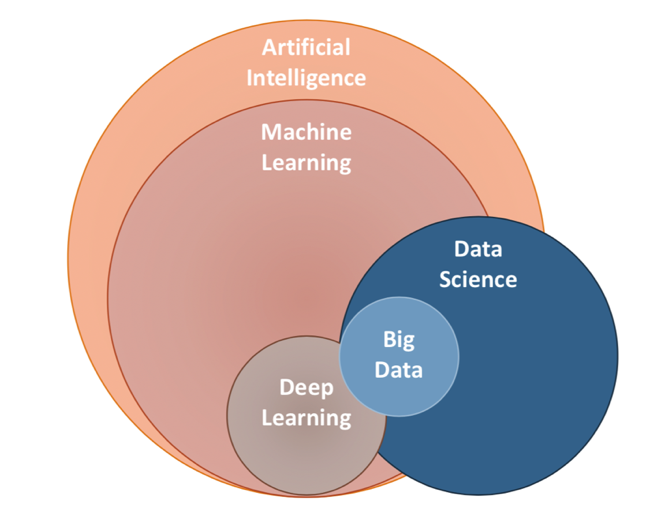
\includegraphics[scale=0.51]{img/Marco Teorico/Expertiz.png} 
	\caption{Diagrama de Venn con las subáreas de la IA}
\end{figure}


\doublespacing
\section{Machine Learning}
\spacing{1.5}
Los problemas por computadora se solucionan con un algoritmo que le indica a la máquina los pasos a seguir. En un ejemplo clásico podemos usar un algoritmo de búsqueda, donde el dato a buscar sería la entrada y su salida sería si se encontró o no y en cuánto tiempo. Es bien conocido que para resolver el problema de búsqueda existen variados algoritmos, algunos más eficientes que otros, aplicables a un contexto u otro de mejor forma, solucionando el mismo problema.\\
\par Asimismo, la publicidad en el celular es un ejemplo de cómo los algoritmos de ML están aplicándose en la vida cotidiana. Estos algoritmos utilizan técnicas de análisis de datos y aprendizaje automático para comprender los patrones de comportamiento y preferencias de los usuarios a partir de la información de navegación y otros datos recopilados en sus dispositivos móviles. Además de la publicidad en el celular, los algoritmos de ML también están siendo utilizados en una variedad de aplicaciones, como la recomendación de productos y servicios, la detección de fraudes, la mejora de la eficiencia en la toma de decisiones y la optimización de la experiencia del usuario.\\
\par En el año 1959, Arthur Samuel \cite{samuel1959machine}, definió el concepto de ML como:

\begin{quote}
	"\emph{Un campo de estudio que le entrega a los computadores la habilidad de aprender sin haber sido explícitamente programado para eso}"
\end{quote}


Tom M. Mitchell en 1977 \cite{mitchell1997machine}, define el ML, en uno de sus libros, como:
\begin{quote}
	\emph{“El estudio de algoritmos de computación que mejoran automáticamente su rendimiento gracias a la experiencia. Se dice que un programa informático aprende sobre un conjunto de tareas, gracias a la experiencia y usando una medida de rendimiento, si su desempeño en estas tareas mejora con la experiencia”}
\end{quote}

\par Es decir, estos algoritmos aprenden y mejoran solos gracias a las experiencias pasadas, a diferencia de modelos en los que un experto puede asignar reglas y modela gracias a sus conocimientos.\\
\par ML utiliza algoritmos para analizar grandes cantidades de datos y descubrir patrones y relaciones en ellos. Una vez que el algoritmo ha aprendido de estos datos, puede aplicar lo que ha aprendido a un nuevo conjunto de datos y utilizarlo para tomar decisiones o hacer predicciones. \cite{murdoch2019interpretable}.\\
\par En este sentido, el ML permite a las máquinas aprender de los datos y utilizar ese conocimiento para mejorar sus decisiones y predicciones. Esto es una gran ventaja en comparación con los enfoques tradicionales, en los que un programador humano debe escribir una serie de reglas y lógica para tomar decisiones. Con el aprendizaje automático, las máquinas pueden aprender por sí mismas y mejorar con el tiempo sin la necesidad de programación adicional.\\

\doublespacing
\subsection{Machine Learning: Tipos de Aprendizajes}
\spacing{1.5}
ML contempla dos enfoques o tipos de aprendizaje bastante usados, el aprendizaje supervisado y el aprendizaje no supervisado.\\


\doublespacing
\subsubsection{Aprendizaje Supervisado}
\spacing{1.5}
Este enfoque es un método de análisis de datos que necesita de algoritmos que aprendan a través de entrenamiento, en el cual el algoritmo es alimentado con datos etiquetados, atributos y la variable objetivo en cada iteración.\\
\par El aprendizaje supervizado se divide en dos tareas comunes: clasificación y regresión.\\
\par La tarea de clasificación se utiliza para predecir una categoría o clase para un nuevo conjunto de datos. Por ejemplo, un algoritmo de clasificación puede ser entrenado con datos sobre diferentes tipos de frutas y sus características para predecir si una nueva fruta es una manzana o una pera.\\
\par La tarea de regresión se utiliza para predecir un número o valor continuo. Por ejemplo, un algoritmo de regresión puede ser entrenado con datos sobre la relación entre la edad de una persona y su salario para predecir el salario de una persona en función de su edad.\\
\par En resumen, el aprendizaje supervisado es una técnica muy útil y ampliamente utilizada en el ML para hacer predicciones precisas sobre nuevos datos. A través de la tarea de clasificación y regresión, se pueden solucionar una amplia variedad de problemas y aplicaciones en una amplia gama de industrias \cite{murdoch2019interpretable}. \\


\doublespacing
\subsubsection{Aprendizaje No Supervisado}
\spacing{1.5}
El aprendizaje no supervisado tiene datos sin etiquetar que el algoritmo tiene que entender por si mismo, el propósito es descubrir patrones ocultos en ellos. Si nosotros le pedimos a nuestro programa \textit{"predecir \textbf{Y} para nuestros datos \textbf{A}"},  nosotros deberíamos \textit{“pedirle que nos provea de la información de nuestros datos \textbf{A}"} \cite{murdoch2019interpretable}.\\
\par Las tareas más comunes dentro del aprendizaje no supervisado son el \emph{clustering} y \emph{dimension reduction}, los cuales no son objeto de nuestro estudio por lo que solo son mencionados en esta parte del documento.\\


\doublespacing
\subsection{Técnicas de Clasificación}
\spacing{1.5}
Para que nuestro modelo de ML funcione, debemos categorizar los datos de entrada y salida, reconociendo atributos del elemento a clasificar y utilizando el conocimiento adquirido durante el entrenamiento del algoritmo para asignar un valor a la variable objetivo de dicho elemento.\\
\par La clasificación de datos es un proceso que consta de dos etapas, la etapa de aprendizaje donde es construido el modelo, y la etapa de clasificación donde el modelo es usado para predecir las etiquetas de clases de los datos dados \cite{han2012data}.\\
\par En la \textit{primera} etapa de aprendizaje o entrenamiento del algoritmo, se construye el modelo utilizando una serie de datos que sirven de base para el conocimiento del algoritmo, para lograr esto, es que se le entrena utilizando un set de entrenamiento, que no son más que tuplas de datos etiquetados tanto en sus atributos como en su variable objetivo. Una tupla X, generalmente es representada por un vector n-dimensional llamado vector de atributos $ X = (x_{1}, x_{2}, ..., x_{n}) $.\\
\par En la \textit{segunda} etapa, el algoritmo ya ha sido entrenado con los datos de entrenamiento y está listo para la clasificación de una variable $ x $. El algoritmo implementado
será capaz de tomar los atributos de dicha variable, analizarlos y tomar una decisión en los resultados, basándose en los datos que fueron entregados anteriormente.\\
\par En la clasificación veremos algunas de las técnicas clásicas de ML, pertenecientes al enfoque de los algoritmos de aprendizaje supervisado, definiendo brevemente cada una de ellas.\\


\doublespacing
\subsection{Decision Tree (Árbol de Decisión)}
\label{sec:DT}
\spacing{1.5}
Este algoritmo que se utiliza como herramienta de apoyo gráfico o modelo de decisiones con sus posibles consecuencias, también a veces son representados los costos y su posible utilidad (CART, Classification and Regression Trees). Este método se crea particionando la entrada recursivamente en distintas ramas, siendo que la idea es crear un camino desde la raíz hasta las hojas, donde cada nodo podría ser una condición así, si se cumple la condición se sigue por el camino de decisión, o por la otra rama si no se llegara a cumplir la condición \cite{Harrington2012}.\\
\par La creación del modelo se puede representar en la ecuación \ref{eq:Ecuación del Modelo Decision Tree}:\\

\begin{Large}
	\begin{equation}
		f(x)=E[y|x]=\sum_{m=1}^{M}w_{m}I(x \in R_{m})=\sum_{m=1}^{M}w_{m}\phi(x;v_{m})
		\label{eq:Ecuación del Modelo Decision Tree}
	\end{equation}
\end{Large}

Donde:

\begin{itemize}
	\item $R_{m}$ representa la región de $m$.
	\item $w_{m}$ es respuesta media a esa región.
	\item $v_{m}$ codifica la elección de la variable por la que dividir y el valor límite de la división.
\end{itemize}


\begin{figure}[H]
	\centering
	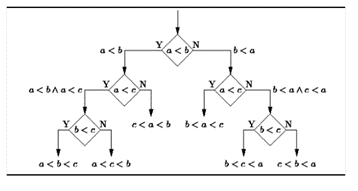
\includegraphics[scale=1.3]{img/Marco Teorico/arbol de desicion.png} 
	\caption{Ejemplo de un problema aplicando Árbol de Decisiones}
	\label{fig:padt2}
\end{figure}

\par En la Figura \ref{fig:padt2} se presenta un ejemplo del modelo que se puede generar. Las condiciones se dan como alternativas de caminos a seguir.\\

\doublespacing
\subsubsection{Usos para los Decision Tree}
\spacing{1.5}
Al ser de fácil implementación, los Decision Tree son usados en diversas áreas, siendo las instituciones financieras las más comunes, ayudando a clasificar clientes, estableciendo sus riesgos o posibilidades financieras \cite{Harrington2012}.\\
\par En el área de la salud son empleados para diagnósticos de infecciones a la sangre o predicción de ataque al corazón en pacientes de alto riesgo \cite{Harrington2012}.\\
\par En el seguimiento de movimiento, los árboles de decisión se utilizan para analizar los movimientos de un objeto en un video y predecir su ubicación en el siguiente cuadro. Esto se logra mediante la creación de un modelo de decisión que tome en cuenta factores como la velocidad, la dirección y el tamaño del objeto. \cite{Harrington2012}.\\
\par En el reconocimiento facial, los árboles de decisión se utilizan para identificar a una persona en un video o imagen. Esto se logra mediante la creación de un modelo de decisión que tome en cuenta características como la forma de la cara, el tamaño de la nariz y la distancia entre los ojos \cite{Harrington2012}.\\

\doublespacing
\subsubsection{Ventajas y Desventajas}
\spacing{1.5}
Las ventajas de esta técnica de ML es su bajo costo computacional y simple interpretación de resultados. \\
\par La mayor desventaja es que la técnica es propensa a caer en el sobreajuste, siendo a veces manipulada por quien lo implemente \cite{Harrington2012}.\\

\doublespacing
\subsection{Random Forest (Bosque Aleatorio)}
\label{sec:RF}
\spacing{1.5}
El algoritmo de Random Forest es una técnica de aprendizaje supervisado que genera múltiples árboles de decisión sobre un conjunto de datos de entrenamiento: los resultados obtenidos se combinan para obtener un modelo único más robusto en comparación con los resultados de cada árbol por separado \cite{breiman2001random}.\\
\par Cada árbol se obtiene mediante un proceso de dos etapas:

\begin{itemize}
	\item[1-.] Se genera un número considerable de árboles de decisión con el conjunto de datos. Cada árbol contiene un subconjunto aleatorio de variables $m$ (predictores) de forma que $m < M$ (donde M = total de predictores).
	\item[2-.] Cada árbol crece hasta su máxima extensión.
\end{itemize}

\par En la Figura \ref{fig:Random Forest} se muestran las etapas mencionadas anteriormente:

\begin{center}
	\begin{figure}[H]
		\centering
		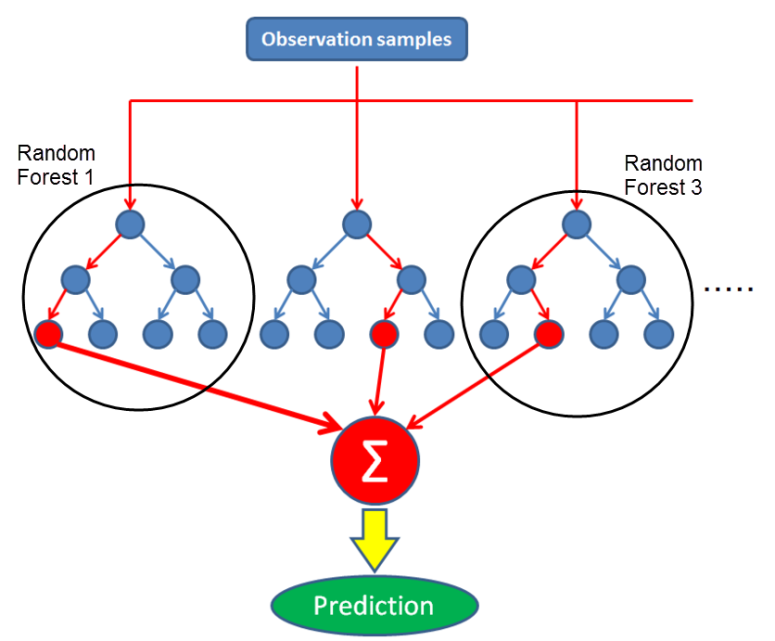
\includegraphics[scale=0.5]{img/Marco Teorico/random-forest-1.png} 
		\caption{Ejemplo de la secuencia en un Random Forest}
		\label{fig:Random Forest}
	\end{figure}
\end{center}


\doublespacing
\subsubsection{Ventajas y Desventajas}
\spacing{1.5}

Las principales ventajas de Random Forest son su simpleza al entrenar el modelo, desempeño muy eficiente, certera en base de datos grandes, mantiene su precisión con proporciones grandes de datos perdidos \cite{canovas2017modification}.\\
\par Algunas desventajas son la visualización gráfica donde los resultados pueden ser difíciles de interpretar, tiene poco control sobre lo que hace el modelo (en cierto sentido es como una caja negra) \cite{canovas2017modification}.\\

\doublespacing
\subsection{Naïve Bayes (Redes de Bayes)}
\label{sec:NB}
\spacing{1.5}
Naïve Bayes es un algoritmo de clasificación probabilístico que utiliza la teoría de probabilidad y estadística para realizar clasificaciones. Es llamado \emph{Naive} porque supone que todas las características son independientes entre sí, lo que en la mayoría de los casos no es verdad. Este teorema calcula la probabilidad de una clase dado un conjunto de características. La probabilidad se calcula multiplicando la probabilidad a priori de cada clase con la probabilidad condicional de cada característica dada esa clase\cite{Vembandasamy2015}. \\
\par Este algoritmo es muy eficiente y rápido que se utiliza en una amplia gama de aplicaciones, incluyendo la detección de spam, la categorización de documentos y la clasificación de texto. Además, es uno de los algoritmos más simples y fáciles de implementar en Machine Learning \cite{Vembandasamy2015}.\\

\par La fórmula condicional se expresa en la ecuación \ref{eq:Probabilidad condicional}:\\
\begin{Large}
	\begin{equation}
		P(A|B)=\frac{P(A \cap B)}{P(B)}= \frac{(\frac{\#casos favorables A \cap B}{\#casos posibles})}{(\frac{\#casos favorables B}{\#casos posibles})}
		\label{eq:Probabilidad condicional}
	\end{equation}
\end{Large}\\
\par Desarrollando la ecuación nos queda en la ecuación \ref{eq:Probabilidad condicional resumida}\\
\begin{Large}
	\begin{equation}
		P(A_{i}|B)=\frac{P(B|A_{i})*P(A_{i})}{P(B)}
		\label{eq:Probabilidad condicional resumida}
	\end{equation}
\end{Large}\\
\par Donde cada evento es tomado como se demuestra en la ecuación \ref{eq:Probabilidadn del evento}\\
\begin{large}
	\begin{equation}
		P(A|B)= P(B_{1}|A) \times P(B_{2}|A) \times … \times P(B_{n}|A) \times P(A)
		\label{eq:Probabilidadn del evento}
	\end{equation}
\end{large}\\

Donde:
\begin{itemize}
	\item $P(A_{i})$ son las probabilidades a priori.
	\item $P(B|A_{i})$ es la probabilidad de $B$ dado $A_{i}$.
	\item $P(A_{i}|B)$ son las probabilidades a posteriori.
	\item $P(B)$ es la probabilidad total de $B$.
\end{itemize}


\par Las Redes de Bayes se generan de reglas de decisión donde participan activamente las probabilidades que ocurren referente a eventos, siendo que en base a esas probabilidades y resultados obtenidos, se toman decisiones sobre cuál arco de red moverse. Al final del proceso, el resultado será dado por el valor del nodo final de la red \cite{Bell15}.\\


\doublespacing
\subsubsection{Ventajas y Desventajas}
\spacing{1.5}
Las ventajas de esta técnica de ML son su fácilidad para implementarla, eficiencia y rápidez de tiempo de entrenamiento, buen rendimiento en textos y documentos, además no requiere mucha información para ser entrenado.\\
\par Las desventajas son la suposición de independencia de las variables (siendo que en muchos casos las características no son independientes), vulnerable al ruido, no es óptimo para características no correlacionadas \cite{Bell15}.

\doublespacing
\subsection{Logistic Regression (Regresión Logística)}
\label{sec:LR}
\spacing{1.5}
El algoritmo Logistic Regression modela la relación entre distintas variables utilizando una medida de error que se intentará minimizar en un proceso iterativo para poder realizar predicciones acertadas, llevando a cabo una clasificación binaria con una distribución Bernoulli en vez de Gaussian y después realiza una combinación lineal de las variables en un rango de 0 a 1 \cite{ Stoltzfus2011}.\\
\par La ecuación lineal \ref{eq:Ecuación Lineal} se debe ajustar:\\
\begin{Large}
	\begin{equation}
		y(X)=W^{T}X + \epsilon = \sum_{j=1}^{D}w_{j}x_{j} + \epsilon
		\label{eq:Ecuación Lineal}
	\end{equation}
\end{Large}\\ 
\par $W^{T}X$ representa el producto escalar de entrada X.
\par $W$ e $Y$ son vectores de pesos $\in$ $\lbrace 0,1 \rbrace$.\\

\par Ahora mostrando la ecuación \ref{eq:Distribución de Bernoulli} la distribución de Bernoulli:\\
\begin{Large}
	\begin{equation}
		p(y|x,w) = Ber(y|u(x))
		\label{eq:Distribución de Bernoulli}
	\end{equation}
\end{Large}
\begin{center}
	El resultado del intervalo quedaría $0 \leq u(x) \leq 1$.\\
\end{center}
\par El resultado de la ecuación nos ayudará a predecir valores con la mejor respuesta a partir del menor error posible, teniendo un valor continuo entre 0 y 1. Si existe un valor mayor o igual a 0.5, la clase será 1, en cambio si es menor será 0. Todo esto ocurre porque el algoritmo de Logistic Regression predice un valor en vez de una clase en función de las variables utilizadas.\\

\doublespacing
\subsubsection{Ventajas y Desventajas}
\spacing{1.5}
Logistic Regression al igual que las técnicas anteriores es fácil de implementar, interpretar y muy eficiente al momento de entrenar, incluyendo que no hace suposiciones sobre distribuciones de clases en el espacio de características y es muy rápido para clasificar registros desconocidos.\\
\par Las principales desventajas de esta técnica radican en si el número de observaciones es menor que el número de características, no se debe utilizar la regresión logística; de lo contrario, puede provocar un sobreajuste y la difícil obtención de relaciones complejas.  Para trabajos más potentes y compactos existen la Artificial Neural Networks, las cuales pueden superar fácilmente este algoritmo. \cite{Harrington2012}. \\


\doublespacing
\subsection{Support Vector Machine (Máquina de Vectores de Soportes)}
\spacing{1.5}
Esta técnica no será parte de los algoritmos que se analizarán en este trabajo, sin embargo, se explicará en qué consiste su proceso, debido a que es una de las técnicas clásicas de ML.\\
\par El algoritmo Support Vector Machine (SVM, por sus siglas en inglés) pertenece al ML supervisado que se utiliza para clasificación y regresión. Es un algoritmo de ML basado en el aprendizaje de modelos. El objetivo de SVM es encontrar un hiperplano que separe los datos en dos clases, de manera que los datos de una clase se encuentren en un lado del hiperplano y los datos de la otra clase se encuentren en el otro lado. El hiperplano es elegido de tal manera que maximice la margin, es decir, la distancia entre el hiperplano y los datos más cercanos. Estos datos más cercanos son conocidos como vectores de soporte. En este método, una función elige la predicción del valor esperado del caso mediante una entrada de datos \cite{Dantas2021}.\\


\doublespacing
\subsection{Artificial Neural Networks (Redes Neuronales Artificiales)}
\spacing{1.5}
Esta técnica no será parte de los algoritmos que se analizarán en este trabajo, sin embargo, se explicará en qué consiste su proceso, debido a que es una de las técnicas clásicas de ML.\\
\par La Artificial Neural Networks (ANN, por sus siglas en inglés) son un tipo de modelo de aprendizaje automático que simula la estructura y función de las redes neuronales en el cerebro humano. Una ANN está compuesta por nodos o "neuronas" que están conectados entre sí y transmiten información a través de las conexiones. Posee una arquitectura de procesadores múltiples interconectados para simular la estructura humana \cite{salas2004redes}. Las ANN se utilizan para realizar tareas como la clasificación, la regresión, la traducción de idiomas, la generación de texto y la identificación de patrones en grandes conjuntos de datos.\\
\par Los métodos de aprendizaje que se emplean por lo regular son arquitecturas de redes neuronales tradicionales, donde solo se tienen dos o tres capas ocultas, imitando la operación que realiza el cerebro (Azath et al., 2020), en cambio, el DL aprenden sobre la marcha y su arquitectura puede llegar a tener 150 capas ocultas. \\

\doublespacing
\subsection{Deep Belief Network (Red de creencias profundas)}
\spacing{1.5}
Esta técnica no será parte de los algoritmos que se analizarán en este trabajo, sin embargo, se explicará en qué consiste su proceso, debido a que es una de las técnicas clásicas de ML.\\
\par La Deep Belief Network (DBN, por sus siglas en inglés) son un tipo de ANN que se utiliza para modelar relaciones complejas entre variables. Una DBN es una combinación de varias redes neuronales artificiales y se entrena de forma no supervisada para aprender patrones y relaciones en los datos.  La DBN tiene múltiples niveles de capas y variables ocultas, ellas están conectadas entre las capas visibles y ocultas, pero no en las capas visibles – visible u oculta – oculta \cite{PuertaBarrera2015}.\\
\par Las DBN se utilizan en aplicaciones como la clasificación de imágenes, la detección de fraudes, la recomendación de productos y la identificación de tendencias en los datos. \\

\doublespacing
\subsection{Feedforward Artificial Neural Network (Red Neuronal de Retroalimentación)}
\spacing{1.5}
Esta técnica no será parte de los algoritmos que se analizarán en este trabajo, sin embargo, se explicará en qué consiste su proceso, debido a que es una de las técnicas clásicas de ML.\\
\par Las Feedforward Artificial Neural Network (FANN) es la sucesora de ANN, trabajándose en diversos campos y aplicándose más en DL. Este algoritmo se caracteriza por tener una estructura en la que los datos fluyen en una dirección, desde las entradas hasta las salidas, sin retroalimentación o retroalimentación en ciclo. En la FANN, los datos se introducen en la red en la capa de entrada y se procesan a través de varias capas intermedias, cada una compuesta por una serie de nodos o neurones. Los nodos realizan cálculos simples en base a las entradas recibidas y generan una salida, que a su vez es procesada por la capa siguiente. La salida final de la red se produce en la capa de salida \cite{salas2004redes}.\\ 
\par La FANN se utiliza en una amplia variedad de aplicaciones, incluyendo la clasificación de imágenes, la detección de fraudes, la recomendación de productos y la identificación de tendencias en los datos.\\

\doublespacing
\subsection{Recurrent Neural Networks (Redes Neuronales Recurrentes)}
\spacing{1.5}
Esta técnica no será parte de los algoritmos que se analizarán en este trabajo, sin embargo, se explicará en qué consiste su proceso, debido a que es una de las técnicas clásicas de ML.\\
\par La Recurrent Neural Networks (RNN, por sus siglas en inglés) son un tipo de red neuronal artificial que se utiliza en el ML. A diferencia de la FANN, las RNN tienen una estructura que permite la retroalimentación, lo que les permite tomar en cuenta la secuencia temporal de los datos. Las RNN asigna parámetros únicos para representar a cada dato en una secuencia \cite{arana2021redes}.\\
\par Para poder tener el control y no sufrir interrupciones sobre la secuencia. Su arquitectura es multicapa que comparte pasos entre los datos espaciados secuencialmente para poder unir la información. Su arquitectura se va incrementando con la conexión de nodos adyacentes a través de la adición de ciclos dentro de la red.\\
\par Las RNN son reconocidas por obtener información de datos secuenciales como lo son el procesamiento del lenguaje natural, videos y subtitulación de imágenes.\\


\doublespacing
\section{Deep Learning (Aprendizaje Profundo)}
\spacing{1.5}
Las técnicas de ML están limitadas en el procesamiento de los datos naturales en forma cruda y para dar solución a la problemática se creó el aprendizaje profundo. La comprensión de la IA y cómo puede llegar a igualar los comportamientos humanos, inclusive en el aprendizaje, a veces superándonos, fue un gran acontecimiento que se debe a la gran contribución de Alan Turing \cite{Carola}. El DL como subárea del ML entra en acción cuando los datos tienen demasiadas características, son enormes, se requiere de un nivel de precisión altísima y el ML no puede ofrecer completamente los resultados deseados.\\


\doublespacing
\subsection{Convolutional Neural Networks (Redes Neuronales Convolucionales)}
\spacing{1.5}
El DL ha demostrado muy buenos resultados para la resolución de problemas, en cambio, las limitaciones, sobre todo en el campo de la imagenología, ha hecho que se elabore un método diferente para que exista un análisis más preciso al momento de analizar una imagen. Este método se llama Convolutional Neural Networks (CNN), que tiene una arquitectura con mejor rendimiento para las tareas de relaciones complejas \cite{Pena-Torres}. \\
\par Desde el año 2012, las arquitecturas basadas en CNN para visión artificial han crecido muchísimo; sin embargo, no todas han sido eficientes para ocuparse en tareas de visión artificial (Figueroa Flores, 2021), siendo el Grupo de Geometría Visual (VGG) de la Universidad de Oxford \cite{Simonyan2015} una de las arquitecturas más utilizadas para las tareas de procesamiento de visión artificial. \\
\par Las CNN se forman usando tres tipos de capas, los cuales son capas convolucionales, capas de pooling y capas totalmente conectadas, como se muestra en la Figura \ref{fig:CNN}.\\

\begin{figure}[H]
	\centering
	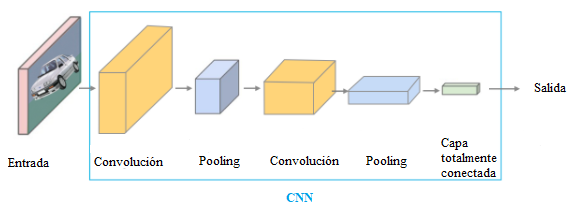
\includegraphics[scale=0.7]{img/Marco Teorico/convulcioinales.png}  
	\caption{Descripción del funcionamiento de una CNN \cite{Carola}}
	\label{fig:CNN}
\end{figure}

\par Para la CNN existen dos arquitecturas básicas, las cuales son CNN que entrega una salida para toda la imagen, como en la Figura \ref{fig:CNN} y la Fully Convolutional networks que posee un codificador y decodificador, entrega una compresión de la información y su salida es por pixel. En las arquitecturas CNN exiten varios ejemplos, como lo son AlexNet, entrenado con ImageNet, GoogLeNet que posee 22 capas y sus neuronas son más complejas, entre otras \cite{NIPS2012_c399862d}.\\


\doublespacing
\subsection{Neural Networks for Scarce Data Domains  (Redes neuronales para dominios de datos escasos)}
\spacing{1.5}
Las redes neuronales pueden ser muy efectivas para abordar problemas en los que los datos son escasos \cite{Carola}. Sin embargo, cuando los datos son escasos, es esencial utilizar un enfoque diferente para entrenar las redes neuronales. Fei-Fei et al. \cite{Fei-Fei2006} demostraron que es posible aprender nuevas categorías, una o pocas muestras por clase, aprovechando las categorías aprendidas anteriormente. \\

\doublespacing
\section{Otros conceptos importantes para la investigación relacionados con la IA}
\spacing{1.5}
Existen muchos conceptos importantes que tienen relación con la IA, en esta sección definimos conceptos relevantes para lo que sigue de este trabajo.

\doublespacing
\subsection{Dataset}
\spacing{1.5}
Un Dataset se refiere a una colección de datos que generalmente tiene la misma forma que una tabla de base de datos o una hoja de cálculo \cite{Astudillo2021}. Un conjunto de datos consiste en un conjunto de ejemplos o casos. Una instancia también se denomina fila en una tabla de base de datos o, a veces, caso en estadística. Las funciones (columnas de la tabla) también tienen muchos nombres diferentes. Los estadísticos llaman atributos a las variables independientes o predictoras que se proporcionan como entradas. En investigación de operaciones, se habla de variables explicativas. La variable objetivo, cuyo valor se va a predecir, generalmente se denomina variable dependiente en estadística. La terminología puede ser un poco confusa; las variables independientes pueden no ser independientes entre sí (o de nada), y las variables dependientes no necesariamente dependen de todas las variables independientes. Es importante ser claro: la variable objetivo no se utiliza para predecirse a sí misma. Sin embargo, los valores anteriores de la variable objetivo pueden ser útiles para predecir valores futuros, por lo que estos valores pasados pueden incluirse como función \cite{provost2013data}.\\
\par En el Dataset la reducción de datos es importante y éste intenta tomar un gran conjunto de datos y reemplazarlo con un conjunto de datos más pequeño que contiene la mayor parte de la información importante en el conjunto más grande. Los conjuntos de datos más pequeños pueden ser más fáciles de manejar. Cuanto más pequeño sea el conjunto de datos, mejor información se podrá descubrir. Por ejemplo, grandes conjuntos de datos sobre preferencias de visualización de películas, se pueden reducir a un conjunto de datos más pequeño, que revela las preferencias de gustos del consumidor ocultas en los datos de visualización (como las preferencias de género de la audiencia). La reducción de datos a menudo se asocia con la pérdida de información \cite{provost2013data}.\\

\doublespacing
\subsection{Matriz de Confusión}
\label{sec:mc}
\spacing{1.5}
En el campo de la IA, en especial en el problema de la clasificación estadística, una matriz de confusión es una herramienta que permite la visualización del desempeño de un algoritmo que se emplea en aprendizaje supervisado .
\par La estructura de la matriz de confusión 2x2 o más (dependiendo del número de clases), donde cada fila representa una clase real y cada columna representa una clase predicha por el modelo \cite{Harrington2012}:

\begin{itemize}
	\item \textbf{Positivo (P)}: La observación es positiva (por ejemplo, el paciente \textit{tiene} COVID).
	\item \textbf{Negativo (N)}: La observación no es positiva (por ejemplo, el paciente \textit{no tiene} Covid).
	\item \textbf{Verdadero Positivo (TP)}: Resultado en el que el modelo \textit{predice correctamente la clase positiva}.
	\item \textbf{Verdadero Negativo (TN)}: Resultado donde el modelo \textit{predice correctamente la clase negativa}.
	\item \textbf{Falso Positivo (FP)}: También llamado error de tipo 1, resultado donde el modelo \textit{predice incorrectamente la clase positiva cuando en realidad es negativa}.
	\item \textbf{Falso Negativo (FN):} También llamado error de tipo 2, un resultado en el que el modelo \textit{predice incorrectamente la clase negativa cuando en realidad es positiva}.
\end{itemize}

\par La matriz de confusión se utiliza para calcular métricas de rendimiento como la precisión, la exhustividad y la medida F1.

\doublespacing
\section{Aspectos de la salud y la enfermedad}
\spacing{1.5}
La salud es uno de los aspectos más importantes en la vida, muchas veces nuestra salud se ve afectada por factores externos o internos a nuestra persona. “Este concepto involucra un estado completo de bienestar físico, mental y social, y no solamente la ausencia de afecciones o enfermedades” (Wold Health Organization, 1946).  \\

\doublespacing
\subsection{Accidente Cerebro Vascular}
\spacing{1.5}
\par Un Accidente Cerebro Vascular es la detención del flujo de sangre a una parte del cerebro. En ocasiones se le llama “Ataque Cerebral”. Si el flujo sanguíneo se detiene por más de pocos segundos, el cerebro no recibirá nutrientes ni oxígeno, causando una muerte y un daño permanente en la zona afectada \cite{Garcia2019}.
\par Existen dos tipos de ACV, Isquémicos y Hemorrágicos.\\

\doublespacing
\subsection{Accidente Cerebro Vascular Isquémico}
\spacing{1.5}
\par Los ACV Isquémicos son los más comunes, generalmente, son causados por un coágulo sanguíneo (masas que se presentan cuando la sangre se endurece, pasando de líquida a sólida) que bloquea el vaso sanguíneo del cerebro, lo que provoca la muerte de células cerebrales. Esto puede causar daño cerebral y resultar en una variedad de síntomas y discapacidades, incluyendo debilidad en un lado del cuerpo, problemas de habla, visión doble, pérdida de la capacidad de caminar y, en casos graves, la muerte \cite{Adams1993}.\\
\par Existen dos tipos de ACV Isquémicos: transitorios y permanentes \cite{Garcia2019}. Los transitorios se producen cuando la sangre no llega al cerebro por unos instantes, en cambio, el permanente es producido cuando la sangre no llega al cerebro por un tiempo prolongado, también es llamado Infarto Cerebral. \\

\doublespacing
\subsection{Síntomas ACV Isquémico}
\spacing{1.5}
\par Los síntomas de un ACV Isquémico pueden ser:
	\begin{itemize}
		\item Entumecimiento o debilidad repentina de la cara, brazo o pierna (especialmente en un lado del cuerpo).
		\item Confusión repentina, dificultad para hablar o entender el lenguaje.
		\item Dificultad repentina para ver con uno o ambos ojos.
		\item Problemas para caminar repentino, mareos, pérdida de equilibrio o coordinación.\\
	\end{itemize}
	
\doublespacing
\subsection{Categorías de los ACV}
\spacing{1.5}
\par En los ACV para ayudar a optimizar el tratamiento específico, existen categorías que son identificadas por la escala de TOAST \cite{Adams1993}.\\
\par La primera categoría es la enfermedad Aterotrombótica aterosclerótica de gran vaso, se basa en la reducción de tejido sanguíneo medio o grande en el cerebro, con ubicación cortical o subcortical, con localización vertebrobasilar o carotídea, donde se encuentra presente una aterosclerosis u obstrucción con estenosis u oclusión de las arterias craneales. También la aterosclerosis sin estenosis con menos factores de riesgo se puede encontrar presente en esta categoría. La segunda categoría es el Cardioembolismo, es una reducción de tejido sanguíneo medio o grande, de localización cortical, en la que existe una cardiopatía embolígena \cite{Molina2018}. La tercera categoría es la enfermedad oclusiva de pequeño vaso infarto lacunar, es una reducción de tejido sanguíneo de tamaño pequeño, en el sector de una arteria perforante cerebral que puede provocar una oclusión en el transporte de nutrientes. La cuarta categoría se debe a otras causas, de tamaño o localización variable que no están en las tres categorías anteriores, y que pueden producir enfermedades metabólicas, alteraciones de la coagulación, displacia fibromuscular, etc. La quinta categoría hace énfasis a los orígenes desconocidos con estudios incompletos o completos, por más de una etiología \cite{Radu2017}.\\


\doublespacing
\subsection{Tratamiento en los ACV}
\spacing{1.5}
Las ayudas diagnósticas proveen información sobre el grado de lesión y la identificación de la lesión  como las imágenes, escogiendo el tratamiento más adecuado para la lesión \cite{Wintermark2013}. En el tratamiento como recomendación general, el soporte de la vía aérea y la asistencia ventilatoria es fundamental, ya que los pacientes pueden presentar alteración en el estado de conciencia o disfunción bulbar que afecte la vía aérea. Además, se recomienda lograr saturaciones de oxígeno mayores a 94\% aún si implica oxígeno suplementario. Agregando a lo anterior se debe monitorizar la hiperglicemia, porque si llega a perdurar por más de 24 horas, el pronóstico se asocia a un peor desenlace \cite{Garcia2019}.\\
\par El tratamiento específico para un ACV Isquémico depende del tamaño y la ubicación del coágulo, así como de la gravedad de los síntomas. Algunos pacientes pueden requerir terapia médica, como anticoagulantes o medicamentos que disuelvan el coágulo, mientras que otros pueden necesitar cirugía o procedimientos endovasculares para extraer o disolver el coágulo. Además del tratamiento médico, los pacientes que han sufrido un ACV isquémico pueden necesitar rehabilitación para recuperar la función cerebral y física perdida. Esto puede incluir terapia física, terapia ocupacional, terapia de habla y otros tipos de rehabilitación \cite{Garcia2019}.\\


\doublespacing
\subsection{Escala de ACV del National Institute of Health (NIHSS)} 
\label{sec:NIHSS}
\spacing{1.5}
La escala de NIHSS mide el daño neurológico ocasionado en el paciente con ACV. Esta escala se ha convertido en una de las herramientas más útiles para monitorear neurológicamente en Unidades de ACV, tanto en la evaluación inicial del paciente, como para su seguimiento. El seguimiento puede arrojar mejoría o empeoramiento neurológico \cite{cien2001}. \\
\par La escala contiene 11 items (desarrollada serían 15), que permiten valorar de forma rápida: funciones corticales, pares craneales superiores, función motora, sensibilidad, coordinación y lenguaje \cite{cien2001}. La escala tiene un minimo de 0 puntos y un máximo de 42 puntos.\\
\par La clasificación de la puntación se presenta de la siguiente manera (Montaner et al, 2006) \cite{montaner2006escala}:

\begin{itemize}
	\item 0 punto: sin déficit.
	\item 1 punto: déficit mínimo.
	\item 2-5 puntos: leve.
	\item 6-15 puntos: moderado.
	\item 15-20 puntos: déficit importante.
	\item > 20 puntos: grave.\\
\end{itemize}

\par La puntuación inicial tiene buen valor pronóstico \cite{heinemann1997measurement}, considerando que un NIHSS 	$\leq$ 6 corresponde con una excelente recuperación neurológica y cada incremento en un punto empeoraría la evolución \cite{Adams1993}. Pacientes con fibrilación auricular, una NIHSS $\geq$ 16 ya se considera de muy mal pronóstico \cite{frankel2000predicting}.\\

	% Trabajos Relacionados
	\doublespacing
\chapter{TRABAJOS RELACIONADOS}
\label{sec:trabajos relacionados}
\spacing{1.5}
\lettrine[lines=4, slope=0.2em, findent=0.2em, nindent=0.6em]{E}{l}  análisis del estado del Arte contempla una revisión bibliográfica, contextualizando los avances en la investigación acerca de la IA y el área de salud. A continuación daremos a conocer algunos trabajos de los últimos años.\\

\par Los avances en hospitales de países desarrollados han permitido la implementación de la IA en sus sistemas, lo que implica nuevos desafíos, como lo son el procesamiento de grandes volúmenes de información,  datos incompletos debido a la incompatibilidad de los sistemas en que se registran o incluso la presión de entregar una investigación o producto sin prolijidad y beneficio real para las personas \cite{Nagendran2020}. Google es un ejemplo claro de esta situación donde  sus algoritmos con IA presentan los problemas mencionados anteriormente.\\

\par Con el aumento de las tecnologías en el campo médico y avance de las técnicas de ML, se ha desarrollado un interés por el mundo científico para predecir algún proceso o secuela después de un ACV. Investigadores en el 2019 \cite{Heo2019}, realizaron estudio utilizando Random Forest, Redes Neuronales y Logistic Regression para predecir la prognosis de un paciente de ACV Isquémico tres meses después del evento inicial. Los autores deseaban predecir la mortalidad a los 3 años luego de salir de la rehabilitación con un algoritmo basado en Decision Tree. El mejor modelo fue Random Forest con la implementación del minority oversampling technique, el cual logró un nivel de predicción del modelo de 0.928  \cite{Scrutinio2020}. Yu et al. \cite{Yu2020} usaron técnicas de ML considerando el Decision Tree, siendo el objetivo clasificar la severidad del ACV Isquémico. El árbol se construyó originalmente con 13 variables, de 18 propuestas, los datos usados fueron de personas mayores de 65 años del National Institutes of Health Stroke Scale. Con esta técnica se logró tener un accuracy del 91.11\%, prediciendo el nivel de discapacidad, dentro de las 24 horas  y posteriormente a los 90 días  \cite{Xie2018}. Los predictores incluían información de exámenes de escáner, demografía e información clínica de los pacientes.\\

\par Con la herramienta de las imágenes nace la posibilidad de generar algoritmos para un método más actualizado en la detección de esta enfermedad y su futura prevención, puesto que existen variadas técnicas \cite{Wintermark2013} como la RM con DWI para la evaluación de presencia y extensión de isquemia posterior y la CTA y DSA para la trombosis de arteria. Continuando  con las investigaciones en imágenes, un estudio en Estados Unidos \cite{Garcia2019}  analizó 610.000 casos y 185.000 con recurrencia en el año 2019,  los cuales mostraban lesiones visibles en sus exámenes de imagenología, con dicha información se pudo sustentar que el manejo médico y la prevención secundaria son vitales para mermar las secuelas de los pacientes. Además de la necesidad de educar a la comunidad para reconocer algunos síntomas del ACV y así acudir al centro médico más cercano. Con base en el estudio anteriormente señalado podemos predecir que esta enfermedad llegará a un 6,2\% de la población en  países desarrollados, por esta razón es importante crear un modelo que nos permita predecir las secuelas o futuros problemas en el tratamiento, llevando a cabo una prevención exitosa, evitando la recurrencia. Por lo anteriormente expuesto es conveniente que el algoritmo para la atención deba estar basado en experiencias nacionles e internacionales \cite{Garcia2019}\\

\par La IA puede generar investigaciones DL relacionados a los estudios de Aprendizaje Profundo como estudio de revisión sistemática del diseño, estándares de informes y afirmaciones de los estudios de aprendizaje profundo \cite{Pang2017}. El objetivo de un modelo con DL es que logre ser  efectivo y eficaz y para ello es necesario trabajar con médicos expertos, a fin de que puedan  evaluar los diagnósticos mediante imágenes y contrastar los resultados obtenidos con la IA. Esta investigación posee una gran cantidad de datos como Ensayos controlados, datos Medline y ensayos que la Organización Mundial de la Salud posee desde 2010 hasta 2019, de los cuales se encontraron registros aleatorios de aprendizaje profundo con bajo nivel de sesgo. Por consiguiente la información que es emitida por los modelos de aprendizaje profundo para un diagnóstico más certero puede ser manipulada por los expertos, ya que los algoritmos \cite{Nagendran2020} son experimentales y pioneros en la materia.\\

\par Las redes de datos convolucionales demostraron, en Corea, ser una herramienta que predice con precisión los cuidados intensivos en servicios médicos (Kang et al., 2020), asumiendo que el modelo predictivo, basado en DL, es superior a las otras herramientas de predicción y puntuaciones convencionales \cite{Bioetica2022}. Cabe destacar, que el algoritmo de aprendizaje es muy eficiente por la cantidad de capas que puede poseer el modelo, puesto que entre más capas mayor puede ser el aprendizaje. Pese a las evidencias que demuestran la efectividad y el desempeño de las redes convolucionales, en términos de predicción, puede compararse o ser mejor al del humano, existe un miedo por la implementación en los sistemas de salud, lo que puede provocar que el crecimiento del DL, perezca de una base amplia para su desarrollo \cite{Nagendran2020}.\\

\par En el área de la implementación de un modelo con CNN, encontramos el trabajo de Chunjiao Dong , Chunfu Shao, Juan Li, and Zhihua Xiong del 2018, que desarrolla específicamente la predicción sobre los accidentes de tránsito \cite{shao2018improved}. Ellos demuestran una técnica novedosa con un modelo de regresión multivariable, que presenta la relación entre lo examinado y los accidentes de tránsito. Como resultados el modelo identifica las variables de entrada y representaciones de características de salida, aunque se haya reducido su magnitud, se conserva la información original. Además, el modelo propuesto explica mejor los problemas de heterogeneidad en predicción de accidentes de tráfico y puede ser aplicado a casos similares.\\

\par En este caso el modelo propuesto en contraste con el SVM en la categoría choque con daños menores es significativo (29.961\% versus 61.350\%), así es como la predicción medida por el RMSD se puede mejorar un  84,58\% y un 158,27\% en comparación con el modelo de aprendizaje profundo sin la capa de regresión y el modelo SVM.\\





\par El trabajo “Intelligence versus clinicians: systematic review of design, reporting standards, and claims of deep learning studies” del año 2020 \cite{Nagendran2020}, que utilizó el Deep Learning con Redes Neuronales Convolucionales, tuvo como objetivo examinar sistemáticamente el diseño, los estándares de informes, el riesgo de sesgo y las afirmaciones de los estudios que comparan el rendimiento de los algoritmos de aprendizaje profundo de diagnóstico para imágenes médicas con el de médicos expertos. La investigación evaluó mediante estándares consolidados, informes de ensayo para estudios aleatorios de un modelo de predicción multivariable para pronóstico o diagnóstico individual, que comparan el rendimiento en imágenes médicas con un grupo contemporáneo de uno o más médicos expertos. Estos estudios seleccionados tenían como objetivo utilizar imágenes médicas para predecir el riesgo absoluto de enfermedad existente o la clasificación en grupos de diagnóstico (p. ej., enfermedad o no enfermedad). El estudio concluyó que hay una escasez de estudios prospectivos de DL y ensayos aleatorios en el campo de las imágenes médicas. La mayoría de los ensayos no aleatorios no fueron prospectivos, tuvieron un alto riesgo de sesgo y se desviaron de los estándares de información existentes. La mayoría de los estudios carecen de disponibilidad y código de datos, y los grupos de comparación humanos suelen ser pequeños. Otros estudios deberían reducir el riesgo de sesgo, mejorar la importancia clínica en el mundo real, mejorar los informes y la transparencia y corregir conclusiones moderadas.\\

\par El trabajo “Machine Learning–based model for prediction of outcomes in acute stroke”, del año 2019 \cite{Heo2019}, utilizó Random Forest, Redes Neuronales y Logistic Regression para la predicción de prognosis de un paciente de ACV Isquémico tres meses después del evento inicial. El objetivo de este trabajo era buscar el mejor algoritmo para la problemática planteada.
El estudio demostró que los algoritmos de ML, en particular la Red Neuronal Profunda, pueden mejorar la predicción de resultados a largo plazo para pacientes con ACV isquémico.\\

\par En “Machine learning to predict mortality after rehabilitation among patients with severe stroke” del año 2020 \cite{Scrutinio2020}, se utilizó Logistic Regression y Random Forest con y sin implementación SMOTE (técnica estadística de sobremuestreo de minorías sintéticas para aumentar el número de casos de un conjunto de datos de forma equilibrada) para predecir la mortalidad después de la rehabilitación entre pacientes con ACV grave. El objetivo de este estudio era doble: evaluar el rendimiento relativo de los algoritmos basados en ML, con o sin la aplicación SMOTE, para predecir la mortalidad a largo plazo en pacientes con ACV con discapacidad grave y comparar el rendimiento de los algoritmos de ML con el de un modelo de Logistic Regression estándar. El estudio demostró que los algoritmos de ML superaron al modelo Logístico estándar para predecir la mortalidad a los 3 años, además, después de la implementación de SMOTE, los algoritmos de ML exhibieron un rendimiento general excelente, superando a los algoritmos sin la aplicación SMOTE, si bien las diferencias fueron pequeñas, el algoritmo RF exhibió el mejor rendimiento entre los algoritmos SMOTE.\\

\par La investigación “An elderly health monitoring system using machine learning and in-depth analysis techniques on the nihss stroke scale” del año 2020 \cite{Yu2020}, el cual utilizó Random Forest, Decision Tree, Logistic Regression y Artificial Neural Networks, propone un nuevo sistema de predicción y análisis en profundidad de la gravedad del ACV en personas mayores de 65 años basado en la escala de ACV de NIHSS y el mejor algoritmo de ML que es aplicable a la escala. Como conclusiones, el sistema clasifica y analiza de forma automática la gravedad de la apoplejía en cuatro clases que se utilizaron como clasificación, utilizando las funciones NIHSS de daño neurológico de los pacientes recopiladas en tiempo real. También el sistema proporciona a los pacientes y sus familias información de alarma sobre la gravedad del ACV en tiempo real, para que los pacientes puedan recibir visitas al centro médico y atención de emergencia. Con Decision Tree se realizó un análisis semántico con reglas adicionales destalladas.\\

\par En “Use of gradient boosting machine learning to predict patient outcome in acute ischemic stroke on the basis of imaging, demographic, and clinical information” del año 2018 \cite{Xie2018}, se utilizó Decision Tree con aumento de gradiente (GBM) y refuerzo de gradiente extremo (XGB). El objetivo de este estudio fue integrar biomarcadores comunes de ACV utilizando métodos de ML y predecir el resultado de la recuperación del paciente a los 90 días. El estudio concluyó que los GBM basados en Decision Tree pueden predecir el resultado de la recuperación de los pacientes con ACV al ingreso con un AUC alto. Dividir los grupos de pacientes sobre la base de la recanalización y la no recanalización puede ayudar potencialmente con el proceso de decisión del tratamiento.\\

\par El trabajo “Imaging recommendations for acute stroke and transient ischemic attack patients: A joint statement by the american society of neuroradiology, the american college of radiology, and the society of neurointerventional surgery” del año 2013 \cite{Wintermark2013}, utilizó NCCT que es una técnica estándar de diagnóstico por imágenes aceptada para la exclusión de hemorragia intracraneal y se ha incorporado en los criterios de inclusión en ensayos clínicos aleatorizados, llevando a su uso generalizado continuado en imágenes de ACV  agudos. Como resumen, en pacientes con ACV agudo que son candidatos para trombólisis IV, se recomiendan imágenes de NCCT para excluir hemorragia intracraneal y determinar la extensión de los cambios isquémicos, además, los resultados concordantes de, al menos, 2 técnicas de imagen no invasivas se pueden usar para determinar la elegibilidad del tratamiento para los procedimientos de revascularización.\\

\par El estudio “Actualización en diagnóstico y tratamiento del ataque cerebrovascular isquémico agudo” del año 2019 \cite{Garcia2019}, tuvo como objetivo presentar una actualización sobre los métodos diagnósticos actuales  y  las  distintas  terapias  disponibles según  sea  el  caso  de  cada  paciente,  para  el ACV isquémico agudo, con un enfoque clínico práctico, ordenado y aplicable al escenario actual de salud en Colombia. Como conclusión, los pacientes que son candidatos a un tipo de terapia especifica post ACV deben regirse con algunos criterios como escala de Ranking, NIHSS, entre otros, que señala el algoritmo de árbol de decisiones y es importante contar con políticas en salud pública enfocadas en educar a la comunidad en reconocer de manera oportuna los síntomas de un ACV para acudir rápidamente a un centro médico.\\

\par El trabajo “A novel end-to-end classifier using domain transferred deep convolutional neural networks for biomedical images” del año 2017 \cite{Pang2017} aplica el método de Redes Neuronales Convolucionales de DL. El objetivo es la clasificación de imágenes biomédicas y la identificación de enfermedades a partir de ellas. En el estudio se propuso un clasificador de extremo a extremo altamente confiable y preciso para todo tipo de imágenes biomédicas a través del DL y el aprendizaje por transferencia. Como conclusión, el clasificador de extremo a extremo automatizado basado en un modelo con Redes Neuronales Convolucionales es altamente confiable y preciso, que ha sido confirmado por varios conjuntos de datos de imágenes biomédicas públicas.\\

\par El trabajo “Desafios bioéticos do uso da inteligência artificial em hospitais” del año 2022 \cite{Bioetica2022} plantea un análisis de los desafíos de la IA en los hospitales. El objetivo es la identificación de desafíos en el desarrollo de sistemas dotados de IA (fase prehospitalaria) y en la implementación y formación de equipos de salud (fase hospitalaria). Como conclusión presentó numerosas posibilidades para el uso de la IA en el área de la salud, destacando su uso en el soporte hospitalario y sopesando las ventajas y desafíos.\\

\par La investigación “An improved Deep learning model for traffic crash prediction” del año 2018 \cite{shao2018improved} utilizó DL con un modelo binomial negativo multivariable (MVNB). En este estudio se propone un modelo de DL mejorado para explorar las complejas interacciones entre las carreteras, el tráfico, los elementos ambientales y los accidentes de tráfico. Como conclusión, el modelo propuesto que incluye la capa de regresión MVNB en el módulo de ajuste fino supervisado puede explicar mejor los patrones de distribución diferencial en los accidentes de tráfico según la gravedad de las lesiones y proporciona mejores predicciones de accidentes de tráfico.\\

\par Los trabajos más citados y precisos en el área de la salud y otros campos dentro de la IA se atribuyen al DL, la utilidad y precisión de este modelo es en gran medida funcional y confirma hallazgos con características de vital importancia. Dentro de las técnicas clásicas la literatura nos hace referencia a las Artificial Neural Networks, Logistic Regression, Decision Tree, Random Forest y Naïve Bayes. En salud las escalas qué miden en que estado se encuentra el paciente juegan un rol importante para una atención primaria de rápida atención, es por eso que la literatura señala a la escala NIHSS como una de las más importante a tener en cuenta en un algoritmo de atención en caso de un ACV.\\


	
	% Estudio Empírico
	\doublespacing
\chapter{ESTUDIO EMPÍRICO}
\spacing{1.5}

\lettrine[lines=4, slope=0.2em, findent=0.2em, nindent=0.6em]{E}
l presente capítulo tiene como finalidad la explicación del método realizado, en conjunto con la documentación del hecha y la implementación del método utilizado.\\


\doublespacing
\section{Enfoque de la investigación}
\spacing{1.5}
La investigación cuenta con un enfoque cuantitativo por los resultados que se quieren llegar a obtener, donde primará el análisis matemático de los datos presentes en la base de datos y entre los algoritmos a comparar. El tipo de investigación será de carácter experimental, ya que medirá tendencias en los resultados arrojados por los algoritmos.\\
\par La población estará conformada por todas las personas cuyos datos aparecen registrados en la base de datos a trabajar. En este caso específico, se trata de pacientes post ACV Isquémico del Hospital Herminda Martin de Chillán. La muestra serán los pacientes post ACV Isquémico registrados en la base de datos y que cumplan con algunos criterios médicos para su análisis.\\


\doublespacing
\section{Metodología}
\spacing{1.5}
El diseño metodológico dará una guía con los pasos a seguir para la obtención de la finalidad del proyecto. Se tendrá en cuenta el tipo, el enfoque, la población y la muestra para iniciar el trabajo.\\
\par En este trabajo se tomará como referencia la propuesta del libro \emph{Machine Leaning in Action} \cite{Harrington2012}, en particular el procedimiento de la sección \emph{“Steps in developing a machine learning application”} que establece de 6 pasos para la implementación de una aplicación que utiliza técnicas de ML. \\
\begin{enumerate}
	\item \textbf{Colección de los datos de entrada:} El primer paso para implementar una aplicación que trabaje utilizando técnicas de ML es coleccionar los datos que serán analizados. 
	\item \textbf{Preparación de datos de entrada:} Una vez que se obtienen los datos, es necesario asegurarse que estén en el formato correcto para ser procesados por el algoritmo de ML seleccionado. El formato que usaremos en este estudio es la lista de Python. El beneficio de tener este formato estándar es que puede mezclar, combinar algoritmos y fuentes de datos, asimismo, es posible que se deba realizar un formato de un algoritmo en este paso.
\par Por lo que este paso involucra, si fuera necesario, formatear los datos para adaptarlos a la necesidad de cada algoritmo.

	\item \textbf{Analizar los datos de entrada:} En este paso se debe observar los datos para reconocer algún patrón 	o si hay algo obvio, como algunos puntos de datos que son muy diferentes del resto del conjunto. Los pasos 1 y 2 deben realamente funcionar y no contener un montón de datos vacios. 

	\item \textbf{Entrenamiento del algoritmo:} Aquí es donde tiene lugar el aprendizaje automático. Este paso y el siguiente paso es donde se encuentran los algoritmos "básicos". Se alimenta el algoritmo con los datos limpios de los primeros dos pasos y se extrae el conocimiento y la información dependiendo de la funcionalidad del algoritmo. El conocimiento se almacenará en un formato simple de utilización para el algoritmo, en los siguientes pasos se volverá a utilizar este conocimiento.

	\item \textbf{Testeo del algoritmo (Pruebe el algoritmo):} La información aprendida por el algoritmo es testeada, es decir, se mide el nivel de acierto que tiene el algoritmo. Utilizando los datos de entrenamiento podremos establecer el grado de eficacia de la implementación de la técnica seleccionada. Si los resultados no son los esperados es probable que haya que volver a etapas previas para intentar identificar el error, que tal vez se encuentre en los datos de entrada o en el algoritmo en sí. Una vez realizado los cambios hará falta volver a pasar por todos los pasos anteriores una vez más.
\item \textbf{Uso del algoritmo:} Una vez se han consumado todos los pasos, no queda
más que usar el algoritmo, esta etapa implica tener que volver a ejecutar los pasos 1, 2, 3 y 5.\\
\end{enumerate}

\par A continuación, en la Figura 4.1 se muestra un mapa de secuencia con los pasos a seguir para obtener los resultados esperados:

\begin{figure}[H]
	\centering
	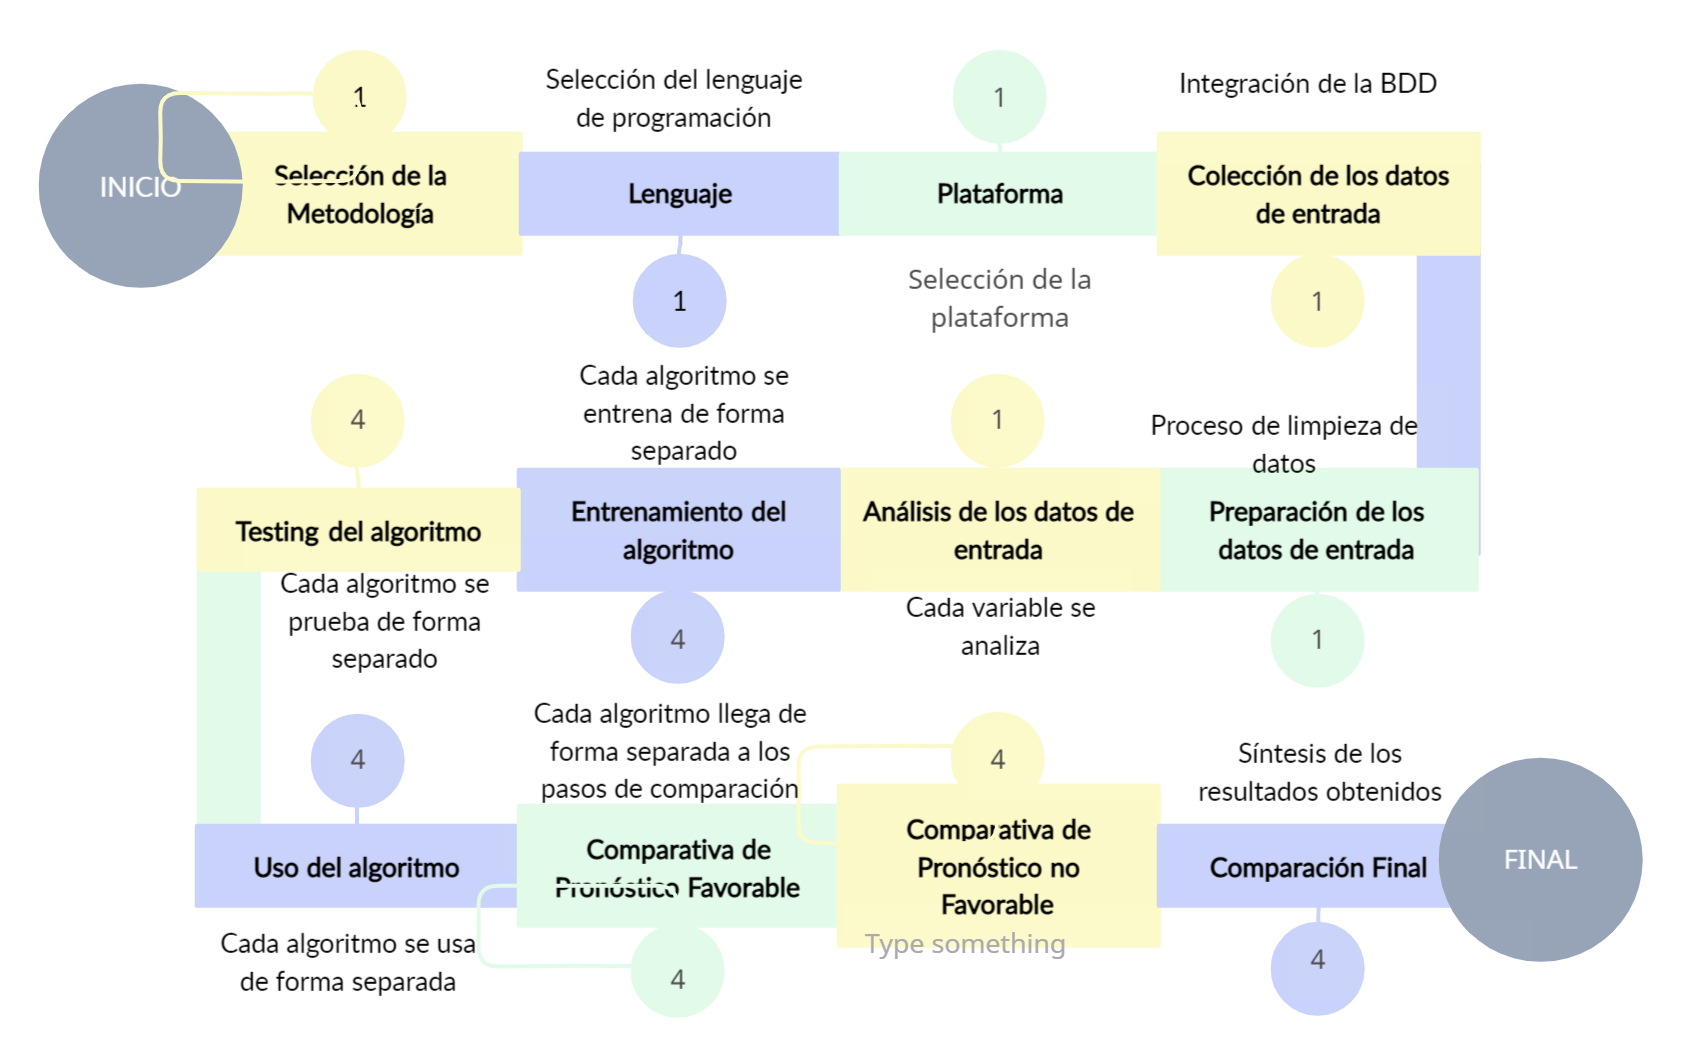
\includegraphics[scale=0.65]{img/mapaDetiempo.png} 
	\caption{Mapa de secuencia metodológica}
	\label{fig:mapaDeTiempo}
\end{figure}


\doublespacing
\subsection{Lenguaje de programación y plataforma}
\spacing{1.5}
Los lenguajes de programación más usados para el ML son Java, R o Python. Para este proyecto se escogió Python por cuatro motivos: 

\begin{enumerate}
	\item Librerías potentes: Python tiene una amplia gama de librerías y frameworks específicos para IA, como TensorFlow, PyTorch, scikit-learn, entre otros, que facilitan la creación y entrenamiento de modelos de IA.
	\item Fácil de aprender: La sintaxis clara y legible de Python hace que sea fácil de aprender y usar para los desarrolladores, lo que significa que se pueden desarrollar modelos de IA de manera más eficiente.
	\item Comunidad activa: La comunidad de Python es activa y colaborativa, lo que significa que hay una gran cantidad de recursos y soluciones disponibles en línea para ayudar a los desarrolladores a resolver cualquier problema que puedan tener.
	\item Interoperabilidad: Python se integra fácilmente con otros lenguajes y tecnologías, lo que significa que se pueden utilizar conjuntamente con otros sistemas y herramientas en proyectos de IA.\\
\end{enumerate}

\par Siguiendo con este razonamiento, para trabajar con el lenguaje Python se puedieron ocupar framework como Tensor Flow, Theano, Amazon Machine Learning, entre otros; al final se opto por la plataforma llamada Jupyter Notebook, popular en la Ciencia de Datos e IA debido a estas ventajas:

\begin{enumerate}
	\item Interfaz interactiva: Jupyter permite a los usuarios ejecutar código en un entorno interactivo y ver los resultados en tiempo real, lo que facilita la exploración y experimentación con datos y modelos de IA.
	\item Documentación integrada: Jupyter permite a los usuarios crear documentos que combinan código, texto, gráficos y otros tipos de contenido multimedia, lo que lo convierte en una excelente opción para la creación de informes y presentaciones de resultados.
	\item Compartir y colaborar: Jupyter permite a los usuarios compartir y colaborar fácilmente en proyectos de IA mediante la creación de notebooks en línea y la posibilidad de trabajar en tiempo real con otros usuarios.
	\item Amplia compatibilidad: Jupyter es compatible con una amplia gama de lenguajes de programación, incluyendo Python, R, Julia, entre otros, lo que significa que los usuarios pueden elegir el lenguaje que mejor se adapte a sus necesidades.\\
\end{enumerate}



     \hypertarget{apliacaciuxf3n-del-muxe9todo}{%
\section{Aplicación}\label{apliacaciuxf3n-del-muxe9todo}}

Para empezar, debemos implementar los pasos sugeridos en la sección 4.2 en el mismo orden que se nos presenta. Los pasos 1, 2 y 3 son comunes para todos los algoritmos, por ende, solo se mostrará una vez en la presente investigación. Al finalizar esta sección se verán los pasos 4, 5 y 6 en cada Algoritmo presentado.

    \hypertarget{colecciuxf3n-de-datos-de-entrada}{%
\section{Colección de datos de
entrada}\label{colecciuxf3n-de-datos-de-entrada}}

El primer paso en el método es la Colección de datos de entrada, en este proceso capturaremos los datos provenientes de la BDD del Hospital Herminda Martín de Chillán y luego diseñaremos un nuevo instrumento.

    \begin{tcolorbox}[breakable, size=fbox, boxrule=1pt, pad at break*=1mm,colback=cellbackground, colframe=cellborder]
\prompt{In}{incolor}{1}{\boxspacing}
\begin{Verbatim}[commandchars=\\\{\}]
\PY{c+c1}{\PYZsh{} Libreria para la manipulación de los datos}
\PY{k+kn}{import} \PY{n+nn}{pandas} \PY{k}{as} \PY{n+nn}{pd}
\PY{k+kn}{import} \PY{n+nn}{numpy} \PY{k}{as} \PY{n+nn}{np}

\PY{c+c1}{\PYZsh{} Leer el dataframe}
\PY{n}{dataframe} \PY{o}{=} \PY{n}{pd}\PY{o}{.}\PY{n}{read\PYZus{}excel}\PY{p}{(}\PY{l+s+s1}{\PYZsq{}}\PY{l+s+s1}{../bdd/bdd\PYZus{}final.xlsx}\PY{l+s+s1}{\PYZsq{}}\PY{p}{)}
\PY{n+nb}{print}\PY{p}{(}\PY{n}{dataframe}\PY{p}{)}
\end{Verbatim}
\end{tcolorbox}

\begin{table}[H]
\centering
\setlength{\tabcolsep}{5pt}
\resizebox{1.0\textwidth}{!}{
	\begin{tabular}{|l|l|l|l|c|l|l|l|l|}
\hline
\multicolumn{1}{|c|}{\textbf{CLAVE}} & \multicolumn{1}{c|}{\textbf{COMUNA}} & \multicolumn{1}{c|}{\textbf{TELEFONOS}} & \multicolumn{1}{c|}{\textbf{EDAD}} & \textbf{...} & \textbf{IL-6   corregida} & \multicolumn{1}{c|}{\textbf{log IL-6}} & \multicolumn{1}{c|}{\textbf{IL-6/VEGF}} & \multicolumn{1}{c|}{\textbf{IL-6/PlGF}} \\ \hline \hline
1 & san carlos &  & 53 & \textbf{...} & 0,156952708 & -0,804 & -0,454839548 & -0,825732298 \\ \hline
2 & coihueco & 41723921-74822219 & 54 & \textbf{...} & 0,012817828 & -1,892 & -0,882899371 & -1,081411325 \\ \hline
3 & chillan & 71818219-50323843 & 78 & \textbf{...} & 0,436365262 & -0,360 & -0,230735564 & -0,296817468 \\ \hline
\multicolumn{1}{|c|}{\textbf{\begin{tabular}[c]{@{}c@{}}.\\ .\\ .\end{tabular}}} & \multicolumn{1}{c|}{\textbf{\begin{tabular}[c]{@{}c@{}}.\\ .\\ .\end{tabular}}} & \multicolumn{1}{c|}{\textbf{\begin{tabular}[c]{@{}c@{}}.\\ .\\ .\end{tabular}}} & \multicolumn{1}{c|}{\textbf{\begin{tabular}[c]{@{}c@{}}.\\ .\\ .\end{tabular}}} & \textbf{...} & \multicolumn{1}{c|}{\textbf{\begin{tabular}[c]{@{}c@{}}.\\ .\\ .\end{tabular}}} & \multicolumn{1}{c|}{\textbf{\begin{tabular}[c]{@{}c@{}}.\\ .\\ .\end{tabular}}} & \multicolumn{1}{c|}{\textbf{\begin{tabular}[c]{@{}c@{}}.\\ .\\ .\end{tabular}}} & \multicolumn{1}{c|}{\textbf{\begin{tabular}[c]{@{}c@{}}.\\ .\\ .\end{tabular}}} \\ \hline
75 & pinto & 82525308 & 79 & \textbf{...} & 0,842328176 & -0,075 & -0,047317636 & -0,08950326 \\ \hline
76 & chillan & 50711724-87107760 & 54 & \textbf{...} & 1,273106319 & 0,105 & 0,054145766 & 0,137865611 \\ \hline
TENS & chillan & 85226191-96473857 & 69 & \textbf{...} & 0,795830574 & -0,099 & \#¡NUM! & \#¡NUM! \\ \hline
\end{tabular}%
}
\caption{Base de datos de pacientes post ACV Isquémico del Hospital Herminda Martin}
\label{tab:bdd}
\end{table}

    \begin{tcolorbox}[breakable, size=fbox, boxrule=1pt, pad at break*=1mm,colback=cellbackground, colframe=cellborder]
\prompt{In}{incolor}{2}{\boxspacing}
\begin{Verbatim}[commandchars=\\\{\}]
\PY{c+c1}{\PYZsh{} Mostramos las variables que posee la base de datos}
\PY{n}{columns\PYZus{}names} \PY{o}{=} \PY{n}{dataframe}\PY{o}{.}\PY{n}{columns}\PY{o}{.}\PY{n}{values}
\PY{n+nb}{print}\PY{p}{(}\PY{n}{columns\PYZus{}names}\PY{p}{)}
\end{Verbatim}
\end{tcolorbox}

    \begin{Verbatim}[commandchars=\\\{\}]
['CLAVE' 'COMUNA' 'TELEFONOS ' 'FICHA CLINICA' 'CTA CTE' 'EDAD' 'PESO'
 'TALLA' 'HTA' 'DIABETES' 'OTRAS PATOLOGIAS' 'FUMA' 'FC' 'PAS' 'PAD'
 'GLUCOSA' 'Hb A/C  \%' 'COL. TOTAL' 'TRIGLICERIDOS' 'LDL' 'HDL' 'HCTO'
 'HB' 'VCM' 'HCM' 'VHS' 'PLAQUETAS' 'INR' 'CONTEO G.B.' 'P.C.R'
 'Nitrogeno Ureico' 'Uremia' 'Creatinina' 'TTPA' 'TP' 'NA' 'K' 'CL'
 'Fosfatasa Alcalina' 'Gamma glutamil' 'Transaminasa piruvica'
 'Trans oxal' 'AREA DE LESION ' 'No  ESTENOSIS INTRACRANEAL'
 'No  ESTENOSIS EXTRACRANEAL' '\%  ESTENOSIS INTRACRANEAL'
 '\%  ESTENOSIS EXTRACRANEAL' 'GLASGOW AL INICO ACV' 'NIHSS INICO ACV'
 'RANKIN INICIO ACV' 'NIHSS alta ACV' 'RANKIN alta ACV' 'NIHSS 6M'
 'RANKIN 6M' 'diag Elopez' 'DIAG. NEUROLOGICO' 'Diag2' 'Diag3'
 'FECHA TOMA MUESTRA' 'Estado paciente' 'Fecha defuncion'
 'CAUSA  DEFUNCION ' 'MOTIVO DE DESCARTE ' 'TROMBOLISIS' 'eduardo'
 'sirve ' 'escala' 'exosomes 1' 'exosomes 2' 'VEGF ab1' 'VEGF ab2'
 'VEGF prome' 'plgf mg prot' 'plgf mg prot.1' 'plgf promedio' 'logVEGF'
 'logPlGF' 'logPCR' 'PCR/VEGF ratio' 'PCR/PLGF ratio' 'IL-6 (pg/ml)'
 'IL-6 corregida' 'log IL-6' 'IL-6/VEGF' 'IL-6/PlGF']
    \end{Verbatim}

    Mostramos la cantidad de pacientes y variables(columnas) que posee la
BDD:

    \begin{tcolorbox}[breakable, size=fbox, boxrule=1pt, pad at break*=1mm,colback=cellbackground, colframe=cellborder]
\prompt{In}{incolor}{3}{\boxspacing}
\begin{Verbatim}[commandchars=\\\{\}]
\PY{n+nb}{print}\PY{p}{(}\PY{l+s+s1}{\PYZsq{}}\PY{l+s+s1}{Existen }\PY{l+s+si}{\PYZob{}\PYZcb{}}\PY{l+s+s1}{ pacientes con }\PY{l+s+si}{\PYZob{}\PYZcb{}}\PY{l+s+s1}{ variables.}\PY{l+s+s1}{\PYZsq{}}\PY{o}{.}\PY{n}{format}\PY{p}{(}\PY{o}{*}\PY{n}{dataframe}\PY{o}{.}\PY{n}{shape}\PY{p}{)}\PY{p}{)}
\PY{n+nb}{print}\PY{p}{(}\PY{l+s+s2}{\PYZdq{}}\PY{l+s+s2}{Existen}\PY{l+s+s2}{\PYZdq{}}\PY{p}{,} \PY{n}{dataframe}\PY{o}{.}\PY{n}{size}\PY{p}{,} \PY{l+s+s2}{\PYZdq{}}\PY{l+s+s2}{elementos}\PY{l+s+s2}{\PYZdq{}}\PY{p}{)}
\end{Verbatim}
\end{tcolorbox}

    \begin{Verbatim}[commandchars=\\\{\}]
Existen 75 pacientes con 85 variables.
Existen 6375 elementos
    \end{Verbatim}

    Se observa que la BDD posee muchas variables y pocos pacientes registrados en las tuplas. Esto hará que sea más difícil la predicción para los algoritmos, así que necesitamos un nuevo instrumento.

    \hypertarget{diseuxf1o-del-instrumento}{%
\subsection{Diseño del instrumento}\label{diseuxf1o-del-instrumento}}

Desde el punto de vista científico, para que un estudio salga lo más certero posible necesitamos variables significativas para la investigación y con la menor pérdida de datos posible. En la BDD todas las variables presentan importancia, algunas son imprescindibles para la investigación, otras con pocos datos completados o simplemente las variables sujetas a interpretación médica (humana). Debido a lo anterior se seleccionaron las variables por dos motivos, el primero fue porque eran las que estaban más completas en la BDD y el segundo porque se determinó que eran más significativas para la investigación por estudios realizados al ACV y dataset presentes en internet. A continuación, se mostrarán las variables escogidas y una pequeña descripción de ellas.

    \begin{quote}
\textbf{HTA}: \texttt{"si"\ o\ "no",\ HIPERTENSIÓN}
\end{quote}

\begin{quote}
\textbf{DIABETES}: \texttt{"si"\ o\ "no"}
\end{quote}

\begin{quote}
\textbf{EDAD}: \texttt{Edad\ del\ paciente}
\end{quote}

\begin{quote}
\textbf{GLUCOSA}: \texttt{Nivel\ de\ azúcar\ en\ la\ sangre}
\end{quote}

\begin{quote}
\textbf{COL. TOTAL}: \texttt{Cantidad\ de\ Colesterol\ en\ la\ sangre}
\end{quote}

\begin{quote}
\textbf{TRIGLICERIDOS}:
\texttt{Cantidad\ de\ triglicéridos\ en\ la\ sangre}
\end{quote}

\begin{quote}
\textbf{INR}:
\texttt{Índice\ internacional\ normalizado\ (INR,\ por\ sus\ siglas\ en\ inglés)\ es\ un\ tipo\ de\ cálculo\ que\ se\ basa\ en\ los\ resultados\ de\ las\ pruebas\ de\ tiempo\ de\ protrombina}
\end{quote}

\begin{quote}
\textbf{CONTEO G.B.}:
\texttt{Conteo\ de\ glóbulos\ blancos\ en\ la\ sangre}
\end{quote}

\begin{quote}
\textbf{GLASGOW AL INICO ACV}:
\texttt{Escala\ de\ 15\ puntos\ médica\ que\ es\ para\ medir\ el\ estado\ de\ conciencia.\ Esta\ pertence\ a\ la\ Inicial}
\end{quote}

\begin{quote}
\textbf{NIHSS INICO ACV}:
\texttt{Escala\ de\ 42\ puntos\ más\ empleada\ para\ la\ valoración\ de\ funciones\ neurológicas\ básicas\ en\ la\ fase\ aguda\ del\ ictus\ isquémico,\ tanto\ al\ inicio\ como\ durante\ su\ evolución.\ Esta\ pertence\ a\ la\ Inicial}
\end{quote}

\begin{quote}
\textbf{NIHSS alta ACV}:
\texttt{Pertenece\ cuando\ es\ dado\ de\ alta\ el\ paciente}
\end{quote}

    La Hipertensión Arterial y la Diabetes son factores de riesgo altos en cualquier enfermedad no trasmisible, por esto son de las primeras seleccionadas, que además contaremos con las escalas de Glasgow y NIHSS que son escalas internacionales para la evaluación del ACV Isquémico.

    \hypertarget{preparaciuxf3n-de-los-datos-de-entrada}{%
\section{Preparación de los datos de
entrada}\label{preparaciuxf3n-de-los-datos-de-entrada}}

El segundo paso descrito en la metodología  es un paso crítico y uno de los más extensos en el desarrollo de proyectos de ML. Aqui se llevará a cabo una limpieza de datos, como la eliminicaión de registros o rescatar datos nulos; selección de caracteristicas que sean relevantes para la investigación; transformación de caracteristicas, que serán para escalar datos para que se adecuen al modelo de ML.

    \hypertarget{eliminaciuxf3n-las-filas-de-los-pacientes-que-se-expulsaron-de-la-bdd}{%
\subsection{Eliminación valores nulos}\label{eliminaciuxf3n-las-filas-de-los-pacientes-que-se-expulsaron-de-la-bdd}}

Como se indicó anteriormente, se dispone de 75 tuplas con 85 columnas, con un total de 6375 elementos, que se planean disminuir por indicación del médico que facilitó la base de datos. La indicación fue que había pacientes que fueron retirados del programa y estaban marcados con un ``out'' en la variable de ``diag Elopez''.

    \begin{tcolorbox}[breakable, size=fbox, boxrule=1pt, pad at break*=1mm,colback=cellbackground, colframe=cellborder]
\prompt{In}{incolor}{4}{\boxspacing}
\begin{Verbatim}[commandchars=\\\{\}]
\PY{n}{dataframe}\PY{o}{.}\PY{n}{drop}\PY{p}{(}\PY{n}{dataframe}\PY{p}{[}\PY{p}{(}\PY{n}{dataframe}\PY{p}{[}\PY{l+s+s1}{\PYZsq{}}\PY{l+s+s1}{diag Elopez}\PY{l+s+s1}{\PYZsq{}}\PY{p}{]} \PY{o}{==} \PY{l+s+s1}{\PYZsq{}}\PY{l+s+s1}{out}\PY{l+s+s1}{\PYZsq{}}\PY{p}{)}\PY{p}{]}\PY{o}{.}\PY{n}{index}\PY{p}{,} \PY{n}{inplace}\PY{o}{=}\PY{k+kc}{True}\PY{p}{)}

\PY{c+c1}{\PYZsh{} mostramos 10 columnas}
\PY{n}{pd}\PY{o}{.}\PY{n}{options}\PY{o}{.}\PY{n}{display}\PY{o}{.}\PY{n}{max\PYZus{}columns} \PY{o}{=} \PY{l+m+mi}{10}

\PY{c+c1}{\PYZsh{} Mostramos las primeras 7 tuplas}
\PY{n}{dataframe}\PY{o}{.}\PY{n}{head}\PY{p}{(}\PY{l+m+mi}{7}\PY{p}{)}
\end{Verbatim}
\end{tcolorbox}

\begin{table}[H]
\centering
\setlength{\tabcolsep}{5pt}
\resizebox{1.0\textwidth}{!}{
	\begin{tabular}{|l|l|l|l|c|l|l|l|l|}
\hline
\multicolumn{1}{|c|}{\textbf{CLAVE}} & \multicolumn{1}{c|}{\textbf{COMUNA}} & \multicolumn{1}{c|}{\textbf{TELEFONOS}} & \multicolumn{1}{c|}{\textbf{EDAD}} & \textbf{...} & \textbf{IL-6   corregida} & \multicolumn{1}{c|}{\textbf{log IL-6}} & \multicolumn{1}{c|}{\textbf{IL-6/VEGF}} & \multicolumn{1}{c|}{\textbf{IL-6/PlGF}} \\ \hline \hline
1 & san carlos &  & 53 & \textbf{...} & 0,156952708 & -0,804 & -0,454839548 & -0,825732298 \\ \hline
2 & coihueco & 41723921-74822219 & 54 & \textbf{...} & 0,012817828 & -1,892 & -0,882899371 & -1,081411325 \\ \hline
3 & chillan & 71818219-50323843 & 78 & \textbf{...} & 0,436365262 & -0,360 & -0,230735564 & -0,296817468 \\ \hline
\multicolumn{1}{|c|}{\textbf{\begin{tabular}[c]{@{}c@{}}.\\ .\\ .\end{tabular}}} & \multicolumn{1}{c|}{\textbf{\begin{tabular}[c]{@{}c@{}}.\\ .\\ .\end{tabular}}} & \multicolumn{1}{c|}{\textbf{\begin{tabular}[c]{@{}c@{}}.\\ .\\ .\end{tabular}}} & \multicolumn{1}{c|}{\textbf{\begin{tabular}[c]{@{}c@{}}.\\ .\\ .\end{tabular}}} & \textbf{...} & \multicolumn{1}{c|}{\textbf{\begin{tabular}[c]{@{}c@{}}.\\ .\\ .\end{tabular}}} & \multicolumn{1}{c|}{\textbf{\begin{tabular}[c]{@{}c@{}}.\\ .\\ .\end{tabular}}} & \multicolumn{1}{c|}{\textbf{\begin{tabular}[c]{@{}c@{}}.\\ .\\ .\end{tabular}}} & \multicolumn{1}{c|}{\textbf{\begin{tabular}[c]{@{}c@{}}.\\ .\\ .\end{tabular}}} \\ \hline
75 & pinto & 82525308 & 79 & \textbf{...} & 0,842328176 & -0,075 & -0,047317636 & -0,08950326 \\ \hline
76 & chillan & 50711724-87107760 & 54 & \textbf{...} & 1,273106319 & 0,105 & 0,054145766 & 0,137865611 \\ \hline
TENS & chillan & 85226191-96473857 & 69 & \textbf{...} & 0,795830574 & -0,099 & \#¡NUM! & \#¡NUM! \\ \hline
\end{tabular}%
}
\caption{Eliminación de pacientes que no aportan en la investigación}
\label{tab:bdd}
\end{table}
        
    \begin{tcolorbox}[breakable, size=fbox, boxrule=1pt, pad at break*=1mm,colback=cellbackground, colframe=cellborder]
\prompt{In}{incolor}{5}{\boxspacing}
\begin{Verbatim}[commandchars=\\\{\}]
\PY{n+nb}{print}\PY{p}{(}\PY{l+s+s1}{\PYZsq{}}\PY{l+s+s1}{Existen }\PY{l+s+si}{\PYZob{}\PYZcb{}}\PY{l+s+s1}{ pacientes con }\PY{l+s+si}{\PYZob{}\PYZcb{}}\PY{l+s+s1}{ variables.}\PY{l+s+s1}{\PYZsq{}}\PY{o}{.}\PY{n}{format}\PY{p}{(}\PY{o}{*}\PY{n}{dataframe}\PY{o}{.}\PY{n}{shape}\PY{p}{)}\PY{p}{)}
\PY{n+nb}{print}\PY{p}{(}\PY{l+s+s2}{\PYZdq{}}\PY{l+s+s2}{Existen}\PY{l+s+s2}{\PYZdq{}}\PY{p}{,} \PY{n}{dataframe}\PY{o}{.}\PY{n}{size}\PY{p}{,} \PY{l+s+s2}{\PYZdq{}}\PY{l+s+s2}{elementos}\PY{l+s+s2}{\PYZdq{}}\PY{p}{)}
\end{Verbatim}
\end{tcolorbox}

    \begin{Verbatim}[commandchars=\\\{\}]
Existen 46 pacientes con 85 variables.
Existen 3910 elementos
    \end{Verbatim}

    \hypertarget{variables-significativas-para-la-investigaciuxf3n}{%
\subsection{Variables significativas para la
investigación}\label{variables-significativas-para-la-investigaciuxf3n}}

Ahora asignamos las variables significativas, para esto se extrae la información del marco de trabajo, identificando las variables categóricas para un arreglo completamente nuevo y así empezar a trabajar sobre el nuevo archivo.

    \begin{tcolorbox}[breakable, size=fbox, boxrule=1pt, pad at break*=1mm,colback=cellbackground, colframe=cellborder]
\prompt{In}{incolor}{6}{\boxspacing}
\begin{Verbatim}[commandchars=\\\{\}]
\PY{c+c1}{\PYZsh{} Tomaremos las variables más significativas para la investigación}
\PY{n}{columnasMuestra} \PY{o}{=} \PY{p}{[}\PY{l+s+s1}{\PYZsq{}}\PY{l+s+s1}{HTA}\PY{l+s+s1}{\PYZsq{}}\PY{p}{,} \PY{l+s+s1}{\PYZsq{}}\PY{l+s+s1}{DIABETES}\PY{l+s+s1}{\PYZsq{}}\PY{p}{,} \PY{l+s+s1}{\PYZsq{}}\PY{l+s+s1}{EDAD}\PY{l+s+s1}{\PYZsq{}}\PY{p}{,} \PY{l+s+s1}{\PYZsq{}}\PY{l+s+s1}{GLUCOSA}\PY{l+s+s1}{\PYZsq{}}\PY{p}{,} \PY{l+s+s1}{\PYZsq{}}\PY{l+s+s1}{COL. TOTAL}\PY{l+s+s1}{\PYZsq{}}\PY{p}{,} \PY{l+s+s1}{\PYZsq{}}\PY{l+s+s1}{TRIGLICERIDOS}\PY{l+s+s1}{\PYZsq{}}\PY{p}{,} \PY{l+s+s1}{\PYZsq{}}\PY{l+s+s1}{INR}\PY{l+s+s1}{\PYZsq{}}\PY{p}{,} \PY{l+s+s1}{\PYZsq{}}\PY{l+s+s1}{CONTEO G.B.}\PY{l+s+s1}{\PYZsq{}}\PY{p}{,} \PY{l+s+s1}{\PYZsq{}}\PY{l+s+s1}{GLASGOW AL INICO ACV}\PY{l+s+s1}{\PYZsq{}}\PY{p}{,} \PY{l+s+s1}{\PYZsq{}}\PY{l+s+s1}{NIHSS INICO ACV}\PY{l+s+s1}{\PYZsq{}}\PY{p}{,} \PY{l+s+s1}{\PYZsq{}}\PY{l+s+s1}{NIHSS alta ACV}\PY{l+s+s1}{\PYZsq{}}\PY{p}{]}
\PY{n}{dataset} \PY{o}{=} \PY{n}{dataframe}\PY{p}{[}\PY{p}{[}\PY{o}{*}\PY{n}{columnasMuestra}\PY{p}{]}\PY{p}{]}

\PY{c+c1}{\PYZsh{} Muestramos las columnas que se ajusten a la cantidad de espacio}
\PY{n}{pd}\PY{o}{.}\PY{n}{options}\PY{o}{.}\PY{n}{display}\PY{o}{.}\PY{n}{max\PYZus{}columns} \PY{o}{=} \PY{l+m+mi}{0}

\PY{n}{dataset}\PY{o}{.}\PY{n}{head}\PY{p}{(}\PY{l+m+mi}{5}\PY{p}{)}
\end{Verbatim}
\end{tcolorbox}

\begin{table}[H]
\centering
\setlength{\tabcolsep}{5pt}
\resizebox{1.0\textwidth}{!}{
\begin{tabular}{|l|l|l|l|l|l|l|l|l|l|l|}
\hline
\multicolumn{1}{|c|}{\textbf{HTA}} & \multicolumn{1}{c|}{\textbf{DIABETES}} & \multicolumn{1}{c|}{\textbf{EDAD}} & \multicolumn{1}{c|}{\textbf{GLUCOSA}} & \multicolumn{1}{c|}{\textbf{COL. TOTAL}} & \multicolumn{1}{c|}{\textbf{TRIGLICERIDOS}} & \multicolumn{1}{c|}{\textbf{INR}} & \multicolumn{1}{c|}{\textbf{CONTEO G.B.}} & \multicolumn{1}{c|}{\textbf{GLASGOW AL INICO   ACV}} & \multicolumn{1}{c|}{\textbf{NIHSS INICO ACV}} & \multicolumn{1}{c|}{\textbf{NIHSS alta ACV}} \\ \hline \hline
 &  & 53 & 137,09 & 268 & 130 & 1,08 & 41,9 & 11 & 14 & 42 \\ \hline
si & si & 54 &  & 187 & 130 &  & 8,3 & 15 & 6 & 0 \\ \hline
si & si & 78 & 359,42 & 159 & 97 & 0,89 & 8,5 & 15 & 5 & 2 \\ \hline
\multicolumn{1}{|c|}{\textbf{\begin{tabular}[c]{@{}c@{}}.\\ .\\ .\end{tabular}}} & \multicolumn{1}{c|}{\textbf{\begin{tabular}[c]{@{}c@{}}.\\ .\\ .\end{tabular}}} & \multicolumn{1}{c|}{\textbf{\begin{tabular}[c]{@{}c@{}}.\\ .\\ .\end{tabular}}} & \multicolumn{1}{c|}{\textbf{\begin{tabular}[c]{@{}c@{}}.\\ .\\ .\end{tabular}}} & \multicolumn{1}{c|}{\textbf{\begin{tabular}[c]{@{}c@{}}.\\ .\\ .\end{tabular}}} & \multicolumn{1}{c|}{\textbf{\begin{tabular}[c]{@{}c@{}}.\\ .\\ .\end{tabular}}} & \multicolumn{1}{c|}{\textbf{\begin{tabular}[c]{@{}c@{}}.\\ .\\ .\end{tabular}}} & \multicolumn{1}{c|}{\textbf{\begin{tabular}[c]{@{}c@{}}.\\ .\\ .\end{tabular}}} & \multicolumn{1}{c|}{\textbf{\begin{tabular}[c]{@{}c@{}}.\\ .\\ .\end{tabular}}} & \multicolumn{1}{c|}{\textbf{\begin{tabular}[c]{@{}c@{}}.\\ .\\ .\end{tabular}}} & \multicolumn{1}{c|}{\textbf{\begin{tabular}[c]{@{}c@{}}.\\ .\\ .\end{tabular}}} \\ \hline
si & si & 79 & 116,99 & 109 & 118 &  & 9,9 &  & 2 & 2 \\ \hline
si & si & 54 & 211,58 &  &  & 0,99 & 6,5 & 15 & 1 & 1 \\ \hline
si & si & 69 & 217,21 & 202 & 232 & 1,03 & 10,4 & 0 &  &  \\ \hline
\end{tabular}%
}
\caption{Dataset de variables para la investigación}
\label{tab:dataset}
\end{table}
        
    Mostramos la cantidad de pacientes y variables/columnas que posee la BDD después de la selección de variables significativas para la investigación:

    \begin{tcolorbox}[breakable, size=fbox, boxrule=1pt, pad at break*=1mm,colback=cellbackground, colframe=cellborder]
\prompt{In}{incolor}{7}{\boxspacing}
\begin{Verbatim}[commandchars=\\\{\}]
\PY{n+nb}{print}\PY{p}{(}\PY{l+s+s1}{\PYZsq{}}\PY{l+s+s1}{Existen }\PY{l+s+si}{\PYZob{}\PYZcb{}}\PY{l+s+s1}{ pacientes con }\PY{l+s+si}{\PYZob{}\PYZcb{}}\PY{l+s+s1}{ variables.}\PY{l+s+s1}{\PYZsq{}}\PY{o}{.}\PY{n}{format}\PY{p}{(}\PY{o}{*}\PY{n}{dataset}\PY{o}{.}\PY{n}{shape}\PY{p}{)}\PY{p}{)}
\PY{n+nb}{print}\PY{p}{(}\PY{l+s+s2}{\PYZdq{}}\PY{l+s+s2}{Existen}\PY{l+s+s2}{\PYZdq{}}\PY{p}{,} \PY{n}{dataset}\PY{o}{.}\PY{n}{size}\PY{p}{,} \PY{l+s+s2}{\PYZdq{}}\PY{l+s+s2}{elementos}\PY{l+s+s2}{\PYZdq{}}\PY{p}{)}
\end{Verbatim}
\end{tcolorbox}

    \begin{Verbatim}[commandchars=\\\{\}]
Existen 46 pacientes con 11 variables.
Existen 506 elementos
    \end{Verbatim}

    \hypertarget{descripciuxf3n-general-de-los-datos}{%
\subsection{Descripción general de los
datos}\label{descripciuxf3n-general-de-los-datos}}

En la descripción de los datos, se muestran parámetros, pérdida de datos (Missing Data), forma y su descripción estadística.

    \begin{tcolorbox}[breakable, size=fbox, boxrule=1pt, pad at break*=1mm,colback=cellbackground, colframe=cellborder]
\prompt{In}{incolor}{8}{\boxspacing}
\begin{Verbatim}[commandchars=\\\{\}]
\PY{c+c1}{\PYZsh{} Check Dataset:}
\PY{k}{def} \PY{n+nf}{check\PYZus{}data}\PY{p}{(}\PY{n}{dataset}\PY{p}{,}\PY{n}{head}\PY{o}{=}\PY{l+m+mi}{5}\PY{p}{)}\PY{p}{:}
    \PY{n+nb}{print}\PY{p}{(}\PY{l+m+mi}{20}\PY{o}{*}\PY{l+s+s2}{\PYZdq{}}\PY{l+s+s2}{\PYZhy{}}\PY{l+s+s2}{\PYZdq{}} \PY{o}{+} \PY{l+s+s2}{\PYZdq{}}\PY{l+s+s2}{Información}\PY{l+s+s2}{\PYZdq{}}\PY{o}{.}\PY{n}{center}\PY{p}{(}\PY{l+m+mi}{20}\PY{p}{)} \PY{o}{+} \PY{l+m+mi}{20}\PY{o}{*}\PY{l+s+s2}{\PYZdq{}}\PY{l+s+s2}{\PYZhy{}}\PY{l+s+s2}{\PYZdq{}}\PY{p}{)}
    \PY{n+nb}{print}\PY{p}{(}\PY{n}{dataset}\PY{o}{.}\PY{n}{info}\PY{p}{(}\PY{p}{)}\PY{p}{)}
    \PY{n+nb}{print}\PY{p}{(}\PY{l+m+mi}{20}\PY{o}{*}\PY{l+s+s2}{\PYZdq{}}\PY{l+s+s2}{\PYZhy{}}\PY{l+s+s2}{\PYZdq{}} \PY{o}{+} \PY{l+s+s2}{\PYZdq{}}\PY{l+s+s2}{Forma de datos}\PY{l+s+s2}{\PYZdq{}}\PY{o}{.}\PY{n}{center}\PY{p}{(}\PY{l+m+mi}{20}\PY{p}{)} \PY{o}{+} \PY{l+m+mi}{20}\PY{o}{*}\PY{l+s+s2}{\PYZdq{}}\PY{l+s+s2}{\PYZhy{}}\PY{l+s+s2}{\PYZdq{}}\PY{p}{)}
    \PY{n+nb}{print}\PY{p}{(}\PY{n}{dataset}\PY{o}{.}\PY{n}{shape}\PY{p}{)}
    \PY{n+nb}{print}\PY{p}{(}\PY{l+s+s2}{\PYZdq{}}\PY{l+s+se}{\PYZbs{}n}\PY{l+s+s2}{\PYZdq{}} \PY{o}{+} \PY{l+m+mi}{20}\PY{o}{*}\PY{l+s+s2}{\PYZdq{}}\PY{l+s+s2}{\PYZhy{}}\PY{l+s+s2}{\PYZdq{}} \PY{o}{+} \PY{l+s+s2}{\PYZdq{}}\PY{l+s+s2}{Los primeros 5 datos}\PY{l+s+s2}{\PYZdq{}}\PY{o}{.}\PY{n}{center}\PY{p}{(}\PY{l+m+mi}{20}\PY{p}{)} \PY{o}{+} \PY{l+m+mi}{20}\PY{o}{*}\PY{l+s+s2}{\PYZdq{}}\PY{l+s+s2}{\PYZhy{}}\PY{l+s+s2}{\PYZdq{}}\PY{p}{)}
    \PY{n+nb}{print}\PY{p}{(}\PY{n}{dataset}\PY{o}{.}\PY{n}{head}\PY{p}{(}\PY{p}{)}\PY{p}{)}
    \PY{n+nb}{print}\PY{p}{(}\PY{l+s+s2}{\PYZdq{}}\PY{l+s+se}{\PYZbs{}n}\PY{l+s+s2}{\PYZdq{}} \PY{o}{+} \PY{l+m+mi}{20} \PY{o}{*} \PY{l+s+s2}{\PYZdq{}}\PY{l+s+s2}{\PYZhy{}}\PY{l+s+s2}{\PYZdq{}} \PY{o}{+} \PY{l+s+s2}{\PYZdq{}}\PY{l+s+s2}{Los últimos 5 datos}\PY{l+s+s2}{\PYZdq{}}\PY{o}{.}\PY{n}{center}\PY{p}{(}\PY{l+m+mi}{20}\PY{p}{)} \PY{o}{+} \PY{l+m+mi}{20} \PY{o}{*} \PY{l+s+s2}{\PYZdq{}}\PY{l+s+s2}{\PYZhy{}}\PY{l+s+s2}{\PYZdq{}}\PY{p}{)}
    \PY{n+nb}{print}\PY{p}{(}\PY{n}{dataset}\PY{o}{.}\PY{n}{tail}\PY{p}{(}\PY{p}{)}\PY{p}{)}
    \PY{n+nb}{print}\PY{p}{(}\PY{l+s+s2}{\PYZdq{}}\PY{l+s+se}{\PYZbs{}n}\PY{l+s+s2}{\PYZdq{}} \PY{o}{+} \PY{l+m+mi}{20} \PY{o}{*} \PY{l+s+s2}{\PYZdq{}}\PY{l+s+s2}{\PYZhy{}}\PY{l+s+s2}{\PYZdq{}} \PY{o}{+} \PY{l+s+s2}{\PYZdq{}}\PY{l+s+s2}{Missing Data}\PY{l+s+s2}{\PYZdq{}}\PY{o}{.}\PY{n}{center}\PY{p}{(}\PY{l+m+mi}{20}\PY{p}{)} \PY{o}{+} \PY{l+m+mi}{20} \PY{o}{*} \PY{l+s+s2}{\PYZdq{}}\PY{l+s+s2}{\PYZhy{}}\PY{l+s+s2}{\PYZdq{}}\PY{p}{)}
    \PY{n+nb}{print}\PY{p}{(}\PY{n}{dataset}\PY{o}{.}\PY{n}{isnull}\PY{p}{(}\PY{p}{)}\PY{o}{.}\PY{n}{sum}\PY{p}{(}\PY{p}{)}\PY{p}{)}
    \PY{n+nb}{print}\PY{p}{(}\PY{l+s+s2}{\PYZdq{}}\PY{l+s+se}{\PYZbs{}n}\PY{l+s+s2}{\PYZdq{}} \PY{o}{+} \PY{l+m+mi}{20} \PY{o}{*} \PY{l+s+s2}{\PYZdq{}}\PY{l+s+s2}{\PYZhy{}}\PY{l+s+s2}{\PYZdq{}} \PY{o}{+} \PY{l+s+s2}{\PYZdq{}}\PY{l+s+s2}{Describir los datos}\PY{l+s+s2}{\PYZdq{}}\PY{o}{.}\PY{n}{center}\PY{p}{(}\PY{l+m+mi}{20}\PY{p}{)} \PY{o}{+} \PY{l+m+mi}{20} \PY{o}{*} \PY{l+s+s2}{\PYZdq{}}\PY{l+s+s2}{\PYZhy{}}\PY{l+s+s2}{\PYZdq{}}\PY{p}{)}
    \PY{n+nb}{print}\PY{p}{(}\PY{n}{dataset}\PY{o}{.}\PY{n}{describe}\PY{p}{(}\PY{p}{)}\PY{o}{.}\PY{n}{T}\PY{p}{)}
\PY{n}{check\PYZus{}data}\PY{p}{(}\PY{n}{dataset}\PY{p}{)}
\end{Verbatim}
\end{tcolorbox}

    \begin{Verbatim}[commandchars=\\\{\}]
--------------------    Información     --------------------
<class 'pandas.core.frame.DataFrame'>
Int64Index: 46 entries, 0 to 74
Data columns (total 11 columns):
 \#   Column                Non-Null Count  Dtype
---  ------                --------------  -----
 0   HTA                   42 non-null     object
 1   DIABETES              34 non-null     object
 2   EDAD                  44 non-null     float64
 3   GLUCOSA               38 non-null     float64
 4   COL. TOTAL            40 non-null     float64
 5   TRIGLICERIDOS         40 non-null     float64
 6   INR                   37 non-null     float64
 7   CONTEO G.B.           46 non-null     float64
 8   GLASGOW AL INICO ACV  29 non-null     float64
 9   NIHSS INICO ACV       39 non-null     float64
 10  NIHSS alta ACV        32 non-null     float64
dtypes: float64(9), object(2)
memory usage: 4.3+ KB
None
--------------------   Forma de datos   --------------------
(46, 11)

--------------------Los primeros 5 datos--------------------
   HTA DIABETES  {\ldots}  NIHSS INICO ACV  NIHSS alta ACV
0  NaN      NaN  {\ldots}             14.0            42.0
1   si       si  {\ldots}              6.0             0.0
2   si       si  {\ldots}              5.0             2.0
3   si       si  {\ldots}              1.0             0.0
4   si       si  {\ldots}              3.0             2.0

[5 rows x 11 columns]

--------------------Los últimos 5 datos --------------------
   HTA DIABETES  {\ldots}  NIHSS INICO ACV  NIHSS alta ACV
68  si       no  {\ldots}              NaN             NaN
69  no       no  {\ldots}              2.0             0.0
72  si       si  {\ldots}              2.0             2.0
73  si       si  {\ldots}              1.0             1.0
74  si       si  {\ldots}              NaN             NaN

[5 rows x 11 columns]

--------------------    Missing Data    --------------------
HTA                      4
DIABETES                12
EDAD                     2
GLUCOSA                  8
COL. TOTAL               6
TRIGLICERIDOS            6
INR                      9
CONTEO G.B.              0
GLASGOW AL INICO ACV    17
NIHSS INICO ACV          7
NIHSS alta ACV          14
dtype: int64

--------------------Describir los datos --------------------
                      count        mean  {\ldots}       75\%     max
EDAD                   44.0   71.522727  {\ldots}   80.5000   90.00
GLUCOSA                38.0  135.529211  {\ldots}  162.5925  359.42
COL. TOTAL             40.0  162.750000  {\ldots}  188.5000  342.00
TRIGLICERIDOS          40.0  123.450000  {\ldots}  142.0000  232.00
INR                    37.0    1.197568  {\ldots}    1.2000    3.08
CONTEO G.B.            46.0   10.119783  {\ldots}   10.3750   41.90
GLASGOW AL INICO ACV   29.0   13.482759  {\ldots}   15.0000   15.00
NIHSS INICO ACV        39.0    5.564103  {\ldots}    6.5000   21.00
NIHSS alta ACV         32.0    5.687500  {\ldots}    4.0000   42.00

[9 rows x 8 columns]
    \end{Verbatim}

    La descripción de los datos nos ayuda a evaluar los casos particulares de las variables que serán tratadas en los siguientes títulos.

    \hypertarget{missing-data}{%
\subsection{Missing data}\label{missing-data}}

Los datos que faltan ocurren cuando no se almacena ningún valor en la variable de observación. Aunque el Missing data es una ocurrencia muy común, estos pueden tener una presión significativa en los resultados de la aplicación del instrumento. Para corregir este problema, existen variadas técnicas estadísticas, siendo una de ellas la mediana y el redondeo como lo muestra \cite{Bar2017} en algunas variables que utilizaremos para llenar las celdas faltantes. Tomaremos la información que mostramos anteriormente.

    \begin{tcolorbox}[breakable, size=fbox, boxrule=1pt, pad at break*=1mm,colback=cellbackground, colframe=cellborder]
\prompt{In}{incolor}{9}{\boxspacing}
\begin{Verbatim}[commandchars=\\\{\}]
\PY{n}{dataset}\PY{o}{.}\PY{n}{isnull}\PY{p}{(}\PY{p}{)}\PY{o}{.}\PY{n}{sum}\PY{p}{(}\PY{p}{)}
\end{Verbatim}
\end{tcolorbox}

\begin{table}[H]
\centering
\setlength{\tabcolsep}{5pt}
\resizebox{0.5\textwidth}{!}{
	\begin{tabular}{|r|r|}
\hline
\multicolumn{1}{|l|}{\textbf{}} & \multicolumn{1}{c|}{\textbf{MISSING DATA}} \\ \hline \hline
\textbf{HTA } & 4 \\ \hline
\textbf{DIABETES } & 12 \\ \hline
\textbf{EDAD } & 2 \\ \hline
\textbf{GLUCOSA } & 8 \\ \hline
\textbf{COL. TOTAL } & 6 \\ \hline
\textbf{TRIGLICERIDOS } & 6 \\ \hline
\textbf{INR } & 9 \\ \hline
\textbf{CONTEO G.B. } & 0 \\ \hline
\textbf{ GLASGOW AL INICO ACV } & 17 \\ \hline
\textbf{NIHSS INICO ACV } & 7 \\ \hline
\textbf{NIHSS alta ACV } & 14 \\ \hline
\end{tabular}%
}
\caption{Missing data de variables}
\label{tab:missing data}
\end{table}
        
    Como se demuestra en la tabla \ref{tab:missing data}, casi todas las variables hay missing data, así que el algoritmo para trabajar será el siguiente:

    \begin{tcolorbox}[breakable, size=fbox, boxrule=1pt, pad at break*=1mm,colback=cellbackground, colframe=cellborder]
\prompt{In}{incolor}{10}{\boxspacing}
\begin{Verbatim}[commandchars=\\\{\}]
\PY{n}{valores\PYZus{}por\PYZus{}defecto} \PY{o}{=} \PY{p}{\PYZob{}}
                       \PY{l+s+s1}{\PYZsq{}}\PY{l+s+s1}{HTA}\PY{l+s+s1}{\PYZsq{}}\PY{p}{:} \PY{l+s+s2}{\PYZdq{}}\PY{l+s+s2}{DESCONOCIDO}\PY{l+s+s2}{\PYZdq{}}\PY{p}{,}
                       \PY{l+s+s1}{\PYZsq{}}\PY{l+s+s1}{DIABETES}\PY{l+s+s1}{\PYZsq{}} \PY{p}{:} \PY{l+s+s2}{\PYZdq{}}\PY{l+s+s2}{DESCONOCIDO}\PY{l+s+s2}{\PYZdq{}}\PY{p}{,}
                       \PY{l+s+s1}{\PYZsq{}}\PY{l+s+s1}{EDAD}\PY{l+s+s1}{\PYZsq{}}\PY{p}{:}\PY{n}{dataset}\PY{p}{[}\PY{l+s+s2}{\PYZdq{}}\PY{l+s+s2}{EDAD}\PY{l+s+s2}{\PYZdq{}}\PY{p}{]}\PY{o}{.}\PY{n}{median}\PY{p}{(}\PY{p}{)}\PY{o}{.}\PY{n}{round}\PY{p}{(}\PY{p}{)}\PY{p}{,}
                       \PY{l+s+s1}{\PYZsq{}}\PY{l+s+s1}{GLUCOSA}\PY{l+s+s1}{\PYZsq{}}\PY{p}{:}\PY{n}{dataset}\PY{p}{[}\PY{l+s+s2}{\PYZdq{}}\PY{l+s+s2}{GLUCOSA}\PY{l+s+s2}{\PYZdq{}}\PY{p}{]}\PY{o}{.}\PY{n}{median}\PY{p}{(}\PY{p}{)}\PY{p}{,}
                       \PY{l+s+s1}{\PYZsq{}}\PY{l+s+s1}{COL. TOTAL}\PY{l+s+s1}{\PYZsq{}}\PY{p}{:}\PY{n}{dataset}\PY{p}{[}\PY{l+s+s2}{\PYZdq{}}\PY{l+s+s2}{COL. TOTAL}\PY{l+s+s2}{\PYZdq{}}\PY{p}{]}\PY{o}{.}\PY{n}{median}\PY{p}{(}\PY{p}{)}\PY{p}{,} 
                       \PY{l+s+s1}{\PYZsq{}}\PY{l+s+s1}{TRIGLICERIDOS}\PY{l+s+s1}{\PYZsq{}}\PY{p}{:}\PY{n}{dataset}\PY{p}{[}\PY{l+s+s2}{\PYZdq{}}\PY{l+s+s2}{TRIGLICERIDOS}\PY{l+s+s2}{\PYZdq{}}\PY{p}{]}\PY{o}{.}\PY{n}{median}\PY{p}{(}\PY{p}{)}\PY{p}{,}
                       \PY{l+s+s1}{\PYZsq{}}\PY{l+s+s1}{INR}\PY{l+s+s1}{\PYZsq{}}\PY{p}{:}\PY{n}{dataset}\PY{p}{[}\PY{l+s+s2}{\PYZdq{}}\PY{l+s+s2}{INR}\PY{l+s+s2}{\PYZdq{}}\PY{p}{]}\PY{o}{.}\PY{n}{median}\PY{p}{(}\PY{p}{)}\PY{p}{,}
                       \PY{l+s+s1}{\PYZsq{}}\PY{l+s+s1}{GLASGOW AL INICO ACV}\PY{l+s+s1}{\PYZsq{}}\PY{p}{:}\PY{n}{dataset}\PY{p}{[}\PY{l+s+s2}{\PYZdq{}}\PY{l+s+s2}{GLASGOW AL INICO ACV}\PY{l+s+s2}{\PYZdq{}}\PY{p}{]}\PY{o}{.}\PY{n}{median}\PY{p}{(}\PY{p}{)}\PY{o}{.}\PY{n}{round}\PY{p}{(}\PY{p}{)}\PY{p}{,}
                       \PY{l+s+s1}{\PYZsq{}}\PY{l+s+s1}{NIHSS INICO ACV}\PY{l+s+s1}{\PYZsq{}}\PY{p}{:}\PY{n}{dataset}\PY{p}{[}\PY{l+s+s2}{\PYZdq{}}\PY{l+s+s2}{NIHSS INICO ACV}\PY{l+s+s2}{\PYZdq{}}\PY{p}{]}\PY{o}{.}\PY{n}{median}\PY{p}{(}\PY{p}{)}\PY{o}{.}\PY{n}{round}\PY{p}{(}\PY{p}{)}\PY{p}{,} 
                       \PY{l+s+s1}{\PYZsq{}}\PY{l+s+s1}{NIHSS alta ACV}\PY{l+s+s1}{\PYZsq{}}\PY{p}{:}\PY{n}{dataset}\PY{p}{[}\PY{l+s+s2}{\PYZdq{}}\PY{l+s+s2}{NIHSS alta ACV}\PY{l+s+s2}{\PYZdq{}}\PY{p}{]}\PY{o}{.}\PY{n}{median}\PY{p}{(}\PY{p}{)}\PY{o}{.}\PY{n}{round}\PY{p}{(}\PY{p}{)}\PY{p}{,} 
                      \PY{p}{\PYZcb{}}
\PY{c+c1}{\PYZsh{} Missing Data}
\PY{n}{dataset} \PY{o}{=} \PY{n}{dataset}\PY{o}{.}\PY{n}{fillna}\PY{p}{(}\PY{n}{value}\PY{o}{=}\PY{n}{valores\PYZus{}por\PYZus{}defecto}\PY{p}{)}
\end{Verbatim}
\end{tcolorbox}

    Comprobamos si ahora existe missing data:

    \begin{tcolorbox}[breakable, size=fbox, boxrule=1pt, pad at break*=1mm,colback=cellbackground, colframe=cellborder]
\prompt{In}{incolor}{11}{\boxspacing}
\begin{Verbatim}[commandchars=\\\{\}]
\PY{n}{dataset}\PY{o}{.}\PY{n}{isnull}\PY{p}{(}\PY{p}{)}\PY{o}{.}\PY{n}{sum}\PY{p}{(}\PY{p}{)}
\end{Verbatim}
\end{tcolorbox}

 \begin{table}[H]
\centering
\setlength{\tabcolsep}{5pt}
\resizebox{0.5\textwidth}{!}{
\begin{tabular}{|r|r|}
\hline
\multicolumn{1}{|l|}{\textbf{}} & \multicolumn{1}{c|}{\textbf{MISSING DATA}} \\ \hline \hline
\textbf{HTA} & 0 \\ \hline
\textbf{DIABETES} & 0 \\ \hline
\textbf{EDAD} & 0 \\ \hline
\textbf{GLUCOSA} & 0 \\ \hline
\textbf{COL. TOTAL} & 0 \\ \hline
\textbf{TRIGLICERIDOS} & 0 \\ \hline
\textbf{INR} & 0 \\ \hline
\textbf{CONTEO G.B.} & 0 \\ \hline
\textbf{GLASGOW AL INICO ACV} & 0 \\ \hline
\textbf{NIHSS INICO ACV} & 0 \\ \hline
\textbf{NIHSS alta ACV} & 0 \\ \hline
\end{tabular}%
}
\caption{Missing data finalizado}
\label{tab:missing data finalizado}
\end{table}
        
    Como se ve en la tabla \ref{tab:missing data finalizado}, ya no existe missing data.

    \hypertarget{preprocesamiento-de-los-datos-y-clasificaciuxf3n}{%
\subsection{Preprocesamiento de los datos y clasificación}\label{preprocesamiento-de-los-datos-y-clasificaciuxf3n}}

La preparación de los datos para el modelo de ML es lo que nos llevará a decidir qué modelo podremos utilizar, ya que trabajar con modelos de clasificación no es lo mismo que con los de regresión. Los pasos exactos para la preparación de los datos dependerán del modelo utilizado y de los datos recopilados.Cabe destacar que se requerirá cierta cantidad de manipulación de datos para cualquier aplicación de ML.

    \hypertarget{anuxe1lisis-de-variable-objetivo}{%
\subsubsection{Análisis de variable Objetivo}\label{anuxe1lisis-de-variable-objetivo}}

	En el apartado del Marco Teórico \ref{sec:NIHSS} se hablo de la escala NIHSS y sus niveles de daño neurológico, considerándola como esta es la variable más importante en la predicción. Dentro de nuestro dataset existe la escala NIHSS al iniciar el ACV, la escala NIHSS al alta del paciente y la escala NIHSS en el control de los 6 meses después del ACV.
\par La escala en la predicción que se utilizará es la escala NIHSS de alta, para poder tener un aseguramiento de la predicción del estado de salud del pacientes a través del camino de salida del hospital, esto quiere decir, conoceremos el estado del paciente al salir de alta y según las demás variables, existe una tendencia para la predicción en la escala NIHSS del alta.

    \begin{tcolorbox}[breakable, size=fbox, boxrule=1pt, pad at break*=1mm,colback=cellbackground, colframe=cellborder]
\prompt{In}{incolor}{12}{\boxspacing}
\begin{Verbatim}[commandchars=\\\{\}]
\PY{n}{dataset}\PY{p}{[}\PY{l+s+s2}{\PYZdq{}}\PY{l+s+s2}{NIHSS alta ACV}\PY{l+s+s2}{\PYZdq{}}\PY{p}{]}\PY{o}{.}\PY{n}{value\PYZus{}counts}\PY{p}{(}\PY{p}{)}
\end{Verbatim}
\end{tcolorbox}

\begin{table}[H]
\centering
\setlength{\tabcolsep}{5pt}
\resizebox{0.4\textwidth}{!}{
	\begin{tabular}{|c|l|}
\hline
\textbf{NIHSS alta ACV} & \multicolumn{1}{c|}{\textbf{Cantidad}} \\ \hline  \hline
\textbf{1} & 19 \\ \hline
\textbf{0} & 12 \\ \hline
\textbf{2} & 6 \\ \hline
\textbf{42} & 2 \\ \hline
\textbf{4} & 2 \\ \hline
\textbf{8} & 1 \\ \hline
\textbf{10} & 1 \\ \hline
\textbf{18} & 1 \\ \hline
\textbf{32} & 1 \\ \hline
\textbf{5} & 1 \\ \hline
\end{tabular}%
}
\caption{Cantidad de pacientes en la escala NIHSS en alta}
\label{tab:nihss alta}
\end{table}
        
    En esta escala los valores menores suponen un mejor pronóstico para los pacientes, es por eso que se decide crear una variable con los resultados que da el test NIHSS.

    \hypertarget{crear-columna-para-nihss_alta_cat}{%
\paragraph{Crear columna para NIHSS\_alta\_cat}\label{crear-columna-para-nihss_alta_cat}}

	Esta columna nos servirá para la clasificación de los estados de la variable NIHSS.

    \begin{tcolorbox}[breakable, size=fbox, boxrule=1pt, pad at break*=1mm,colback=cellbackground, colframe=cellborder]
\prompt{In}{incolor}{13}{\boxspacing}
\begin{Verbatim}[commandchars=\\\{\}]
\PY{c+c1}{\PYZsh{} Realizamos la clasificación de la escala}
\PY{n}{condicionesALTA} \PY{o}{=} \PY{p}{[}
    \PY{p}{(}\PY{n}{dataset}\PY{p}{[}\PY{l+s+s1}{\PYZsq{}}\PY{l+s+s1}{NIHSS alta ACV}\PY{l+s+s1}{\PYZsq{}}\PY{p}{]} \PY{o}{==} \PY{l+m+mi}{0}\PY{p}{)}\PY{p}{,}
    \PY{p}{(}\PY{n}{dataset}\PY{p}{[}\PY{l+s+s1}{\PYZsq{}}\PY{l+s+s1}{NIHSS alta ACV}\PY{l+s+s1}{\PYZsq{}}\PY{p}{]} \PY{o}{==} \PY{l+m+mi}{1}\PY{p}{)}\PY{p}{,}
    \PY{p}{(}\PY{n}{dataset}\PY{p}{[}\PY{l+s+s1}{\PYZsq{}}\PY{l+s+s1}{NIHSS alta ACV}\PY{l+s+s1}{\PYZsq{}}\PY{p}{]} \PY{o}{\PYZgt{}}\PY{o}{=} \PY{l+m+mi}{2}\PY{p}{)} \PY{o}{\PYZam{}} \PY{p}{(}\PY{n}{dataset}\PY{p}{[}\PY{l+s+s1}{\PYZsq{}}\PY{l+s+s1}{NIHSS alta ACV}\PY{l+s+s1}{\PYZsq{}}\PY{p}{]} \PY{o}{\PYZlt{}}\PY{o}{=} \PY{l+m+mi}{5}\PY{p}{)}\PY{p}{,}
    \PY{p}{(}\PY{n}{dataset}\PY{p}{[}\PY{l+s+s1}{\PYZsq{}}\PY{l+s+s1}{NIHSS alta ACV}\PY{l+s+s1}{\PYZsq{}}\PY{p}{]} \PY{o}{\PYZgt{}}\PY{o}{=} \PY{l+m+mi}{6}\PY{p}{)} \PY{o}{\PYZam{}} \PY{p}{(}\PY{n}{dataset}\PY{p}{[}\PY{l+s+s1}{\PYZsq{}}\PY{l+s+s1}{NIHSS alta ACV}\PY{l+s+s1}{\PYZsq{}}\PY{p}{]} \PY{o}{\PYZlt{}}\PY{o}{=} \PY{l+m+mi}{15}\PY{p}{)}\PY{p}{,}
    \PY{p}{(}\PY{n}{dataset}\PY{p}{[}\PY{l+s+s1}{\PYZsq{}}\PY{l+s+s1}{NIHSS alta ACV}\PY{l+s+s1}{\PYZsq{}}\PY{p}{]} \PY{o}{\PYZgt{}}\PY{o}{=} \PY{l+m+mi}{16}\PY{p}{)} \PY{o}{\PYZam{}} \PY{p}{(}\PY{n}{dataset}\PY{p}{[}\PY{l+s+s1}{\PYZsq{}}\PY{l+s+s1}{NIHSS alta ACV}\PY{l+s+s1}{\PYZsq{}}\PY{p}{]} \PY{o}{\PYZlt{}}\PY{o}{=} \PY{l+m+mi}{20}\PY{p}{)}\PY{p}{,}
    \PY{p}{(}\PY{n}{dataset}\PY{p}{[}\PY{l+s+s1}{\PYZsq{}}\PY{l+s+s1}{NIHSS alta ACV}\PY{l+s+s1}{\PYZsq{}}\PY{p}{]} \PY{o}{\PYZgt{}} \PY{l+m+mi}{20}\PY{p}{)}\PY{p}{,}
\PY{p}{]}
\PY{n}{valoresALTA} \PY{o}{=} \PY{p}{[}\PY{l+s+s2}{\PYZdq{}}\PY{l+s+s2}{Sin Déficit}\PY{l+s+s2}{\PYZdq{}}\PY{p}{,} \PY{l+s+s2}{\PYZdq{}}\PY{l+s+s2}{Déficit Mínimo}\PY{l+s+s2}{\PYZdq{}}\PY{p}{,} \PY{l+s+s2}{\PYZdq{}}\PY{l+s+s2}{Leve (Trombolisando)}\PY{l+s+s2}{\PYZdq{}}\PY{p}{,} \PY{l+s+s2}{\PYZdq{}}\PY{l+s+s2}{Moderado (Buen Pronostico)}\PY{l+s+s2}{\PYZdq{}}\PY{p}{,} \PY{l+s+s2}{\PYZdq{}}\PY{l+s+s2}{Déficit Importante}\PY{l+s+s2}{\PYZdq{}}\PY{p}{,} \PY{l+s+s2}{\PYZdq{}}\PY{l+s+s2}{Grave}\PY{l+s+s2}{\PYZdq{}}\PY{p}{]}
\PY{n}{dataset}\PY{p}{[}\PY{l+s+s1}{\PYZsq{}}\PY{l+s+s1}{NIHSS\PYZus{}alta\PYZus{}cat}\PY{l+s+s1}{\PYZsq{}}\PY{p}{]} \PY{o}{=} \PY{n}{np}\PY{o}{.}\PY{n}{select}\PY{p}{(}\PY{n}{condicionesALTA}\PY{p}{,} \PY{n}{valoresALTA}\PY{p}{)}
\PY{n}{dataset}\PY{p}{[}\PY{l+s+s1}{\PYZsq{}}\PY{l+s+s1}{NIHSS\PYZus{}alta\PYZus{}cat}\PY{l+s+s1}{\PYZsq{}}\PY{p}{]}\PY{o}{.}\PY{n}{value\PYZus{}counts}\PY{p}{(}\PY{p}{)}
\end{Verbatim}
\end{tcolorbox}


\begin{table}[H]
\centering
\setlength{\tabcolsep}{5pt}
\resizebox{0.6\textwidth}{!}{
\begin{tabular}{|r|l|}
\hline
\multicolumn{1}{|c|}{\textbf{NIHSS\_alta\_cat}} & \multicolumn{1}{c|}{\textbf{Cantidad}} \\ \hline \hline
\textbf{Déficit Mínimo} & 19 \\ \hline
\textbf{Sin Déficit} & 12 \\ \hline
\textbf{Leve (Trombolisando)} & 9 \\ \hline
\textbf{Grave} & 3 \\ \hline
\textbf{Moderado (Buen Pronostico)} & 2 \\ \hline
\textbf{Déficit Importante} & 1 \\ \hline
\end{tabular}%
}
\caption{Cantidad de pacientes en la clasificación NIHSS de alta}
\label{tab:nihss alta clasificacin}
\end{table}
        
    \begin{tcolorbox}[breakable, size=fbox, boxrule=1pt, pad at break*=1mm,colback=cellbackground, colframe=cellborder]
\prompt{In}{incolor}{14}{\boxspacing}
\begin{Verbatim}[commandchars=\\\{\}]
\PY{c+c1}{\PYZsh{} Como son muchas columnas, muestro menos columnas}
\PY{n}{pd}\PY{o}{.}\PY{n}{options}\PY{o}{.}\PY{n}{display}\PY{o}{.}\PY{n}{max\PYZus{}columns} \PY{o}{=} \PY{l+m+mi}{6}

\PY{n}{dataset}\PY{o}{.}\PY{n}{head}\PY{p}{(}\PY{l+m+mi}{5}\PY{p}{)}
\end{Verbatim}
\end{tcolorbox}

\begin{table}[H]
\centering
\setlength{\tabcolsep}{5pt}
\resizebox{1.0\textwidth}{!}{
	\begin{tabular}{|c|l|l|l|l|c|l|l|l|}
\hline
\multicolumn{1}{|l|}{} & \multicolumn{1}{c|}{\textbf{HTA}} & \multicolumn{1}{c|}{\textbf{DIABETES}} & \multicolumn{1}{c|}{\textbf{EDAD}} & \multicolumn{1}{c|}{\textbf{GLUCOSA}} & \textbf{...} & \multicolumn{1}{c|}{\textbf{NIHSS   INICO ACV}} & \multicolumn{1}{c|}{\textbf{NIHSS alta ACV}} & \multicolumn{1}{c|}{\textbf{NIHSS\_alta\_cat}} \\ \hline \hline
\textbf{0} & DESCONOCIDO & DESCONOCIDO & 53 & 137,09 & \textbf{...} & \multicolumn{1}{r|}{14} & \multicolumn{1}{r|}{42} & Grave \\ \hline
\textbf{1} & si & si & 54 & 119,995 & \textbf{...} & \multicolumn{1}{r|}{6} & \multicolumn{1}{r|}{0} & Sin Déficit \\ \hline
\textbf{2} & si & si & 78 & 359,42 & \textbf{...} & \multicolumn{1}{r|}{5} & \multicolumn{1}{r|}{2} & Leve (Trombolisando) \\ \hline
\textbf{\begin{tabular}[c]{@{}c@{}}.\\ .\\ .\end{tabular}} & \multicolumn{1}{c|}{\textbf{\begin{tabular}[c]{@{}c@{}}.\\ .\\ .\end{tabular}}} & \multicolumn{1}{c|}{\textbf{\begin{tabular}[c]{@{}c@{}}.\\ .\\ .\end{tabular}}} & \multicolumn{1}{c|}{\textbf{\begin{tabular}[c]{@{}c@{}}.\\ .\\ .\end{tabular}}} & \multicolumn{1}{c|}{\textbf{\begin{tabular}[c]{@{}c@{}}.\\ .\\ .\end{tabular}}} & \textbf{...} & \multicolumn{1}{c|}{\textbf{\begin{tabular}[c]{@{}c@{}}.\\ .\\ .\end{tabular}}} & \multicolumn{1}{c|}{\textbf{\begin{tabular}[c]{@{}c@{}}.\\ .\\ .\end{tabular}}} & \multicolumn{1}{c|}{\textbf{\begin{tabular}[c]{@{}c@{}}.\\ .\\ .\end{tabular}}} \\ \hline
\textbf{72} & si & si & 79 & 116,99 & \textbf{...} & 2 & 2 & Leve (Trombolisando) \\ \hline
\textbf{73} & si & si & 54 & 211,58 & \textbf{...} & 1 & 1 & Déficit Mínimo \\ \hline
\textbf{74} & si & si & 69 & 217,21 & \textbf{...} & 4 & 1 & Déficit Mínimo \\ \hline
\end{tabular}%
}
\caption{Actualización del dataset incorporando variable NIHSS\_alta\_cat}
\label{tab:actualizcin nihss_alta_cat}
\end{table}
        
    \hypertarget{crear-columna-para nihss_alta_estable_o_grave}{%
\paragraph{Crear columna para NIHSS\_alta\_ESTABLE\_O\_GRAVE}\label{crear-columna-para-nihss_alta_estable_o_grave}}

	Esta columna nos ayudará a observar si el paciente está estable o crítico. Nos interesa saber el pronóstico del paciente, por eso es necesaria una variable binaria sobre el alta del paciente. Luego de obtener la nueva columna, se comparará con las otras variables.

    \begin{tcolorbox}[breakable, size=fbox, boxrule=1pt, pad at break*=1mm,colback=cellbackground, colframe=cellborder]
\prompt{In}{incolor}{15}{\boxspacing}
\begin{Verbatim}[commandchars=\\\{\}]
\PY{n}{dataset}\PY{p}{[}\PY{l+s+s1}{\PYZsq{}}\PY{l+s+s1}{NIHSS\PYZus{}alta\PYZus{}ESTABLE\PYZus{}O\PYZus{}GRAVE}\PY{l+s+s1}{\PYZsq{}}\PY{p}{]} \PY{o}{=} \PY{n}{np}\PY{o}{.}\PY{n}{where}\PY{p}{(}\PY{n}{dataframe}\PY{p}{[}\PY{l+s+s1}{\PYZsq{}}\PY{l+s+s1}{NIHSS alta ACV}\PY{l+s+s1}{\PYZsq{}}\PY{p}{]} \PY{o}{\PYZlt{}}\PY{o}{=}\PY{l+m+mi}{6}\PY{p}{,} \PY{l+m+mi}{0}\PY{p}{,} \PY{l+m+mi}{1}\PY{p}{)}

\PY{n}{dataset}\PY{p}{[}\PY{l+s+s1}{\PYZsq{}}\PY{l+s+s1}{NIHSS\PYZus{}alta\PYZus{}ESTABLE\PYZus{}O\PYZus{}GRAVE}\PY{l+s+s1}{\PYZsq{}}\PY{p}{]}\PY{o}{.}\PY{n}{value\PYZus{}counts}\PY{p}{(}\PY{p}{)}
\end{Verbatim}
\end{tcolorbox}

\begin{table}[H]
\centering
\setlength{\tabcolsep}{5pt}
\resizebox{0.7\textwidth}{!}{
\begin{tabular}{|c|c|}
\hline
\multicolumn{1}{|l|}{\textbf{NIHSS\_alta\_ESTABLE\_O\_GRAVE}} & \multicolumn{1}{l|}{\textbf{Cantidad}} \\ \hline \hline
0 & 26 \\ \hline
1 & 20 \\ \hline
\end{tabular}%
}
\caption{Clasificación binaria para la variable NIHSS\_alta\_cat}
\label{tab:Nihss estable o grave}
\end{table}
        
    Existen 26 paciente estables y 20 pacientes no en buen estado medido según la tabla \ref{tab:Nihss estable o grave}. 

    \begin{tcolorbox}[breakable, size=fbox, boxrule=1pt, pad at break*=1mm,colback=cellbackground, colframe=cellborder]
\prompt{In}{incolor}{16}{\boxspacing}
\begin{Verbatim}[commandchars=\\\{\}]
\PY{n}{dataset}\PY{o}{.}\PY{n}{head}\PY{p}{(}\PY{l+m+mi}{5}\PY{p}{)}
\end{Verbatim}
\end{tcolorbox}

           \begin{table}[H]
\centering
\setlength{\tabcolsep}{5pt}
\resizebox{1.0\textwidth}{!}{
	\begin{tabular}{|c|l|l|l|l|l|l|l|}
\hline
\multicolumn{1}{|l|}{\textbf{}} & \multicolumn{1}{c|}{\textbf{HTA}} & \multicolumn{1}{c|}{\textbf{DIABETES}} & \multicolumn{1}{c|}{\textbf{EDAD}} & ... & \multicolumn{1}{c|}{\textbf{NIHSS alta   ACV}} & \multicolumn{1}{c|}{\textbf{NIHSS\_alta\_cat}} & \multicolumn{1}{c|}{\textbf{NIHSS\_alta\_ESTABLE\_O\_GRAVE}} \\ \hline \hline
\textbf{0} & DESCONOCIDO & DESCONOCIDO & 53 & ... & 42 & Grave & 1 \\ \hline \hline
\textbf{1} & si & si & 54 & ... & 0 & Sin Déficit & 0 \\ \hline
\textbf{2} & si & si & 78 & ... & 2 & Leve (Trombolisando) & 0 \\ \hline
\multicolumn{1}{|l|}{\begin{tabular}[c]{@{}l@{}}.\\ .\\ .\end{tabular}} & \begin{tabular}[c]{@{}l@{}}.\\ .\\ .\end{tabular} & \begin{tabular}[c]{@{}l@{}}.\\ .\\ .\end{tabular} & \begin{tabular}[c]{@{}l@{}}.\\ .\\ .\end{tabular} & ... & \begin{tabular}[c]{@{}l@{}}.\\ .\\ .\end{tabular} & \begin{tabular}[c]{@{}l@{}}.\\ .\\ .\end{tabular} & \begin{tabular}[c]{@{}l@{}}.\\ .\\ .\end{tabular} \\ \hline
\textbf{72} & si & si & 79 & ... & 2 & Leve (Trombolisando) & 0 \\ \hline
\textbf{73} & si & si & 54 & ... & 1 & Déficit Mínimo & 0 \\ \hline
\textbf{74} & si & si & 69 & ... & 1 & Déficit Mínimo & 0 \\ \hline
\end{tabular}%
}
\caption{Actualización dataset con clasificación binaria}
\label{tab:Nihss estable o grave tabla}
\end{table}

	Se demuestra en la tabla \ref{tab:Nihss estable o grave tabla} que si en la escala de Nihss el paciente se encuentra con una valor leve o sin déficit obtendrá el valor 0 binario, al contrario todos los demás obtendrán el valor 1.
        
    \hypertarget{anuxe1lisis-de-las-las-escalas-de-inicio-del-acv}{%
\subsubsection{Análisis de las escalas de INICIO del
ACV}\label{anuxe1lisis-de-las-las-escalas-de-inicio-del-acv}}

    \hypertarget{nihss-inico-acv}{%
\paragraph{NIHSS INICIO ACV}\label{nihss-inico-acv}}

Esta variable la transformaremos a la categoría que nos ofrece la literatura con sus 6 estados.

    \begin{tcolorbox}[breakable, size=fbox, boxrule=1pt, pad at break*=1mm,colback=cellbackground, colframe=cellborder]
\prompt{In}{incolor}{17}{\boxspacing}
\begin{Verbatim}[commandchars=\\\{\}]
\PY{c+c1}{\PYZsh{} Análisis NIHSS INICO ACV}
\PY{n+nb}{print}\PY{p}{(}\PY{l+s+sa}{f}\PY{l+s+s1}{\PYZsq{}}\PY{l+s+s1}{NIHSS INICO ACV Variable min: }\PY{l+s+si}{\PYZob{}}\PY{n}{dataset}\PY{p}{[}\PY{l+s+s2}{\PYZdq{}}\PY{l+s+s2}{NIHSS INICO ACV}\PY{l+s+s2}{\PYZdq{}}\PY{p}{]}\PY{o}{.}\PY{n}{min}\PY{p}{(}\PY{p}{)}\PY{l+s+si}{\PYZcb{}}\PY{l+s+s1}{\PYZsq{}}\PY{p}{)}
\PY{n+nb}{print}\PY{p}{(}\PY{l+s+sa}{f}\PY{l+s+s1}{\PYZsq{}}\PY{l+s+s1}{NIHSS INICO ACV Variable max: }\PY{l+s+si}{\PYZob{}}\PY{n}{dataset}\PY{p}{[}\PY{l+s+s2}{\PYZdq{}}\PY{l+s+s2}{NIHSS INICO ACV}\PY{l+s+s2}{\PYZdq{}}\PY{p}{]}\PY{o}{.}\PY{n}{max}\PY{p}{(}\PY{p}{)}\PY{l+s+si}{\PYZcb{}}\PY{l+s+s1}{\PYZsq{}}\PY{p}{)}
\PY{n+nb}{print}\PY{p}{(}\PY{l+s+sa}{f}\PY{l+s+s1}{\PYZsq{}}\PY{l+s+s1}{NIHSS INICO ACV Variable: }\PY{l+s+si}{\PYZob{}}\PY{n}{dataset}\PY{p}{[}\PY{l+s+s2}{\PYZdq{}}\PY{l+s+s2}{NIHSS INICO ACV}\PY{l+s+s2}{\PYZdq{}}\PY{p}{]}\PY{o}{.}\PY{n}{nunique}\PY{p}{(}\PY{p}{)}\PY{l+s+si}{\PYZcb{}}\PY{l+s+s1}{\PYZsq{}}\PY{p}{)}
\end{Verbatim}
\end{tcolorbox}

    \begin{Verbatim}[commandchars=\\\{\}]
NIHSS INICO ACV Variable min: 0.0
NIHSS INICO ACV Variable max: 21.0
NIHSS INICO ACV Variable: 14
    \end{Verbatim}

    \begin{tcolorbox}[breakable, size=fbox, boxrule=1pt, pad at break*=1mm,colback=cellbackground, colframe=cellborder]
\prompt{In}{incolor}{18}{\boxspacing}
\begin{Verbatim}[commandchars=\\\{\}]
\PY{c+c1}{\PYZsh{} Realizamos la clasificación de la escala}
\PY{n}{condicionesINICIO} \PY{o}{=} \PY{p}{[}
    \PY{p}{(}\PY{n}{dataset}\PY{p}{[}\PY{l+s+s1}{\PYZsq{}}\PY{l+s+s1}{NIHSS INICO ACV}\PY{l+s+s1}{\PYZsq{}}\PY{p}{]} \PY{o}{==} \PY{l+m+mi}{0}\PY{p}{)}\PY{p}{,}
    \PY{p}{(}\PY{n}{dataset}\PY{p}{[}\PY{l+s+s1}{\PYZsq{}}\PY{l+s+s1}{NIHSS INICO ACV}\PY{l+s+s1}{\PYZsq{}}\PY{p}{]} \PY{o}{==} \PY{l+m+mi}{1}\PY{p}{)}\PY{p}{,}
    \PY{p}{(}\PY{n}{dataset}\PY{p}{[}\PY{l+s+s1}{\PYZsq{}}\PY{l+s+s1}{NIHSS INICO ACV}\PY{l+s+s1}{\PYZsq{}}\PY{p}{]} \PY{o}{\PYZgt{}}\PY{o}{=} \PY{l+m+mi}{2}\PY{p}{)} \PY{o}{\PYZam{}} \PY{p}{(}\PY{n}{dataset}\PY{p}{[}\PY{l+s+s1}{\PYZsq{}}\PY{l+s+s1}{NIHSS INICO ACV}\PY{l+s+s1}{\PYZsq{}}\PY{p}{]} \PY{o}{\PYZlt{}}\PY{o}{=} \PY{l+m+mi}{5}\PY{p}{)}\PY{p}{,}
    \PY{p}{(}\PY{n}{dataset}\PY{p}{[}\PY{l+s+s1}{\PYZsq{}}\PY{l+s+s1}{NIHSS INICO ACV}\PY{l+s+s1}{\PYZsq{}}\PY{p}{]} \PY{o}{\PYZgt{}}\PY{o}{=} \PY{l+m+mi}{6}\PY{p}{)} \PY{o}{\PYZam{}} \PY{p}{(}\PY{n}{dataset}\PY{p}{[}\PY{l+s+s1}{\PYZsq{}}\PY{l+s+s1}{NIHSS INICO ACV}\PY{l+s+s1}{\PYZsq{}}\PY{p}{]} \PY{o}{\PYZlt{}}\PY{o}{=} \PY{l+m+mi}{15}\PY{p}{)}\PY{p}{,}
    \PY{p}{(}\PY{n}{dataset}\PY{p}{[}\PY{l+s+s1}{\PYZsq{}}\PY{l+s+s1}{NIHSS INICO ACV}\PY{l+s+s1}{\PYZsq{}}\PY{p}{]} \PY{o}{\PYZgt{}}\PY{o}{=} \PY{l+m+mi}{16}\PY{p}{)} \PY{o}{\PYZam{}} \PY{p}{(}\PY{n}{dataset}\PY{p}{[}\PY{l+s+s1}{\PYZsq{}}\PY{l+s+s1}{NIHSS INICO ACV}\PY{l+s+s1}{\PYZsq{}}\PY{p}{]} \PY{o}{\PYZlt{}}\PY{o}{=} \PY{l+m+mi}{20}\PY{p}{)}\PY{p}{,}
    \PY{p}{(}\PY{n}{dataset}\PY{p}{[}\PY{l+s+s1}{\PYZsq{}}\PY{l+s+s1}{NIHSS INICO ACV}\PY{l+s+s1}{\PYZsq{}}\PY{p}{]} \PY{o}{\PYZgt{}} \PY{l+m+mi}{20}\PY{p}{)}\PY{p}{,}
\PY{p}{]}
\PY{n}{valoresINICIO} \PY{o}{=} \PY{p}{[}\PY{l+s+s2}{\PYZdq{}}\PY{l+s+s2}{Sin Déficit}\PY{l+s+s2}{\PYZdq{}}\PY{p}{,} \PY{l+s+s2}{\PYZdq{}}\PY{l+s+s2}{Déficit Mínimo}\PY{l+s+s2}{\PYZdq{}}\PY{p}{,} \PY{l+s+s2}{\PYZdq{}}\PY{l+s+s2}{Leve (Trombolisando)}\PY{l+s+s2}{\PYZdq{}}\PY{p}{,} \PY{l+s+s2}{\PYZdq{}}\PY{l+s+s2}{Moderado (Buen Pronostico)}\PY{l+s+s2}{\PYZdq{}}\PY{p}{,} \PY{l+s+s2}{\PYZdq{}}\PY{l+s+s2}{Déficit Importante}\PY{l+s+s2}{\PYZdq{}}\PY{p}{,} \PY{l+s+s2}{\PYZdq{}}\PY{l+s+s2}{Grave}\PY{l+s+s2}{\PYZdq{}}\PY{p}{]}
\PY{n}{dataset}\PY{p}{[}\PY{l+s+s1}{\PYZsq{}}\PY{l+s+s1}{NIHSS\PYZus{}INICIO\PYZus{}cat}\PY{l+s+s1}{\PYZsq{}}\PY{p}{]} \PY{o}{=} \PY{n}{np}\PY{o}{.}\PY{n}{select}\PY{p}{(}\PY{n}{condicionesINICIO}\PY{p}{,} \PY{n}{valoresINICIO}\PY{p}{)}
\PY{n}{dataset}\PY{p}{[}\PY{l+s+s1}{\PYZsq{}}\PY{l+s+s1}{NIHSS\PYZus{}INICIO\PYZus{}cat}\PY{l+s+s1}{\PYZsq{}}\PY{p}{]}\PY{o}{.}\PY{n}{value\PYZus{}counts}\PY{p}{(}\PY{p}{)}
\end{Verbatim}
\end{tcolorbox}

            \begin{tcolorbox}[breakable, size=fbox, boxrule=.5pt, pad at break*=1mm, opacityfill=0]
\prompt{Out}{outcolor}{18}{\boxspacing}
\begin{Verbatim}[commandchars=\\\{\}]
Leve (Trombolisando)          28
Moderado (Buen Pronostico)    12
Déficit Mínimo                 3
Grave                          1
Déficit Importante             1
Sin Déficit                    1
Name: NIHSS\_INICIO\_cat, dtype: int64
\end{Verbatim}
\end{tcolorbox}
        
    \begin{tcolorbox}[breakable, size=fbox, boxrule=1pt, pad at break*=1mm,colback=cellbackground, colframe=cellborder]
\prompt{In}{incolor}{19}{\boxspacing}
\begin{Verbatim}[commandchars=\\\{\}]
\PY{c+c1}{\PYZsh{} Para gráficos matpltlib}
\PY{k+kn}{import} \PY{n+nn}{matplotlib}\PY{n+nn}{.}\PY{n+nn}{pyplot} \PY{k}{as} \PY{n+nn}{plt}
\PY{o}{\PYZpc{}}\PY{k}{matplotlib} inline
\PY{k+kn}{import} \PY{n+nn}{seaborn} \PY{k}{as} \PY{n+nn}{sns}
\PY{k+kn}{from} \PY{n+nn}{matplotlib} \PY{k+kn}{import} \PY{n}{style}

\PY{n}{sns}\PY{o}{.}\PY{n}{catplot}\PY{p}{(}\PY{n}{y}\PY{o}{=}\PY{l+s+s2}{\PYZdq{}}\PY{l+s+s2}{NIHSS\PYZus{}INICIO\PYZus{}cat}\PY{l+s+s2}{\PYZdq{}}\PY{p}{,} \PY{n}{hue}\PY{o}{=}\PY{l+s+s2}{\PYZdq{}}\PY{l+s+s2}{NIHSS\PYZus{}alta\PYZus{}ESTABLE\PYZus{}O\PYZus{}GRAVE}\PY{l+s+s2}{\PYZdq{}}\PY{p}{,} \PY{n}{kind}\PY{o}{=}\PY{l+s+s2}{\PYZdq{}}\PY{l+s+s2}{count}\PY{l+s+s2}{\PYZdq{}}\PY{p}{,}
            \PY{n}{palette}\PY{o}{=}\PY{l+s+s2}{\PYZdq{}}\PY{l+s+s2}{Set1}\PY{l+s+s2}{\PYZdq{}}\PY{p}{,} \PY{n}{edgecolor}\PY{o}{=}\PY{l+s+s2}{\PYZdq{}}\PY{l+s+s2}{.9}\PY{l+s+s2}{\PYZdq{}}\PY{p}{,}
            \PY{n}{data}\PY{o}{=}\PY{n}{dataset}\PY{p}{)}\PY{p}{;}
\end{Verbatim}
\end{tcolorbox}

\begin{center}
    	\begin{figure}[H]
	\centering
    \adjustimage{max size={0.9\linewidth}{0.9\paperheight}}{AplicacionComunMetodo/output_43_0.png}
	\caption{Análisis de NIHSS estable o grave en la escala NIHSS inicial}
	\label{fig:aNISSNISS}
	\end{figure}
\end{center}
    
    La realización de la escala fue acorde a los mismos parámetros de la variable objetivo, solo que en este caso dejamos de lado la variable
binaria.

Se observa de la figura \ref{fig:aNISSNISS} que el valor mínimo con el que llegó un paciente fue de 0, encontrándose Sin Déficit neurológico y el máximo fue de 21 puntos con un Déficit importante. Además se aprecia en la figura \ref{fig:aNISSNISS}, que los pronósticos moderado y leve son los que más abundan en la muestra; asi mismo se observa que esos pacientes al salir de alta, en su mayoría, tienen un buen pronóstico según la escala de NIHSS.

    \hypertarget{glasgow-al-inico-acv}{%
\paragraph{GLASGOW AL INICO ACV}\label{glasgow-al-inico-acv}}

La escala de Glasgow se divide en tres grupos puntuables de manera independiente que evalúan la apertura de ojos sobre 4 puntos, la respuesta verbal sobre 5 y la motora sobre 6, siendo la puntuación máxima y normal 15 y la mínima 3 (The status of the Glasgow Coma Scale). Se considera traumatismo craneoencefálico leve al que presenta un Glasgow de 15 a 13 puntos, moderado de 12 a 9 y grave menor o igual a 8 (Cien escalas de interés en Neurología. Prous Science,2001 \ref{cien2001}). A continuación, procesaremos la escala.

    \begin{tcolorbox}[breakable, size=fbox, boxrule=1pt, pad at break*=1mm,colback=cellbackground, colframe=cellborder]
\prompt{In}{incolor}{20}{\boxspacing}
\begin{Verbatim}[commandchars=\\\{\}]
\PY{c+c1}{\PYZsh{} Análisis GLASGOW AL INICO ACV}
\PY{n+nb}{print}\PY{p}{(}\PY{l+s+sa}{f}\PY{l+s+s1}{\PYZsq{}}\PY{l+s+s1}{GLASGOW AL INICO ACV Variable min: }\PY{l+s+si}{\PYZob{}}\PY{n}{dataset}\PY{p}{[}\PY{l+s+s2}{\PYZdq{}}\PY{l+s+s2}{GLASGOW AL INICO ACV}\PY{l+s+s2}{\PYZdq{}}\PY{p}{]}\PY{o}{.}\PY{n}{min}\PY{p}{(}\PY{p}{)}\PY{l+s+si}{\PYZcb{}}\PY{l+s+s1}{\PYZsq{}}\PY{p}{)}
\PY{n+nb}{print}\PY{p}{(}\PY{l+s+sa}{f}\PY{l+s+s1}{\PYZsq{}}\PY{l+s+s1}{GLASGOW AL INICO ACV Variable max: }\PY{l+s+si}{\PYZob{}}\PY{n}{dataset}\PY{p}{[}\PY{l+s+s2}{\PYZdq{}}\PY{l+s+s2}{GLASGOW AL INICO ACV}\PY{l+s+s2}{\PYZdq{}}\PY{p}{]}\PY{o}{.}\PY{n}{max}\PY{p}{(}\PY{p}{)}\PY{l+s+si}{\PYZcb{}}\PY{l+s+s1}{\PYZsq{}}\PY{p}{)}
\PY{n+nb}{print}\PY{p}{(}\PY{l+s+sa}{f}\PY{l+s+s1}{\PYZsq{}}\PY{l+s+s1}{GLASGOW AL INICO ACV Variable: }\PY{l+s+si}{\PYZob{}}\PY{n}{dataset}\PY{p}{[}\PY{l+s+s2}{\PYZdq{}}\PY{l+s+s2}{GLASGOW AL INICO ACV}\PY{l+s+s2}{\PYZdq{}}\PY{p}{]}\PY{o}{.}\PY{n}{nunique}\PY{p}{(}\PY{p}{)}\PY{l+s+si}{\PYZcb{}}\PY{l+s+s1}{\PYZsq{}}\PY{p}{)}
\end{Verbatim}
\end{tcolorbox}

    \begin{Verbatim}[commandchars=\\\{\}]
GLASGOW AL INICO ACV Variable min: 0.0
GLASGOW AL INICO ACV Variable max: 15.0
GLASGOW AL INICO ACV Variable: 7
    \end{Verbatim}

    \begin{tcolorbox}[breakable, size=fbox, boxrule=1pt, pad at break*=1mm,colback=cellbackground, colframe=cellborder]
\prompt{In}{incolor}{21}{\boxspacing}
\begin{Verbatim}[commandchars=\\\{\}]
\PY{c+c1}{\PYZsh{} Realizamos la clasificación de la escala}
\PY{n}{dataset}\PY{p}{[}\PY{l+s+s1}{\PYZsq{}}\PY{l+s+s1}{GLASGOW\PYZus{}cat}\PY{l+s+s1}{\PYZsq{}}\PY{p}{]} \PY{o}{=} \PY{n}{pd}\PY{o}{.}\PY{n}{cut}\PY{p}{(}\PY{n}{dataset}\PY{p}{[}\PY{l+s+s1}{\PYZsq{}}\PY{l+s+s1}{GLASGOW AL INICO ACV}\PY{l+s+s1}{\PYZsq{}}\PY{p}{]}\PY{p}{,} \PY{n}{bins}\PY{o}{=}\PY{p}{[}\PY{o}{\PYZhy{}}\PY{l+m+mi}{1}\PY{p}{,} \PY{l+m+mi}{8}\PY{p}{,} \PY{l+m+mi}{12}\PY{p}{,} \PY{l+m+mi}{15}\PY{p}{]}\PY{p}{,} \PY{n}{labels}\PY{o}{=}\PY{p}{[}\PY{l+s+s1}{\PYZsq{}}\PY{l+s+s1}{Grave}\PY{l+s+s1}{\PYZsq{}}\PY{p}{,} \PY{l+s+s1}{\PYZsq{}}\PY{l+s+s1}{Moderado}\PY{l+s+s1}{\PYZsq{}}\PY{p}{,} \PY{l+s+s1}{\PYZsq{}}\PY{l+s+s1}{Leve}\PY{l+s+s1}{\PYZsq{}}\PY{p}{]}\PY{p}{)}
\PY{n}{dataset}\PY{p}{[}\PY{l+s+s1}{\PYZsq{}}\PY{l+s+s1}{GLASGOW\PYZus{}cat}\PY{l+s+s1}{\PYZsq{}}\PY{p}{]}\PY{o}{.}\PY{n}{unique}\PY{p}{(}\PY{p}{)}
\end{Verbatim}
\end{tcolorbox}

            \begin{tcolorbox}[breakable, size=fbox, boxrule=.5pt, pad at break*=1mm, opacityfill=0]
\prompt{Out}{outcolor}{21}{\boxspacing}
\begin{Verbatim}[commandchars=\\\{\}]
['Moderado', 'Leve', 'Grave']
Categories (3, object): ['Grave' < 'Moderado' < 'Leve']
\end{Verbatim}
\end{tcolorbox}
        
    \begin{tcolorbox}[breakable, size=fbox, boxrule=1pt, pad at break*=1mm,colback=cellbackground, colframe=cellborder]
\prompt{In}{incolor}{22}{\boxspacing}
\begin{Verbatim}[commandchars=\\\{\}]
\PY{n}{sns}\PY{o}{.}\PY{n}{catplot}\PY{p}{(}\PY{n}{y}\PY{o}{=}\PY{l+s+s2}{\PYZdq{}}\PY{l+s+s2}{GLASGOW\PYZus{}cat}\PY{l+s+s2}{\PYZdq{}}\PY{p}{,} \PY{n}{hue}\PY{o}{=}\PY{l+s+s2}{\PYZdq{}}\PY{l+s+s2}{NIHSS\PYZus{}alta\PYZus{}ESTABLE\PYZus{}O\PYZus{}GRAVE}\PY{l+s+s2}{\PYZdq{}}\PY{p}{,} \PY{n}{kind}\PY{o}{=}\PY{l+s+s2}{\PYZdq{}}\PY{l+s+s2}{count}\PY{l+s+s2}{\PYZdq{}}\PY{p}{,}
            \PY{n}{palette}\PY{o}{=}\PY{l+s+s2}{\PYZdq{}}\PY{l+s+s2}{Set1}\PY{l+s+s2}{\PYZdq{}}\PY{p}{,} \PY{n}{edgecolor}\PY{o}{=}\PY{l+s+s2}{\PYZdq{}}\PY{l+s+s2}{.9}\PY{l+s+s2}{\PYZdq{}}\PY{p}{,}
            \PY{n}{data}\PY{o}{=}\PY{n}{dataset}\PY{p}{)}\PY{p}{;}
\end{Verbatim}
\end{tcolorbox}

\begin{center}
    	\begin{figure}[H]
	\centering
    \adjustimage{max size={0.9\linewidth}{0.9\paperheight}}{AplicacionComunMetodo/output_48_0.png}
	\caption{Análisis de NIHSS en la escala de Glasgow inicial}
	\label{fig:aNISSG}
	\end{figure}
\end{center}
    
    Se observa en la Figura \ref{fig:aNISSG} que el valor mínimo con el que llegó un paciente fue de 0, encontrándose grave neurológico, y el máximo con 15 puntos, encontrándose leve. Además se aprecia, en el grafico, que el pronóstico leve es el que abunda en esta variable, al mismo se demuestra que esos pacientes al salir de alta, en su mayoría, tienen un buen pronóstico según la escala de NIHSS.

    \hypertarget{anuxe1lisis-de-otas-variables-de-muxe9dicas}{%
\subsubsection{Análisis de otras variables médicas}\label{anuxe1lisis-de-otas-variables-de-muxe9dicas}}

Las siguientes clasificaciones se obtuvieron de Medline Plus \cite{med}, que es un servicio informaticvo de salud en líniea, el cual posee escalas para la clasificación de las variables que veremos.

    \hypertarget{conteo-de-gluxf3bulos-blancos}{%
\paragraph{Conteo de Glóbulos
Blancos}\label{conteo-de-gluxf3bulos-blancos}}

Los glóbulos blancos son parte del sistema inmunológico del cuerpo y
ayudan a combatir infecciones y otras enfermedades. Los registraremos en
3 categorías.

    \begin{tcolorbox}[breakable, size=fbox, boxrule=1pt, pad at break*=1mm,colback=cellbackground, colframe=cellborder]
\prompt{In}{incolor}{23}{\boxspacing}
\begin{Verbatim}[commandchars=\\\{\}]
\PY{c+c1}{\PYZsh{} Análisis CONTEO G.B.}
\PY{n+nb}{print}\PY{p}{(}\PY{l+s+sa}{f}\PY{l+s+s1}{\PYZsq{}}\PY{l+s+s1}{CONTEO G.B. Variable min: }\PY{l+s+si}{\PYZob{}}\PY{n}{dataset}\PY{p}{[}\PY{l+s+s2}{\PYZdq{}}\PY{l+s+s2}{CONTEO G.B.}\PY{l+s+s2}{\PYZdq{}}\PY{p}{]}\PY{o}{.}\PY{n}{min}\PY{p}{(}\PY{p}{)}\PY{l+s+si}{\PYZcb{}}\PY{l+s+s1}{\PYZsq{}}\PY{p}{)}
\PY{n+nb}{print}\PY{p}{(}\PY{l+s+sa}{f}\PY{l+s+s1}{\PYZsq{}}\PY{l+s+s1}{CONTEO G.B. Variable max: }\PY{l+s+si}{\PYZob{}}\PY{n}{dataset}\PY{p}{[}\PY{l+s+s2}{\PYZdq{}}\PY{l+s+s2}{CONTEO G.B.}\PY{l+s+s2}{\PYZdq{}}\PY{p}{]}\PY{o}{.}\PY{n}{max}\PY{p}{(}\PY{p}{)}\PY{l+s+si}{\PYZcb{}}\PY{l+s+s1}{\PYZsq{}}\PY{p}{)}
\PY{n+nb}{print}\PY{p}{(}\PY{l+s+sa}{f}\PY{l+s+s1}{\PYZsq{}}\PY{l+s+s1}{CONTEO G.B. Variable: }\PY{l+s+si}{\PYZob{}}\PY{n}{dataset}\PY{p}{[}\PY{l+s+s2}{\PYZdq{}}\PY{l+s+s2}{CONTEO G.B.}\PY{l+s+s2}{\PYZdq{}}\PY{p}{]}\PY{o}{.}\PY{n}{nunique}\PY{p}{(}\PY{p}{)}\PY{l+s+si}{\PYZcb{}}\PY{l+s+s1}{\PYZsq{}}\PY{p}{)}
\end{Verbatim}
\end{tcolorbox}

    \begin{Verbatim}[commandchars=\\\{\}]
CONTEO G.B. Variable min: 3.76
CONTEO G.B. Variable max: 41.9
CONTEO G.B. Variable: 38
    \end{Verbatim}

    \begin{tcolorbox}[breakable, size=fbox, boxrule=1pt, pad at break*=1mm,colback=cellbackground, colframe=cellborder]
\prompt{In}{incolor}{24}{\boxspacing}
\begin{Verbatim}[commandchars=\\\{\}]
\PY{c+c1}{\PYZsh{} Realizamos la clasificación de la escala}
\PY{n}{dataset}\PY{p}{[}\PY{l+s+s1}{\PYZsq{}}\PY{l+s+s1}{CONTEO G.B.\PYZus{}cat}\PY{l+s+s1}{\PYZsq{}}\PY{p}{]} \PY{o}{=} \PY{n}{pd}\PY{o}{.}\PY{n}{cut}\PY{p}{(}\PY{n}{dataset}\PY{p}{[}\PY{l+s+s1}{\PYZsq{}}\PY{l+s+s1}{CONTEO G.B.}\PY{l+s+s1}{\PYZsq{}}\PY{p}{]}\PY{p}{,} \PY{n}{bins}\PY{o}{=}\PY{p}{[}\PY{l+m+mi}{0}\PY{p}{,} \PY{l+m+mf}{4.5}\PY{p}{,} \PY{l+m+mi}{10}\PY{p}{,}\PY{l+m+mi}{1000}\PY{p}{]}\PY{p}{,} \PY{n}{labels}\PY{o}{=}\PY{p}{[}\PY{l+s+s1}{\PYZsq{}}\PY{l+s+s1}{Bajo}\PY{l+s+s1}{\PYZsq{}}\PY{p}{,} \PY{l+s+s1}{\PYZsq{}}\PY{l+s+s1}{Normal}\PY{l+s+s1}{\PYZsq{}}\PY{p}{,} \PY{l+s+s1}{\PYZsq{}}\PY{l+s+s1}{Alto}\PY{l+s+s1}{\PYZsq{}}\PY{p}{]}\PY{p}{)}
\PY{n}{dataset}\PY{p}{[}\PY{l+s+s1}{\PYZsq{}}\PY{l+s+s1}{CONTEO G.B.\PYZus{}cat}\PY{l+s+s1}{\PYZsq{}}\PY{p}{]}\PY{o}{.}\PY{n}{unique}\PY{p}{(}\PY{p}{)}
\end{Verbatim}
\end{tcolorbox}

            \begin{tcolorbox}[breakable, size=fbox, boxrule=.5pt, pad at break*=1mm, opacityfill=0]
\prompt{Out}{outcolor}{24}{\boxspacing}
\begin{Verbatim}[commandchars=\\\{\}]
['Alto', 'Normal', 'Bajo']
Categories (3, object): ['Bajo' < 'Normal' < 'Alto']
\end{Verbatim}
\end{tcolorbox}
        
    \begin{tcolorbox}[breakable, size=fbox, boxrule=1pt, pad at break*=1mm,colback=cellbackground, colframe=cellborder]
\prompt{In}{incolor}{25}{\boxspacing}
\begin{Verbatim}[commandchars=\\\{\}]
\PY{n}{sns}\PY{o}{.}\PY{n}{catplot}\PY{p}{(}\PY{n}{y}\PY{o}{=}\PY{l+s+s2}{\PYZdq{}}\PY{l+s+s2}{CONTEO G.B.\PYZus{}cat}\PY{l+s+s2}{\PYZdq{}}\PY{p}{,} \PY{n}{hue}\PY{o}{=}\PY{l+s+s2}{\PYZdq{}}\PY{l+s+s2}{NIHSS\PYZus{}alta\PYZus{}ESTABLE\PYZus{}O\PYZus{}GRAVE}\PY{l+s+s2}{\PYZdq{}}\PY{p}{,} \PY{n}{kind}\PY{o}{=}\PY{l+s+s2}{\PYZdq{}}\PY{l+s+s2}{count}\PY{l+s+s2}{\PYZdq{}}\PY{p}{,}
            \PY{n}{palette}\PY{o}{=}\PY{l+s+s2}{\PYZdq{}}\PY{l+s+s2}{Set2}\PY{l+s+s2}{\PYZdq{}}\PY{p}{,} \PY{n}{edgecolor}\PY{o}{=}\PY{l+s+s2}{\PYZdq{}}\PY{l+s+s2}{.9}\PY{l+s+s2}{\PYZdq{}}\PY{p}{,}
            \PY{n}{data}\PY{o}{=}\PY{n}{dataset}\PY{p}{)}\PY{p}{;}
\end{Verbatim}
\end{tcolorbox}

\begin{center}
    	\begin{figure}[H]
	\centering
    \adjustimage{max size={0.9\linewidth}{0.9\paperheight}}{AplicacionComunMetodo/output_54_0.png}
	\caption{Análisis de NIHSS en el Conteo de Globulos Blancos}
	\label{fig:aNISScg}
	\end{figure}
\end{center}
    
    Se observa en la Figura \ref{fig:aNISScg} que la mayoría de los pacientes están en la categoría normal y ellos tienen, en más del 50 \%, un buen pronóstico.

    \hypertarget{inr}{%
\paragraph{INR}\label{inr}}

El INR es el parámetro que indica cuán adecuado es el proceso de coágulación de un individuo. Este examen ayuda a determinar qué tipo de medicamentos se pueden administrar o averiguar la causa de los coágulos sanguíneos anormales.

    \begin{tcolorbox}[breakable, size=fbox, boxrule=1pt, pad at break*=1mm,colback=cellbackground, colframe=cellborder]
\prompt{In}{incolor}{26}{\boxspacing}
\begin{Verbatim}[commandchars=\\\{\}]
\PY{c+c1}{\PYZsh{} Análisis INR}
\PY{n+nb}{print}\PY{p}{(}\PY{l+s+sa}{f}\PY{l+s+s1}{\PYZsq{}}\PY{l+s+s1}{INR Variable min: }\PY{l+s+si}{\PYZob{}}\PY{n}{dataset}\PY{p}{[}\PY{l+s+s2}{\PYZdq{}}\PY{l+s+s2}{INR}\PY{l+s+s2}{\PYZdq{}}\PY{p}{]}\PY{o}{.}\PY{n}{min}\PY{p}{(}\PY{p}{)}\PY{l+s+si}{\PYZcb{}}\PY{l+s+s1}{\PYZsq{}}\PY{p}{)}
\PY{n+nb}{print}\PY{p}{(}\PY{l+s+sa}{f}\PY{l+s+s1}{\PYZsq{}}\PY{l+s+s1}{INR Variable max: }\PY{l+s+si}{\PYZob{}}\PY{n}{dataset}\PY{p}{[}\PY{l+s+s2}{\PYZdq{}}\PY{l+s+s2}{INR}\PY{l+s+s2}{\PYZdq{}}\PY{p}{]}\PY{o}{.}\PY{n}{max}\PY{p}{(}\PY{p}{)}\PY{l+s+si}{\PYZcb{}}\PY{l+s+s1}{\PYZsq{}}\PY{p}{)}
\PY{n+nb}{print}\PY{p}{(}\PY{l+s+sa}{f}\PY{l+s+s1}{\PYZsq{}}\PY{l+s+s1}{INR Variable: }\PY{l+s+si}{\PYZob{}}\PY{n}{dataset}\PY{p}{[}\PY{l+s+s2}{\PYZdq{}}\PY{l+s+s2}{INR}\PY{l+s+s2}{\PYZdq{}}\PY{p}{]}\PY{o}{.}\PY{n}{nunique}\PY{p}{(}\PY{p}{)}\PY{l+s+si}{\PYZcb{}}\PY{l+s+s1}{\PYZsq{}}\PY{p}{)}
\end{Verbatim}
\end{tcolorbox}

    \begin{Verbatim}[commandchars=\\\{\}]
INR Variable min: 0.89
INR Variable max: 3.08
INR Variable: 26
    \end{Verbatim}

    \begin{tcolorbox}[breakable, size=fbox, boxrule=1pt, pad at break*=1mm,colback=cellbackground, colframe=cellborder]
\prompt{In}{incolor}{27}{\boxspacing}
\begin{Verbatim}[commandchars=\\\{\}]
\PY{n}{dataset}\PY{p}{[}\PY{l+s+s1}{\PYZsq{}}\PY{l+s+s1}{INR\PYZus{}cat}\PY{l+s+s1}{\PYZsq{}}\PY{p}{]} \PY{o}{=} \PY{n}{pd}\PY{o}{.}\PY{n}{cut}\PY{p}{(}\PY{n}{dataset}\PY{p}{[}\PY{l+s+s1}{\PYZsq{}}\PY{l+s+s1}{INR}\PY{l+s+s1}{\PYZsq{}}\PY{p}{]}\PY{p}{,} \PY{n}{bins}\PY{o}{=}\PY{p}{[}\PY{l+m+mf}{0.0}\PY{p}{,} \PY{l+m+mi}{2}\PY{p}{,} \PY{l+m+mi}{4}\PY{p}{,}\PY{l+m+mi}{1000}\PY{p}{]}\PY{p}{,} \PY{n}{labels}\PY{o}{=}\PY{p}{[}\PY{l+s+s1}{\PYZsq{}}\PY{l+s+s1}{Riesgo}\PY{l+s+s1}{\PYZsq{}}\PY{p}{,} \PY{l+s+s1}{\PYZsq{}}\PY{l+s+s1}{Normal}\PY{l+s+s1}{\PYZsq{}}\PY{p}{,} \PY{l+s+s1}{\PYZsq{}}\PY{l+s+s1}{No Anticoagula}\PY{l+s+s1}{\PYZsq{}}\PY{p}{]}\PY{p}{)}
\PY{n}{dataset}\PY{p}{[}\PY{l+s+s1}{\PYZsq{}}\PY{l+s+s1}{INR\PYZus{}cat}\PY{l+s+s1}{\PYZsq{}}\PY{p}{]}\PY{o}{.}\PY{n}{unique}\PY{p}{(}\PY{p}{)}
\end{Verbatim}
\end{tcolorbox}

            \begin{tcolorbox}[breakable, size=fbox, boxrule=.5pt, pad at break*=1mm, opacityfill=0]
\prompt{Out}{outcolor}{27}{\boxspacing}
\begin{Verbatim}[commandchars=\\\{\}]
['Riesgo', 'Normal']
Categories (3, object): ['Riesgo' < 'Normal' < 'No Anticoagula']
\end{Verbatim}
\end{tcolorbox}
        
    \begin{tcolorbox}[breakable, size=fbox, boxrule=1pt, pad at break*=1mm,colback=cellbackground, colframe=cellborder]
\prompt{In}{incolor}{28}{\boxspacing}
\begin{Verbatim}[commandchars=\\\{\}]
\PY{n}{sns}\PY{o}{.}\PY{n}{catplot}\PY{p}{(}\PY{n}{y}\PY{o}{=}\PY{l+s+s2}{\PYZdq{}}\PY{l+s+s2}{INR\PYZus{}cat}\PY{l+s+s2}{\PYZdq{}}\PY{p}{,} \PY{n}{hue}\PY{o}{=}\PY{l+s+s2}{\PYZdq{}}\PY{l+s+s2}{NIHSS\PYZus{}alta\PYZus{}ESTABLE\PYZus{}O\PYZus{}GRAVE}\PY{l+s+s2}{\PYZdq{}}\PY{p}{,} \PY{n}{kind}\PY{o}{=}\PY{l+s+s2}{\PYZdq{}}\PY{l+s+s2}{count}\PY{l+s+s2}{\PYZdq{}}\PY{p}{,}
            \PY{n}{palette}\PY{o}{=}\PY{l+s+s2}{\PYZdq{}}\PY{l+s+s2}{Set2}\PY{l+s+s2}{\PYZdq{}}\PY{p}{,} \PY{n}{edgecolor}\PY{o}{=}\PY{l+s+s2}{\PYZdq{}}\PY{l+s+s2}{.9}\PY{l+s+s2}{\PYZdq{}}\PY{p}{,}
            \PY{n}{data}\PY{o}{=}\PY{n}{dataset}\PY{p}{)}\PY{p}{;}
\end{Verbatim}
\end{tcolorbox}

\begin{center}
    	\begin{figure}[H]
	\centering
    \adjustimage{max size={0.9\linewidth}{0.9\paperheight}}{AplicacionComunMetodo/output_59_0.png}
	\caption{Análisis de NIHSS en el INR}
	\label{fig:aNISSi}
	\end{figure}
\end{center}
    
    Se observa en la Figura \ref{fig:aNISSi} que la mayoría de los pacientes están en la categoría de Riesgo, aunque un grupo importante tiene un pronóstico favorable. En la categoría Normal no se sabe si el paciente obtuvo un buen o mal pronóstico.

    \hypertarget{triglicuxe9ridos}{%
\paragraph{Triglicéridos}\label{triglicuxe9ridos}}

Los triglicéridos son el principal tipo de grasa que se transporta en la sangre para obtener energía o se almacena en las células del cuerpo según las necesidades energéticas entre comidas.

    \begin{tcolorbox}[breakable, size=fbox, boxrule=1pt, pad at break*=1mm,colback=cellbackground, colframe=cellborder]
\prompt{In}{incolor}{29}{\boxspacing}
\begin{Verbatim}[commandchars=\\\{\}]
\PY{c+c1}{\PYZsh{} Análisis TRIGLICERIDOS}
\PY{n+nb}{print}\PY{p}{(}\PY{l+s+sa}{f}\PY{l+s+s1}{\PYZsq{}}\PY{l+s+s1}{TRIGLICERIDOS Variable min: }\PY{l+s+si}{\PYZob{}}\PY{n}{dataset}\PY{p}{[}\PY{l+s+s2}{\PYZdq{}}\PY{l+s+s2}{TRIGLICERIDOS}\PY{l+s+s2}{\PYZdq{}}\PY{p}{]}\PY{o}{.}\PY{n}{min}\PY{p}{(}\PY{p}{)}\PY{l+s+si}{\PYZcb{}}\PY{l+s+s1}{\PYZsq{}}\PY{p}{)}
\PY{n+nb}{print}\PY{p}{(}\PY{l+s+sa}{f}\PY{l+s+s1}{\PYZsq{}}\PY{l+s+s1}{TRIGLICERIDOS Variable max: }\PY{l+s+si}{\PYZob{}}\PY{n}{dataset}\PY{p}{[}\PY{l+s+s2}{\PYZdq{}}\PY{l+s+s2}{TRIGLICERIDOS}\PY{l+s+s2}{\PYZdq{}}\PY{p}{]}\PY{o}{.}\PY{n}{max}\PY{p}{(}\PY{p}{)}\PY{l+s+si}{\PYZcb{}}\PY{l+s+s1}{\PYZsq{}}\PY{p}{)}
\PY{n+nb}{print}\PY{p}{(}\PY{l+s+sa}{f}\PY{l+s+s1}{\PYZsq{}}\PY{l+s+s1}{TRIGLICERIDOS Variable: }\PY{l+s+si}{\PYZob{}}\PY{n}{dataset}\PY{p}{[}\PY{l+s+s2}{\PYZdq{}}\PY{l+s+s2}{TRIGLICERIDOS}\PY{l+s+s2}{\PYZdq{}}\PY{p}{]}\PY{o}{.}\PY{n}{nunique}\PY{p}{(}\PY{p}{)}\PY{l+s+si}{\PYZcb{}}\PY{l+s+s1}{\PYZsq{}}\PY{p}{)}
\end{Verbatim}
\end{tcolorbox}

    \begin{Verbatim}[commandchars=\\\{\}]
TRIGLICERIDOS Variable min: 57.0
TRIGLICERIDOS Variable max: 232.0
TRIGLICERIDOS Variable: 31
    \end{Verbatim}

    \begin{tcolorbox}[breakable, size=fbox, boxrule=1pt, pad at break*=1mm,colback=cellbackground, colframe=cellborder]
\prompt{In}{incolor}{30}{\boxspacing}
\begin{Verbatim}[commandchars=\\\{\}]
\PY{n}{dataset}\PY{p}{[}\PY{l+s+s1}{\PYZsq{}}\PY{l+s+s1}{TRIGLICERIDOS\PYZus{}cat}\PY{l+s+s1}{\PYZsq{}}\PY{p}{]} \PY{o}{=} \PY{n}{pd}\PY{o}{.}\PY{n}{cut}\PY{p}{(}\PY{n}{dataset}\PY{p}{[}\PY{l+s+s1}{\PYZsq{}}\PY{l+s+s1}{TRIGLICERIDOS}\PY{l+s+s1}{\PYZsq{}}\PY{p}{]}\PY{p}{,} \PY{n}{bins}\PY{o}{=}\PY{p}{[}\PY{l+m+mi}{0}\PY{p}{,} \PY{l+m+mi}{150}\PY{p}{,} \PY{l+m+mi}{200}\PY{p}{,} \PY{l+m+mi}{500}\PY{p}{,} \PY{l+m+mi}{10000}\PY{p}{]}\PY{p}{,} \PY{n}{labels}\PY{o}{=}\PY{p}{[}\PY{l+s+s1}{\PYZsq{}}\PY{l+s+s1}{Normal}\PY{l+s+s1}{\PYZsq{}}\PY{p}{,} \PY{l+s+s1}{\PYZsq{}}\PY{l+s+s1}{Límite alto}\PY{l+s+s1}{\PYZsq{}}\PY{p}{,} \PY{l+s+s1}{\PYZsq{}}\PY{l+s+s1}{Alto}\PY{l+s+s1}{\PYZsq{}}\PY{p}{,} \PY{l+s+s1}{\PYZsq{}}\PY{l+s+s1}{Muy Alto}\PY{l+s+s1}{\PYZsq{}}\PY{p}{]}\PY{p}{)}
\PY{n}{dataset}\PY{p}{[}\PY{l+s+s1}{\PYZsq{}}\PY{l+s+s1}{TRIGLICERIDOS\PYZus{}cat}\PY{l+s+s1}{\PYZsq{}}\PY{p}{]}\PY{o}{.}\PY{n}{unique}\PY{p}{(}\PY{p}{)}
\end{Verbatim}
\end{tcolorbox}

            \begin{tcolorbox}[breakable, size=fbox, boxrule=.5pt, pad at break*=1mm, opacityfill=0]
\prompt{Out}{outcolor}{30}{\boxspacing}
\begin{Verbatim}[commandchars=\\\{\}]
['Normal', 'Límite alto', 'Alto']
Categories (4, object): ['Normal' < 'Límite alto' < 'Alto' < 'Muy Alto']
\end{Verbatim}
\end{tcolorbox}
        
    \begin{tcolorbox}[breakable, size=fbox, boxrule=1pt, pad at break*=1mm,colback=cellbackground, colframe=cellborder]
\prompt{In}{incolor}{31}{\boxspacing}
\begin{Verbatim}[commandchars=\\\{\}]
\PY{n}{sns}\PY{o}{.}\PY{n}{catplot}\PY{p}{(}\PY{n}{y}\PY{o}{=}\PY{l+s+s2}{\PYZdq{}}\PY{l+s+s2}{TRIGLICERIDOS\PYZus{}cat}\PY{l+s+s2}{\PYZdq{}}\PY{p}{,} \PY{n}{hue}\PY{o}{=}\PY{l+s+s2}{\PYZdq{}}\PY{l+s+s2}{NIHSS\PYZus{}alta\PYZus{}ESTABLE\PYZus{}O\PYZus{}GRAVE}\PY{l+s+s2}{\PYZdq{}}\PY{p}{,} \PY{n}{kind}\PY{o}{=}\PY{l+s+s2}{\PYZdq{}}\PY{l+s+s2}{count}\PY{l+s+s2}{\PYZdq{}}\PY{p}{,}
            \PY{n}{palette}\PY{o}{=}\PY{l+s+s2}{\PYZdq{}}\PY{l+s+s2}{Set2}\PY{l+s+s2}{\PYZdq{}}\PY{p}{,} \PY{n}{edgecolor}\PY{o}{=}\PY{l+s+s2}{\PYZdq{}}\PY{l+s+s2}{.9}\PY{l+s+s2}{\PYZdq{}}\PY{p}{,}
            \PY{n}{data}\PY{o}{=}\PY{n}{dataset}\PY{p}{)}\PY{p}{;}
\end{Verbatim}
\end{tcolorbox}

\begin{center}
    	\begin{figure}[H]
	\centering
    \adjustimage{max size={0.9\linewidth}{0.9\paperheight}}{AplicacionComunMetodo/output_64_0.png}
	\caption{Análisis de NIHSS en los Trigliceridos}
	\label{fig:aNISStri}
	\end{figure}
\end{center}
    
    En la figura \ref{fig:aNISStri} muestra que la mayoría de los pacientes están en la categoría Normal, aunque un grupo importante tiene un pronóstico favorable. En la categoría Alto un gran porcentaje tiene un mal pronóstico con el alta del ACV.

    \hypertarget{colesterol-total}{%
\paragraph{Colesterol Total}\label{colesterol-total}}

El colesterol es una grasa natural que se encuentra en todas las células del cuerpo y es necesaria para que el cuerpo funcione correctamente. El colesterol se produce en el hígado en su mayoría, aunque también se puede obtener de algunos alimentos.

    \begin{tcolorbox}[breakable, size=fbox, boxrule=1pt, pad at break*=1mm,colback=cellbackground, colframe=cellborder]
\prompt{In}{incolor}{32}{\boxspacing}
\begin{Verbatim}[commandchars=\\\{\}]
\PY{c+c1}{\PYZsh{} Análisis COL. TOTAL}
\PY{n+nb}{print}\PY{p}{(}\PY{l+s+sa}{f}\PY{l+s+s1}{\PYZsq{}}\PY{l+s+s1}{COL. TOTAL Variable min: }\PY{l+s+si}{\PYZob{}}\PY{n}{dataset}\PY{p}{[}\PY{l+s+s2}{\PYZdq{}}\PY{l+s+s2}{COL. TOTAL}\PY{l+s+s2}{\PYZdq{}}\PY{p}{]}\PY{o}{.}\PY{n}{min}\PY{p}{(}\PY{p}{)}\PY{l+s+si}{\PYZcb{}}\PY{l+s+s1}{\PYZsq{}}\PY{p}{)}
\PY{n+nb}{print}\PY{p}{(}\PY{l+s+sa}{f}\PY{l+s+s1}{\PYZsq{}}\PY{l+s+s1}{COL. TOTAL Variable max: }\PY{l+s+si}{\PYZob{}}\PY{n}{dataset}\PY{p}{[}\PY{l+s+s2}{\PYZdq{}}\PY{l+s+s2}{COL. TOTAL}\PY{l+s+s2}{\PYZdq{}}\PY{p}{]}\PY{o}{.}\PY{n}{max}\PY{p}{(}\PY{p}{)}\PY{l+s+si}{\PYZcb{}}\PY{l+s+s1}{\PYZsq{}}\PY{p}{)}
\PY{n+nb}{print}\PY{p}{(}\PY{l+s+sa}{f}\PY{l+s+s1}{\PYZsq{}}\PY{l+s+s1}{COL. TOTAL Variable: }\PY{l+s+si}{\PYZob{}}\PY{n}{dataset}\PY{p}{[}\PY{l+s+s2}{\PYZdq{}}\PY{l+s+s2}{COL. TOTAL}\PY{l+s+s2}{\PYZdq{}}\PY{p}{]}\PY{o}{.}\PY{n}{nunique}\PY{p}{(}\PY{p}{)}\PY{l+s+si}{\PYZcb{}}\PY{l+s+s1}{\PYZsq{}}\PY{p}{)}
\end{Verbatim}
\end{tcolorbox}

    \begin{Verbatim}[commandchars=\\\{\}]
COL. TOTAL Variable min: 85.0
COL. TOTAL Variable max: 342.0
COL. TOTAL Variable: 34
    \end{Verbatim}

    \begin{tcolorbox}[breakable, size=fbox, boxrule=1pt, pad at break*=1mm,colback=cellbackground, colframe=cellborder]
\prompt{In}{incolor}{33}{\boxspacing}
\begin{Verbatim}[commandchars=\\\{\}]
\PY{n}{dataset}\PY{p}{[}\PY{l+s+s1}{\PYZsq{}}\PY{l+s+s1}{COL. TOTAL\PYZus{}cat}\PY{l+s+s1}{\PYZsq{}}\PY{p}{]} \PY{o}{=} \PY{n}{pd}\PY{o}{.}\PY{n}{cut}\PY{p}{(}\PY{n}{dataset}\PY{p}{[}\PY{l+s+s1}{\PYZsq{}}\PY{l+s+s1}{COL. TOTAL}\PY{l+s+s1}{\PYZsq{}}\PY{p}{]}\PY{p}{,} \PY{n}{bins}\PY{o}{=}\PY{p}{[}\PY{l+m+mi}{0}\PY{p}{,} \PY{l+m+mi}{150}\PY{p}{,} \PY{l+m+mi}{400}\PY{p}{,} \PY{l+m+mi}{1000}\PY{p}{,} \PY{l+m+mi}{100000}\PY{p}{]}\PY{p}{,} \PY{n}{labels}\PY{o}{=}\PY{p}{[}\PY{l+s+s1}{\PYZsq{}}\PY{l+s+s1}{Normal}\PY{l+s+s1}{\PYZsq{}}\PY{p}{,} \PY{l+s+s1}{\PYZsq{}}\PY{l+s+s1}{Límite alto}\PY{l+s+s1}{\PYZsq{}}\PY{p}{,} \PY{l+s+s1}{\PYZsq{}}\PY{l+s+s1}{Alto}\PY{l+s+s1}{\PYZsq{}}\PY{p}{,} \PY{l+s+s1}{\PYZsq{}}\PY{l+s+s1}{Muy Alto}\PY{l+s+s1}{\PYZsq{}}\PY{p}{]}\PY{p}{)}
\PY{n}{dataset}\PY{p}{[}\PY{l+s+s1}{\PYZsq{}}\PY{l+s+s1}{COL. TOTAL\PYZus{}cat}\PY{l+s+s1}{\PYZsq{}}\PY{p}{]}\PY{o}{.}\PY{n}{unique}\PY{p}{(}\PY{p}{)}
\end{Verbatim}
\end{tcolorbox}

            \begin{tcolorbox}[breakable, size=fbox, boxrule=.5pt, pad at break*=1mm, opacityfill=0]
\prompt{Out}{outcolor}{33}{\boxspacing}
\begin{Verbatim}[commandchars=\\\{\}]
['Límite alto', 'Normal']
Categories (4, object): ['Normal' < 'Límite alto' < 'Alto' < 'Muy Alto']
\end{Verbatim}
\end{tcolorbox}
        
    \begin{tcolorbox}[breakable, size=fbox, boxrule=1pt, pad at break*=1mm,colback=cellbackground, colframe=cellborder]
\prompt{In}{incolor}{34}{\boxspacing}
\begin{Verbatim}[commandchars=\\\{\}]
\PY{n}{sns}\PY{o}{.}\PY{n}{catplot}\PY{p}{(}\PY{n}{y}\PY{o}{=}\PY{l+s+s2}{\PYZdq{}}\PY{l+s+s2}{COL. TOTAL\PYZus{}cat}\PY{l+s+s2}{\PYZdq{}}\PY{p}{,} \PY{n}{hue}\PY{o}{=}\PY{l+s+s2}{\PYZdq{}}\PY{l+s+s2}{NIHSS\PYZus{}alta\PYZus{}ESTABLE\PYZus{}O\PYZus{}GRAVE}\PY{l+s+s2}{\PYZdq{}}\PY{p}{,} \PY{n}{kind}\PY{o}{=}\PY{l+s+s2}{\PYZdq{}}\PY{l+s+s2}{count}\PY{l+s+s2}{\PYZdq{}}\PY{p}{,}
            \PY{n}{palette}\PY{o}{=}\PY{l+s+s2}{\PYZdq{}}\PY{l+s+s2}{Set2}\PY{l+s+s2}{\PYZdq{}}\PY{p}{,} \PY{n}{edgecolor}\PY{o}{=}\PY{l+s+s2}{\PYZdq{}}\PY{l+s+s2}{.9}\PY{l+s+s2}{\PYZdq{}}\PY{p}{,}
            \PY{n}{data}\PY{o}{=}\PY{n}{dataset}\PY{p}{)}\PY{p}{;}
\end{Verbatim}
\end{tcolorbox}

\begin{center}
    	\begin{figure}[H]
	\centering
    \adjustimage{max size={0.9\linewidth}{0.9\paperheight}}{AplicacionComunMetodo/output_69_0.png}
	\caption{Análisis de NIHSS en el Colesterol}
	\label{fig:aNISSc}
	\end{figure}
\end{center}
    
    La figura \ref{fig:aNISSc} muestra que la mayoría de los pacientes están en la categoría Limite alto, donde un grupo importante tiene un pronóstico favorable.

    \hypertarget{glucosa}{%
\paragraph{Glucosa}\label{glucosa}}

La glucosa es la principal azúcar en la sangre. Proviene de los alimentos que se consume y es la principal fuente de energía. La sangre transporta glucosa a cada célula del cuerpo para obtener energía.

    \begin{tcolorbox}[breakable, size=fbox, boxrule=1pt, pad at break*=1mm,colback=cellbackground, colframe=cellborder]
\prompt{In}{incolor}{35}{\boxspacing}
\begin{Verbatim}[commandchars=\\\{\}]
\PY{c+c1}{\PYZsh{} Análisis EDAD}
\PY{n+nb}{print}\PY{p}{(}\PY{l+s+sa}{f}\PY{l+s+s1}{\PYZsq{}}\PY{l+s+s1}{GLUCOSA Variable min: }\PY{l+s+si}{\PYZob{}}\PY{n}{dataset}\PY{p}{[}\PY{l+s+s2}{\PYZdq{}}\PY{l+s+s2}{GLUCOSA}\PY{l+s+s2}{\PYZdq{}}\PY{p}{]}\PY{o}{.}\PY{n}{min}\PY{p}{(}\PY{p}{)}\PY{l+s+si}{\PYZcb{}}\PY{l+s+s1}{\PYZsq{}}\PY{p}{)}
\PY{n+nb}{print}\PY{p}{(}\PY{l+s+sa}{f}\PY{l+s+s1}{\PYZsq{}}\PY{l+s+s1}{GLUCOSA Variable max: }\PY{l+s+si}{\PYZob{}}\PY{n}{dataset}\PY{p}{[}\PY{l+s+s2}{\PYZdq{}}\PY{l+s+s2}{GLUCOSA}\PY{l+s+s2}{\PYZdq{}}\PY{p}{]}\PY{o}{.}\PY{n}{max}\PY{p}{(}\PY{p}{)}\PY{l+s+si}{\PYZcb{}}\PY{l+s+s1}{\PYZsq{}}\PY{p}{)}
\PY{n+nb}{print}\PY{p}{(}\PY{l+s+sa}{f}\PY{l+s+s1}{\PYZsq{}}\PY{l+s+s1}{GLUCOSA Variable: }\PY{l+s+si}{\PYZob{}}\PY{n}{dataset}\PY{p}{[}\PY{l+s+s2}{\PYZdq{}}\PY{l+s+s2}{GLUCOSA}\PY{l+s+s2}{\PYZdq{}}\PY{p}{]}\PY{o}{.}\PY{n}{nunique}\PY{p}{(}\PY{p}{)}\PY{l+s+si}{\PYZcb{}}\PY{l+s+s1}{\PYZsq{}}\PY{p}{)}
\end{Verbatim}
\end{tcolorbox}

    \begin{Verbatim}[commandchars=\\\{\}]
GLUCOSA Variable min: 82.61
GLUCOSA Variable max: 359.42
GLUCOSA Variable: 39
    \end{Verbatim}

    \begin{tcolorbox}[breakable, size=fbox, boxrule=1pt, pad at break*=1mm,colback=cellbackground, colframe=cellborder]
\prompt{In}{incolor}{36}{\boxspacing}
\begin{Verbatim}[commandchars=\\\{\}]
\PY{n}{dataset}\PY{p}{[}\PY{l+s+s1}{\PYZsq{}}\PY{l+s+s1}{GLUCOSA\PYZus{}cat}\PY{l+s+s1}{\PYZsq{}}\PY{p}{]} \PY{o}{=} \PY{n}{pd}\PY{o}{.}\PY{n}{cut}\PY{p}{(}\PY{n}{dataset}\PY{p}{[}\PY{l+s+s1}{\PYZsq{}}\PY{l+s+s1}{GLUCOSA}\PY{l+s+s1}{\PYZsq{}}\PY{p}{]}\PY{p}{,} \PY{n}{bins}\PY{o}{=}\PY{p}{[}\PY{l+m+mi}{0}\PY{p}{,} \PY{l+m+mi}{90}\PY{p}{,} \PY{l+m+mi}{160}\PY{p}{,} \PY{l+m+mi}{230}\PY{p}{,} \PY{l+m+mi}{3000}\PY{p}{]}\PY{p}{,} \PY{n}{labels}\PY{o}{=}\PY{p}{[}\PY{l+s+s1}{\PYZsq{}}\PY{l+s+s1}{Bajo}\PY{l+s+s1}{\PYZsq{}}\PY{p}{,} \PY{l+s+s1}{\PYZsq{}}\PY{l+s+s1}{Normal}\PY{l+s+s1}{\PYZsq{}}\PY{p}{,} \PY{l+s+s1}{\PYZsq{}}\PY{l+s+s1}{Alto}\PY{l+s+s1}{\PYZsq{}}\PY{p}{,} \PY{l+s+s1}{\PYZsq{}}\PY{l+s+s1}{Muy Alto}\PY{l+s+s1}{\PYZsq{}}\PY{p}{]}\PY{p}{)}
\PY{n}{dataset}\PY{p}{[}\PY{l+s+s1}{\PYZsq{}}\PY{l+s+s1}{GLUCOSA\PYZus{}cat}\PY{l+s+s1}{\PYZsq{}}\PY{p}{]}\PY{o}{.}\PY{n}{unique}\PY{p}{(}\PY{p}{)}
\end{Verbatim}
\end{tcolorbox}

            \begin{tcolorbox}[breakable, size=fbox, boxrule=.5pt, pad at break*=1mm, opacityfill=0]
\prompt{Out}{outcolor}{36}{\boxspacing}
\begin{Verbatim}[commandchars=\\\{\}]
['Normal', 'Muy Alto', 'Alto', 'Bajo']
Categories (4, object): ['Bajo' < 'Normal' < 'Alto' < 'Muy Alto']
\end{Verbatim}
\end{tcolorbox}
        
    \begin{tcolorbox}[breakable, size=fbox, boxrule=1pt, pad at break*=1mm,colback=cellbackground, colframe=cellborder]
\prompt{In}{incolor}{37}{\boxspacing}
\begin{Verbatim}[commandchars=\\\{\}]
\PY{n}{sns}\PY{o}{.}\PY{n}{catplot}\PY{p}{(}\PY{n}{y}\PY{o}{=}\PY{l+s+s2}{\PYZdq{}}\PY{l+s+s2}{GLUCOSA\PYZus{}cat}\PY{l+s+s2}{\PYZdq{}}\PY{p}{,} \PY{n}{hue}\PY{o}{=}\PY{l+s+s2}{\PYZdq{}}\PY{l+s+s2}{NIHSS\PYZus{}alta\PYZus{}ESTABLE\PYZus{}O\PYZus{}GRAVE}\PY{l+s+s2}{\PYZdq{}}\PY{p}{,} \PY{n}{kind}\PY{o}{=}\PY{l+s+s2}{\PYZdq{}}\PY{l+s+s2}{count}\PY{l+s+s2}{\PYZdq{}}\PY{p}{,}
            \PY{n}{palette}\PY{o}{=}\PY{l+s+s2}{\PYZdq{}}\PY{l+s+s2}{Set2}\PY{l+s+s2}{\PYZdq{}}\PY{p}{,} \PY{n}{edgecolor}\PY{o}{=}\PY{l+s+s2}{\PYZdq{}}\PY{l+s+s2}{.9}\PY{l+s+s2}{\PYZdq{}}\PY{p}{,}
            \PY{n}{data}\PY{o}{=}\PY{n}{dataset}\PY{p}{)}\PY{p}{;}
\end{Verbatim}
\end{tcolorbox}

\begin{center}
    	\begin{figure}[H]
	\centering
    \adjustimage{max size={0.9\linewidth}{0.9\paperheight}}{AplicacionComunMetodo/output_74_0.png}
	\caption{Análisis de NIHSS en la Glucosa}
	\label{fig:aNISSg}
	\end{figure}
\end{center}
    
    En la figura \ref{fig:aNISSg} muestra que la mayoría de los pacientes están en la categoría Normal, aunque un grupo importante tiene un pronóstico poco favorable en el alta. En la categoría Alta un gran porcentaje tiene un buen pronóstico con el alta del ACV.

    \hypertarget{edad}{%
\paragraph{Edad}\label{edad}}

La edad juega un rol importante para determinar el estado en que se puede encontrar el cuerpo para responder a una enfermedad o tratamiento, es por eso que esta es una de las variables que debe estar presente.

    \begin{tcolorbox}[breakable, size=fbox, boxrule=1pt, pad at break*=1mm,colback=cellbackground, colframe=cellborder]
\prompt{In}{incolor}{38}{\boxspacing}
\begin{Verbatim}[commandchars=\\\{\}]
\PY{c+c1}{\PYZsh{} Análisis EDAD}
\PY{n+nb}{print}\PY{p}{(}\PY{l+s+sa}{f}\PY{l+s+s1}{\PYZsq{}}\PY{l+s+s1}{EDAD Variable min: }\PY{l+s+si}{\PYZob{}}\PY{n}{dataset}\PY{p}{[}\PY{l+s+s2}{\PYZdq{}}\PY{l+s+s2}{EDAD}\PY{l+s+s2}{\PYZdq{}}\PY{p}{]}\PY{o}{.}\PY{n}{min}\PY{p}{(}\PY{p}{)}\PY{l+s+si}{\PYZcb{}}\PY{l+s+s1}{\PYZsq{}}\PY{p}{)}
\PY{n+nb}{print}\PY{p}{(}\PY{l+s+sa}{f}\PY{l+s+s1}{\PYZsq{}}\PY{l+s+s1}{EDAD Variable max: }\PY{l+s+si}{\PYZob{}}\PY{n}{dataset}\PY{p}{[}\PY{l+s+s2}{\PYZdq{}}\PY{l+s+s2}{EDAD}\PY{l+s+s2}{\PYZdq{}}\PY{p}{]}\PY{o}{.}\PY{n}{max}\PY{p}{(}\PY{p}{)}\PY{l+s+si}{\PYZcb{}}\PY{l+s+s1}{\PYZsq{}}\PY{p}{)}
\PY{n+nb}{print}\PY{p}{(}\PY{l+s+sa}{f}\PY{l+s+s1}{\PYZsq{}}\PY{l+s+s1}{EDAD Variable: }\PY{l+s+si}{\PYZob{}}\PY{n}{dataset}\PY{p}{[}\PY{l+s+s2}{\PYZdq{}}\PY{l+s+s2}{EDAD}\PY{l+s+s2}{\PYZdq{}}\PY{p}{]}\PY{o}{.}\PY{n}{nunique}\PY{p}{(}\PY{p}{)}\PY{l+s+si}{\PYZcb{}}\PY{l+s+s1}{\PYZsq{}}\PY{p}{)}
\end{Verbatim}
\end{tcolorbox}

    \begin{Verbatim}[commandchars=\\\{\}]
EDAD Variable min: 38.0
EDAD Variable max: 90.0
EDAD Variable: 28
    \end{Verbatim}

    \begin{tcolorbox}[breakable, size=fbox, boxrule=1pt, pad at break*=1mm,colback=cellbackground, colframe=cellborder]
\prompt{In}{incolor}{39}{\boxspacing}
\begin{Verbatim}[commandchars=\\\{\}]
\PY{n}{dataset}\PY{p}{[}\PY{l+s+s1}{\PYZsq{}}\PY{l+s+s1}{EDAD\PYZus{}cat}\PY{l+s+s1}{\PYZsq{}}\PY{p}{]} \PY{o}{=} \PY{n}{pd}\PY{o}{.}\PY{n}{cut}\PY{p}{(}\PY{n}{dataset}\PY{p}{[}\PY{l+s+s1}{\PYZsq{}}\PY{l+s+s1}{EDAD}\PY{l+s+s1}{\PYZsq{}}\PY{p}{]}\PY{p}{,} \PY{n}{bins}\PY{o}{=}\PY{p}{[}\PY{l+m+mi}{0}\PY{p}{,} \PY{l+m+mi}{13}\PY{p}{,} \PY{l+m+mi}{18}\PY{p}{,} \PY{l+m+mi}{45}\PY{p}{,} \PY{l+m+mi}{60}\PY{p}{,} \PY{l+m+mi}{100}\PY{p}{]}\PY{p}{,} \PY{n}{labels}\PY{o}{=}\PY{p}{[}\PY{l+s+s1}{\PYZsq{}}\PY{l+s+s1}{Niño}\PY{l+s+s1}{\PYZsq{}}\PY{p}{,} \PY{l+s+s1}{\PYZsq{}}\PY{l+s+s1}{Adolecente}\PY{l+s+s1}{\PYZsq{}}\PY{p}{,} \PY{l+s+s1}{\PYZsq{}}\PY{l+s+s1}{Adulto Joven}\PY{l+s+s1}{\PYZsq{}}\PY{p}{,} \PY{l+s+s1}{\PYZsq{}}\PY{l+s+s1}{Adulto}\PY{l+s+s1}{\PYZsq{}}\PY{p}{,} \PY{l+s+s1}{\PYZsq{}}\PY{l+s+s1}{Anciano}\PY{l+s+s1}{\PYZsq{}}\PY{p}{]}\PY{p}{)}
\PY{n}{dataset}\PY{p}{[}\PY{l+s+s1}{\PYZsq{}}\PY{l+s+s1}{EDAD\PYZus{}cat}\PY{l+s+s1}{\PYZsq{}}\PY{p}{]}\PY{o}{.}\PY{n}{unique}\PY{p}{(}\PY{p}{)}
\end{Verbatim}
\end{tcolorbox}

            \begin{tcolorbox}[breakable, size=fbox, boxrule=.5pt, pad at break*=1mm, opacityfill=0]
\prompt{Out}{outcolor}{39}{\boxspacing}
\begin{Verbatim}[commandchars=\\\{\}]
['Adulto', 'Anciano', 'Adulto Joven']
Categories (5, object): ['Niño' < 'Adolecente' < 'Adulto Joven' < 'Adulto' <
'Anciano']
\end{Verbatim}
\end{tcolorbox}
        
    \begin{tcolorbox}[breakable, size=fbox, boxrule=1pt, pad at break*=1mm,colback=cellbackground, colframe=cellborder]
\prompt{In}{incolor}{40}{\boxspacing}
\begin{Verbatim}[commandchars=\\\{\}]
\PY{n}{sns}\PY{o}{.}\PY{n}{catplot}\PY{p}{(}\PY{n}{y}\PY{o}{=}\PY{l+s+s2}{\PYZdq{}}\PY{l+s+s2}{EDAD\PYZus{}cat}\PY{l+s+s2}{\PYZdq{}}\PY{p}{,} \PY{n}{hue}\PY{o}{=}\PY{l+s+s2}{\PYZdq{}}\PY{l+s+s2}{NIHSS\PYZus{}alta\PYZus{}ESTABLE\PYZus{}O\PYZus{}GRAVE}\PY{l+s+s2}{\PYZdq{}}\PY{p}{,} \PY{n}{kind}\PY{o}{=}\PY{l+s+s2}{\PYZdq{}}\PY{l+s+s2}{count}\PY{l+s+s2}{\PYZdq{}}\PY{p}{,}
            \PY{n}{palette}\PY{o}{=}\PY{l+s+s2}{\PYZdq{}}\PY{l+s+s2}{Set2}\PY{l+s+s2}{\PYZdq{}}\PY{p}{,} \PY{n}{edgecolor}\PY{o}{=}\PY{l+s+s2}{\PYZdq{}}\PY{l+s+s2}{.9}\PY{l+s+s2}{\PYZdq{}}\PY{p}{,}
            \PY{n}{data}\PY{o}{=}\PY{n}{dataset}\PY{p}{)}\PY{p}{;}
\end{Verbatim}
\end{tcolorbox}

\begin{center}
    	\begin{figure}[H]
	\centering
    \adjustimage{max size={0.9\linewidth}{0.9\paperheight}}{AplicacionComunMetodo/output_79_0.png}
	\caption{Análisis de NIHSS en EDAD}
	\label{fig:aNISSEdad}
	\end{figure}
\end{center}
    
    En la figura \ref{fig:aNISSEdad} muestra que la mayoría de los pacientes que son ancianos pasaron por un ACV, aunque un grupo mayoritario de esa categoría tiene un pronóstico favorable en el alta. La categoría Adulto es la segunda más grande y su cantidad de resultado pareja en los dos pronósticos.

    \hypertarget{diabetes}{%
\paragraph{Diabetes}\label{diabetes}}

La diabetes es una enfermedad crónica que afecta la forma en que el cuerpo convierte los alimentos en energía. El cuerpo descompone la mayor parte de los alimentos que ingiere en azúcar (también llamada glucosa) y la libera en la sangre. Puede existir exceso de azúcar o ausencia de azúcar en la sangre.

    \begin{tcolorbox}[breakable, size=fbox, boxrule=1pt, pad at break*=1mm,colback=cellbackground, colframe=cellborder]
\prompt{In}{incolor}{41}{\boxspacing}
\begin{Verbatim}[commandchars=\\\{\}]
\PY{c+c1}{\PYZsh{} Análisis DIABETES}

\PY{n+nb}{print}\PY{p}{(}\PY{l+s+sa}{f}\PY{l+s+s1}{\PYZsq{}}\PY{l+s+s1}{DIABETES Variable min: }\PY{l+s+si}{\PYZob{}}\PY{n}{dataset}\PY{p}{[}\PY{l+s+s2}{\PYZdq{}}\PY{l+s+s2}{DIABETES}\PY{l+s+s2}{\PYZdq{}}\PY{p}{]}\PY{o}{.}\PY{n}{min}\PY{p}{(}\PY{p}{)}\PY{l+s+si}{\PYZcb{}}\PY{l+s+s1}{\PYZsq{}}\PY{p}{)}
\PY{n+nb}{print}\PY{p}{(}\PY{l+s+sa}{f}\PY{l+s+s1}{\PYZsq{}}\PY{l+s+s1}{DIABETES Variable max: }\PY{l+s+si}{\PYZob{}}\PY{n}{dataset}\PY{p}{[}\PY{l+s+s2}{\PYZdq{}}\PY{l+s+s2}{DIABETES}\PY{l+s+s2}{\PYZdq{}}\PY{p}{]}\PY{o}{.}\PY{n}{max}\PY{p}{(}\PY{p}{)}\PY{l+s+si}{\PYZcb{}}\PY{l+s+s1}{\PYZsq{}}\PY{p}{)}
\PY{n+nb}{print}\PY{p}{(}\PY{l+s+sa}{f}\PY{l+s+s1}{\PYZsq{}}\PY{l+s+s1}{DIABETES Variable: }\PY{l+s+si}{\PYZob{}}\PY{n}{dataset}\PY{p}{[}\PY{l+s+s2}{\PYZdq{}}\PY{l+s+s2}{DIABETES}\PY{l+s+s2}{\PYZdq{}}\PY{p}{]}\PY{o}{.}\PY{n}{nunique}\PY{p}{(}\PY{p}{)}\PY{l+s+si}{\PYZcb{}}\PY{l+s+s1}{\PYZsq{}}\PY{p}{)}
\end{Verbatim}
\end{tcolorbox}

    \begin{Verbatim}[commandchars=\\\{\}]
DIABETES Variable min: DESCONOCIDO
DIABETES Variable max: si
DIABETES Variable: 3
    \end{Verbatim}

    \begin{tcolorbox}[breakable, size=fbox, boxrule=1pt, pad at break*=1mm,colback=cellbackground, colframe=cellborder]
\prompt{In}{incolor}{42}{\boxspacing}
\begin{Verbatim}[commandchars=\\\{\}]
\PY{n}{sns}\PY{o}{.}\PY{n}{catplot}\PY{p}{(}\PY{n}{y}\PY{o}{=}\PY{l+s+s2}{\PYZdq{}}\PY{l+s+s2}{DIABETES}\PY{l+s+s2}{\PYZdq{}}\PY{p}{,} \PY{n}{hue}\PY{o}{=}\PY{l+s+s2}{\PYZdq{}}\PY{l+s+s2}{NIHSS\PYZus{}alta\PYZus{}ESTABLE\PYZus{}O\PYZus{}GRAVE}\PY{l+s+s2}{\PYZdq{}}\PY{p}{,} \PY{n}{kind}\PY{o}{=}\PY{l+s+s2}{\PYZdq{}}\PY{l+s+s2}{count}\PY{l+s+s2}{\PYZdq{}}\PY{p}{,}
            \PY{n}{palette}\PY{o}{=}\PY{l+s+s2}{\PYZdq{}}\PY{l+s+s2}{Set2}\PY{l+s+s2}{\PYZdq{}}\PY{p}{,} \PY{n}{edgecolor}\PY{o}{=}\PY{l+s+s2}{\PYZdq{}}\PY{l+s+s2}{.9}\PY{l+s+s2}{\PYZdq{}}\PY{p}{,}
            \PY{n}{data}\PY{o}{=}\PY{n}{dataset}\PY{p}{)}\PY{p}{;}
\end{Verbatim}
\end{tcolorbox}

\begin{center}
    	\begin{figure}[H]
	\centering
    \adjustimage{max size={0.9\linewidth}{0.9\paperheight}}{AplicacionComunMetodo/output_83_0.png}
	\caption{Análisis de NIHSS en pacientes en la Diabetes}
	\label{fig:aNISSd}
	\end{figure}
\end{center}
    
    Tal como se observa en la Figura \ref{fig:aNISSd}, respecto de esta variable solo se indica si el paciente padecía o no diabetes. Los pacientes que no poseian dato, en este caso, se trabajo con una variable llamada "DESCONOCIDO".
    \par La Figura \ref{fig:aNISSd} muestra que la mayoria de los pacientes que padecen diabetes tienen un buen pronóstico al alta. El estado DESCONOCIDO posee un pronóstico poco favorable al alta.


    \hypertarget{hipertensiuxf3n}{%
\paragraph{Hipertensión}\label{hipertensiuxf3n}}

La presión arterial es la fuerza con que la sangre se desplaza y golpea las paredes de las arterias. La hipertensión corresponde a la presión alta y es sinónimo de enfermedades cardiacas.

    \begin{tcolorbox}[breakable, size=fbox, boxrule=1pt, pad at break*=1mm,colback=cellbackground, colframe=cellborder]
\prompt{In}{incolor}{43}{\boxspacing}
\begin{Verbatim}[commandchars=\\\{\}]
\PY{c+c1}{\PYZsh{} Análisis DIABETES}

\PY{n+nb}{print}\PY{p}{(}\PY{l+s+sa}{f}\PY{l+s+s1}{\PYZsq{}}\PY{l+s+s1}{HTA Variable min: }\PY{l+s+si}{\PYZob{}}\PY{n}{dataset}\PY{p}{[}\PY{l+s+s2}{\PYZdq{}}\PY{l+s+s2}{HTA}\PY{l+s+s2}{\PYZdq{}}\PY{p}{]}\PY{o}{.}\PY{n}{min}\PY{p}{(}\PY{p}{)}\PY{l+s+si}{\PYZcb{}}\PY{l+s+s1}{\PYZsq{}}\PY{p}{)}
\PY{n+nb}{print}\PY{p}{(}\PY{l+s+sa}{f}\PY{l+s+s1}{\PYZsq{}}\PY{l+s+s1}{HTA Variable max: }\PY{l+s+si}{\PYZob{}}\PY{n}{dataset}\PY{p}{[}\PY{l+s+s2}{\PYZdq{}}\PY{l+s+s2}{HTA}\PY{l+s+s2}{\PYZdq{}}\PY{p}{]}\PY{o}{.}\PY{n}{max}\PY{p}{(}\PY{p}{)}\PY{l+s+si}{\PYZcb{}}\PY{l+s+s1}{\PYZsq{}}\PY{p}{)}
\PY{n+nb}{print}\PY{p}{(}\PY{l+s+sa}{f}\PY{l+s+s1}{\PYZsq{}}\PY{l+s+s1}{HTA Variable: }\PY{l+s+si}{\PYZob{}}\PY{n}{dataset}\PY{p}{[}\PY{l+s+s2}{\PYZdq{}}\PY{l+s+s2}{HTA}\PY{l+s+s2}{\PYZdq{}}\PY{p}{]}\PY{o}{.}\PY{n}{nunique}\PY{p}{(}\PY{p}{)}\PY{l+s+si}{\PYZcb{}}\PY{l+s+s1}{\PYZsq{}}\PY{p}{)}
\end{Verbatim}
\end{tcolorbox}

    \begin{Verbatim}[commandchars=\\\{\}]
HTA Variable min: DESCONOCIDO
HTA Variable max: si
HTA Variable: 3
    \end{Verbatim}

    \begin{tcolorbox}[breakable, size=fbox, boxrule=1pt, pad at break*=1mm,colback=cellbackground, colframe=cellborder]
\prompt{In}{incolor}{44}{\boxspacing}
\begin{Verbatim}[commandchars=\\\{\}]
\PY{n}{sns}\PY{o}{.}\PY{n}{catplot}\PY{p}{(}\PY{n}{y}\PY{o}{=}\PY{l+s+s2}{\PYZdq{}}\PY{l+s+s2}{HTA}\PY{l+s+s2}{\PYZdq{}}\PY{p}{,} \PY{n}{hue}\PY{o}{=}\PY{l+s+s2}{\PYZdq{}}\PY{l+s+s2}{NIHSS\PYZus{}alta\PYZus{}ESTABLE\PYZus{}O\PYZus{}GRAVE}\PY{l+s+s2}{\PYZdq{}}\PY{p}{,} \PY{n}{kind}\PY{o}{=}\PY{l+s+s2}{\PYZdq{}}\PY{l+s+s2}{count}\PY{l+s+s2}{\PYZdq{}}\PY{p}{,}
            \PY{n}{palette}\PY{o}{=}\PY{l+s+s2}{\PYZdq{}}\PY{l+s+s2}{Set2}\PY{l+s+s2}{\PYZdq{}}\PY{p}{,} \PY{n}{edgecolor}\PY{o}{=}\PY{l+s+s2}{\PYZdq{}}\PY{l+s+s2}{.9}\PY{l+s+s2}{\PYZdq{}}\PY{p}{,}
            \PY{n}{data}\PY{o}{=}\PY{n}{dataset}\PY{p}{)}\PY{p}{;}
\end{Verbatim}
\end{tcolorbox}

\begin{center}
    	\begin{figure}[H]
	\centering
    \adjustimage{max size={0.9\linewidth}{0.9\paperheight}}{AplicacionComunMetodo/output_87_0.png}
	\caption{Análisis de NIHSS en la Hipertensión}
	\label{fig:aNISSHiper}
	\end{figure}
\end{center}
    
    En la Figura \ref{fig:aNISSHiper} muestra que un número importante de pacientes poseen hipertensión y sufrierón un ACV, en su mayoria, los pacientes tienen un pronóstico favorable.

    \hypertarget{binary-encoding-codificaciuxf3n-binaria}{%
\subsection{Binary Encoding (Codificación binaria)}\label{binary-encoding-codificaciuxf3n-binaria}}

	La Binary Encoding es un método de codificación de variables cateóricas.  Se utiliza a menudo en el ML porque muchos algoritmos funcionan mejor con variables numéricas y el Binary Encoding permite representar de manera efectiva las variables categóricas como números. 
\par Su función es representar una variable categórica que posee dos estados con variables de 0 ó 1 (binarias)\cite{Hancock2020}.


    \begin{tcolorbox}[breakable, size=fbox, boxrule=1pt, pad at break*=1mm,colback=cellbackground, colframe=cellborder]
\prompt{In}{incolor}{45}{\boxspacing}
\begin{Verbatim}[commandchars=\\\{\}]
\PY{n}{binary\PYZus{}cols} \PY{o}{=} \PY{p}{[}\PY{n}{col} \PY{k}{for} \PY{n}{col} \PY{o+ow}{in} \PY{n}{dataset}\PY{o}{.}\PY{n}{columns} \PY{k}{if} \PY{n}{dataset}\PY{p}{[}\PY{n}{col}\PY{p}{]}\PY{o}{.}\PY{n}{dtype} \PY{o+ow}{not} \PY{o+ow}{in} \PY{p}{[}\PY{n+nb}{int}\PY{p}{,} \PY{n+nb}{float}\PY{p}{]}
               \PY{o+ow}{and} \PY{n}{dataset}\PY{p}{[}\PY{n}{col}\PY{p}{]}\PY{o}{.}\PY{n}{nunique}\PY{p}{(}\PY{p}{)} \PY{o}{==} \PY{l+m+mi}{2}\PY{p}{]}

\PY{k}{def} \PY{n+nf}{label\PYZus{}encoder}\PY{p}{(}\PY{n}{dataframe}\PY{p}{,} \PY{n}{binary\PYZus{}col}\PY{p}{)}\PY{p}{:}
    \PY{n}{labelencoder} \PY{o}{=} \PY{n}{LabelEncoder}\PY{p}{(}\PY{p}{)}
    \PY{n}{dataframe}\PY{p}{[}\PY{n}{binary\PYZus{}col}\PY{p}{]} \PY{o}{=} \PY{n}{labelencoder}\PY{o}{.}\PY{n}{fit\PYZus{}transform}\PY{p}{(}\PY{n}{dataframe}\PY{p}{[}\PY{n}{binary\PYZus{}col}\PY{p}{]}\PY{p}{)}
    \PY{k}{return} \PY{n}{dataframe}


\PY{n}{binary\PYZus{}cols}
\end{Verbatim}
\end{tcolorbox}

            \begin{tcolorbox}[breakable, size=fbox, boxrule=.5pt, pad at break*=1mm, opacityfill=0]
\prompt{Out}{outcolor}{45}{\boxspacing}
\begin{Verbatim}[commandchars=\\\{\}]
['INR\_cat', 'COL. TOTAL\_cat']
\end{Verbatim}
\end{tcolorbox}
        
    \begin{tcolorbox}[breakable, size=fbox, boxrule=1pt, pad at break*=1mm,colback=cellbackground, colframe=cellborder]
\prompt{In}{incolor}{46}{\boxspacing}
\begin{Verbatim}[commandchars=\\\{\}]
\PY{k+kn}{from} \PY{n+nn}{sklearn}\PY{n+nn}{.}\PY{n+nn}{preprocessing} \PY{k+kn}{import} \PY{n}{LabelEncoder}\PY{p}{,} \PY{n}{StandardScaler}\PY{p}{,} \PY{n}{RobustScaler}

\PY{k}{for} \PY{n}{col} \PY{o+ow}{in} \PY{n}{binary\PYZus{}cols}\PY{p}{:}
    \PY{n}{label\PYZus{}encoder}\PY{p}{(}\PY{n}{dataset}\PY{p}{,} \PY{n}{col}\PY{p}{)}
    
\PY{n}{dataset}\PY{o}{.}\PY{n}{head}\PY{p}{(}\PY{p}{)}
\end{Verbatim}
\end{tcolorbox}

\begin{table}[H]
\centering
\setlength{\tabcolsep}{5pt}
\resizebox{0.45\textwidth}{!}{
\begin{tabular}{|c|l|l|}
\hline
\multicolumn{1}{|l|}{\textbf{}} & \multicolumn{1}{c|}{\textbf{INR\_cat}} & \multicolumn{1}{c|}{\textbf{COL.   TOTAL\_cat}} \\ \hline \hline
\textbf{0} & 1 & 0 \\ \hline
\textbf{1} & 1 & 0 \\ \hline
\textbf{2} & 1 & 0 \\ \hline
\textbf{\begin{tabular}[c]{@{}c@{}}.\\ .\\ .\end{tabular}} & \multicolumn{1}{c|}{\textbf{\begin{tabular}[c]{@{}c@{}}.\\ .\\ .\end{tabular}}} & \multicolumn{1}{c|}{\textbf{\begin{tabular}[c]{@{}c@{}}.\\ .\\ .\end{tabular}}} \\ \hline
\textbf{72} & 1 & 1 \\ \hline
\textbf{73} & 1 & 0 \\ \hline
\textbf{74} & 1 & 0 \\ \hline
\end{tabular}%
}
\caption{Binary Encoding con las variables que actualmente poseen dos estados activos}
\label{tab:Binary encoding}
\end{table}
        
    \hypertarget{label-encoding-codificaciuxf3n-de-etiquetas}{%
\subsection{Label Encoding (Codificación de etiquetas)}\label{label-encoding-codificaciuxf3n-de-etiquetas}}

El Label Encoding es un método de codificación de variables categóricas utilizado en ML, porque muchos algoritmos funcionan mejor con variables numéricas y el Label Encoding permite representar de manera efectiva las variables categóricas como números. Aunque este método puede dar luagr a una interpretación errónea en las relaciones entre categorías, en esos casos es mejor utilizar otras técnicas de clasificación como lo son la Binary Encoding.
\par Su función asigna a cada categoría única de una variable un número entero único y se reemplaza la variable categórica por los números correspondientes \cite{Hancock2020}.

    \begin{tcolorbox}[breakable, size=fbox, boxrule=1pt, pad at break*=1mm,colback=cellbackground, colframe=cellborder]
\prompt{In}{incolor}{47}{\boxspacing}
\begin{Verbatim}[commandchars=\\\{\}]
\PY{n}{labelencoder} \PY{o}{=} \PY{n}{LabelEncoder}\PY{p}{(}\PY{p}{)}
\end{Verbatim}
\end{tcolorbox}

    \begin{tcolorbox}[breakable, size=fbox, boxrule=1pt, pad at break*=1mm,colback=cellbackground, colframe=cellborder]
\prompt{In}{incolor}{48}{\boxspacing}
\begin{Verbatim}[commandchars=\\\{\}]
\PY{n}{dataset}\PY{p}{[}\PY{l+s+s2}{\PYZdq{}}\PY{l+s+s2}{NIHSS\PYZus{}alta\PYZus{}cat}\PY{l+s+s2}{\PYZdq{}}\PY{p}{]} \PY{o}{=} \PY{n}{labelencoder}\PY{o}{.}\PY{n}{fit\PYZus{}transform}\PY{p}{(}\PY{n}{dataset}\PY{p}{[}\PY{l+s+s2}{\PYZdq{}}\PY{l+s+s2}{NIHSS\PYZus{}alta\PYZus{}cat}\PY{l+s+s2}{\PYZdq{}}\PY{p}{]}\PY{p}{)}
\PY{n}{dataset}\PY{p}{[}\PY{l+s+s2}{\PYZdq{}}\PY{l+s+s2}{GLASGOW\PYZus{}cat}\PY{l+s+s2}{\PYZdq{}}\PY{p}{]} \PY{o}{=} \PY{n}{labelencoder}\PY{o}{.}\PY{n}{fit\PYZus{}transform}\PY{p}{(}\PY{n}{dataset}\PY{p}{[}\PY{l+s+s2}{\PYZdq{}}\PY{l+s+s2}{GLASGOW\PYZus{}cat}\PY{l+s+s2}{\PYZdq{}}\PY{p}{]}\PY{p}{)}
\PY{n}{dataset}\PY{p}{[}\PY{l+s+s2}{\PYZdq{}}\PY{l+s+s2}{CONTEO G.B.\PYZus{}cat}\PY{l+s+s2}{\PYZdq{}}\PY{p}{]} \PY{o}{=} \PY{n}{labelencoder}\PY{o}{.}\PY{n}{fit\PYZus{}transform}\PY{p}{(}\PY{n}{dataset}\PY{p}{[}\PY{l+s+s2}{\PYZdq{}}\PY{l+s+s2}{CONTEO G.B.\PYZus{}cat}\PY{l+s+s2}{\PYZdq{}}\PY{p}{]}\PY{p}{)}
\PY{n}{dataset}\PY{p}{[}\PY{l+s+s2}{\PYZdq{}}\PY{l+s+s2}{TRIGLICERIDOS\PYZus{}cat}\PY{l+s+s2}{\PYZdq{}}\PY{p}{]} \PY{o}{=} \PY{n}{labelencoder}\PY{o}{.}\PY{n}{fit\PYZus{}transform}\PY{p}{(}\PY{n}{dataset}\PY{p}{[}\PY{l+s+s2}{\PYZdq{}}\PY{l+s+s2}{TRIGLICERIDOS\PYZus{}cat}\PY{l+s+s2}{\PYZdq{}}\PY{p}{]}\PY{p}{)}
\PY{n}{dataset}\PY{p}{[}\PY{l+s+s2}{\PYZdq{}}\PY{l+s+s2}{GLUCOSA\PYZus{}cat}\PY{l+s+s2}{\PYZdq{}}\PY{p}{]} \PY{o}{=} \PY{n}{labelencoder}\PY{o}{.}\PY{n}{fit\PYZus{}transform}\PY{p}{(}\PY{n}{dataset}\PY{p}{[}\PY{l+s+s2}{\PYZdq{}}\PY{l+s+s2}{GLUCOSA\PYZus{}cat}\PY{l+s+s2}{\PYZdq{}}\PY{p}{]}\PY{p}{)}
\PY{n}{dataset}\PY{p}{[}\PY{l+s+s2}{\PYZdq{}}\PY{l+s+s2}{EDAD\PYZus{}cat}\PY{l+s+s2}{\PYZdq{}}\PY{p}{]} \PY{o}{=} \PY{n}{labelencoder}\PY{o}{.}\PY{n}{fit\PYZus{}transform}\PY{p}{(}\PY{n}{dataset}\PY{p}{[}\PY{l+s+s2}{\PYZdq{}}\PY{l+s+s2}{EDAD\PYZus{}cat}\PY{l+s+s2}{\PYZdq{}}\PY{p}{]}\PY{p}{)}
\PY{n}{dataset}\PY{p}{[}\PY{l+s+s2}{\PYZdq{}}\PY{l+s+s2}{HTA}\PY{l+s+s2}{\PYZdq{}}\PY{p}{]} \PY{o}{=} \PY{n}{labelencoder}\PY{o}{.}\PY{n}{fit\PYZus{}transform}\PY{p}{(}\PY{n}{dataset}\PY{p}{[}\PY{l+s+s2}{\PYZdq{}}\PY{l+s+s2}{HTA}\PY{l+s+s2}{\PYZdq{}}\PY{p}{]}\PY{p}{)}
\PY{n}{dataset}\PY{p}{[}\PY{l+s+s2}{\PYZdq{}}\PY{l+s+s2}{DIABETES}\PY{l+s+s2}{\PYZdq{}}\PY{p}{]} \PY{o}{=} \PY{n}{labelencoder}\PY{o}{.}\PY{n}{fit\PYZus{}transform}\PY{p}{(}\PY{n}{dataset}\PY{p}{[}\PY{l+s+s2}{\PYZdq{}}\PY{l+s+s2}{DIABETES}\PY{l+s+s2}{\PYZdq{}}\PY{p}{]}\PY{p}{)}

\PY{n}{dataset}\PY{o}{.}\PY{n}{head}\PY{p}{(}\PY{l+m+mi}{5}\PY{p}{)}
\end{Verbatim}
\end{tcolorbox}

            \begin{table}[H]
\centering
\setlength{\tabcolsep}{5pt}
\resizebox{1.0\textwidth}{!}{
	\begin{tabular}{|c|c|l|l|l|l|l|}
\hline
\multicolumn{1}{|l|}{\textbf{}} & \textbf{...} & \multicolumn{1}{c|}{\textbf{GLASGOW\_cat}} & \multicolumn{1}{c|}{\textbf{CONTEO G.B.\_cat}} & \multicolumn{1}{c|}{\textbf{TRIGLICERIDOS\_cat}} & \multicolumn{1}{c|}{\textbf{GLUCOSA\_cat}} & \multicolumn{1}{c|}{\textbf{EDAD\_cat}} \\ \hline \hline
\textbf{0} & \textbf{...} & 2 & 0 & 2 & 3 & 0 \\ \hline
\textbf{1} & \textbf{...} & 1 & 2 & 2 & 3 & 0 \\ \hline
\textbf{2} & \textbf{...} & 1 & 2 & 2 & 2 & 2 \\ \hline
\textbf{\begin{tabular}[c]{@{}c@{}}.\\ .\\ .\end{tabular}} & \textbf{...} & \multicolumn{1}{c|}{\textbf{\begin{tabular}[c]{@{}c@{}}.\\ .\\ .\end{tabular}}} & \multicolumn{1}{c|}{\textbf{\begin{tabular}[c]{@{}c@{}}.\\ .\\ .\end{tabular}}} & \multicolumn{1}{c|}{\textbf{\begin{tabular}[c]{@{}c@{}}.\\ .\\ .\end{tabular}}} & \multicolumn{1}{c|}{\textbf{\begin{tabular}[c]{@{}c@{}}.\\ .\\ .\end{tabular}}} & \multicolumn{1}{c|}{\textbf{\begin{tabular}[c]{@{}c@{}}.\\ .\\ .\end{tabular}}} \\ \hline
\textbf{72} & \textbf{...} & 1 & 2 & 2 & 3 & 2 \\ \hline
\textbf{73} & \textbf{...} & 1 & 2 & 2 & 0 & 0 \\ \hline
\textbf{74} & \textbf{...} & 0 & 0 & 0 & 0 & 2 \\ \hline
\end{tabular}%
}
\caption{Label Encoding con las variables que actualmente poseen alguna etiqueta}
\label{tab:Label encoding}
\end{table}
        
	En las variables Diabetes e Hipertensión el estado 2 representa ``si'' y el ``no'' es representado con un estado 1.

    \hypertarget{one-hot-encoding}{%
\subsection{One-Hot Encoding}\label{one-hot-encoding}}

Para las variables categóricas donde no existe tal relación ordinal, la codificación de enteros no es suficiente. De hecho, usar esta codificación y permitir que el modelo asuma un ordenamiento natural entre categorías puede dar como resultado un desempeño deficiente o resultados inesperados \cite{Bank1993}. En este caso, se puede aplicar una codificación one-hot a la representación de enteros. Aquí es donde se elimina la variable codificada entera y se agrega una nueva variable binaria para cada valor entero único. En el ejemplo de la variable '' color ``, hay 3 categorías y, por lo tanto, se necesitan 3 variables binarias. Se coloca un valor''1'' en la variable binaria para el color y valores ``0'' para los otros colores.

    \begin{tcolorbox}[breakable, size=fbox, boxrule=1pt, pad at break*=1mm,colback=cellbackground, colframe=cellborder]
\prompt{In}{incolor}{49}{\boxspacing}
\begin{Verbatim}[commandchars=\\\{\}]
\PY{c+c1}{\PYZsh{} One Hot Encoding}
\PY{n}{dataset} \PY{o}{=} \PY{n}{pd}\PY{o}{.}\PY{n}{get\PYZus{}dummies}\PY{p}{(}\PY{n}{dataset}\PY{p}{)}


\PY{c+c1}{\PYZsh{} Como son muchas columnas, muestro todas}
\PY{n}{pd}\PY{o}{.}\PY{n}{options}\PY{o}{.}\PY{n}{display}\PY{o}{.}\PY{n}{max\PYZus{}columns} \PY{o}{=} \PY{l+m+mi}{0}

\PY{n}{dataset}\PY{o}{.}\PY{n}{head}\PY{p}{(}\PY{l+m+mi}{5}\PY{p}{)}
\end{Verbatim}
\end{tcolorbox}


\begin{table}[H]
\centering
\setlength{\tabcolsep}{5pt}
\resizebox{1.02\textwidth}{!}{
	\begin{tabular}{|c|c|l|l|l|l|l|l|}
\hline
\multicolumn{1}{|l|}{\textbf{}} & \textbf{...} & \multicolumn{1}{c|}{\textbf{NIHSS\_INICIO\_cat\_Déficit   Importante}} & \multicolumn{1}{c|}{\textbf{NIHSS\_INICIO\_cat\_Déficit   Mínimo}} & \multicolumn{1}{c|}{\textbf{NIHSS\_INICIO\_cat\_Grave}} & \multicolumn{1}{c|}{\textbf{NIHSS\_INICIO\_cat\_Leve   (Trombolisando)}} & \multicolumn{1}{c|}{\textbf{NIHSS\_INICIO\_cat\_Moderado   (Buen Pronostico)}} & \multicolumn{1}{c|}{\textbf{NIHSS\_INICIO\_cat\_Sin   Déficit}} \\ \hline \hline
\textbf{0} & \textbf{...} & 0 & 0 & 0 & 0 & 1 & 0 \\ \hline
\textbf{1} & \textbf{...} & 0 & 0 & 0 & 0 & 1 & 0 \\ \hline
\textbf{2} & \textbf{...} & 0 & 0 & 0 & 1 & 0 & 0 \\ \hline
\textbf{\begin{tabular}[c]{@{}c@{}}.\\ .\\ .\end{tabular}} & \textbf{...} & \multicolumn{1}{c|}{\textbf{\begin{tabular}[c]{@{}c@{}}.\\ .\\ .\end{tabular}}} & \multicolumn{1}{c|}{\textbf{\begin{tabular}[c]{@{}c@{}}.\\ .\\ .\end{tabular}}} & \multicolumn{1}{c|}{\textbf{\begin{tabular}[c]{@{}c@{}}.\\ .\\ .\end{tabular}}} & \multicolumn{1}{c|}{\textbf{\begin{tabular}[c]{@{}c@{}}.\\ .\\ .\end{tabular}}} & \multicolumn{1}{c|}{\textbf{\begin{tabular}[c]{@{}c@{}}.\\ .\\ .\end{tabular}}} & \multicolumn{1}{c|}{\textbf{\begin{tabular}[c]{@{}c@{}}.\\ .\\ .\end{tabular}}} \\ \hline
\textbf{72} & \textbf{...} & 0 & 0 & 0 & 1 & 0 & 0 \\ \hline
\textbf{73} & \textbf{...} & 0 & 1 & 0 & 0 & 0 & 0 \\ \hline
\textbf{74} & \textbf{...} & 0 & 0 & 0 & 1 & 0 & 0 \\ \hline
\end{tabular}%
}
\caption{One-Hot Encoding con las variables para clasificación}
\label{tab:One-Hot Encoding}
\end{table}
        
    \hypertarget{anuxe1lisis-de-datos-de-entrada}{%
\section{Análisis de datos de entrada}\label{anuxe1lisis-de-datos-de-entrada}}

Esta sección corresponde al tercer paso de la metodología, el cual consiste en la construcción de gráficos que permitan, a partir de su visualización, descubrir alguna tendencia en los datos u otro antecedente relevante. Crearemos un dos datasets auxiliar, es para observar los datos originales y los que incorporamos en la sección anterior.

    \begin{tcolorbox}[breakable, size=fbox, boxrule=1pt, pad at break*=1mm,colback=cellbackground, colframe=cellborder]
\prompt{In}{incolor}{50}{\boxspacing}
\begin{Verbatim}[commandchars=\\\{\}]
\PY{c+c1}{\PYZsh{} Mostramos las variables que posee la base de datos actualmente}
\PY{n}{columns\PYZus{}names} \PY{o}{=} \PY{n}{dataset}\PY{o}{.}\PY{n}{columns}\PY{o}{.}\PY{n}{values}
\PY{n+nb}{print}\PY{p}{(}\PY{n}{columns\PYZus{}names}\PY{p}{)}
\end{Verbatim}
\end{tcolorbox}

    \begin{Verbatim}[commandchars=\\\{\}]
['HTA' 'DIABETES' 'EDAD' 'GLUCOSA' 'COL. TOTAL' 'TRIGLICERIDOS' 'INR'
 'CONTEO G.B.' 'GLASGOW AL INICO ACV' 'NIHSS INICO ACV' 'NIHSS alta ACV'
 'NIHSS\_alta\_cat' 'NIHSS\_alta\_ESTABLE\_O\_GRAVE' 'GLASGOW\_cat'
 'CONTEO G.B.\_cat' 'INR\_cat' 'TRIGLICERIDOS\_cat' 'COL. TOTAL\_cat'
 'GLUCOSA\_cat' 'EDAD\_cat' 'NIHSS\_INICIO\_cat\_Déficit Importante'
 'NIHSS\_INICIO\_cat\_Déficit Mínimo' 'NIHSS\_INICIO\_cat\_Grave'
 'NIHSS\_INICIO\_cat\_Leve (Trombolisando)'
 'NIHSS\_INICIO\_cat\_Moderado (Buen Pronostico)'
 'NIHSS\_INICIO\_cat\_Sin Déficit']
    \end{Verbatim}

    \begin{tcolorbox}[breakable, size=fbox, boxrule=1pt, pad at break*=1mm,colback=cellbackground, colframe=cellborder]
\prompt{In}{incolor}{51}{\boxspacing}
\begin{Verbatim}[commandchars=\\\{\}]
\PY{c+c1}{\PYZsh{} Variables originales}
\PY{n}{columnasOriginal} \PY{o}{=} \PY{p}{[}\PY{l+s+s1}{\PYZsq{}}\PY{l+s+s1}{HTA}\PY{l+s+s1}{\PYZsq{}}\PY{p}{,} \PY{l+s+s1}{\PYZsq{}}\PY{l+s+s1}{DIABETES}\PY{l+s+s1}{\PYZsq{}}\PY{p}{,} \PY{l+s+s1}{\PYZsq{}}\PY{l+s+s1}{EDAD}\PY{l+s+s1}{\PYZsq{}}\PY{p}{,} \PY{l+s+s1}{\PYZsq{}}\PY{l+s+s1}{GLUCOSA}\PY{l+s+s1}{\PYZsq{}}\PY{p}{,} \PY{l+s+s1}{\PYZsq{}}\PY{l+s+s1}{COL. TOTAL}\PY{l+s+s1}{\PYZsq{}}\PY{p}{,} \PY{l+s+s1}{\PYZsq{}}\PY{l+s+s1}{TRIGLICERIDOS}\PY{l+s+s1}{\PYZsq{}}\PY{p}{,} \PY{l+s+s1}{\PYZsq{}}\PY{l+s+s1}{INR}\PY{l+s+s1}{\PYZsq{}}\PY{p}{,} \PY{l+s+s1}{\PYZsq{}}\PY{l+s+s1}{CONTEO G.B.}\PY{l+s+s1}{\PYZsq{}}\PY{p}{,} \PY{l+s+s1}{\PYZsq{}}\PY{l+s+s1}{GLASGOW AL INICO ACV}\PY{l+s+s1}{\PYZsq{}}\PY{p}{,} \PY{l+s+s1}{\PYZsq{}}\PY{l+s+s1}{NIHSS INICO ACV}\PY{l+s+s1}{\PYZsq{}}\PY{p}{,} \PY{l+s+s1}{\PYZsq{}}\PY{l+s+s1}{NIHSS alta ACV}\PY{l+s+s1}{\PYZsq{}}\PY{p}{]}
\PY{n}{datasetOriginal} \PY{o}{=} \PY{n}{dataset}\PY{p}{[}\PY{p}{[}\PY{o}{*}\PY{n}{columnasOriginal}\PY{p}{]}\PY{p}{]}

\PY{n}{datasetOriginal}\PY{o}{.}\PY{n}{head}\PY{p}{(}\PY{l+m+mi}{5}\PY{p}{)}
\end{Verbatim}
\end{tcolorbox}

            \begin{table}[H]
\centering
\setlength{\tabcolsep}{5pt}
\resizebox{1.0\textwidth}{!}{
\begin{tabular}{|c|l|l|l|l|l|l|l|l|}
\hline
\multicolumn{1}{|l|}{\textbf{}} & \multicolumn{1}{c|}{\textbf{HTA}} & \multicolumn{1}{c|}{\textbf{DIABETES}} & \multicolumn{1}{c|}{\textbf{EDAD}} & \multicolumn{1}{c|}{\textbf{GLUCOSA}} & \multicolumn{1}{c|}{\textbf{...}} & \multicolumn{1}{c|}{\textbf{GLASGOW AL   INICO ACV}} & \multicolumn{1}{c|}{\textbf{NIHSS INICO ACV}} & \multicolumn{1}{c|}{\textbf{NIHSS alta ACV}} \\ \hline \hline
\textbf{0} & 0 & 0 & 53 & 137,09 & ... & 11 & 14 & 42 \\ \hline
\textbf{1} & 2 & 2 & 54 & 119,995 & ... & 15 & 6 & 0 \\ \hline
\textbf{2} & 2 & 2 & 78 & 359,42 & ... & 15 & 5 & 2 \\ \hline
\textbf{\begin{tabular}[c]{@{}c@{}}.\\ .\\ .\end{tabular}} & \multicolumn{1}{c|}{\textbf{\begin{tabular}[c]{@{}c@{}}.\\ .\\ .\end{tabular}}} & \multicolumn{1}{c|}{\textbf{\begin{tabular}[c]{@{}c@{}}.\\ .\\ .\end{tabular}}} & \multicolumn{1}{c|}{\textbf{\begin{tabular}[c]{@{}c@{}}.\\ .\\ .\end{tabular}}} & \multicolumn{1}{c|}{\textbf{\begin{tabular}[c]{@{}c@{}}.\\ .\\ .\end{tabular}}} & \multicolumn{1}{c|}{\textbf{...}} & \multicolumn{1}{c|}{\textbf{\begin{tabular}[c]{@{}c@{}}.\\ .\\ .\end{tabular}}} & \multicolumn{1}{c|}{\textbf{\begin{tabular}[c]{@{}c@{}}.\\ .\\ .\end{tabular}}} & \multicolumn{1}{c|}{\begin{tabular}[c]{@{}c@{}}.\\ .\\ .\end{tabular}} \\ \hline
\textbf{72} & 2 & 2 & 79 & 116,99 & ... & 15 & 2 & 2 \\ \hline
\textbf{73} & 2 & 2 & 54 & 211,58 & ... & 15 & 1 & 1 \\ \hline
\textbf{74} & 2 & 2 & 69 & 217,21 & ... & 0 & 4 & 1 \\ \hline
\end{tabular}%
}
\caption{Variables originales}
\label{tab:Variables originales}
\end{table}
        
    \begin{tcolorbox}[breakable, size=fbox, boxrule=1pt, pad at break*=1mm,colback=cellbackground, colframe=cellborder]
\prompt{In}{incolor}{52}{\boxspacing}
\begin{Verbatim}[commandchars=\\\{\}]
\PY{c+c1}{\PYZsh{} variables agregadas}
\PY{n}{columnasAgregadas} \PY{o}{=} \PY{p}{[}\PY{l+s+s1}{\PYZsq{}}\PY{l+s+s1}{NIHSS\PYZus{}alta\PYZus{}cat}\PY{l+s+s1}{\PYZsq{}}\PY{p}{,} \PY{l+s+s1}{\PYZsq{}}\PY{l+s+s1}{NIHSS\PYZus{}alta\PYZus{}ESTABLE\PYZus{}O\PYZus{}GRAVE}\PY{l+s+s1}{\PYZsq{}}\PY{p}{,} \PY{l+s+s1}{\PYZsq{}}\PY{l+s+s1}{GLASGOW\PYZus{}cat}\PY{l+s+s1}{\PYZsq{}}\PY{p}{,}
 \PY{l+s+s1}{\PYZsq{}}\PY{l+s+s1}{CONTEO G.B.\PYZus{}cat}\PY{l+s+s1}{\PYZsq{}}\PY{p}{,} \PY{l+s+s1}{\PYZsq{}}\PY{l+s+s1}{INR\PYZus{}cat}\PY{l+s+s1}{\PYZsq{}}\PY{p}{,} \PY{l+s+s1}{\PYZsq{}}\PY{l+s+s1}{TRIGLICERIDOS\PYZus{}cat}\PY{l+s+s1}{\PYZsq{}}\PY{p}{,} \PY{l+s+s1}{\PYZsq{}}\PY{l+s+s1}{COL. TOTAL\PYZus{}cat}\PY{l+s+s1}{\PYZsq{}}\PY{p}{,}
 \PY{l+s+s1}{\PYZsq{}}\PY{l+s+s1}{GLUCOSA\PYZus{}cat}\PY{l+s+s1}{\PYZsq{}}\PY{p}{,} \PY{l+s+s1}{\PYZsq{}}\PY{l+s+s1}{EDAD\PYZus{}cat}\PY{l+s+s1}{\PYZsq{}}\PY{p}{,} \PY{l+s+s1}{\PYZsq{}}\PY{l+s+s1}{NIHSS\PYZus{}INICIO\PYZus{}cat\PYZus{}Déficit Importante}\PY{l+s+s1}{\PYZsq{}}\PY{p}{,}
 \PY{l+s+s1}{\PYZsq{}}\PY{l+s+s1}{NIHSS\PYZus{}INICIO\PYZus{}cat\PYZus{}Déficit Mínimo}\PY{l+s+s1}{\PYZsq{}}\PY{p}{,} \PY{l+s+s1}{\PYZsq{}}\PY{l+s+s1}{NIHSS\PYZus{}INICIO\PYZus{}cat\PYZus{}Grave}\PY{l+s+s1}{\PYZsq{}}\PY{p}{,}
 \PY{l+s+s1}{\PYZsq{}}\PY{l+s+s1}{NIHSS\PYZus{}INICIO\PYZus{}cat\PYZus{}Leve (Trombolisando)}\PY{l+s+s1}{\PYZsq{}}\PY{p}{,}
 \PY{l+s+s1}{\PYZsq{}}\PY{l+s+s1}{NIHSS\PYZus{}INICIO\PYZus{}cat\PYZus{}Moderado (Buen Pronostico)}\PY{l+s+s1}{\PYZsq{}}\PY{p}{,}
 \PY{l+s+s1}{\PYZsq{}}\PY{l+s+s1}{NIHSS\PYZus{}INICIO\PYZus{}cat\PYZus{}Sin Déficit}\PY{l+s+s1}{\PYZsq{}}\PY{p}{]}
\PY{n}{datasetAgregado} \PY{o}{=} \PY{n}{dataset}\PY{p}{[}\PY{p}{[}\PY{o}{*}\PY{n}{columnasAgregadas}\PY{p}{]}\PY{p}{]}

\PY{n}{datasetAgregado}\PY{o}{.}\PY{n}{head}\PY{p}{(}\PY{l+m+mi}{5}\PY{p}{)}
\end{Verbatim}
\end{tcolorbox}

           \begin{table}[H]
\centering
\setlength{\tabcolsep}{5pt}
\resizebox{1.0\textwidth}{!}{
\begin{tabular}{|c|l|l|l|l|l|l|l|}
\hline
\multicolumn{1}{|l|}{\textbf{}} & \multicolumn{1}{c|}{\textbf{NIHSS\_alta\_cat}} & \multicolumn{1}{c|}{\textbf{NIHSS\_alta\_ESTABLE\_O\_GRAVE}} & \multicolumn{1}{c|}{\textbf{GLASGOW\_cat}} & \multicolumn{1}{c|}{\textbf{...}} & \multicolumn{1}{c|}{\textbf{NIHSS\_INICIO\_cat\_Leve   (Trombolisando)}} & \multicolumn{1}{c|}{\textbf{NIHSS\_INICIO\_cat\_Moderado   (Buen Pronostico)}} & \multicolumn{1}{c|}{\textbf{NIHSS\_INICIO\_cat\_Sin   Déficit}} \\ \hline
\textbf{0} & 2 & 1 & 2 & \textbf{...} & 0 & 1 & 0 \\ \hline
\textbf{1} & 5 & 0 & 1 & \textbf{...} & 0 & 1 & 0 \\ \hline
\textbf{2} & 3 & 0 & 1 & \textbf{...} & 1 & 0 & 0 \\ \hline
\textbf{\begin{tabular}[c]{@{}c@{}}.\\ .\\ .\end{tabular}} & \multicolumn{1}{c|}{\textbf{\begin{tabular}[c]{@{}c@{}}.\\ .\\ .\end{tabular}}} & \multicolumn{1}{c|}{\textbf{\begin{tabular}[c]{@{}c@{}}.\\ .\\ .\end{tabular}}} & \multicolumn{1}{c|}{\textbf{\begin{tabular}[c]{@{}c@{}}.\\ .\\ .\end{tabular}}} & \multicolumn{1}{c|}{\textbf{...}} & \multicolumn{1}{c|}{\textbf{\begin{tabular}[c]{@{}c@{}}.\\ .\\ .\end{tabular}}} & \multicolumn{1}{c|}{\textbf{\begin{tabular}[c]{@{}c@{}}.\\ .\\ .\end{tabular}}} & \multicolumn{1}{c|}{\textbf{\begin{tabular}[c]{@{}c@{}}.\\ .\\ .\end{tabular}}} \\ \hline
\textbf{72} & 3 & 0 & 1 & \textbf{...} & 1 & 0 & 0 \\ \hline
\textbf{73} & 1 & 0 & 1 & \textbf{...} & 0 & 0 & 0 \\ \hline
\textbf{74} & 1 & 1 & 0 & \textbf{...} & 1 & 0 & 0 \\ \hline
\end{tabular}%
}
\caption{Variables agregadas por los métodos anteriores}
\label{tab:Variables agregadas}
\end{table}
        
    Se observa que ambos datasets tienen un número de variables similares y que la última posee datos más cercanos a lo binario.

    \hypertarget{anuxe1lisis-de-densidad-y-estimaciuxf3n-por-variable}{%
\subsection{Análisis de densidad y estimación por variable}\label{anuxe1lisis-de-densidad-y-estimaciuxf3n-por-variable}}

La densidad de datos es la comprensión y visualización de una variable tome un valor determinado por su distribución.  La distribución de una variable se refiere a la forma en que los valores de la variable se distribuyen a lo largo del rango de valores posibles.

    \begin{tcolorbox}[breakable, size=fbox, boxrule=1pt, pad at break*=1mm,colback=cellbackground, colframe=cellborder]
\prompt{In}{incolor}{53}{\boxspacing}
\begin{Verbatim}[commandchars=\\\{\}]
\PY{c+c1}{\PYZsh{} Análisis de densidad y estimación en los datos originales}
\PY{n}{plt}\PY{o}{.}\PY{n}{rc}\PY{p}{(}\PY{l+s+s1}{\PYZsq{}}\PY{l+s+s1}{legend}\PY{l+s+s1}{\PYZsq{}}\PY{p}{,} \PY{n}{fontsize}\PY{o}{=}\PY{l+m+mi}{7}\PY{p}{)}
\PY{n}{datasetOriginal}\PY{o}{.}\PY{n}{plot}\PY{o}{.}\PY{n}{density}\PY{p}{(}\PY{p}{)}\PY{p}{;}
\end{Verbatim}
\end{tcolorbox}

\begin{center}
    	\begin{figure}[H]
	\centering
    \adjustimage{max size={0.9\linewidth}{0.9\paperheight}}{AplicacionComunMetodo/output_104_0.png}
	\caption{Análisis de densidad de variables originales con escalas}
	\label{fig:advoe}
	\end{figure}
\end{center}
    
    Como los datos son variados numéricamente, en la Figura \ref{fig:advoe} no se alcanza a reflejar cada variable. Si fuera necesario deberíamos analizar en este caso cada variable por separado, siendo que este no es el caso para la mayoría de las variables. A continuación, se mostrará el grafico de densidad de los exámenes.

    \begin{tcolorbox}[breakable, size=fbox, boxrule=1pt, pad at break*=1mm,colback=cellbackground, colframe=cellborder]
\prompt{In}{incolor}{54}{\boxspacing}
\begin{Verbatim}[commandchars=\\\{\}]
\PY{n}{fig}\PY{p}{,}\PY{n}{axes} \PY{o}{=} \PY{n}{plt}\PY{o}{.}\PY{n}{subplots}\PY{p}{(}\PY{l+m+mi}{3}\PY{p}{,} \PY{l+m+mi}{2}\PY{p}{,} \PY{n}{figsize} \PY{o}{=} \PY{p}{(}\PY{l+m+mi}{10}\PY{p}{,} \PY{l+m+mi}{10}\PY{p}{)}\PY{p}{)}
\PY{n}{sns}\PY{o}{.}\PY{n}{set\PYZus{}style}\PY{p}{(}\PY{l+s+s1}{\PYZsq{}}\PY{l+s+s1}{darkgrid}\PY{l+s+s1}{\PYZsq{}}\PY{p}{)}
\PY{n}{fig}\PY{o}{.}\PY{n}{suptitle}\PY{p}{(}\PY{l+s+s2}{\PYZdq{}}\PY{l+s+s2}{Gráfico de conteo para varias características categóricas}\PY{l+s+s2}{\PYZdq{}}\PY{p}{)}

\PY{c+c1}{\PYZsh{} Variables muy dispersas}
\PY{n}{sns}\PY{o}{.}\PY{n}{distplot}\PY{p}{(}\PY{n}{dataset}\PY{p}{[}\PY{l+s+s1}{\PYZsq{}}\PY{l+s+s1}{EDAD}\PY{l+s+s1}{\PYZsq{}}\PY{p}{]}\PY{p}{,} \PY{n}{bins}\PY{o}{=}\PY{l+m+mi}{30}\PY{p}{,} \PY{n}{color}\PY{o}{=}\PY{l+s+s1}{\PYZsq{}}\PY{l+s+s1}{darkred}\PY{l+s+s1}{\PYZsq{}}\PY{p}{,} \PY{n}{ax}\PY{o}{=}\PY{n}{axes}\PY{p}{[}\PY{l+m+mi}{0}\PY{p}{,} \PY{l+m+mi}{0}\PY{p}{]}\PY{p}{)}
\PY{n}{sns}\PY{o}{.}\PY{n}{distplot}\PY{p}{(}\PY{n}{dataset}\PY{p}{[}\PY{l+s+s1}{\PYZsq{}}\PY{l+s+s1}{GLUCOSA}\PY{l+s+s1}{\PYZsq{}}\PY{p}{]}\PY{p}{,} \PY{n}{bins}\PY{o}{=}\PY{l+m+mi}{30}\PY{p}{,} \PY{n}{color}\PY{o}{=}\PY{l+s+s1}{\PYZsq{}}\PY{l+s+s1}{darkred}\PY{l+s+s1}{\PYZsq{}}\PY{p}{,} \PY{n}{ax}\PY{o}{=}\PY{n}{axes}\PY{p}{[}\PY{l+m+mi}{0}\PY{p}{,} \PY{l+m+mi}{1}\PY{p}{]}\PY{p}{)}
\PY{n}{sns}\PY{o}{.}\PY{n}{distplot}\PY{p}{(}\PY{n}{dataset}\PY{p}{[}\PY{l+s+s1}{\PYZsq{}}\PY{l+s+s1}{COL. TOTAL}\PY{l+s+s1}{\PYZsq{}}\PY{p}{]}\PY{p}{,} \PY{n}{bins}\PY{o}{=}\PY{l+m+mi}{30}\PY{p}{,} \PY{n}{color}\PY{o}{=}\PY{l+s+s1}{\PYZsq{}}\PY{l+s+s1}{darkred}\PY{l+s+s1}{\PYZsq{}}\PY{p}{,} \PY{n}{ax}\PY{o}{=}\PY{n}{axes}\PY{p}{[}\PY{l+m+mi}{1}\PY{p}{,} \PY{l+m+mi}{0}\PY{p}{]}\PY{p}{)}
\PY{n}{sns}\PY{o}{.}\PY{n}{distplot}\PY{p}{(}\PY{n}{dataset}\PY{p}{[}\PY{l+s+s1}{\PYZsq{}}\PY{l+s+s1}{TRIGLICERIDOS}\PY{l+s+s1}{\PYZsq{}}\PY{p}{]}\PY{p}{,} \PY{n}{bins}\PY{o}{=}\PY{l+m+mi}{30}\PY{p}{,} \PY{n}{color}\PY{o}{=}\PY{l+s+s1}{\PYZsq{}}\PY{l+s+s1}{darkred}\PY{l+s+s1}{\PYZsq{}}\PY{p}{,} \PY{n}{ax}\PY{o}{=}\PY{n}{axes}\PY{p}{[}\PY{l+m+mi}{1}\PY{p}{,} \PY{l+m+mi}{1}\PY{p}{]}\PY{p}{)}
\PY{n}{sns}\PY{o}{.}\PY{n}{distplot}\PY{p}{(}\PY{n}{dataset}\PY{p}{[}\PY{l+s+s1}{\PYZsq{}}\PY{l+s+s1}{INR}\PY{l+s+s1}{\PYZsq{}}\PY{p}{]}\PY{p}{,} \PY{n}{bins}\PY{o}{=}\PY{l+m+mi}{30}\PY{p}{,} \PY{n}{color}\PY{o}{=}\PY{l+s+s1}{\PYZsq{}}\PY{l+s+s1}{darkred}\PY{l+s+s1}{\PYZsq{}}\PY{p}{,} \PY{n}{ax}\PY{o}{=}\PY{n}{axes}\PY{p}{[}\PY{l+m+mi}{2}\PY{p}{,} \PY{l+m+mi}{0}\PY{p}{]}\PY{p}{)}
\PY{n}{sns}\PY{o}{.}\PY{n}{distplot}\PY{p}{(}\PY{n}{dataset}\PY{p}{[}\PY{l+s+s1}{\PYZsq{}}\PY{l+s+s1}{CONTEO G.B.}\PY{l+s+s1}{\PYZsq{}}\PY{p}{]}\PY{p}{,} \PY{n}{bins}\PY{o}{=}\PY{l+m+mi}{30}\PY{p}{,} \PY{n}{color}\PY{o}{=}\PY{l+s+s1}{\PYZsq{}}\PY{l+s+s1}{darkred}\PY{l+s+s1}{\PYZsq{}}\PY{p}{,} \PY{n}{ax}\PY{o}{=}\PY{n}{axes}\PY{p}{[}\PY{l+m+mi}{2}\PY{p}{,} \PY{l+m+mi}{1}\PY{p}{]}\PY{p}{)}

\PY{n}{plt}\PY{o}{.}\PY{n}{show}\PY{p}{(}\PY{p}{)}\PY{p}{;}
\end{Verbatim}
\end{tcolorbox}


\begin{center}
    	\begin{figure}[H]
	\centering
    \adjustimage{max size={0.9\linewidth}{0.9\paperheight}}{AplicacionComunMetodo/output_106_1.png}
	\caption{Análisis de densidad variables originales}
	\label{fig:advo}
	\end{figure}
\end{center}
    
    Las tendencias de los gráficos en la Figura \ref{fig:advo} están orientadas al grupo etario entre
los 60 y 80 años que poseen una densidad en los datos alta, es decir, los exámenes se encuentran semejantes a los datos.

    \begin{tcolorbox}[breakable, size=fbox, boxrule=1pt, pad at break*=1mm,colback=cellbackground, colframe=cellborder]
\prompt{In}{incolor}{55}{\boxspacing}
\begin{Verbatim}[commandchars=\\\{\}]
\PY{c+c1}{\PYZsh{} Análisis de densidad y estimación en los datos agregados}
\PY{n}{plt}\PY{o}{.}\PY{n}{rc}\PY{p}{(}\PY{l+s+s1}{\PYZsq{}}\PY{l+s+s1}{legend}\PY{l+s+s1}{\PYZsq{}}\PY{p}{,} \PY{n}{fontsize}\PY{o}{=}\PY{l+m+mi}{7}\PY{p}{)}
\PY{n}{datasetAgregado}\PY{o}{.}\PY{n}{plot}\PY{o}{.}\PY{n}{density}\PY{p}{(}\PY{p}{)}\PY{p}{;}
\end{Verbatim}
\end{tcolorbox}

\begin{center}
    	\begin{figure}[H]
	\centering
    \adjustimage{max size={0.9\linewidth}{0.9\paperheight}}{AplicacionComunMetodo/output_108_0.png}
	\caption{Análisis de densidad variables agregadas}
	\label{fig:adva}
	\end{figure}
\end{center}
    
    En la Figura \ref{fig:adva} se puede interpretar de la siguiente forma: 
\par En la variable ``NIHSS\_INICIO\_cat\_Sin Déficit'' la densidad de los datos es alta en el valor 0, entendiendo que esta poseía solo dos estados, 0 para confirmar que no está presente el valor y 1 para confirmar que está presente. En otras palabras, inicialmente los pacientes sin déficit son muy pocos, según la escala NIHSS la mayoría presenta déficit. El análisis individual no es necesario en este caso, ya que los valores están bien detallados a la vista.

    \hypertarget{anuxe1lisis-por-conteo-de-variables-categuxf3ricas}{%
\subsection{Análisis por conteo de variables categóricas}\label{anuxe1lisis-por-conteo-de-variables-categuxf3ricas}}

Para mostrar la cantidad de datos presentes en algunas de las variables originales que son más agrupables, en cada gáfico se representará con escalas de contador por categoría las variables.

    \begin{tcolorbox}[breakable, size=fbox, boxrule=1pt, pad at break*=1mm,colback=cellbackground, colframe=cellborder]
\prompt{In}{incolor}{56}{\boxspacing}
\begin{Verbatim}[commandchars=\\\{\}]
\PY{n}{fig}\PY{p}{,}\PY{n}{axes} \PY{o}{=} \PY{n}{plt}\PY{o}{.}\PY{n}{subplots}\PY{p}{(}\PY{l+m+mi}{5}\PY{p}{,} \PY{n}{figsize} \PY{o}{=} \PY{p}{(}\PY{l+m+mi}{5}\PY{p}{,} \PY{l+m+mi}{16}\PY{p}{)}\PY{p}{)}
\PY{n}{sns}\PY{o}{.}\PY{n}{set\PYZus{}style}\PY{p}{(}\PY{l+s+s1}{\PYZsq{}}\PY{l+s+s1}{darkgrid}\PY{l+s+s1}{\PYZsq{}}\PY{p}{)}
\PY{n}{fig}\PY{o}{.}\PY{n}{suptitle}\PY{p}{(}\PY{l+s+s2}{\PYZdq{}}\PY{l+s+s2}{Gráfico de conteo para varias características categóricas originales}\PY{l+s+s2}{\PYZdq{}}\PY{p}{)}

\PY{n}{sns}\PY{o}{.}\PY{n}{countplot}\PY{p}{(}\PY{n}{ax}\PY{o}{=}\PY{n}{axes}\PY{p}{[}\PY{l+m+mi}{0}\PY{p}{]}\PY{p}{,}\PY{n}{data}\PY{o}{=}\PY{n}{dataset}\PY{p}{,}\PY{n}{x}\PY{o}{=}\PY{l+s+s1}{\PYZsq{}}\PY{l+s+s1}{HTA}\PY{l+s+s1}{\PYZsq{}}\PY{p}{)}
\PY{n}{sns}\PY{o}{.}\PY{n}{countplot}\PY{p}{(}\PY{n}{ax}\PY{o}{=}\PY{n}{axes}\PY{p}{[}\PY{l+m+mi}{1}\PY{p}{]}\PY{p}{,}\PY{n}{data}\PY{o}{=}\PY{n}{dataset}\PY{p}{,}\PY{n}{x}\PY{o}{=}\PY{l+s+s1}{\PYZsq{}}\PY{l+s+s1}{DIABETES}\PY{l+s+s1}{\PYZsq{}}\PY{p}{)}
\PY{n}{sns}\PY{o}{.}\PY{n}{countplot}\PY{p}{(}\PY{n}{ax}\PY{o}{=}\PY{n}{axes}\PY{p}{[}\PY{l+m+mi}{2}\PY{p}{]}\PY{p}{,}\PY{n}{data}\PY{o}{=}\PY{n}{dataset}\PY{p}{,}\PY{n}{x}\PY{o}{=}\PY{l+s+s1}{\PYZsq{}}\PY{l+s+s1}{GLASGOW AL INICO ACV}\PY{l+s+s1}{\PYZsq{}}\PY{p}{)}
\PY{n}{sns}\PY{o}{.}\PY{n}{countplot}\PY{p}{(}\PY{n}{ax}\PY{o}{=}\PY{n}{axes}\PY{p}{[}\PY{l+m+mi}{3}\PY{p}{]}\PY{p}{,}\PY{n}{data}\PY{o}{=}\PY{n}{dataset}\PY{p}{,}\PY{n}{x}\PY{o}{=}\PY{l+s+s1}{\PYZsq{}}\PY{l+s+s1}{NIHSS INICO ACV}\PY{l+s+s1}{\PYZsq{}}\PY{p}{)}
\PY{n}{sns}\PY{o}{.}\PY{n}{countplot}\PY{p}{(}\PY{n}{ax}\PY{o}{=}\PY{n}{axes}\PY{p}{[}\PY{l+m+mi}{4}\PY{p}{]}\PY{p}{,}\PY{n}{data}\PY{o}{=}\PY{n}{dataset}\PY{p}{,}\PY{n}{x}\PY{o}{=}\PY{l+s+s1}{\PYZsq{}}\PY{l+s+s1}{NIHSS alta ACV}\PY{l+s+s1}{\PYZsq{}}\PY{p}{)}

\PY{n}{plt}\PY{o}{.}\PY{n}{show}\PY{p}{(}\PY{p}{)}
\end{Verbatim}
\end{tcolorbox}

\begin{center}
    	\begin{figure}[H]
	\centering
    \adjustimage{max size={0.9\linewidth}{0.9\paperheight}}{AplicacionComunMetodo/output_111_0.png}
	\caption{Análisis por conteo de variables categóricas}
	\label{fig:acvc}
	\end{figure}
\end{center}
    
    Las tasas de conteo de los pacientes en la Figura \ref{fig:acvc}, indican una tendencia en algunos valores específicos, donde a simple vista las escalas de NIHSS y GLASGOW los pacientes, en su mayoria, se encuetran con un estado con poco daño neurológico. Además los pacientes en su mayoria, tienen Diabetes o Hipertensión.

    \hypertarget{mapa-de-calor-de-variables}{%
\subsection{Mapa de calor de
variables}\label{mapa-de-calor-de-variables}}

	Los mapas de calor pueden ayudar a visualizar el impacto de muchas categorías en los valores y son una excelente opción para ver detalles cuando se trabaja con conjuntos de datos más grandes. Los mapas de calor utilizan una variedad de colores fríos y cálidos para ayudarnos a comprender qué elementos de datos generan más interés (áreas calientes) y qué elementos se ignoran (áreas frías).

    \begin{tcolorbox}[breakable, size=fbox, boxrule=1pt, pad at break*=1mm,colback=cellbackground, colframe=cellborder]
\prompt{In}{incolor}{58}{\boxspacing}
\begin{Verbatim}[commandchars=\\\{\}]
\PY{n}{fig} \PY{o}{=} \PY{n}{plt}\PY{o}{.}\PY{n}{figure}\PY{p}{(}\PY{n}{figsize}\PY{o}{=}\PY{p}{(}\PY{l+m+mi}{12}\PY{p}{,}\PY{l+m+mi}{8}\PY{p}{)}\PY{p}{)}
\PY{n}{corr} \PY{o}{=} \PY{n}{datasetOriginal}\PY{o}{.}\PY{n}{corr}\PY{p}{(}\PY{p}{)}
\PY{n}{ax} \PY{o}{=} \PY{n}{sns}\PY{o}{.}\PY{n}{heatmap}\PY{p}{(}\PY{n}{corr}\PY{p}{,} \PY{n}{linewidths}\PY{o}{=}\PY{l+m+mf}{.5}\PY{p}{,} \PY{n}{cmap}\PY{o}{=}\PY{l+s+s2}{\PYZdq{}}\PY{l+s+s2}{RdBu}\PY{l+s+s2}{\PYZdq{}}\PY{p}{,} \PY{n}{annot}\PY{o}{=}\PY{k+kc}{True}\PY{p}{,} \PY{n}{fmt}\PY{o}{=}\PY{l+s+s2}{\PYZdq{}}\PY{l+s+s2}{g}\PY{l+s+s2}{\PYZdq{}}\PY{p}{)}
\end{Verbatim}
\end{tcolorbox}

    \begin{center}
    \begin{figure}[H]
    \centering
    \adjustimage{max size={0.9\linewidth}{0.9\paperheight}}{AplicacionComunMetodo/output_117_0.png}
    \caption{Mapa de calor de variables originales}
    \label{fig:mcvo}
		\end{figure}
    \end{center}

    
    \begin{tcolorbox}[breakable, size=fbox, boxrule=1pt, pad at break*=1mm,colback=cellbackground, colframe=cellborder]
\prompt{In}{incolor}{59}{\boxspacing}
\begin{Verbatim}[commandchars=\\\{\}]
\PY{n}{fig} \PY{o}{=} \PY{n}{plt}\PY{o}{.}\PY{n}{figure}\PY{p}{(}\PY{n}{figsize}\PY{o}{=}\PY{p}{(}\PY{l+m+mi}{15}\PY{p}{,}\PY{l+m+mi}{8}\PY{p}{)}\PY{p}{)}
\PY{n}{corr} \PY{o}{=} \PY{n}{datasetAgregado}\PY{o}{.}\PY{n}{corr}\PY{p}{(}\PY{p}{)}
\PY{n}{ax} \PY{o}{=} \PY{n}{sns}\PY{o}{.}\PY{n}{heatmap}\PY{p}{(}\PY{n}{corr}\PY{p}{,} \PY{n}{linewidths}\PY{o}{=}\PY{l+m+mf}{.5}\PY{p}{,} \PY{n}{cmap}\PY{o}{=}\PY{l+s+s2}{\PYZdq{}}\PY{l+s+s2}{RdBu}\PY{l+s+s2}{\PYZdq{}}\PY{p}{,} \PY{n}{annot}\PY{o}{=}\PY{k+kc}{True}\PY{p}{,} \PY{n}{fmt}\PY{o}{=}\PY{l+s+s2}{\PYZdq{}}\PY{l+s+s2}{g}\PY{l+s+s2}{\PYZdq{}}\PY{p}{)}
\end{Verbatim}
\end{tcolorbox}

    \begin{center}
    	\begin{figure}[H]
    	 \centering
    \adjustimage{max size={1.04\linewidth}{0.9\paperheight}}{AplicacionComunMetodo/output_118_0.png}
    	\caption{Mapa de calor de variables agregadas}
	\label{fig:mcva}
	\end{figure}
\end{center}
    
    El primer dataset en la Figura \ref{fig:mcvo} muestra un alto interés en casi todas las variables tendiendo al rojizo y algunos sectores fríos, en cambio, en la Figura \ref{fig:mcva} el segundo dataset presenta variables más estables con estados más cercanos a la neutralidad.

    \hypertarget{decision-tree---entrenamiento-del-algoritmo}{%
\section{Decision Tree - Entrenamiento del algoritmo}\label{decision-tree---entrenamiento-del-algoritmo}}

	Como se mencionó en el Marco Teórico \ref{sec:DT}, este algoritmo es utilizado para tomar decisiones, permite evaluar resultados, costos y consecuencias de una decisión compleja en grandes volúmenes datos y solventar problemas \cite{Harrington2012}.
	La BDD trabajada actualmente cuenta con:

    \begin{tcolorbox}[breakable, size=fbox, boxrule=1pt, pad at break*=1mm,colback=cellbackground, colframe=cellborder]
\prompt{In}{incolor}{53}{\boxspacing}
\begin{Verbatim}[commandchars=\\\{\}]
\PY{n+nb}{print}\PY{p}{(}\PY{l+s+s1}{\PYZsq{}}\PY{l+s+s1}{Existen }\PY{l+s+si}{\PYZob{}\PYZcb{}}\PY{l+s+s1}{ pacientes con }\PY{l+s+si}{\PYZob{}\PYZcb{}}\PY{l+s+s1}{ variables.}\PY{l+s+s1}{\PYZsq{}}\PY{o}{.}\PY{n}{format}\PY{p}{(}\PY{o}{*}\PY{n}{dataset}\PY{o}{.}\PY{n}{shape}\PY{p}{)}\PY{p}{)}
\PY{n+nb}{print}\PY{p}{(}\PY{l+s+s2}{\PYZdq{}}\PY{l+s+s2}{Existen}\PY{l+s+s2}{\PYZdq{}}\PY{p}{,} \PY{n}{dataset}\PY{o}{.}\PY{n}{size}\PY{p}{,} \PY{l+s+s2}{\PYZdq{}}\PY{l+s+s2}{elementos}\PY{l+s+s2}{\PYZdq{}}\PY{p}{)}
\end{Verbatim}
\end{tcolorbox}

    \begin{Verbatim}[commandchars=\\\{\}]
Existen 46 pacientes con 26 variables.
Existen 1196 elementos
    \end{Verbatim}

    \hypertarget{variable-categuxf3rica}{%
\subsection{Variable objetivo}\label{variable-categuxf3rica}}

	Igualmente que en la sub sección \ref{NB:variable-categuxf3rica} se tomará la variable ``NIHSS\_alta\_ESTABLE\_O\_GRAVE'' con sus dos estados.

    \begin{tcolorbox}[breakable, size=fbox, boxrule=1pt, pad at break*=1mm,colback=cellbackground, colframe=cellborder]
\prompt{In}{incolor}{54}{\boxspacing}
\begin{Verbatim}[commandchars=\\\{\}]
\PY{c+c1}{\PYZsh{} variables objetivo e independientes:}
\PY{k+kn}{from} \PY{n+nn}{sklearn}\PY{n+nn}{.}\PY{n+nn}{model\PYZus{}selection} \PY{k+kn}{import} \PY{n}{train\PYZus{}test\PYZus{}split}

\PY{c+c1}{\PYZsh{} X son nuestras variables independientes}
\PY{n}{X} \PY{o}{=} \PY{n}{dataset}\PY{o}{.}\PY{n}{drop}\PY{p}{(}\PY{l+s+s1}{\PYZsq{}}\PY{l+s+s1}{NIHSS\PYZus{}alta\PYZus{}ESTABLE\PYZus{}O\PYZus{}GRAVE}\PY{l+s+s1}{\PYZsq{}}\PY{p}{,} \PY{n}{axis} \PY{o}{=} \PY{l+m+mi}{1}\PY{p}{)}

\PY{c+c1}{\PYZsh{} y es nuestra variable dependiente}
\PY{n}{y} \PY{o}{=} \PY{n}{dataset}\PY{p}{[}\PY{l+s+s1}{\PYZsq{}}\PY{l+s+s1}{NIHSS\PYZus{}alta\PYZus{}ESTABLE\PYZus{}O\PYZus{}GRAVE}\PY{l+s+s1}{\PYZsq{}}\PY{p}{]}

\PY{c+c1}{\PYZsh{} Uso de Skicit\PYZhy{}learn para dividir datos en conjuntos de entrenamiento y prueba }
\PY{c+c1}{\PYZsh{} División 75\PYZpc{} de datos para entrenamiento, 25\PYZpc{} de datos para test}
\PY{n}{X\PYZus{}train}\PY{p}{,} \PY{n}{X\PYZus{}test}\PY{p}{,} \PY{n}{y\PYZus{}train}\PY{p}{,} \PY{n}{y\PYZus{}test} \PY{o}{=} \PY{n}{train\PYZus{}test\PYZus{}split}\PY{p}{(}\PY{n}{X}\PY{p}{,} \PY{n}{y}\PY{p}{,} \PY{n}{random\PYZus{}state}\PY{o}{=}\PY{l+m+mi}{0}\PY{p}{)}
\end{Verbatim}
\end{tcolorbox}

    \hypertarget{creaciuxf3n-del-modelo-y-entrenamiento}{%
\subsection{Creación del modelo y entrenamiento}\label{creaciuxf3n-del-modelo-y-entrenamiento}}

	De la misma manera que en la sub sección \ref{NB:creaciuxf3n-del-modelo-y-entrenamiento} crearemos el modelo.
	A continuación, entrenamos el modelo, pero sólo con los datos de entrenamiento. 

    \begin{tcolorbox}[breakable, size=fbox, boxrule=1pt, pad at break*=1mm,colback=cellbackground, colframe=cellborder]
\prompt{In}{incolor}{55}{\boxspacing}
\begin{Verbatim}[commandchars=\\\{\}]
\PY{k+kn}{from} \PY{n+nn}{sklearn}\PY{n+nn}{.}\PY{n+nn}{tree} \PY{k+kn}{import} \PY{n}{DecisionTreeClassifier}

\PY{c+c1}{\PYZsh{} Creamos el modelo de Arbol de Decisión (y configuramos el número máximo de nodos\PYZhy{}hoja)}
\PY{n}{dtc} \PY{o}{=} \PY{n}{DecisionTreeClassifier}\PY{p}{(}\PY{n}{criterion} \PY{o}{=} \PY{l+s+s1}{\PYZsq{}}\PY{l+s+s1}{gini}\PY{l+s+s1}{\PYZsq{}}\PY{p}{,} \PY{n}{random\PYZus{}state}\PY{o}{=}\PY{l+m+mi}{0}\PY{p}{)}
\PY{n}{dtc}\PY{o}{.}\PY{n}{fit}\PY{p}{(}\PY{n}{X\PYZus{}train}\PY{p}{,} \PY{n}{y\PYZus{}train}\PY{p}{)}
\end{Verbatim}
\end{tcolorbox}

            \begin{tcolorbox}[breakable, size=fbox, boxrule=.5pt, pad at break*=1mm, opacityfill=0]
\prompt{Out}{outcolor}{55}{\boxspacing}
\begin{Verbatim}[commandchars=\\\{\}]
DecisionTreeClassifier(random\_state=0)
\end{Verbatim}
\end{tcolorbox}
        
    \hypertarget{estructura-del-uxe1rbol-creado}{%
\subsubsection{Estructura del árbol creado}\label{estructura-del-uxe1rbol-creado}}

    \begin{tcolorbox}[breakable, size=fbox, boxrule=1pt, pad at break*=1mm,colback=cellbackground, colframe=cellborder]
\prompt{In}{incolor}{56}{\boxspacing}
\begin{Verbatim}[commandchars=\\\{\}]
\PY{c+c1}{\PYZsh{} Estructura del árbol creado}
\PY{k+kn}{from} \PY{n+nn}{sklearn}\PY{n+nn}{.}\PY{n+nn}{tree} \PY{k+kn}{import} \PY{n}{plot\PYZus{}tree}

\PY{n}{fig}\PY{p}{,} \PY{n}{ax} \PY{o}{=} \PY{n}{plt}\PY{o}{.}\PY{n}{subplots}\PY{p}{(}\PY{n}{figsize}\PY{o}{=}\PY{p}{(}\PY{l+m+mi}{13}\PY{p}{,} \PY{l+m+mi}{6}\PY{p}{)}\PY{p}{)}

\PY{n+nb}{print}\PY{p}{(}\PY{l+s+sa}{f}\PY{l+s+s2}{\PYZdq{}}\PY{l+s+s2}{Profundidad del árbol: }\PY{l+s+si}{\PYZob{}}\PY{n}{dtc}\PY{o}{.}\PY{n}{get\PYZus{}depth}\PY{p}{(}\PY{p}{)}\PY{l+s+si}{\PYZcb{}}\PY{l+s+s2}{\PYZdq{}}\PY{p}{)}
\PY{n+nb}{print}\PY{p}{(}\PY{l+s+sa}{f}\PY{l+s+s2}{\PYZdq{}}\PY{l+s+s2}{Número de nodos terminales: }\PY{l+s+si}{\PYZob{}}\PY{n}{dtc}\PY{o}{.}\PY{n}{get\PYZus{}n\PYZus{}leaves}\PY{p}{(}\PY{p}{)}\PY{l+s+si}{\PYZcb{}}\PY{l+s+s2}{\PYZdq{}}\PY{p}{)}

\PY{n}{plot} \PY{o}{=} \PY{n}{plot\PYZus{}tree}\PY{p}{(}
            \PY{n}{decision\PYZus{}tree} \PY{o}{=} \PY{n}{dtc}\PY{p}{,}
            \PY{n}{feature\PYZus{}names} \PY{o}{=} \PY{n}{feature\PYZus{}list}\PY{p}{,}
            \PY{n}{class\PYZus{}names}   \PY{o}{=} \PY{l+s+s1}{\PYZsq{}}\PY{l+s+s1}{NIHSS\PYZus{}alta\PYZus{}ESTABLE\PYZus{}O\PYZus{}GRAVE}\PY{l+s+s1}{\PYZsq{}}\PY{p}{,}
            \PY{n}{filled}        \PY{o}{=} \PY{k+kc}{True}\PY{p}{,}
            \PY{n}{impurity}      \PY{o}{=} \PY{k+kc}{False}\PY{p}{,}
            \PY{n}{fontsize}      \PY{o}{=} \PY{l+m+mi}{10}\PY{p}{,}
            \PY{n}{ax}            \PY{o}{=} \PY{n}{ax}
       \PY{p}{)}
\end{Verbatim}
\end{tcolorbox}

    \begin{Verbatim}[commandchars=\\\{\}]
Profundidad del árbol: 3
Número de nodos terminales: 5
    \end{Verbatim}

\begin{center}
    	\begin{figure}[h!]
	\centering
    \adjustimage{max size={0.9\linewidth}{0.9\paperheight}}{Decision Tree - Arbol de Decisión/output_88_1.png}
	\caption{Árbol de decisión}
	\label{fig:ad}
	\end{figure}
\end{center}
    
    \hypertarget{predicciones-sobre-los-datos-de-prueba-y-muxe9tricas-de-rendimiento}{%
\subsection{Predicciones sobre los datos de prueba y métricas de rendimiento}\label{predicciones-sobre-los-datos-de-prueba-y-muxe9tricas-de-rendimiento}}

	Del mismo modo que en la sub sección \ref{NB:predicciones-sobre-los-datos-de-prueba-y-muxe9tricas-de-rendimiento} mostraremos las métricas del modelo en el entrenemiento.

    \begin{tcolorbox}[breakable, size=fbox, boxrule=1pt, pad at break*=1mm,colback=cellbackground, colframe=cellborder]
\prompt{In}{incolor}{57}{\boxspacing}
\begin{Verbatim}[commandchars=\\\{\}]
\PY{c+c1}{\PYZsh{} Predicción Entrenamiento }
\PY{n}{prediccionEntreno} \PY{o}{=} \PY{n}{dtc}\PY{o}{.}\PY{n}{predict}\PY{p}{(}\PY{n}{X\PYZus{}train}\PY{p}{)}

\PY{c+c1}{\PYZsh{} Predicción Tests}
\PY{n}{prediccionTests} \PY{o}{=} \PY{n}{dtc}\PY{o}{.}\PY{n}{predict}\PY{p}{(}\PY{n}{X\PYZus{}test}\PY{p}{)}
\end{Verbatim}
\end{tcolorbox}

    \begin{tcolorbox}[breakable, size=fbox, boxrule=1pt, pad at break*=1mm,colback=cellbackground, colframe=cellborder]
\prompt{In}{incolor}{58}{\boxspacing}
\begin{Verbatim}[commandchars=\\\{\}]
\PY{k+kn}{from} \PY{n+nn}{sklearn} \PY{k+kn}{import} \PY{n}{metrics}

\PY{n+nb}{print}\PY{p}{(}\PY{l+s+s2}{\PYZdq{}}\PY{l+s+s2}{Entrenamiento \PYZhy{} Presición :}\PY{l+s+s2}{\PYZdq{}}\PY{p}{,} \PY{n}{metrics}\PY{o}{.}\PY{n}{accuracy\PYZus{}score}\PY{p}{(}\PY{n}{y\PYZus{}train}\PY{p}{,} \PY{n}{prediccionEntreno}\PY{p}{)}\PY{p}{)}
\PY{n+nb}{print}\PY{p}{(}\PY{l+s+s2}{\PYZdq{}}\PY{l+s+s2}{Entrenamiento \PYZhy{} Reporte de clasificación:}\PY{l+s+se}{\PYZbs{}n}\PY{l+s+s2}{\PYZdq{}}\PY{p}{,} \PY{n}{metrics}\PY{o}{.}\PY{n}{classification\PYZus{}report}\PY{p}{(}\PY{n}{y\PYZus{}train}\PY{p}{,} \PY{n}{prediccionEntreno}\PY{p}{)}\PY{p}{)}
\end{Verbatim}
\end{tcolorbox}

    \begin{Verbatim}[commandchars=\\\{\}]
Entrenamiento - Presición : 1.0
Entrenamiento - Reporte de clasificación:
               precision    recall  f1-score   support

           0       1.00      1.00      1.00        20
           1       1.00      1.00      1.00        14

    accuracy                           1.00        34
   macro avg       1.00      1.00      1.00        34
weighted avg       1.00      1.00      1.00        34

    \end{Verbatim}

    Con un total de 34 pacientes, el algoritmo en la fase de entrenamiento predice en forma global un 100\%. Por cada estado (0 y 1) la precisión de los datos de entrenamiento en el modelo tiene un valor de 100\% para ambos estados en predicción. La exhaustividad informa la cantidad de datos capaz de identificar y, en este caso, es de un 100\% en ambos estados, finalmente, el F1 combina los valores de precisión y exhaustividad obteniéndose un 100\% en ambos estados.

    \hypertarget{matriz-de-confusiuxf3n}{%
\subsection{Matriz de Confusión}\label{matriz-de-confusiuxf3n}}

	En el apartado del Marco Teórico \ref{sec:mc} se definio los conceptos y utilización que tenia esta herramienta para medir. Para mayor claridad, visualizaremos la matriz de confusión en forma de mapa de calor.

    \begin{tcolorbox}[breakable, size=fbox, boxrule=1pt, pad at break*=1mm,colback=cellbackground, colframe=cellborder]
\prompt{In}{incolor}{59}{\boxspacing}
\begin{Verbatim}[commandchars=\\\{\}]
\PY{k+kn}{from} \PY{n+nn}{matplotlib} \PY{k+kn}{import} \PY{n}{pyplot} \PY{k}{as} \PY{n}{plot}
\PY{k+kn}{from} \PY{n+nn}{mlxtend}\PY{n+nn}{.}\PY{n+nn}{plotting} \PY{k+kn}{import} \PY{n}{plot\PYZus{}confusion\PYZus{}matrix}
\PY{k+kn}{from} \PY{n+nn}{sklearn}\PY{n+nn}{.}\PY{n+nn}{metrics} \PY{k+kn}{import} \PY{n}{confusion\PYZus{}matrix}

\PY{n}{matriz} \PY{o}{=} \PY{n}{confusion\PYZus{}matrix}\PY{p}{(}\PY{n}{y\PYZus{}train}\PY{p}{,} \PY{n}{prediccionEntreno}\PY{p}{)}

\PY{n}{plot\PYZus{}confusion\PYZus{}matrix}\PY{p}{(}\PY{n}{conf\PYZus{}mat}\PY{o}{=}\PY{n}{matriz}\PY{p}{,} \PY{n}{figsize}\PY{o}{=}\PY{p}{(}\PY{l+m+mi}{6}\PY{p}{,}\PY{l+m+mi}{6}\PY{p}{)}\PY{p}{,} \PY{n}{show\PYZus{}normed}\PY{o}{=}\PY{k+kc}{False}\PY{p}{)}
\PY{n}{plot}\PY{o}{.}\PY{n}{tight\PYZus{}layout}\PY{p}{(}\PY{p}{)}
\end{Verbatim}
\end{tcolorbox}

\begin{center}
    	\begin{figure}[H]
	\centering
    \adjustimage{max size={0.5\linewidth}{0.9\paperheight}}{Decision Tree - Arbol de Decisión/output_94_0.png}
	\caption{Matriz de confusión de entrenamiento Decision Tree}
	\label{fig:mcedt}
	\end{figure}
\end{center}
    
	En la matriz de confusión \ref{fig:mcedt}, los valores de la diagonal principal (0,0) = 20 y (1,1) = 14 corresponden con los valores estimados de forma correcta por el modelo, tanto los TP, como los TN. La otra diagonal, representa los casos en los que el modelo \textit{"se ha equivocado"}, según la matriz de confusión \ref{fig:mcelr} son (0,1) = 0 FP y (1,0) = 0 FN.
\par Respecto al ACV, el modelo identifico a 20 pacientes que posee un buen pronóstico (estable) y 14 paciente que posee un pronóstico no tan favorable, según la variable objetivo detallada en \ref{crear-columna-para-nihss_alta_estable_o_grave}.\\

    \hypertarget{decision-tree---entrenamiento-del-algoritmo}{%
\section{Decision Tree - Entrenamiento del algoritmo}\label{decision-tree---entrenamiento-del-algoritmo}}

	Como se mencionó en el Marco Teórico \ref{sec:DT}, este algoritmo es utilizado para tomar decisiones, permite evaluar resultados, costos y consecuencias de una decisión compleja en grandes volúmenes datos y solventar problemas \cite{Harrington2012}.
	La BDD trabajada actualmente cuenta con:

    \begin{tcolorbox}[breakable, size=fbox, boxrule=1pt, pad at break*=1mm,colback=cellbackground, colframe=cellborder]
\prompt{In}{incolor}{53}{\boxspacing}
\begin{Verbatim}[commandchars=\\\{\}]
\PY{n+nb}{print}\PY{p}{(}\PY{l+s+s1}{\PYZsq{}}\PY{l+s+s1}{Existen }\PY{l+s+si}{\PYZob{}\PYZcb{}}\PY{l+s+s1}{ pacientes con }\PY{l+s+si}{\PYZob{}\PYZcb{}}\PY{l+s+s1}{ variables.}\PY{l+s+s1}{\PYZsq{}}\PY{o}{.}\PY{n}{format}\PY{p}{(}\PY{o}{*}\PY{n}{dataset}\PY{o}{.}\PY{n}{shape}\PY{p}{)}\PY{p}{)}
\PY{n+nb}{print}\PY{p}{(}\PY{l+s+s2}{\PYZdq{}}\PY{l+s+s2}{Existen}\PY{l+s+s2}{\PYZdq{}}\PY{p}{,} \PY{n}{dataset}\PY{o}{.}\PY{n}{size}\PY{p}{,} \PY{l+s+s2}{\PYZdq{}}\PY{l+s+s2}{elementos}\PY{l+s+s2}{\PYZdq{}}\PY{p}{)}
\end{Verbatim}
\end{tcolorbox}

    \begin{Verbatim}[commandchars=\\\{\}]
Existen 46 pacientes con 26 variables.
Existen 1196 elementos
    \end{Verbatim}

    \hypertarget{variable-categuxf3rica}{%
\subsection{Variable objetivo}\label{variable-categuxf3rica}}

	Igualmente que en la sub sección \ref{NB:variable-categuxf3rica} se tomará la variable ``NIHSS\_alta\_ESTABLE\_O\_GRAVE'' con sus dos estados.

    \begin{tcolorbox}[breakable, size=fbox, boxrule=1pt, pad at break*=1mm,colback=cellbackground, colframe=cellborder]
\prompt{In}{incolor}{54}{\boxspacing}
\begin{Verbatim}[commandchars=\\\{\}]
\PY{c+c1}{\PYZsh{} variables objetivo e independientes:}
\PY{k+kn}{from} \PY{n+nn}{sklearn}\PY{n+nn}{.}\PY{n+nn}{model\PYZus{}selection} \PY{k+kn}{import} \PY{n}{train\PYZus{}test\PYZus{}split}

\PY{c+c1}{\PYZsh{} X son nuestras variables independientes}
\PY{n}{X} \PY{o}{=} \PY{n}{dataset}\PY{o}{.}\PY{n}{drop}\PY{p}{(}\PY{l+s+s1}{\PYZsq{}}\PY{l+s+s1}{NIHSS\PYZus{}alta\PYZus{}ESTABLE\PYZus{}O\PYZus{}GRAVE}\PY{l+s+s1}{\PYZsq{}}\PY{p}{,} \PY{n}{axis} \PY{o}{=} \PY{l+m+mi}{1}\PY{p}{)}

\PY{c+c1}{\PYZsh{} y es nuestra variable dependiente}
\PY{n}{y} \PY{o}{=} \PY{n}{dataset}\PY{p}{[}\PY{l+s+s1}{\PYZsq{}}\PY{l+s+s1}{NIHSS\PYZus{}alta\PYZus{}ESTABLE\PYZus{}O\PYZus{}GRAVE}\PY{l+s+s1}{\PYZsq{}}\PY{p}{]}

\PY{c+c1}{\PYZsh{} Uso de Skicit\PYZhy{}learn para dividir datos en conjuntos de entrenamiento y prueba }
\PY{c+c1}{\PYZsh{} División 75\PYZpc{} de datos para entrenamiento, 25\PYZpc{} de datos para test}
\PY{n}{X\PYZus{}train}\PY{p}{,} \PY{n}{X\PYZus{}test}\PY{p}{,} \PY{n}{y\PYZus{}train}\PY{p}{,} \PY{n}{y\PYZus{}test} \PY{o}{=} \PY{n}{train\PYZus{}test\PYZus{}split}\PY{p}{(}\PY{n}{X}\PY{p}{,} \PY{n}{y}\PY{p}{,} \PY{n}{random\PYZus{}state}\PY{o}{=}\PY{l+m+mi}{0}\PY{p}{)}
\end{Verbatim}
\end{tcolorbox}

    \hypertarget{creaciuxf3n-del-modelo-y-entrenamiento}{%
\subsection{Creación del modelo y entrenamiento}\label{creaciuxf3n-del-modelo-y-entrenamiento}}

	De la misma manera que en la sub sección \ref{NB:creaciuxf3n-del-modelo-y-entrenamiento} crearemos el modelo.
	A continuación, entrenamos el modelo, pero sólo con los datos de entrenamiento. 

    \begin{tcolorbox}[breakable, size=fbox, boxrule=1pt, pad at break*=1mm,colback=cellbackground, colframe=cellborder]
\prompt{In}{incolor}{55}{\boxspacing}
\begin{Verbatim}[commandchars=\\\{\}]
\PY{k+kn}{from} \PY{n+nn}{sklearn}\PY{n+nn}{.}\PY{n+nn}{tree} \PY{k+kn}{import} \PY{n}{DecisionTreeClassifier}

\PY{c+c1}{\PYZsh{} Creamos el modelo de Arbol de Decisión (y configuramos el número máximo de nodos\PYZhy{}hoja)}
\PY{n}{dtc} \PY{o}{=} \PY{n}{DecisionTreeClassifier}\PY{p}{(}\PY{n}{criterion} \PY{o}{=} \PY{l+s+s1}{\PYZsq{}}\PY{l+s+s1}{gini}\PY{l+s+s1}{\PYZsq{}}\PY{p}{,} \PY{n}{random\PYZus{}state}\PY{o}{=}\PY{l+m+mi}{0}\PY{p}{)}
\PY{n}{dtc}\PY{o}{.}\PY{n}{fit}\PY{p}{(}\PY{n}{X\PYZus{}train}\PY{p}{,} \PY{n}{y\PYZus{}train}\PY{p}{)}
\end{Verbatim}
\end{tcolorbox}

            \begin{tcolorbox}[breakable, size=fbox, boxrule=.5pt, pad at break*=1mm, opacityfill=0]
\prompt{Out}{outcolor}{55}{\boxspacing}
\begin{Verbatim}[commandchars=\\\{\}]
DecisionTreeClassifier(random\_state=0)
\end{Verbatim}
\end{tcolorbox}
        
    \hypertarget{estructura-del-uxe1rbol-creado}{%
\subsubsection{Estructura del árbol creado}\label{estructura-del-uxe1rbol-creado}}

    \begin{tcolorbox}[breakable, size=fbox, boxrule=1pt, pad at break*=1mm,colback=cellbackground, colframe=cellborder]
\prompt{In}{incolor}{56}{\boxspacing}
\begin{Verbatim}[commandchars=\\\{\}]
\PY{c+c1}{\PYZsh{} Estructura del árbol creado}
\PY{k+kn}{from} \PY{n+nn}{sklearn}\PY{n+nn}{.}\PY{n+nn}{tree} \PY{k+kn}{import} \PY{n}{plot\PYZus{}tree}

\PY{n}{fig}\PY{p}{,} \PY{n}{ax} \PY{o}{=} \PY{n}{plt}\PY{o}{.}\PY{n}{subplots}\PY{p}{(}\PY{n}{figsize}\PY{o}{=}\PY{p}{(}\PY{l+m+mi}{13}\PY{p}{,} \PY{l+m+mi}{6}\PY{p}{)}\PY{p}{)}

\PY{n+nb}{print}\PY{p}{(}\PY{l+s+sa}{f}\PY{l+s+s2}{\PYZdq{}}\PY{l+s+s2}{Profundidad del árbol: }\PY{l+s+si}{\PYZob{}}\PY{n}{dtc}\PY{o}{.}\PY{n}{get\PYZus{}depth}\PY{p}{(}\PY{p}{)}\PY{l+s+si}{\PYZcb{}}\PY{l+s+s2}{\PYZdq{}}\PY{p}{)}
\PY{n+nb}{print}\PY{p}{(}\PY{l+s+sa}{f}\PY{l+s+s2}{\PYZdq{}}\PY{l+s+s2}{Número de nodos terminales: }\PY{l+s+si}{\PYZob{}}\PY{n}{dtc}\PY{o}{.}\PY{n}{get\PYZus{}n\PYZus{}leaves}\PY{p}{(}\PY{p}{)}\PY{l+s+si}{\PYZcb{}}\PY{l+s+s2}{\PYZdq{}}\PY{p}{)}

\PY{n}{plot} \PY{o}{=} \PY{n}{plot\PYZus{}tree}\PY{p}{(}
            \PY{n}{decision\PYZus{}tree} \PY{o}{=} \PY{n}{dtc}\PY{p}{,}
            \PY{n}{feature\PYZus{}names} \PY{o}{=} \PY{n}{feature\PYZus{}list}\PY{p}{,}
            \PY{n}{class\PYZus{}names}   \PY{o}{=} \PY{l+s+s1}{\PYZsq{}}\PY{l+s+s1}{NIHSS\PYZus{}alta\PYZus{}ESTABLE\PYZus{}O\PYZus{}GRAVE}\PY{l+s+s1}{\PYZsq{}}\PY{p}{,}
            \PY{n}{filled}        \PY{o}{=} \PY{k+kc}{True}\PY{p}{,}
            \PY{n}{impurity}      \PY{o}{=} \PY{k+kc}{False}\PY{p}{,}
            \PY{n}{fontsize}      \PY{o}{=} \PY{l+m+mi}{10}\PY{p}{,}
            \PY{n}{ax}            \PY{o}{=} \PY{n}{ax}
       \PY{p}{)}
\end{Verbatim}
\end{tcolorbox}

    \begin{Verbatim}[commandchars=\\\{\}]
Profundidad del árbol: 3
Número de nodos terminales: 5
    \end{Verbatim}

\begin{center}
    	\begin{figure}[h!]
	\centering
    \adjustimage{max size={0.9\linewidth}{0.9\paperheight}}{Decision Tree - Arbol de Decisión/output_88_1.png}
	\caption{Árbol de decisión}
	\label{fig:ad}
	\end{figure}
\end{center}
    
    \hypertarget{predicciones-sobre-los-datos-de-prueba-y-muxe9tricas-de-rendimiento}{%
\subsection{Predicciones sobre los datos de prueba y métricas de rendimiento}\label{predicciones-sobre-los-datos-de-prueba-y-muxe9tricas-de-rendimiento}}

	Del mismo modo que en la sub sección \ref{NB:predicciones-sobre-los-datos-de-prueba-y-muxe9tricas-de-rendimiento} mostraremos las métricas del modelo en el entrenemiento.

    \begin{tcolorbox}[breakable, size=fbox, boxrule=1pt, pad at break*=1mm,colback=cellbackground, colframe=cellborder]
\prompt{In}{incolor}{57}{\boxspacing}
\begin{Verbatim}[commandchars=\\\{\}]
\PY{c+c1}{\PYZsh{} Predicción Entrenamiento }
\PY{n}{prediccionEntreno} \PY{o}{=} \PY{n}{dtc}\PY{o}{.}\PY{n}{predict}\PY{p}{(}\PY{n}{X\PYZus{}train}\PY{p}{)}

\PY{c+c1}{\PYZsh{} Predicción Tests}
\PY{n}{prediccionTests} \PY{o}{=} \PY{n}{dtc}\PY{o}{.}\PY{n}{predict}\PY{p}{(}\PY{n}{X\PYZus{}test}\PY{p}{)}
\end{Verbatim}
\end{tcolorbox}

    \begin{tcolorbox}[breakable, size=fbox, boxrule=1pt, pad at break*=1mm,colback=cellbackground, colframe=cellborder]
\prompt{In}{incolor}{58}{\boxspacing}
\begin{Verbatim}[commandchars=\\\{\}]
\PY{k+kn}{from} \PY{n+nn}{sklearn} \PY{k+kn}{import} \PY{n}{metrics}

\PY{n+nb}{print}\PY{p}{(}\PY{l+s+s2}{\PYZdq{}}\PY{l+s+s2}{Entrenamiento \PYZhy{} Presición :}\PY{l+s+s2}{\PYZdq{}}\PY{p}{,} \PY{n}{metrics}\PY{o}{.}\PY{n}{accuracy\PYZus{}score}\PY{p}{(}\PY{n}{y\PYZus{}train}\PY{p}{,} \PY{n}{prediccionEntreno}\PY{p}{)}\PY{p}{)}
\PY{n+nb}{print}\PY{p}{(}\PY{l+s+s2}{\PYZdq{}}\PY{l+s+s2}{Entrenamiento \PYZhy{} Reporte de clasificación:}\PY{l+s+se}{\PYZbs{}n}\PY{l+s+s2}{\PYZdq{}}\PY{p}{,} \PY{n}{metrics}\PY{o}{.}\PY{n}{classification\PYZus{}report}\PY{p}{(}\PY{n}{y\PYZus{}train}\PY{p}{,} \PY{n}{prediccionEntreno}\PY{p}{)}\PY{p}{)}
\end{Verbatim}
\end{tcolorbox}

    \begin{Verbatim}[commandchars=\\\{\}]
Entrenamiento - Presición : 1.0
Entrenamiento - Reporte de clasificación:
               precision    recall  f1-score   support

           0       1.00      1.00      1.00        20
           1       1.00      1.00      1.00        14

    accuracy                           1.00        34
   macro avg       1.00      1.00      1.00        34
weighted avg       1.00      1.00      1.00        34

    \end{Verbatim}

    Con un total de 34 pacientes, el algoritmo en la fase de entrenamiento predice en forma global un 100\%. Por cada estado (0 y 1) la precisión de los datos de entrenamiento en el modelo tiene un valor de 100\% para ambos estados en predicción. La exhaustividad informa la cantidad de datos capaz de identificar y, en este caso, es de un 100\% en ambos estados, finalmente, el F1 combina los valores de precisión y exhaustividad obteniéndose un 100\% en ambos estados.

    \hypertarget{matriz-de-confusiuxf3n}{%
\subsection{Matriz de Confusión}\label{matriz-de-confusiuxf3n}}

	En el apartado del Marco Teórico \ref{sec:mc} se definio los conceptos y utilización que tenia esta herramienta para medir. Para mayor claridad, visualizaremos la matriz de confusión en forma de mapa de calor.

    \begin{tcolorbox}[breakable, size=fbox, boxrule=1pt, pad at break*=1mm,colback=cellbackground, colframe=cellborder]
\prompt{In}{incolor}{59}{\boxspacing}
\begin{Verbatim}[commandchars=\\\{\}]
\PY{k+kn}{from} \PY{n+nn}{matplotlib} \PY{k+kn}{import} \PY{n}{pyplot} \PY{k}{as} \PY{n}{plot}
\PY{k+kn}{from} \PY{n+nn}{mlxtend}\PY{n+nn}{.}\PY{n+nn}{plotting} \PY{k+kn}{import} \PY{n}{plot\PYZus{}confusion\PYZus{}matrix}
\PY{k+kn}{from} \PY{n+nn}{sklearn}\PY{n+nn}{.}\PY{n+nn}{metrics} \PY{k+kn}{import} \PY{n}{confusion\PYZus{}matrix}

\PY{n}{matriz} \PY{o}{=} \PY{n}{confusion\PYZus{}matrix}\PY{p}{(}\PY{n}{y\PYZus{}train}\PY{p}{,} \PY{n}{prediccionEntreno}\PY{p}{)}

\PY{n}{plot\PYZus{}confusion\PYZus{}matrix}\PY{p}{(}\PY{n}{conf\PYZus{}mat}\PY{o}{=}\PY{n}{matriz}\PY{p}{,} \PY{n}{figsize}\PY{o}{=}\PY{p}{(}\PY{l+m+mi}{6}\PY{p}{,}\PY{l+m+mi}{6}\PY{p}{)}\PY{p}{,} \PY{n}{show\PYZus{}normed}\PY{o}{=}\PY{k+kc}{False}\PY{p}{)}
\PY{n}{plot}\PY{o}{.}\PY{n}{tight\PYZus{}layout}\PY{p}{(}\PY{p}{)}
\end{Verbatim}
\end{tcolorbox}

\begin{center}
    	\begin{figure}[H]
	\centering
    \adjustimage{max size={0.5\linewidth}{0.9\paperheight}}{Decision Tree - Arbol de Decisión/output_94_0.png}
	\caption{Matriz de confusión de entrenamiento Decision Tree}
	\label{fig:mcedt}
	\end{figure}
\end{center}
    
	En la matriz de confusión \ref{fig:mcedt}, los valores de la diagonal principal (0,0) = 20 y (1,1) = 14 corresponden con los valores estimados de forma correcta por el modelo, tanto los TP, como los TN. La otra diagonal, representa los casos en los que el modelo \textit{"se ha equivocado"}, según la matriz de confusión \ref{fig:mcelr} son (0,1) = 0 FP y (1,0) = 0 FN.
\par Respecto al ACV, el modelo identifico a 20 pacientes que posee un buen pronóstico (estable) y 14 paciente que posee un pronóstico no tan favorable, según la variable objetivo detallada en \ref{crear-columna-para-nihss_alta_estable_o_grave}.\\

    \hypertarget{decision-tree---entrenamiento-del-algoritmo}{%
\section{Decision Tree - Entrenamiento del algoritmo}\label{decision-tree---entrenamiento-del-algoritmo}}

	Como se mencionó en el Marco Teórico \ref{sec:DT}, este algoritmo es utilizado para tomar decisiones, permite evaluar resultados, costos y consecuencias de una decisión compleja en grandes volúmenes datos y solventar problemas \cite{Harrington2012}.
	La BDD trabajada actualmente cuenta con:

    \begin{tcolorbox}[breakable, size=fbox, boxrule=1pt, pad at break*=1mm,colback=cellbackground, colframe=cellborder]
\prompt{In}{incolor}{53}{\boxspacing}
\begin{Verbatim}[commandchars=\\\{\}]
\PY{n+nb}{print}\PY{p}{(}\PY{l+s+s1}{\PYZsq{}}\PY{l+s+s1}{Existen }\PY{l+s+si}{\PYZob{}\PYZcb{}}\PY{l+s+s1}{ pacientes con }\PY{l+s+si}{\PYZob{}\PYZcb{}}\PY{l+s+s1}{ variables.}\PY{l+s+s1}{\PYZsq{}}\PY{o}{.}\PY{n}{format}\PY{p}{(}\PY{o}{*}\PY{n}{dataset}\PY{o}{.}\PY{n}{shape}\PY{p}{)}\PY{p}{)}
\PY{n+nb}{print}\PY{p}{(}\PY{l+s+s2}{\PYZdq{}}\PY{l+s+s2}{Existen}\PY{l+s+s2}{\PYZdq{}}\PY{p}{,} \PY{n}{dataset}\PY{o}{.}\PY{n}{size}\PY{p}{,} \PY{l+s+s2}{\PYZdq{}}\PY{l+s+s2}{elementos}\PY{l+s+s2}{\PYZdq{}}\PY{p}{)}
\end{Verbatim}
\end{tcolorbox}

    \begin{Verbatim}[commandchars=\\\{\}]
Existen 46 pacientes con 26 variables.
Existen 1196 elementos
    \end{Verbatim}

    \hypertarget{variable-categuxf3rica}{%
\subsection{Variable objetivo}\label{variable-categuxf3rica}}

	Igualmente que en la sub sección \ref{NB:variable-categuxf3rica} se tomará la variable ``NIHSS\_alta\_ESTABLE\_O\_GRAVE'' con sus dos estados.

    \begin{tcolorbox}[breakable, size=fbox, boxrule=1pt, pad at break*=1mm,colback=cellbackground, colframe=cellborder]
\prompt{In}{incolor}{54}{\boxspacing}
\begin{Verbatim}[commandchars=\\\{\}]
\PY{c+c1}{\PYZsh{} variables objetivo e independientes:}
\PY{k+kn}{from} \PY{n+nn}{sklearn}\PY{n+nn}{.}\PY{n+nn}{model\PYZus{}selection} \PY{k+kn}{import} \PY{n}{train\PYZus{}test\PYZus{}split}

\PY{c+c1}{\PYZsh{} X son nuestras variables independientes}
\PY{n}{X} \PY{o}{=} \PY{n}{dataset}\PY{o}{.}\PY{n}{drop}\PY{p}{(}\PY{l+s+s1}{\PYZsq{}}\PY{l+s+s1}{NIHSS\PYZus{}alta\PYZus{}ESTABLE\PYZus{}O\PYZus{}GRAVE}\PY{l+s+s1}{\PYZsq{}}\PY{p}{,} \PY{n}{axis} \PY{o}{=} \PY{l+m+mi}{1}\PY{p}{)}

\PY{c+c1}{\PYZsh{} y es nuestra variable dependiente}
\PY{n}{y} \PY{o}{=} \PY{n}{dataset}\PY{p}{[}\PY{l+s+s1}{\PYZsq{}}\PY{l+s+s1}{NIHSS\PYZus{}alta\PYZus{}ESTABLE\PYZus{}O\PYZus{}GRAVE}\PY{l+s+s1}{\PYZsq{}}\PY{p}{]}

\PY{c+c1}{\PYZsh{} Uso de Skicit\PYZhy{}learn para dividir datos en conjuntos de entrenamiento y prueba }
\PY{c+c1}{\PYZsh{} División 75\PYZpc{} de datos para entrenamiento, 25\PYZpc{} de datos para test}
\PY{n}{X\PYZus{}train}\PY{p}{,} \PY{n}{X\PYZus{}test}\PY{p}{,} \PY{n}{y\PYZus{}train}\PY{p}{,} \PY{n}{y\PYZus{}test} \PY{o}{=} \PY{n}{train\PYZus{}test\PYZus{}split}\PY{p}{(}\PY{n}{X}\PY{p}{,} \PY{n}{y}\PY{p}{,} \PY{n}{random\PYZus{}state}\PY{o}{=}\PY{l+m+mi}{0}\PY{p}{)}
\end{Verbatim}
\end{tcolorbox}

    \hypertarget{creaciuxf3n-del-modelo-y-entrenamiento}{%
\subsection{Creación del modelo y entrenamiento}\label{creaciuxf3n-del-modelo-y-entrenamiento}}

	De la misma manera que en la sub sección \ref{NB:creaciuxf3n-del-modelo-y-entrenamiento} crearemos el modelo.
	A continuación, entrenamos el modelo, pero sólo con los datos de entrenamiento. 

    \begin{tcolorbox}[breakable, size=fbox, boxrule=1pt, pad at break*=1mm,colback=cellbackground, colframe=cellborder]
\prompt{In}{incolor}{55}{\boxspacing}
\begin{Verbatim}[commandchars=\\\{\}]
\PY{k+kn}{from} \PY{n+nn}{sklearn}\PY{n+nn}{.}\PY{n+nn}{tree} \PY{k+kn}{import} \PY{n}{DecisionTreeClassifier}

\PY{c+c1}{\PYZsh{} Creamos el modelo de Arbol de Decisión (y configuramos el número máximo de nodos\PYZhy{}hoja)}
\PY{n}{dtc} \PY{o}{=} \PY{n}{DecisionTreeClassifier}\PY{p}{(}\PY{n}{criterion} \PY{o}{=} \PY{l+s+s1}{\PYZsq{}}\PY{l+s+s1}{gini}\PY{l+s+s1}{\PYZsq{}}\PY{p}{,} \PY{n}{random\PYZus{}state}\PY{o}{=}\PY{l+m+mi}{0}\PY{p}{)}
\PY{n}{dtc}\PY{o}{.}\PY{n}{fit}\PY{p}{(}\PY{n}{X\PYZus{}train}\PY{p}{,} \PY{n}{y\PYZus{}train}\PY{p}{)}
\end{Verbatim}
\end{tcolorbox}

            \begin{tcolorbox}[breakable, size=fbox, boxrule=.5pt, pad at break*=1mm, opacityfill=0]
\prompt{Out}{outcolor}{55}{\boxspacing}
\begin{Verbatim}[commandchars=\\\{\}]
DecisionTreeClassifier(random\_state=0)
\end{Verbatim}
\end{tcolorbox}
        
    \hypertarget{estructura-del-uxe1rbol-creado}{%
\subsubsection{Estructura del árbol creado}\label{estructura-del-uxe1rbol-creado}}

    \begin{tcolorbox}[breakable, size=fbox, boxrule=1pt, pad at break*=1mm,colback=cellbackground, colframe=cellborder]
\prompt{In}{incolor}{56}{\boxspacing}
\begin{Verbatim}[commandchars=\\\{\}]
\PY{c+c1}{\PYZsh{} Estructura del árbol creado}
\PY{k+kn}{from} \PY{n+nn}{sklearn}\PY{n+nn}{.}\PY{n+nn}{tree} \PY{k+kn}{import} \PY{n}{plot\PYZus{}tree}

\PY{n}{fig}\PY{p}{,} \PY{n}{ax} \PY{o}{=} \PY{n}{plt}\PY{o}{.}\PY{n}{subplots}\PY{p}{(}\PY{n}{figsize}\PY{o}{=}\PY{p}{(}\PY{l+m+mi}{13}\PY{p}{,} \PY{l+m+mi}{6}\PY{p}{)}\PY{p}{)}

\PY{n+nb}{print}\PY{p}{(}\PY{l+s+sa}{f}\PY{l+s+s2}{\PYZdq{}}\PY{l+s+s2}{Profundidad del árbol: }\PY{l+s+si}{\PYZob{}}\PY{n}{dtc}\PY{o}{.}\PY{n}{get\PYZus{}depth}\PY{p}{(}\PY{p}{)}\PY{l+s+si}{\PYZcb{}}\PY{l+s+s2}{\PYZdq{}}\PY{p}{)}
\PY{n+nb}{print}\PY{p}{(}\PY{l+s+sa}{f}\PY{l+s+s2}{\PYZdq{}}\PY{l+s+s2}{Número de nodos terminales: }\PY{l+s+si}{\PYZob{}}\PY{n}{dtc}\PY{o}{.}\PY{n}{get\PYZus{}n\PYZus{}leaves}\PY{p}{(}\PY{p}{)}\PY{l+s+si}{\PYZcb{}}\PY{l+s+s2}{\PYZdq{}}\PY{p}{)}

\PY{n}{plot} \PY{o}{=} \PY{n}{plot\PYZus{}tree}\PY{p}{(}
            \PY{n}{decision\PYZus{}tree} \PY{o}{=} \PY{n}{dtc}\PY{p}{,}
            \PY{n}{feature\PYZus{}names} \PY{o}{=} \PY{n}{feature\PYZus{}list}\PY{p}{,}
            \PY{n}{class\PYZus{}names}   \PY{o}{=} \PY{l+s+s1}{\PYZsq{}}\PY{l+s+s1}{NIHSS\PYZus{}alta\PYZus{}ESTABLE\PYZus{}O\PYZus{}GRAVE}\PY{l+s+s1}{\PYZsq{}}\PY{p}{,}
            \PY{n}{filled}        \PY{o}{=} \PY{k+kc}{True}\PY{p}{,}
            \PY{n}{impurity}      \PY{o}{=} \PY{k+kc}{False}\PY{p}{,}
            \PY{n}{fontsize}      \PY{o}{=} \PY{l+m+mi}{10}\PY{p}{,}
            \PY{n}{ax}            \PY{o}{=} \PY{n}{ax}
       \PY{p}{)}
\end{Verbatim}
\end{tcolorbox}

    \begin{Verbatim}[commandchars=\\\{\}]
Profundidad del árbol: 3
Número de nodos terminales: 5
    \end{Verbatim}

\begin{center}
    	\begin{figure}[h!]
	\centering
    \adjustimage{max size={0.9\linewidth}{0.9\paperheight}}{Decision Tree - Arbol de Decisión/output_88_1.png}
	\caption{Árbol de decisión}
	\label{fig:ad}
	\end{figure}
\end{center}
    
    \hypertarget{predicciones-sobre-los-datos-de-prueba-y-muxe9tricas-de-rendimiento}{%
\subsection{Predicciones sobre los datos de prueba y métricas de rendimiento}\label{predicciones-sobre-los-datos-de-prueba-y-muxe9tricas-de-rendimiento}}

	Del mismo modo que en la sub sección \ref{NB:predicciones-sobre-los-datos-de-prueba-y-muxe9tricas-de-rendimiento} mostraremos las métricas del modelo en el entrenemiento.

    \begin{tcolorbox}[breakable, size=fbox, boxrule=1pt, pad at break*=1mm,colback=cellbackground, colframe=cellborder]
\prompt{In}{incolor}{57}{\boxspacing}
\begin{Verbatim}[commandchars=\\\{\}]
\PY{c+c1}{\PYZsh{} Predicción Entrenamiento }
\PY{n}{prediccionEntreno} \PY{o}{=} \PY{n}{dtc}\PY{o}{.}\PY{n}{predict}\PY{p}{(}\PY{n}{X\PYZus{}train}\PY{p}{)}

\PY{c+c1}{\PYZsh{} Predicción Tests}
\PY{n}{prediccionTests} \PY{o}{=} \PY{n}{dtc}\PY{o}{.}\PY{n}{predict}\PY{p}{(}\PY{n}{X\PYZus{}test}\PY{p}{)}
\end{Verbatim}
\end{tcolorbox}

    \begin{tcolorbox}[breakable, size=fbox, boxrule=1pt, pad at break*=1mm,colback=cellbackground, colframe=cellborder]
\prompt{In}{incolor}{58}{\boxspacing}
\begin{Verbatim}[commandchars=\\\{\}]
\PY{k+kn}{from} \PY{n+nn}{sklearn} \PY{k+kn}{import} \PY{n}{metrics}

\PY{n+nb}{print}\PY{p}{(}\PY{l+s+s2}{\PYZdq{}}\PY{l+s+s2}{Entrenamiento \PYZhy{} Presición :}\PY{l+s+s2}{\PYZdq{}}\PY{p}{,} \PY{n}{metrics}\PY{o}{.}\PY{n}{accuracy\PYZus{}score}\PY{p}{(}\PY{n}{y\PYZus{}train}\PY{p}{,} \PY{n}{prediccionEntreno}\PY{p}{)}\PY{p}{)}
\PY{n+nb}{print}\PY{p}{(}\PY{l+s+s2}{\PYZdq{}}\PY{l+s+s2}{Entrenamiento \PYZhy{} Reporte de clasificación:}\PY{l+s+se}{\PYZbs{}n}\PY{l+s+s2}{\PYZdq{}}\PY{p}{,} \PY{n}{metrics}\PY{o}{.}\PY{n}{classification\PYZus{}report}\PY{p}{(}\PY{n}{y\PYZus{}train}\PY{p}{,} \PY{n}{prediccionEntreno}\PY{p}{)}\PY{p}{)}
\end{Verbatim}
\end{tcolorbox}

    \begin{Verbatim}[commandchars=\\\{\}]
Entrenamiento - Presición : 1.0
Entrenamiento - Reporte de clasificación:
               precision    recall  f1-score   support

           0       1.00      1.00      1.00        20
           1       1.00      1.00      1.00        14

    accuracy                           1.00        34
   macro avg       1.00      1.00      1.00        34
weighted avg       1.00      1.00      1.00        34

    \end{Verbatim}

    Con un total de 34 pacientes, el algoritmo en la fase de entrenamiento predice en forma global un 100\%. Por cada estado (0 y 1) la precisión de los datos de entrenamiento en el modelo tiene un valor de 100\% para ambos estados en predicción. La exhaustividad informa la cantidad de datos capaz de identificar y, en este caso, es de un 100\% en ambos estados, finalmente, el F1 combina los valores de precisión y exhaustividad obteniéndose un 100\% en ambos estados.

    \hypertarget{matriz-de-confusiuxf3n}{%
\subsection{Matriz de Confusión}\label{matriz-de-confusiuxf3n}}

	En el apartado del Marco Teórico \ref{sec:mc} se definio los conceptos y utilización que tenia esta herramienta para medir. Para mayor claridad, visualizaremos la matriz de confusión en forma de mapa de calor.

    \begin{tcolorbox}[breakable, size=fbox, boxrule=1pt, pad at break*=1mm,colback=cellbackground, colframe=cellborder]
\prompt{In}{incolor}{59}{\boxspacing}
\begin{Verbatim}[commandchars=\\\{\}]
\PY{k+kn}{from} \PY{n+nn}{matplotlib} \PY{k+kn}{import} \PY{n}{pyplot} \PY{k}{as} \PY{n}{plot}
\PY{k+kn}{from} \PY{n+nn}{mlxtend}\PY{n+nn}{.}\PY{n+nn}{plotting} \PY{k+kn}{import} \PY{n}{plot\PYZus{}confusion\PYZus{}matrix}
\PY{k+kn}{from} \PY{n+nn}{sklearn}\PY{n+nn}{.}\PY{n+nn}{metrics} \PY{k+kn}{import} \PY{n}{confusion\PYZus{}matrix}

\PY{n}{matriz} \PY{o}{=} \PY{n}{confusion\PYZus{}matrix}\PY{p}{(}\PY{n}{y\PYZus{}train}\PY{p}{,} \PY{n}{prediccionEntreno}\PY{p}{)}

\PY{n}{plot\PYZus{}confusion\PYZus{}matrix}\PY{p}{(}\PY{n}{conf\PYZus{}mat}\PY{o}{=}\PY{n}{matriz}\PY{p}{,} \PY{n}{figsize}\PY{o}{=}\PY{p}{(}\PY{l+m+mi}{6}\PY{p}{,}\PY{l+m+mi}{6}\PY{p}{)}\PY{p}{,} \PY{n}{show\PYZus{}normed}\PY{o}{=}\PY{k+kc}{False}\PY{p}{)}
\PY{n}{plot}\PY{o}{.}\PY{n}{tight\PYZus{}layout}\PY{p}{(}\PY{p}{)}
\end{Verbatim}
\end{tcolorbox}

\begin{center}
    	\begin{figure}[H]
	\centering
    \adjustimage{max size={0.5\linewidth}{0.9\paperheight}}{Decision Tree - Arbol de Decisión/output_94_0.png}
	\caption{Matriz de confusión de entrenamiento Decision Tree}
	\label{fig:mcedt}
	\end{figure}
\end{center}
    
	En la matriz de confusión \ref{fig:mcedt}, los valores de la diagonal principal (0,0) = 20 y (1,1) = 14 corresponden con los valores estimados de forma correcta por el modelo, tanto los TP, como los TN. La otra diagonal, representa los casos en los que el modelo \textit{"se ha equivocado"}, según la matriz de confusión \ref{fig:mcelr} son (0,1) = 0 FP y (1,0) = 0 FN.
\par Respecto al ACV, el modelo identifico a 20 pacientes que posee un buen pronóstico (estable) y 14 paciente que posee un pronóstico no tan favorable, según la variable objetivo detallada en \ref{crear-columna-para-nihss_alta_estable_o_grave}.\\

    \hypertarget{decision-tree---entrenamiento-del-algoritmo}{%
\section{Decision Tree - Entrenamiento del algoritmo}\label{decision-tree---entrenamiento-del-algoritmo}}

	Como se mencionó en el Marco Teórico \ref{sec:DT}, este algoritmo es utilizado para tomar decisiones, permite evaluar resultados, costos y consecuencias de una decisión compleja en grandes volúmenes datos y solventar problemas \cite{Harrington2012}.
	La BDD trabajada actualmente cuenta con:

    \begin{tcolorbox}[breakable, size=fbox, boxrule=1pt, pad at break*=1mm,colback=cellbackground, colframe=cellborder]
\prompt{In}{incolor}{53}{\boxspacing}
\begin{Verbatim}[commandchars=\\\{\}]
\PY{n+nb}{print}\PY{p}{(}\PY{l+s+s1}{\PYZsq{}}\PY{l+s+s1}{Existen }\PY{l+s+si}{\PYZob{}\PYZcb{}}\PY{l+s+s1}{ pacientes con }\PY{l+s+si}{\PYZob{}\PYZcb{}}\PY{l+s+s1}{ variables.}\PY{l+s+s1}{\PYZsq{}}\PY{o}{.}\PY{n}{format}\PY{p}{(}\PY{o}{*}\PY{n}{dataset}\PY{o}{.}\PY{n}{shape}\PY{p}{)}\PY{p}{)}
\PY{n+nb}{print}\PY{p}{(}\PY{l+s+s2}{\PYZdq{}}\PY{l+s+s2}{Existen}\PY{l+s+s2}{\PYZdq{}}\PY{p}{,} \PY{n}{dataset}\PY{o}{.}\PY{n}{size}\PY{p}{,} \PY{l+s+s2}{\PYZdq{}}\PY{l+s+s2}{elementos}\PY{l+s+s2}{\PYZdq{}}\PY{p}{)}
\end{Verbatim}
\end{tcolorbox}

    \begin{Verbatim}[commandchars=\\\{\}]
Existen 46 pacientes con 26 variables.
Existen 1196 elementos
    \end{Verbatim}

    \hypertarget{variable-categuxf3rica}{%
\subsection{Variable objetivo}\label{variable-categuxf3rica}}

	Igualmente que en la sub sección \ref{NB:variable-categuxf3rica} se tomará la variable ``NIHSS\_alta\_ESTABLE\_O\_GRAVE'' con sus dos estados.

    \begin{tcolorbox}[breakable, size=fbox, boxrule=1pt, pad at break*=1mm,colback=cellbackground, colframe=cellborder]
\prompt{In}{incolor}{54}{\boxspacing}
\begin{Verbatim}[commandchars=\\\{\}]
\PY{c+c1}{\PYZsh{} variables objetivo e independientes:}
\PY{k+kn}{from} \PY{n+nn}{sklearn}\PY{n+nn}{.}\PY{n+nn}{model\PYZus{}selection} \PY{k+kn}{import} \PY{n}{train\PYZus{}test\PYZus{}split}

\PY{c+c1}{\PYZsh{} X son nuestras variables independientes}
\PY{n}{X} \PY{o}{=} \PY{n}{dataset}\PY{o}{.}\PY{n}{drop}\PY{p}{(}\PY{l+s+s1}{\PYZsq{}}\PY{l+s+s1}{NIHSS\PYZus{}alta\PYZus{}ESTABLE\PYZus{}O\PYZus{}GRAVE}\PY{l+s+s1}{\PYZsq{}}\PY{p}{,} \PY{n}{axis} \PY{o}{=} \PY{l+m+mi}{1}\PY{p}{)}

\PY{c+c1}{\PYZsh{} y es nuestra variable dependiente}
\PY{n}{y} \PY{o}{=} \PY{n}{dataset}\PY{p}{[}\PY{l+s+s1}{\PYZsq{}}\PY{l+s+s1}{NIHSS\PYZus{}alta\PYZus{}ESTABLE\PYZus{}O\PYZus{}GRAVE}\PY{l+s+s1}{\PYZsq{}}\PY{p}{]}

\PY{c+c1}{\PYZsh{} Uso de Skicit\PYZhy{}learn para dividir datos en conjuntos de entrenamiento y prueba }
\PY{c+c1}{\PYZsh{} División 75\PYZpc{} de datos para entrenamiento, 25\PYZpc{} de datos para test}
\PY{n}{X\PYZus{}train}\PY{p}{,} \PY{n}{X\PYZus{}test}\PY{p}{,} \PY{n}{y\PYZus{}train}\PY{p}{,} \PY{n}{y\PYZus{}test} \PY{o}{=} \PY{n}{train\PYZus{}test\PYZus{}split}\PY{p}{(}\PY{n}{X}\PY{p}{,} \PY{n}{y}\PY{p}{,} \PY{n}{random\PYZus{}state}\PY{o}{=}\PY{l+m+mi}{0}\PY{p}{)}
\end{Verbatim}
\end{tcolorbox}

    \hypertarget{creaciuxf3n-del-modelo-y-entrenamiento}{%
\subsection{Creación del modelo y entrenamiento}\label{creaciuxf3n-del-modelo-y-entrenamiento}}

	De la misma manera que en la sub sección \ref{NB:creaciuxf3n-del-modelo-y-entrenamiento} crearemos el modelo.
	A continuación, entrenamos el modelo, pero sólo con los datos de entrenamiento. 

    \begin{tcolorbox}[breakable, size=fbox, boxrule=1pt, pad at break*=1mm,colback=cellbackground, colframe=cellborder]
\prompt{In}{incolor}{55}{\boxspacing}
\begin{Verbatim}[commandchars=\\\{\}]
\PY{k+kn}{from} \PY{n+nn}{sklearn}\PY{n+nn}{.}\PY{n+nn}{tree} \PY{k+kn}{import} \PY{n}{DecisionTreeClassifier}

\PY{c+c1}{\PYZsh{} Creamos el modelo de Arbol de Decisión (y configuramos el número máximo de nodos\PYZhy{}hoja)}
\PY{n}{dtc} \PY{o}{=} \PY{n}{DecisionTreeClassifier}\PY{p}{(}\PY{n}{criterion} \PY{o}{=} \PY{l+s+s1}{\PYZsq{}}\PY{l+s+s1}{gini}\PY{l+s+s1}{\PYZsq{}}\PY{p}{,} \PY{n}{random\PYZus{}state}\PY{o}{=}\PY{l+m+mi}{0}\PY{p}{)}
\PY{n}{dtc}\PY{o}{.}\PY{n}{fit}\PY{p}{(}\PY{n}{X\PYZus{}train}\PY{p}{,} \PY{n}{y\PYZus{}train}\PY{p}{)}
\end{Verbatim}
\end{tcolorbox}

            \begin{tcolorbox}[breakable, size=fbox, boxrule=.5pt, pad at break*=1mm, opacityfill=0]
\prompt{Out}{outcolor}{55}{\boxspacing}
\begin{Verbatim}[commandchars=\\\{\}]
DecisionTreeClassifier(random\_state=0)
\end{Verbatim}
\end{tcolorbox}
        
    \hypertarget{estructura-del-uxe1rbol-creado}{%
\subsubsection{Estructura del árbol creado}\label{estructura-del-uxe1rbol-creado}}

    \begin{tcolorbox}[breakable, size=fbox, boxrule=1pt, pad at break*=1mm,colback=cellbackground, colframe=cellborder]
\prompt{In}{incolor}{56}{\boxspacing}
\begin{Verbatim}[commandchars=\\\{\}]
\PY{c+c1}{\PYZsh{} Estructura del árbol creado}
\PY{k+kn}{from} \PY{n+nn}{sklearn}\PY{n+nn}{.}\PY{n+nn}{tree} \PY{k+kn}{import} \PY{n}{plot\PYZus{}tree}

\PY{n}{fig}\PY{p}{,} \PY{n}{ax} \PY{o}{=} \PY{n}{plt}\PY{o}{.}\PY{n}{subplots}\PY{p}{(}\PY{n}{figsize}\PY{o}{=}\PY{p}{(}\PY{l+m+mi}{13}\PY{p}{,} \PY{l+m+mi}{6}\PY{p}{)}\PY{p}{)}

\PY{n+nb}{print}\PY{p}{(}\PY{l+s+sa}{f}\PY{l+s+s2}{\PYZdq{}}\PY{l+s+s2}{Profundidad del árbol: }\PY{l+s+si}{\PYZob{}}\PY{n}{dtc}\PY{o}{.}\PY{n}{get\PYZus{}depth}\PY{p}{(}\PY{p}{)}\PY{l+s+si}{\PYZcb{}}\PY{l+s+s2}{\PYZdq{}}\PY{p}{)}
\PY{n+nb}{print}\PY{p}{(}\PY{l+s+sa}{f}\PY{l+s+s2}{\PYZdq{}}\PY{l+s+s2}{Número de nodos terminales: }\PY{l+s+si}{\PYZob{}}\PY{n}{dtc}\PY{o}{.}\PY{n}{get\PYZus{}n\PYZus{}leaves}\PY{p}{(}\PY{p}{)}\PY{l+s+si}{\PYZcb{}}\PY{l+s+s2}{\PYZdq{}}\PY{p}{)}

\PY{n}{plot} \PY{o}{=} \PY{n}{plot\PYZus{}tree}\PY{p}{(}
            \PY{n}{decision\PYZus{}tree} \PY{o}{=} \PY{n}{dtc}\PY{p}{,}
            \PY{n}{feature\PYZus{}names} \PY{o}{=} \PY{n}{feature\PYZus{}list}\PY{p}{,}
            \PY{n}{class\PYZus{}names}   \PY{o}{=} \PY{l+s+s1}{\PYZsq{}}\PY{l+s+s1}{NIHSS\PYZus{}alta\PYZus{}ESTABLE\PYZus{}O\PYZus{}GRAVE}\PY{l+s+s1}{\PYZsq{}}\PY{p}{,}
            \PY{n}{filled}        \PY{o}{=} \PY{k+kc}{True}\PY{p}{,}
            \PY{n}{impurity}      \PY{o}{=} \PY{k+kc}{False}\PY{p}{,}
            \PY{n}{fontsize}      \PY{o}{=} \PY{l+m+mi}{10}\PY{p}{,}
            \PY{n}{ax}            \PY{o}{=} \PY{n}{ax}
       \PY{p}{)}
\end{Verbatim}
\end{tcolorbox}

    \begin{Verbatim}[commandchars=\\\{\}]
Profundidad del árbol: 3
Número de nodos terminales: 5
    \end{Verbatim}

\begin{center}
    	\begin{figure}[h!]
	\centering
    \adjustimage{max size={0.9\linewidth}{0.9\paperheight}}{Decision Tree - Arbol de Decisión/output_88_1.png}
	\caption{Árbol de decisión}
	\label{fig:ad}
	\end{figure}
\end{center}
    
    \hypertarget{predicciones-sobre-los-datos-de-prueba-y-muxe9tricas-de-rendimiento}{%
\subsection{Predicciones sobre los datos de prueba y métricas de rendimiento}\label{predicciones-sobre-los-datos-de-prueba-y-muxe9tricas-de-rendimiento}}

	Del mismo modo que en la sub sección \ref{NB:predicciones-sobre-los-datos-de-prueba-y-muxe9tricas-de-rendimiento} mostraremos las métricas del modelo en el entrenemiento.

    \begin{tcolorbox}[breakable, size=fbox, boxrule=1pt, pad at break*=1mm,colback=cellbackground, colframe=cellborder]
\prompt{In}{incolor}{57}{\boxspacing}
\begin{Verbatim}[commandchars=\\\{\}]
\PY{c+c1}{\PYZsh{} Predicción Entrenamiento }
\PY{n}{prediccionEntreno} \PY{o}{=} \PY{n}{dtc}\PY{o}{.}\PY{n}{predict}\PY{p}{(}\PY{n}{X\PYZus{}train}\PY{p}{)}

\PY{c+c1}{\PYZsh{} Predicción Tests}
\PY{n}{prediccionTests} \PY{o}{=} \PY{n}{dtc}\PY{o}{.}\PY{n}{predict}\PY{p}{(}\PY{n}{X\PYZus{}test}\PY{p}{)}
\end{Verbatim}
\end{tcolorbox}

    \begin{tcolorbox}[breakable, size=fbox, boxrule=1pt, pad at break*=1mm,colback=cellbackground, colframe=cellborder]
\prompt{In}{incolor}{58}{\boxspacing}
\begin{Verbatim}[commandchars=\\\{\}]
\PY{k+kn}{from} \PY{n+nn}{sklearn} \PY{k+kn}{import} \PY{n}{metrics}

\PY{n+nb}{print}\PY{p}{(}\PY{l+s+s2}{\PYZdq{}}\PY{l+s+s2}{Entrenamiento \PYZhy{} Presición :}\PY{l+s+s2}{\PYZdq{}}\PY{p}{,} \PY{n}{metrics}\PY{o}{.}\PY{n}{accuracy\PYZus{}score}\PY{p}{(}\PY{n}{y\PYZus{}train}\PY{p}{,} \PY{n}{prediccionEntreno}\PY{p}{)}\PY{p}{)}
\PY{n+nb}{print}\PY{p}{(}\PY{l+s+s2}{\PYZdq{}}\PY{l+s+s2}{Entrenamiento \PYZhy{} Reporte de clasificación:}\PY{l+s+se}{\PYZbs{}n}\PY{l+s+s2}{\PYZdq{}}\PY{p}{,} \PY{n}{metrics}\PY{o}{.}\PY{n}{classification\PYZus{}report}\PY{p}{(}\PY{n}{y\PYZus{}train}\PY{p}{,} \PY{n}{prediccionEntreno}\PY{p}{)}\PY{p}{)}
\end{Verbatim}
\end{tcolorbox}

    \begin{Verbatim}[commandchars=\\\{\}]
Entrenamiento - Presición : 1.0
Entrenamiento - Reporte de clasificación:
               precision    recall  f1-score   support

           0       1.00      1.00      1.00        20
           1       1.00      1.00      1.00        14

    accuracy                           1.00        34
   macro avg       1.00      1.00      1.00        34
weighted avg       1.00      1.00      1.00        34

    \end{Verbatim}

    Con un total de 34 pacientes, el algoritmo en la fase de entrenamiento predice en forma global un 100\%. Por cada estado (0 y 1) la precisión de los datos de entrenamiento en el modelo tiene un valor de 100\% para ambos estados en predicción. La exhaustividad informa la cantidad de datos capaz de identificar y, en este caso, es de un 100\% en ambos estados, finalmente, el F1 combina los valores de precisión y exhaustividad obteniéndose un 100\% en ambos estados.

    \hypertarget{matriz-de-confusiuxf3n}{%
\subsection{Matriz de Confusión}\label{matriz-de-confusiuxf3n}}

	En el apartado del Marco Teórico \ref{sec:mc} se definio los conceptos y utilización que tenia esta herramienta para medir. Para mayor claridad, visualizaremos la matriz de confusión en forma de mapa de calor.

    \begin{tcolorbox}[breakable, size=fbox, boxrule=1pt, pad at break*=1mm,colback=cellbackground, colframe=cellborder]
\prompt{In}{incolor}{59}{\boxspacing}
\begin{Verbatim}[commandchars=\\\{\}]
\PY{k+kn}{from} \PY{n+nn}{matplotlib} \PY{k+kn}{import} \PY{n}{pyplot} \PY{k}{as} \PY{n}{plot}
\PY{k+kn}{from} \PY{n+nn}{mlxtend}\PY{n+nn}{.}\PY{n+nn}{plotting} \PY{k+kn}{import} \PY{n}{plot\PYZus{}confusion\PYZus{}matrix}
\PY{k+kn}{from} \PY{n+nn}{sklearn}\PY{n+nn}{.}\PY{n+nn}{metrics} \PY{k+kn}{import} \PY{n}{confusion\PYZus{}matrix}

\PY{n}{matriz} \PY{o}{=} \PY{n}{confusion\PYZus{}matrix}\PY{p}{(}\PY{n}{y\PYZus{}train}\PY{p}{,} \PY{n}{prediccionEntreno}\PY{p}{)}

\PY{n}{plot\PYZus{}confusion\PYZus{}matrix}\PY{p}{(}\PY{n}{conf\PYZus{}mat}\PY{o}{=}\PY{n}{matriz}\PY{p}{,} \PY{n}{figsize}\PY{o}{=}\PY{p}{(}\PY{l+m+mi}{6}\PY{p}{,}\PY{l+m+mi}{6}\PY{p}{)}\PY{p}{,} \PY{n}{show\PYZus{}normed}\PY{o}{=}\PY{k+kc}{False}\PY{p}{)}
\PY{n}{plot}\PY{o}{.}\PY{n}{tight\PYZus{}layout}\PY{p}{(}\PY{p}{)}
\end{Verbatim}
\end{tcolorbox}

\begin{center}
    	\begin{figure}[H]
	\centering
    \adjustimage{max size={0.5\linewidth}{0.9\paperheight}}{Decision Tree - Arbol de Decisión/output_94_0.png}
	\caption{Matriz de confusión de entrenamiento Decision Tree}
	\label{fig:mcedt}
	\end{figure}
\end{center}
    
	En la matriz de confusión \ref{fig:mcedt}, los valores de la diagonal principal (0,0) = 20 y (1,1) = 14 corresponden con los valores estimados de forma correcta por el modelo, tanto los TP, como los TN. La otra diagonal, representa los casos en los que el modelo \textit{"se ha equivocado"}, según la matriz de confusión \ref{fig:mcelr} son (0,1) = 0 FP y (1,0) = 0 FN.
\par Respecto al ACV, el modelo identifico a 20 pacientes que posee un buen pronóstico (estable) y 14 paciente que posee un pronóstico no tan favorable, según la variable objetivo detallada en \ref{crear-columna-para-nihss_alta_estable_o_grave}.\\


	
	% Resultados
	\doublespacing
\chapter{RESULTADOS}
\spacing{1.5}

\lettrine[lines=4, slope=0.2em, findent=0.2em, nindent=0.6em]{E}{l}  presente capítulo tiene como finalidad la implementación del método utilizado. Los testing y usos del algortmo nos ayudarán a observar y concluir los resultados, qué algoritmo funciona mejor en las pruebas métricas realizadas.   

    \hypertarget{nauxefve-bayes---testeo-del-algoritmo}{%
\section{Naïve Bayes - Testeo del
algoritmo}\label{nauxefve-bayes---testeo-del-algoritmo}}

El testing tiene la finalidad de llevar a cabo la prueba si el modelo
funciona correctamente, identificando riesgos o erros que se produjeron
en los datos. No se realizará ajustes posteriores al testing para poder
comparar los algoritmos en la sección de resultados.

    \hypertarget{predicciones-sobre-los-datos-del-testing-y-muxe9tricas-de-rendimiento}{%
\subsection{Predicciones sobre los datos del testing y métricas de
rendimiento}\label{predicciones-sobre-los-datos-del-testing-y-muxe9tricas-de-rendimiento}}

Ahora es momento de evaluar los datos ya entrenados con el testing. Las
métricas de rendimiento nos ofrecerán información de cómo se comportó el
algoritmo durante el entrenamiento, dando a conocer valores importantes
como lo son la precisión, exhaustividad, valor-F.

    \begin{tcolorbox}[breakable, size=fbox, boxrule=1pt, pad at break*=1mm,colback=cellbackground, colframe=cellborder]
\prompt{In}{incolor}{59}{\boxspacing}
\begin{Verbatim}[commandchars=\\\{\}]
\PY{n+nb}{print}\PY{p}{(}\PY{l+s+s2}{\PYZdq{}}\PY{l+s+s2}{Tests \PYZhy{} Precisión :}\PY{l+s+s2}{\PYZdq{}}\PY{p}{,} \PY{n}{metrics}\PY{o}{.}\PY{n}{accuracy\PYZus{}score}\PY{p}{(}\PY{n}{y\PYZus{}test}\PY{p}{,} \PY{n}{prediccionTests}\PY{p}{)}\PY{p}{)}
\PY{n+nb}{print}\PY{p}{(}\PY{l+s+s2}{\PYZdq{}}\PY{l+s+s2}{Tests \PYZhy{} Reporte de clasificación:}\PY{l+s+se}{\PYZbs{}n}\PY{l+s+s2}{\PYZdq{}}\PY{p}{,} \PY{n}{metrics}\PY{o}{.}\PY{n}{classification\PYZus{}report}\PY{p}{(}\PY{n}{y\PYZus{}test}\PY{p}{,} \PY{n}{prediccionTests}\PY{p}{)}\PY{p}{)}
\end{Verbatim}
\end{tcolorbox}

    \begin{Verbatim}[commandchars=\\\{\}]
Tests - Precisión : 0.5833333333333334
Tests - Reporte de clasificación:
               precision    recall  f1-score   support

           0       0.55      1.00      0.71         6
           1       1.00      0.17      0.29         6

    accuracy                           0.58        12
   macro avg       0.77      0.58      0.50        12
weighted avg       0.77      0.58      0.50        12

    \end{Verbatim}

    La precisión de los datos del testing en el modelo tiene un valor de 55\% de predicción y 100\% de presicción respectivamente, la exhaustividad en el estado 0 alcanza el 100\% de los datos y en el estado 1 alcanza el 17\%.  Por otra parte, el F1 combina los valores de precisión y exhaustividad obteniéndose un 71\% en el estado 0 y un 29\% en el estado 1. 

Lo que se busca es la precisión del modelo, por consecuencia, el Algoritmo de ML Naïve Bayes tiene una precisión del 58.3\% de predicción.

    \hypertarget{matriz-de-confusiuxf3n}{%
\subsection{Matriz de Confusión}\label{matriz-de-confusiuxf3n}}

Evaluaremos la matriz de confusión que se elaboró con los datos del
testing.

    \begin{tcolorbox}[breakable, size=fbox, boxrule=1pt, pad at break*=1mm,colback=cellbackground, colframe=cellborder]
\prompt{In}{incolor}{60}{\boxspacing}
\begin{Verbatim}[commandchars=\\\{\}]
\PY{n}{matriz} \PY{o}{=} \PY{n}{confusion\PYZus{}matrix}\PY{p}{(}\PY{n}{y\PYZus{}test}\PY{p}{,} \PY{n}{prediccionTests}\PY{p}{)}

\PY{n}{plot\PYZus{}confusion\PYZus{}matrix}\PY{p}{(}\PY{n}{conf\PYZus{}mat}\PY{o}{=}\PY{n}{matriz}\PY{p}{,} \PY{n}{figsize}\PY{o}{=}\PY{p}{(}\PY{l+m+mi}{6}\PY{p}{,}\PY{l+m+mi}{6}\PY{p}{)}\PY{p}{,} \PY{n}{show\PYZus{}normed}\PY{o}{=}\PY{k+kc}{False}\PY{p}{)}
\PY{n}{plt}\PY{o}{.}\PY{n}{tight\PYZus{}layout}\PY{p}{(}\PY{p}{)}
\end{Verbatim}
\end{tcolorbox}

\begin{center}
    	\begin{figure}[H]
	\centering
    \adjustimage{max size={0.5\linewidth}{0.9\paperheight}}{Naive Bayes/output_98_0.png}
	\caption{Matriz de confusión de testing Naive Bayes}
	\label{fig:mctnb}
	\end{figure}
\end{center}
    
    En la matriz de confusión \ref{fig:mctnb} (1 , 1) podemos observar el resultado en el
que el modelo predice correctamente la clase positiva y en el (2, 2) el
resultado donde el modelo predice correctamente la clase negativa. En el
elemento (1, 2) el modelo predice incorrectamente la clase positiva
cuando en realidad es negativa con un valor bajo y en el elemento (2 ,
1) el modelo predice incorrectamente la clase negativa cuando en
realidad es positiva.

Las afirmaciones anteriores sugieren que la las predicciones son altas,
pero también existen errores en la predicción.

    \hypertarget{nauxefve-bayes---uso-del-algoritmo}{%
\section{Naïve Bayes - Uso del
algoritmo}\label{nauxefve-bayes---uso-del-algoritmo}}

El último paso de la metodología es el uso del algoritmo, nosotros lo
utilizaremos para desarrollar probabilidades en los predictores. No
todos los modelos poseen los mismos métodos ni atributos, por ende, se
tratará de realizar comparaciones con métodos similares entre sí.

    \hypertarget{importancia-de-los-predictores}{%
\subsection{Importancia de los
predictores}\label{importancia-de-los-predictores}}

Por experiencia previa y contemplando los gráficos producidos en el paso
3, sabemos que algunas características no son útiles para nuestro
problema de predicción. Reducir la cantidad de funciones será la mejor
alternativa, lo que acotará el tiempo de ejecución, con suerte sin
comprometer significativamente el rendimiento, asi podemos examinar la
importancia de las funciones de nuestro modelo. La importancia de cada
predictor en el modelo se calcula como la reducción total (normalizada)
en el criterio de división. Si un predictor no ha sido seleccionado en
ninguna división, no se ha incluido en el modelo y por lo tanto su
importancia es 0.

    \begin{tcolorbox}[breakable, size=fbox, boxrule=1pt, pad at break*=1mm,colback=cellbackground, colframe=cellborder]
\prompt{In}{incolor}{61}{\boxspacing}
\begin{Verbatim}[commandchars=\\\{\}]
\PY{c+c1}{\PYZsh{} Predicciones probabilísticas}
\PY{c+c1}{\PYZsh{} =============================}
\PY{c+c1}{\PYZsh{} Con .predict\PYZus{}proba() se obtiene, para cada observación, la probabilidad predicha}
\PY{c+c1}{\PYZsh{} de pertenecer a cada una de las dos clases.}
\PY{n}{predicciones} \PY{o}{=} \PY{n}{nb}\PY{o}{.}\PY{n}{predict\PYZus{}proba}\PY{p}{(}\PY{n}{X\PYZus{}test}\PY{p}{)}
\PY{n}{predicciones} \PY{o}{=} \PY{n}{pd}\PY{o}{.}\PY{n}{DataFrame}\PY{p}{(}\PY{n}{predicciones}\PY{p}{,} \PY{n}{columns} \PY{o}{=} \PY{n}{nb}\PY{o}{.}\PY{n}{classes\PYZus{}}\PY{p}{)}
\PY{n}{predicciones}
\end{Verbatim}
\end{tcolorbox}

\begin{table}[H]
\centering
\setlength{\tabcolsep}{5pt}
\resizebox{0.3\textwidth}{!}{
\begin{tabular}{|c|l|l|}
\hline
\multicolumn{1}{|l|}{} & \multicolumn{1}{c|}{\textbf{0}} & \multicolumn{1}{c|}{\textbf{1}} \\ \hline \hline
\textbf{0} & 0,999617 & 0,000383 \\ \hline
\textbf{1} & 0,999992 & 8,06E-06 \\ \hline
\textbf{2} & 1 & 9,05E-08 \\ \hline
\textbf{3} & 0,999997 & 2,93E-06 \\ \hline
\textbf{4} & 1 & 4,81E-07 \\ \hline
\textbf{5} & 1 & 3,42E-07 \\ \hline
\textbf{6} & 0,999105 & 0,000895 \\ \hline
\textbf{7} & 0,999973 & 2,69E-05 \\ \hline
\textbf{8} & 0,999798 & 0,000202 \\ \hline
\textbf{9} & 9E-176 & 1 \\ \hline
\textbf{10} & 1 & 3,4E-08 \\ \hline
\textbf{11} & 1 & 0 \\ \hline
\end{tabular}%
}
\caption{Predicciones probabilísticas para cada observación Bayes}
\label{tab:probabilistica Bayes}
\end{table}
        
    Este método acepta un solo argumentos que corresponde a los datos sobre
los cuales se calculan las probabilidades y devuelve una matriz de
listas que contienen las probabilidades de clase para los puntos de
datos de entrada. En este caso la tabla \ref{tab:probabilistica Bayes} se observa los
estados de la variable predictora tienen un valor de porcentaje
predictor, por ejemplo la tupla 0 posee un 99\% y fracción de precisión
para el estado 0 y un 0,11\% y fracción para el estado 1.

    \begin{tcolorbox}[breakable, size=fbox, boxrule=1pt, pad at break*=1mm,colback=cellbackground, colframe=cellborder]
\prompt{In}{incolor}{62}{\boxspacing}
\begin{Verbatim}[commandchars=\\\{\}]
\PY{c+c1}{\PYZsh{} Predicciones con clasificación final}
\PY{c+c1}{\PYZsh{} ===============================}
\PY{c+c1}{\PYZsh{} Con .predict() se obtiene, para cada observación, la clasificación predicha por}
\PY{c+c1}{\PYZsh{} el modelo. Esta clasificación se corresponde con la clase con mayor probabilidad.}
\PY{n}{predicciones} \PY{o}{=} \PY{n}{nb}\PY{o}{.}\PY{n}{predict}\PY{p}{(}\PY{n}{X\PYZus{}test}\PY{p}{)}
\PY{n}{predicciones} \PY{o}{=} \PY{n}{pd}\PY{o}{.}\PY{n}{DataFrame}\PY{p}{(}\PY{n}{predicciones}\PY{p}{)}
\PY{n}{predicciones}
\end{Verbatim}
\end{tcolorbox}

\begin{table}[H]
\centering
\setlength{\tabcolsep}{10pt}
\resizebox{0.15\textwidth}{!}{
\begin{tabular}{|c|l|}
\hline
\multicolumn{1}{|l|}{} & \multicolumn{1}{c|}{\textbf{0}} \\ \hline \hline
\textbf{0} & 0 \\ \hline
\textbf{1} & 0 \\ \hline
\textbf{2} & 0 \\ \hline
\textbf{3} & 0 \\ \hline
\textbf{4} & 0 \\ \hline
\textbf{5} & 0 \\ \hline
\textbf{6} & 0 \\ \hline
\textbf{7} & 0 \\ \hline
\textbf{8} & 0 \\ \hline
\textbf{9} & 1 \\ \hline
\textbf{10} & 0 \\ \hline
\textbf{11} & 0 \\ \hline
\end{tabular}%
}
\caption{Predicciones probabilísticas con clasificación final Bayes}
\label{tab:clasificacion bayes}
\end{table}
        
    Se observa en la tabla \ref{tab:clasificacion bayes} un valor binario de 0 o 1, donde se muestra cada variable
desarrollada en el modelo puede tomar dicho valor. El valor 0 demuestra
que la tupla no logra predecir el estado 0 de la variable predictora, y
por el contrario, el estado 1 es que logra la predicción del estado en
esa tupla.


    % Add a bibliography block to the postdoc


    \hypertarget{nauxefve-bayes---testeo-del-algoritmo}{%
\section{Naïve Bayes - Testeo del
algoritmo}\label{nauxefve-bayes---testeo-del-algoritmo}}

El testing tiene la finalidad de llevar a cabo la prueba si el modelo
funciona correctamente, identificando riesgos o erros que se produjeron
en los datos. No se realizará ajustes posteriores al testing para poder
comparar los algoritmos en la sección de resultados.

    \hypertarget{predicciones-sobre-los-datos-del-testing-y-muxe9tricas-de-rendimiento}{%
\subsection{Predicciones sobre los datos del testing y métricas de
rendimiento}\label{predicciones-sobre-los-datos-del-testing-y-muxe9tricas-de-rendimiento}}

Ahora es momento de evaluar los datos ya entrenados con el testing. Las
métricas de rendimiento nos ofrecerán información de cómo se comportó el
algoritmo durante el entrenamiento, dando a conocer valores importantes
como lo son la precisión, exhaustividad, valor-F.

    \begin{tcolorbox}[breakable, size=fbox, boxrule=1pt, pad at break*=1mm,colback=cellbackground, colframe=cellborder]
\prompt{In}{incolor}{59}{\boxspacing}
\begin{Verbatim}[commandchars=\\\{\}]
\PY{n+nb}{print}\PY{p}{(}\PY{l+s+s2}{\PYZdq{}}\PY{l+s+s2}{Tests \PYZhy{} Precisión :}\PY{l+s+s2}{\PYZdq{}}\PY{p}{,} \PY{n}{metrics}\PY{o}{.}\PY{n}{accuracy\PYZus{}score}\PY{p}{(}\PY{n}{y\PYZus{}test}\PY{p}{,} \PY{n}{prediccionTests}\PY{p}{)}\PY{p}{)}
\PY{n+nb}{print}\PY{p}{(}\PY{l+s+s2}{\PYZdq{}}\PY{l+s+s2}{Tests \PYZhy{} Reporte de clasificación:}\PY{l+s+se}{\PYZbs{}n}\PY{l+s+s2}{\PYZdq{}}\PY{p}{,} \PY{n}{metrics}\PY{o}{.}\PY{n}{classification\PYZus{}report}\PY{p}{(}\PY{n}{y\PYZus{}test}\PY{p}{,} \PY{n}{prediccionTests}\PY{p}{)}\PY{p}{)}
\end{Verbatim}
\end{tcolorbox}

    \begin{Verbatim}[commandchars=\\\{\}]
Tests - Precisión : 0.5833333333333334
Tests - Reporte de clasificación:
               precision    recall  f1-score   support

           0       0.55      1.00      0.71         6
           1       1.00      0.17      0.29         6

    accuracy                           0.58        12
   macro avg       0.77      0.58      0.50        12
weighted avg       0.77      0.58      0.50        12

    \end{Verbatim}

    La precisión de los datos del testing en el modelo tiene un valor de 55\% de predicción y 100\% de presicción respectivamente, la exhaustividad en el estado 0 alcanza el 100\% de los datos y en el estado 1 alcanza el 17\%.  Por otra parte, el F1 combina los valores de precisión y exhaustividad obteniéndose un 71\% en el estado 0 y un 29\% en el estado 1. 

Lo que se busca es la precisión del modelo, por consecuencia, el Algoritmo de ML Naïve Bayes tiene una precisión del 58.3\% de predicción.

    \hypertarget{matriz-de-confusiuxf3n}{%
\subsection{Matriz de Confusión}\label{matriz-de-confusiuxf3n}}

Evaluaremos la matriz de confusión que se elaboró con los datos del
testing.

    \begin{tcolorbox}[breakable, size=fbox, boxrule=1pt, pad at break*=1mm,colback=cellbackground, colframe=cellborder]
\prompt{In}{incolor}{60}{\boxspacing}
\begin{Verbatim}[commandchars=\\\{\}]
\PY{n}{matriz} \PY{o}{=} \PY{n}{confusion\PYZus{}matrix}\PY{p}{(}\PY{n}{y\PYZus{}test}\PY{p}{,} \PY{n}{prediccionTests}\PY{p}{)}

\PY{n}{plot\PYZus{}confusion\PYZus{}matrix}\PY{p}{(}\PY{n}{conf\PYZus{}mat}\PY{o}{=}\PY{n}{matriz}\PY{p}{,} \PY{n}{figsize}\PY{o}{=}\PY{p}{(}\PY{l+m+mi}{6}\PY{p}{,}\PY{l+m+mi}{6}\PY{p}{)}\PY{p}{,} \PY{n}{show\PYZus{}normed}\PY{o}{=}\PY{k+kc}{False}\PY{p}{)}
\PY{n}{plt}\PY{o}{.}\PY{n}{tight\PYZus{}layout}\PY{p}{(}\PY{p}{)}
\end{Verbatim}
\end{tcolorbox}

\begin{center}
    	\begin{figure}[H]
	\centering
    \adjustimage{max size={0.5\linewidth}{0.9\paperheight}}{Naive Bayes/output_98_0.png}
	\caption{Matriz de confusión de testing Naive Bayes}
	\label{fig:mctnb}
	\end{figure}
\end{center}
    
    En la matriz de confusión \ref{fig:mctnb} (1 , 1) podemos observar el resultado en el
que el modelo predice correctamente la clase positiva y en el (2, 2) el
resultado donde el modelo predice correctamente la clase negativa. En el
elemento (1, 2) el modelo predice incorrectamente la clase positiva
cuando en realidad es negativa con un valor bajo y en el elemento (2 ,
1) el modelo predice incorrectamente la clase negativa cuando en
realidad es positiva.

Las afirmaciones anteriores sugieren que la las predicciones son altas,
pero también existen errores en la predicción.

    \hypertarget{nauxefve-bayes---uso-del-algoritmo}{%
\section{Naïve Bayes - Uso del
algoritmo}\label{nauxefve-bayes---uso-del-algoritmo}}

El último paso de la metodología es el uso del algoritmo, nosotros lo
utilizaremos para desarrollar probabilidades en los predictores. No
todos los modelos poseen los mismos métodos ni atributos, por ende, se
tratará de realizar comparaciones con métodos similares entre sí.

    \hypertarget{importancia-de-los-predictores}{%
\subsection{Importancia de los
predictores}\label{importancia-de-los-predictores}}

Por experiencia previa y contemplando los gráficos producidos en el paso
3, sabemos que algunas características no son útiles para nuestro
problema de predicción. Reducir la cantidad de funciones será la mejor
alternativa, lo que acotará el tiempo de ejecución, con suerte sin
comprometer significativamente el rendimiento, asi podemos examinar la
importancia de las funciones de nuestro modelo. La importancia de cada
predictor en el modelo se calcula como la reducción total (normalizada)
en el criterio de división. Si un predictor no ha sido seleccionado en
ninguna división, no se ha incluido en el modelo y por lo tanto su
importancia es 0.

    \begin{tcolorbox}[breakable, size=fbox, boxrule=1pt, pad at break*=1mm,colback=cellbackground, colframe=cellborder]
\prompt{In}{incolor}{61}{\boxspacing}
\begin{Verbatim}[commandchars=\\\{\}]
\PY{c+c1}{\PYZsh{} Predicciones probabilísticas}
\PY{c+c1}{\PYZsh{} =============================}
\PY{c+c1}{\PYZsh{} Con .predict\PYZus{}proba() se obtiene, para cada observación, la probabilidad predicha}
\PY{c+c1}{\PYZsh{} de pertenecer a cada una de las dos clases.}
\PY{n}{predicciones} \PY{o}{=} \PY{n}{nb}\PY{o}{.}\PY{n}{predict\PYZus{}proba}\PY{p}{(}\PY{n}{X\PYZus{}test}\PY{p}{)}
\PY{n}{predicciones} \PY{o}{=} \PY{n}{pd}\PY{o}{.}\PY{n}{DataFrame}\PY{p}{(}\PY{n}{predicciones}\PY{p}{,} \PY{n}{columns} \PY{o}{=} \PY{n}{nb}\PY{o}{.}\PY{n}{classes\PYZus{}}\PY{p}{)}
\PY{n}{predicciones}
\end{Verbatim}
\end{tcolorbox}

\begin{table}[H]
\centering
\setlength{\tabcolsep}{5pt}
\resizebox{0.3\textwidth}{!}{
\begin{tabular}{|c|l|l|}
\hline
\multicolumn{1}{|l|}{} & \multicolumn{1}{c|}{\textbf{0}} & \multicolumn{1}{c|}{\textbf{1}} \\ \hline \hline
\textbf{0} & 0,999617 & 0,000383 \\ \hline
\textbf{1} & 0,999992 & 8,06E-06 \\ \hline
\textbf{2} & 1 & 9,05E-08 \\ \hline
\textbf{3} & 0,999997 & 2,93E-06 \\ \hline
\textbf{4} & 1 & 4,81E-07 \\ \hline
\textbf{5} & 1 & 3,42E-07 \\ \hline
\textbf{6} & 0,999105 & 0,000895 \\ \hline
\textbf{7} & 0,999973 & 2,69E-05 \\ \hline
\textbf{8} & 0,999798 & 0,000202 \\ \hline
\textbf{9} & 9E-176 & 1 \\ \hline
\textbf{10} & 1 & 3,4E-08 \\ \hline
\textbf{11} & 1 & 0 \\ \hline
\end{tabular}%
}
\caption{Predicciones probabilísticas para cada observación Bayes}
\label{tab:probabilistica Bayes}
\end{table}
        
    Este método acepta un solo argumentos que corresponde a los datos sobre
los cuales se calculan las probabilidades y devuelve una matriz de
listas que contienen las probabilidades de clase para los puntos de
datos de entrada. En este caso la tabla \ref{tab:probabilistica Bayes} se observa los
estados de la variable predictora tienen un valor de porcentaje
predictor, por ejemplo la tupla 0 posee un 99\% y fracción de precisión
para el estado 0 y un 0,11\% y fracción para el estado 1.

    \begin{tcolorbox}[breakable, size=fbox, boxrule=1pt, pad at break*=1mm,colback=cellbackground, colframe=cellborder]
\prompt{In}{incolor}{62}{\boxspacing}
\begin{Verbatim}[commandchars=\\\{\}]
\PY{c+c1}{\PYZsh{} Predicciones con clasificación final}
\PY{c+c1}{\PYZsh{} ===============================}
\PY{c+c1}{\PYZsh{} Con .predict() se obtiene, para cada observación, la clasificación predicha por}
\PY{c+c1}{\PYZsh{} el modelo. Esta clasificación se corresponde con la clase con mayor probabilidad.}
\PY{n}{predicciones} \PY{o}{=} \PY{n}{nb}\PY{o}{.}\PY{n}{predict}\PY{p}{(}\PY{n}{X\PYZus{}test}\PY{p}{)}
\PY{n}{predicciones} \PY{o}{=} \PY{n}{pd}\PY{o}{.}\PY{n}{DataFrame}\PY{p}{(}\PY{n}{predicciones}\PY{p}{)}
\PY{n}{predicciones}
\end{Verbatim}
\end{tcolorbox}

\begin{table}[H]
\centering
\setlength{\tabcolsep}{10pt}
\resizebox{0.15\textwidth}{!}{
\begin{tabular}{|c|l|}
\hline
\multicolumn{1}{|l|}{} & \multicolumn{1}{c|}{\textbf{0}} \\ \hline \hline
\textbf{0} & 0 \\ \hline
\textbf{1} & 0 \\ \hline
\textbf{2} & 0 \\ \hline
\textbf{3} & 0 \\ \hline
\textbf{4} & 0 \\ \hline
\textbf{5} & 0 \\ \hline
\textbf{6} & 0 \\ \hline
\textbf{7} & 0 \\ \hline
\textbf{8} & 0 \\ \hline
\textbf{9} & 1 \\ \hline
\textbf{10} & 0 \\ \hline
\textbf{11} & 0 \\ \hline
\end{tabular}%
}
\caption{Predicciones probabilísticas con clasificación final Bayes}
\label{tab:clasificacion bayes}
\end{table}
        
    Se observa en la tabla \ref{tab:clasificacion bayes} un valor binario de 0 o 1, donde se muestra cada variable
desarrollada en el modelo puede tomar dicho valor. El valor 0 demuestra
que la tupla no logra predecir el estado 0 de la variable predictora, y
por el contrario, el estado 1 es que logra la predicción del estado en
esa tupla.


    % Add a bibliography block to the postdoc


    \hypertarget{nauxefve-bayes---testeo-del-algoritmo}{%
\section{Naïve Bayes - Testeo del
algoritmo}\label{nauxefve-bayes---testeo-del-algoritmo}}

El testing tiene la finalidad de llevar a cabo la prueba si el modelo
funciona correctamente, identificando riesgos o erros que se produjeron
en los datos. No se realizará ajustes posteriores al testing para poder
comparar los algoritmos en la sección de resultados.

    \hypertarget{predicciones-sobre-los-datos-del-testing-y-muxe9tricas-de-rendimiento}{%
\subsection{Predicciones sobre los datos del testing y métricas de
rendimiento}\label{predicciones-sobre-los-datos-del-testing-y-muxe9tricas-de-rendimiento}}

Ahora es momento de evaluar los datos ya entrenados con el testing. Las
métricas de rendimiento nos ofrecerán información de cómo se comportó el
algoritmo durante el entrenamiento, dando a conocer valores importantes
como lo son la precisión, exhaustividad, valor-F.

    \begin{tcolorbox}[breakable, size=fbox, boxrule=1pt, pad at break*=1mm,colback=cellbackground, colframe=cellborder]
\prompt{In}{incolor}{59}{\boxspacing}
\begin{Verbatim}[commandchars=\\\{\}]
\PY{n+nb}{print}\PY{p}{(}\PY{l+s+s2}{\PYZdq{}}\PY{l+s+s2}{Tests \PYZhy{} Precisión :}\PY{l+s+s2}{\PYZdq{}}\PY{p}{,} \PY{n}{metrics}\PY{o}{.}\PY{n}{accuracy\PYZus{}score}\PY{p}{(}\PY{n}{y\PYZus{}test}\PY{p}{,} \PY{n}{prediccionTests}\PY{p}{)}\PY{p}{)}
\PY{n+nb}{print}\PY{p}{(}\PY{l+s+s2}{\PYZdq{}}\PY{l+s+s2}{Tests \PYZhy{} Reporte de clasificación:}\PY{l+s+se}{\PYZbs{}n}\PY{l+s+s2}{\PYZdq{}}\PY{p}{,} \PY{n}{metrics}\PY{o}{.}\PY{n}{classification\PYZus{}report}\PY{p}{(}\PY{n}{y\PYZus{}test}\PY{p}{,} \PY{n}{prediccionTests}\PY{p}{)}\PY{p}{)}
\end{Verbatim}
\end{tcolorbox}

    \begin{Verbatim}[commandchars=\\\{\}]
Tests - Precisión : 0.5833333333333334
Tests - Reporte de clasificación:
               precision    recall  f1-score   support

           0       0.55      1.00      0.71         6
           1       1.00      0.17      0.29         6

    accuracy                           0.58        12
   macro avg       0.77      0.58      0.50        12
weighted avg       0.77      0.58      0.50        12

    \end{Verbatim}

    La precisión de los datos del testing en el modelo tiene un valor de 55\% de predicción y 100\% de presicción respectivamente, la exhaustividad en el estado 0 alcanza el 100\% de los datos y en el estado 1 alcanza el 17\%.  Por otra parte, el F1 combina los valores de precisión y exhaustividad obteniéndose un 71\% en el estado 0 y un 29\% en el estado 1. 

Lo que se busca es la precisión del modelo, por consecuencia, el Algoritmo de ML Naïve Bayes tiene una precisión del 58.3\% de predicción.

    \hypertarget{matriz-de-confusiuxf3n}{%
\subsection{Matriz de Confusión}\label{matriz-de-confusiuxf3n}}

Evaluaremos la matriz de confusión que se elaboró con los datos del
testing.

    \begin{tcolorbox}[breakable, size=fbox, boxrule=1pt, pad at break*=1mm,colback=cellbackground, colframe=cellborder]
\prompt{In}{incolor}{60}{\boxspacing}
\begin{Verbatim}[commandchars=\\\{\}]
\PY{n}{matriz} \PY{o}{=} \PY{n}{confusion\PYZus{}matrix}\PY{p}{(}\PY{n}{y\PYZus{}test}\PY{p}{,} \PY{n}{prediccionTests}\PY{p}{)}

\PY{n}{plot\PYZus{}confusion\PYZus{}matrix}\PY{p}{(}\PY{n}{conf\PYZus{}mat}\PY{o}{=}\PY{n}{matriz}\PY{p}{,} \PY{n}{figsize}\PY{o}{=}\PY{p}{(}\PY{l+m+mi}{6}\PY{p}{,}\PY{l+m+mi}{6}\PY{p}{)}\PY{p}{,} \PY{n}{show\PYZus{}normed}\PY{o}{=}\PY{k+kc}{False}\PY{p}{)}
\PY{n}{plt}\PY{o}{.}\PY{n}{tight\PYZus{}layout}\PY{p}{(}\PY{p}{)}
\end{Verbatim}
\end{tcolorbox}

\begin{center}
    	\begin{figure}[H]
	\centering
    \adjustimage{max size={0.5\linewidth}{0.9\paperheight}}{Naive Bayes/output_98_0.png}
	\caption{Matriz de confusión de testing Naive Bayes}
	\label{fig:mctnb}
	\end{figure}
\end{center}
    
    En la matriz de confusión \ref{fig:mctnb} (1 , 1) podemos observar el resultado en el
que el modelo predice correctamente la clase positiva y en el (2, 2) el
resultado donde el modelo predice correctamente la clase negativa. En el
elemento (1, 2) el modelo predice incorrectamente la clase positiva
cuando en realidad es negativa con un valor bajo y en el elemento (2 ,
1) el modelo predice incorrectamente la clase negativa cuando en
realidad es positiva.

Las afirmaciones anteriores sugieren que la las predicciones son altas,
pero también existen errores en la predicción.

    \hypertarget{nauxefve-bayes---uso-del-algoritmo}{%
\section{Naïve Bayes - Uso del
algoritmo}\label{nauxefve-bayes---uso-del-algoritmo}}

El último paso de la metodología es el uso del algoritmo, nosotros lo
utilizaremos para desarrollar probabilidades en los predictores. No
todos los modelos poseen los mismos métodos ni atributos, por ende, se
tratará de realizar comparaciones con métodos similares entre sí.

    \hypertarget{importancia-de-los-predictores}{%
\subsection{Importancia de los
predictores}\label{importancia-de-los-predictores}}

Por experiencia previa y contemplando los gráficos producidos en el paso
3, sabemos que algunas características no son útiles para nuestro
problema de predicción. Reducir la cantidad de funciones será la mejor
alternativa, lo que acotará el tiempo de ejecución, con suerte sin
comprometer significativamente el rendimiento, asi podemos examinar la
importancia de las funciones de nuestro modelo. La importancia de cada
predictor en el modelo se calcula como la reducción total (normalizada)
en el criterio de división. Si un predictor no ha sido seleccionado en
ninguna división, no se ha incluido en el modelo y por lo tanto su
importancia es 0.

    \begin{tcolorbox}[breakable, size=fbox, boxrule=1pt, pad at break*=1mm,colback=cellbackground, colframe=cellborder]
\prompt{In}{incolor}{61}{\boxspacing}
\begin{Verbatim}[commandchars=\\\{\}]
\PY{c+c1}{\PYZsh{} Predicciones probabilísticas}
\PY{c+c1}{\PYZsh{} =============================}
\PY{c+c1}{\PYZsh{} Con .predict\PYZus{}proba() se obtiene, para cada observación, la probabilidad predicha}
\PY{c+c1}{\PYZsh{} de pertenecer a cada una de las dos clases.}
\PY{n}{predicciones} \PY{o}{=} \PY{n}{nb}\PY{o}{.}\PY{n}{predict\PYZus{}proba}\PY{p}{(}\PY{n}{X\PYZus{}test}\PY{p}{)}
\PY{n}{predicciones} \PY{o}{=} \PY{n}{pd}\PY{o}{.}\PY{n}{DataFrame}\PY{p}{(}\PY{n}{predicciones}\PY{p}{,} \PY{n}{columns} \PY{o}{=} \PY{n}{nb}\PY{o}{.}\PY{n}{classes\PYZus{}}\PY{p}{)}
\PY{n}{predicciones}
\end{Verbatim}
\end{tcolorbox}

\begin{table}[H]
\centering
\setlength{\tabcolsep}{5pt}
\resizebox{0.3\textwidth}{!}{
\begin{tabular}{|c|l|l|}
\hline
\multicolumn{1}{|l|}{} & \multicolumn{1}{c|}{\textbf{0}} & \multicolumn{1}{c|}{\textbf{1}} \\ \hline \hline
\textbf{0} & 0,999617 & 0,000383 \\ \hline
\textbf{1} & 0,999992 & 8,06E-06 \\ \hline
\textbf{2} & 1 & 9,05E-08 \\ \hline
\textbf{3} & 0,999997 & 2,93E-06 \\ \hline
\textbf{4} & 1 & 4,81E-07 \\ \hline
\textbf{5} & 1 & 3,42E-07 \\ \hline
\textbf{6} & 0,999105 & 0,000895 \\ \hline
\textbf{7} & 0,999973 & 2,69E-05 \\ \hline
\textbf{8} & 0,999798 & 0,000202 \\ \hline
\textbf{9} & 9E-176 & 1 \\ \hline
\textbf{10} & 1 & 3,4E-08 \\ \hline
\textbf{11} & 1 & 0 \\ \hline
\end{tabular}%
}
\caption{Predicciones probabilísticas para cada observación Bayes}
\label{tab:probabilistica Bayes}
\end{table}
        
    Este método acepta un solo argumentos que corresponde a los datos sobre
los cuales se calculan las probabilidades y devuelve una matriz de
listas que contienen las probabilidades de clase para los puntos de
datos de entrada. En este caso la tabla \ref{tab:probabilistica Bayes} se observa los
estados de la variable predictora tienen un valor de porcentaje
predictor, por ejemplo la tupla 0 posee un 99\% y fracción de precisión
para el estado 0 y un 0,11\% y fracción para el estado 1.

    \begin{tcolorbox}[breakable, size=fbox, boxrule=1pt, pad at break*=1mm,colback=cellbackground, colframe=cellborder]
\prompt{In}{incolor}{62}{\boxspacing}
\begin{Verbatim}[commandchars=\\\{\}]
\PY{c+c1}{\PYZsh{} Predicciones con clasificación final}
\PY{c+c1}{\PYZsh{} ===============================}
\PY{c+c1}{\PYZsh{} Con .predict() se obtiene, para cada observación, la clasificación predicha por}
\PY{c+c1}{\PYZsh{} el modelo. Esta clasificación se corresponde con la clase con mayor probabilidad.}
\PY{n}{predicciones} \PY{o}{=} \PY{n}{nb}\PY{o}{.}\PY{n}{predict}\PY{p}{(}\PY{n}{X\PYZus{}test}\PY{p}{)}
\PY{n}{predicciones} \PY{o}{=} \PY{n}{pd}\PY{o}{.}\PY{n}{DataFrame}\PY{p}{(}\PY{n}{predicciones}\PY{p}{)}
\PY{n}{predicciones}
\end{Verbatim}
\end{tcolorbox}

\begin{table}[H]
\centering
\setlength{\tabcolsep}{10pt}
\resizebox{0.15\textwidth}{!}{
\begin{tabular}{|c|l|}
\hline
\multicolumn{1}{|l|}{} & \multicolumn{1}{c|}{\textbf{0}} \\ \hline \hline
\textbf{0} & 0 \\ \hline
\textbf{1} & 0 \\ \hline
\textbf{2} & 0 \\ \hline
\textbf{3} & 0 \\ \hline
\textbf{4} & 0 \\ \hline
\textbf{5} & 0 \\ \hline
\textbf{6} & 0 \\ \hline
\textbf{7} & 0 \\ \hline
\textbf{8} & 0 \\ \hline
\textbf{9} & 1 \\ \hline
\textbf{10} & 0 \\ \hline
\textbf{11} & 0 \\ \hline
\end{tabular}%
}
\caption{Predicciones probabilísticas con clasificación final Bayes}
\label{tab:clasificacion bayes}
\end{table}
        
    Se observa en la tabla \ref{tab:clasificacion bayes} un valor binario de 0 o 1, donde se muestra cada variable
desarrollada en el modelo puede tomar dicho valor. El valor 0 demuestra
que la tupla no logra predecir el estado 0 de la variable predictora, y
por el contrario, el estado 1 es que logra la predicción del estado en
esa tupla.


    % Add a bibliography block to the postdoc


    \hypertarget{nauxefve-bayes---testeo-del-algoritmo}{%
\section{Naïve Bayes - Testeo del
algoritmo}\label{nauxefve-bayes---testeo-del-algoritmo}}

El testing tiene la finalidad de llevar a cabo la prueba si el modelo
funciona correctamente, identificando riesgos o erros que se produjeron
en los datos. No se realizará ajustes posteriores al testing para poder
comparar los algoritmos en la sección de resultados.

    \hypertarget{predicciones-sobre-los-datos-del-testing-y-muxe9tricas-de-rendimiento}{%
\subsection{Predicciones sobre los datos del testing y métricas de
rendimiento}\label{predicciones-sobre-los-datos-del-testing-y-muxe9tricas-de-rendimiento}}

Ahora es momento de evaluar los datos ya entrenados con el testing. Las
métricas de rendimiento nos ofrecerán información de cómo se comportó el
algoritmo durante el entrenamiento, dando a conocer valores importantes
como lo son la precisión, exhaustividad, valor-F.

    \begin{tcolorbox}[breakable, size=fbox, boxrule=1pt, pad at break*=1mm,colback=cellbackground, colframe=cellborder]
\prompt{In}{incolor}{59}{\boxspacing}
\begin{Verbatim}[commandchars=\\\{\}]
\PY{n+nb}{print}\PY{p}{(}\PY{l+s+s2}{\PYZdq{}}\PY{l+s+s2}{Tests \PYZhy{} Precisión :}\PY{l+s+s2}{\PYZdq{}}\PY{p}{,} \PY{n}{metrics}\PY{o}{.}\PY{n}{accuracy\PYZus{}score}\PY{p}{(}\PY{n}{y\PYZus{}test}\PY{p}{,} \PY{n}{prediccionTests}\PY{p}{)}\PY{p}{)}
\PY{n+nb}{print}\PY{p}{(}\PY{l+s+s2}{\PYZdq{}}\PY{l+s+s2}{Tests \PYZhy{} Reporte de clasificación:}\PY{l+s+se}{\PYZbs{}n}\PY{l+s+s2}{\PYZdq{}}\PY{p}{,} \PY{n}{metrics}\PY{o}{.}\PY{n}{classification\PYZus{}report}\PY{p}{(}\PY{n}{y\PYZus{}test}\PY{p}{,} \PY{n}{prediccionTests}\PY{p}{)}\PY{p}{)}
\end{Verbatim}
\end{tcolorbox}

    \begin{Verbatim}[commandchars=\\\{\}]
Tests - Precisión : 0.5833333333333334
Tests - Reporte de clasificación:
               precision    recall  f1-score   support

           0       0.55      1.00      0.71         6
           1       1.00      0.17      0.29         6

    accuracy                           0.58        12
   macro avg       0.77      0.58      0.50        12
weighted avg       0.77      0.58      0.50        12

    \end{Verbatim}

    La precisión de los datos del testing en el modelo tiene un valor de 55\% de predicción y 100\% de presicción respectivamente, la exhaustividad en el estado 0 alcanza el 100\% de los datos y en el estado 1 alcanza el 17\%.  Por otra parte, el F1 combina los valores de precisión y exhaustividad obteniéndose un 71\% en el estado 0 y un 29\% en el estado 1. 

Lo que se busca es la precisión del modelo, por consecuencia, el Algoritmo de ML Naïve Bayes tiene una precisión del 58.3\% de predicción.

    \hypertarget{matriz-de-confusiuxf3n}{%
\subsection{Matriz de Confusión}\label{matriz-de-confusiuxf3n}}

Evaluaremos la matriz de confusión que se elaboró con los datos del
testing.

    \begin{tcolorbox}[breakable, size=fbox, boxrule=1pt, pad at break*=1mm,colback=cellbackground, colframe=cellborder]
\prompt{In}{incolor}{60}{\boxspacing}
\begin{Verbatim}[commandchars=\\\{\}]
\PY{n}{matriz} \PY{o}{=} \PY{n}{confusion\PYZus{}matrix}\PY{p}{(}\PY{n}{y\PYZus{}test}\PY{p}{,} \PY{n}{prediccionTests}\PY{p}{)}

\PY{n}{plot\PYZus{}confusion\PYZus{}matrix}\PY{p}{(}\PY{n}{conf\PYZus{}mat}\PY{o}{=}\PY{n}{matriz}\PY{p}{,} \PY{n}{figsize}\PY{o}{=}\PY{p}{(}\PY{l+m+mi}{6}\PY{p}{,}\PY{l+m+mi}{6}\PY{p}{)}\PY{p}{,} \PY{n}{show\PYZus{}normed}\PY{o}{=}\PY{k+kc}{False}\PY{p}{)}
\PY{n}{plt}\PY{o}{.}\PY{n}{tight\PYZus{}layout}\PY{p}{(}\PY{p}{)}
\end{Verbatim}
\end{tcolorbox}

\begin{center}
    	\begin{figure}[H]
	\centering
    \adjustimage{max size={0.5\linewidth}{0.9\paperheight}}{Naive Bayes/output_98_0.png}
	\caption{Matriz de confusión de testing Naive Bayes}
	\label{fig:mctnb}
	\end{figure}
\end{center}
    
    En la matriz de confusión \ref{fig:mctnb} (1 , 1) podemos observar el resultado en el
que el modelo predice correctamente la clase positiva y en el (2, 2) el
resultado donde el modelo predice correctamente la clase negativa. En el
elemento (1, 2) el modelo predice incorrectamente la clase positiva
cuando en realidad es negativa con un valor bajo y en el elemento (2 ,
1) el modelo predice incorrectamente la clase negativa cuando en
realidad es positiva.

Las afirmaciones anteriores sugieren que la las predicciones son altas,
pero también existen errores en la predicción.

    \hypertarget{nauxefve-bayes---uso-del-algoritmo}{%
\section{Naïve Bayes - Uso del
algoritmo}\label{nauxefve-bayes---uso-del-algoritmo}}

El último paso de la metodología es el uso del algoritmo, nosotros lo
utilizaremos para desarrollar probabilidades en los predictores. No
todos los modelos poseen los mismos métodos ni atributos, por ende, se
tratará de realizar comparaciones con métodos similares entre sí.

    \hypertarget{importancia-de-los-predictores}{%
\subsection{Importancia de los
predictores}\label{importancia-de-los-predictores}}

Por experiencia previa y contemplando los gráficos producidos en el paso
3, sabemos que algunas características no son útiles para nuestro
problema de predicción. Reducir la cantidad de funciones será la mejor
alternativa, lo que acotará el tiempo de ejecución, con suerte sin
comprometer significativamente el rendimiento, asi podemos examinar la
importancia de las funciones de nuestro modelo. La importancia de cada
predictor en el modelo se calcula como la reducción total (normalizada)
en el criterio de división. Si un predictor no ha sido seleccionado en
ninguna división, no se ha incluido en el modelo y por lo tanto su
importancia es 0.

    \begin{tcolorbox}[breakable, size=fbox, boxrule=1pt, pad at break*=1mm,colback=cellbackground, colframe=cellborder]
\prompt{In}{incolor}{61}{\boxspacing}
\begin{Verbatim}[commandchars=\\\{\}]
\PY{c+c1}{\PYZsh{} Predicciones probabilísticas}
\PY{c+c1}{\PYZsh{} =============================}
\PY{c+c1}{\PYZsh{} Con .predict\PYZus{}proba() se obtiene, para cada observación, la probabilidad predicha}
\PY{c+c1}{\PYZsh{} de pertenecer a cada una de las dos clases.}
\PY{n}{predicciones} \PY{o}{=} \PY{n}{nb}\PY{o}{.}\PY{n}{predict\PYZus{}proba}\PY{p}{(}\PY{n}{X\PYZus{}test}\PY{p}{)}
\PY{n}{predicciones} \PY{o}{=} \PY{n}{pd}\PY{o}{.}\PY{n}{DataFrame}\PY{p}{(}\PY{n}{predicciones}\PY{p}{,} \PY{n}{columns} \PY{o}{=} \PY{n}{nb}\PY{o}{.}\PY{n}{classes\PYZus{}}\PY{p}{)}
\PY{n}{predicciones}
\end{Verbatim}
\end{tcolorbox}

\begin{table}[H]
\centering
\setlength{\tabcolsep}{5pt}
\resizebox{0.3\textwidth}{!}{
\begin{tabular}{|c|l|l|}
\hline
\multicolumn{1}{|l|}{} & \multicolumn{1}{c|}{\textbf{0}} & \multicolumn{1}{c|}{\textbf{1}} \\ \hline \hline
\textbf{0} & 0,999617 & 0,000383 \\ \hline
\textbf{1} & 0,999992 & 8,06E-06 \\ \hline
\textbf{2} & 1 & 9,05E-08 \\ \hline
\textbf{3} & 0,999997 & 2,93E-06 \\ \hline
\textbf{4} & 1 & 4,81E-07 \\ \hline
\textbf{5} & 1 & 3,42E-07 \\ \hline
\textbf{6} & 0,999105 & 0,000895 \\ \hline
\textbf{7} & 0,999973 & 2,69E-05 \\ \hline
\textbf{8} & 0,999798 & 0,000202 \\ \hline
\textbf{9} & 9E-176 & 1 \\ \hline
\textbf{10} & 1 & 3,4E-08 \\ \hline
\textbf{11} & 1 & 0 \\ \hline
\end{tabular}%
}
\caption{Predicciones probabilísticas para cada observación Bayes}
\label{tab:probabilistica Bayes}
\end{table}
        
    Este método acepta un solo argumentos que corresponde a los datos sobre
los cuales se calculan las probabilidades y devuelve una matriz de
listas que contienen las probabilidades de clase para los puntos de
datos de entrada. En este caso la tabla \ref{tab:probabilistica Bayes} se observa los
estados de la variable predictora tienen un valor de porcentaje
predictor, por ejemplo la tupla 0 posee un 99\% y fracción de precisión
para el estado 0 y un 0,11\% y fracción para el estado 1.

    \begin{tcolorbox}[breakable, size=fbox, boxrule=1pt, pad at break*=1mm,colback=cellbackground, colframe=cellborder]
\prompt{In}{incolor}{62}{\boxspacing}
\begin{Verbatim}[commandchars=\\\{\}]
\PY{c+c1}{\PYZsh{} Predicciones con clasificación final}
\PY{c+c1}{\PYZsh{} ===============================}
\PY{c+c1}{\PYZsh{} Con .predict() se obtiene, para cada observación, la clasificación predicha por}
\PY{c+c1}{\PYZsh{} el modelo. Esta clasificación se corresponde con la clase con mayor probabilidad.}
\PY{n}{predicciones} \PY{o}{=} \PY{n}{nb}\PY{o}{.}\PY{n}{predict}\PY{p}{(}\PY{n}{X\PYZus{}test}\PY{p}{)}
\PY{n}{predicciones} \PY{o}{=} \PY{n}{pd}\PY{o}{.}\PY{n}{DataFrame}\PY{p}{(}\PY{n}{predicciones}\PY{p}{)}
\PY{n}{predicciones}
\end{Verbatim}
\end{tcolorbox}

\begin{table}[H]
\centering
\setlength{\tabcolsep}{10pt}
\resizebox{0.15\textwidth}{!}{
\begin{tabular}{|c|l|}
\hline
\multicolumn{1}{|l|}{} & \multicolumn{1}{c|}{\textbf{0}} \\ \hline \hline
\textbf{0} & 0 \\ \hline
\textbf{1} & 0 \\ \hline
\textbf{2} & 0 \\ \hline
\textbf{3} & 0 \\ \hline
\textbf{4} & 0 \\ \hline
\textbf{5} & 0 \\ \hline
\textbf{6} & 0 \\ \hline
\textbf{7} & 0 \\ \hline
\textbf{8} & 0 \\ \hline
\textbf{9} & 1 \\ \hline
\textbf{10} & 0 \\ \hline
\textbf{11} & 0 \\ \hline
\end{tabular}%
}
\caption{Predicciones probabilísticas con clasificación final Bayes}
\label{tab:clasificacion bayes}
\end{table}
        
    Se observa en la tabla \ref{tab:clasificacion bayes} un valor binario de 0 o 1, donde se muestra cada variable
desarrollada en el modelo puede tomar dicho valor. El valor 0 demuestra
que la tupla no logra predecir el estado 0 de la variable predictora, y
por el contrario, el estado 1 es que logra la predicción del estado en
esa tupla.


    % Add a bibliography block to the postdoc


    \hypertarget{comparativa-de-pronuxf3sticos}{%
\section{Comparativa de pronósticos}\label{comparativa-de-pronuxf3sticos}}

	Para la investigación, como se dijo en párrafos anteriores, es de vital importancia conocer si los pacientes post ACV presentarán un buen pronóstico después de la evaluación con la escala NIHSS de alta. Como nuestra variable predictora está en un formato binario, es útil la interpretación de los resultados, asi podremos entender si los pacientes del hospital Herminda Martin tienen un porcentaje predictivo con un buen pronóstico o mal pronóstico, de esta manera, la variable nos dirá el futuro del paciente con un estado 0 de buen pronóstco o 1 de mal pronóstico.
	La exhaustividad, precisión y el F1 son los que serán evaluados para decidir cuál algoritmo es más compatible con los datos procesados del tests.

    \hypertarget{pronuxf3stico-favorable-post-acv}{%
\subsection{Pronóstico favorable post ACV}\label{pronuxf3stico-favorable-post-acv}}

	En la sub sección \ref{crear-columna-para-nihss_alta_estable_o_grave} pudimos visualizar cómo asociamos las clasificaciones de la escala NIHSS a la variable binaria actual. A continuación, analizaremos el estado 0 de la variable binaria, en donde los pacientes tienen un pronóstico favorable post ACV.

    \begin{tcolorbox}[breakable, size=fbox, boxrule=1pt, pad at break*=1mm,colback=cellbackground, colframe=cellborder]
\prompt{In}{incolor}{7}{\boxspacing}
\begin{Verbatim}[commandchars=\\\{\}]
\PY{k+kn}{import} \PY{n+nn}{pandas} \PY{k}{as} \PY{n+nn}{pd} 
\PY{k+kn}{import} \PY{n+nn}{seaborn} \PY{k}{as} \PY{n+nn}{sns} 
\PY{k+kn}{import} \PY{n+nn}{numpy} \PY{k}{as} \PY{n+nn}{np}
\PY{k+kn}{import} \PY{n+nn}{matplotlib}\PY{n+nn}{.}\PY{n+nn}{pyplot} \PY{k}{as} \PY{n+nn}{plt}
\PY{o}{\PYZpc{}}\PY{k}{matplotlib} inline

\PY{n}{data} \PY{o}{=} \PY{n}{pd}\PY{o}{.}\PY{n}{DataFrame}\PY{p}{(}\PY{p}{\PYZob{}}\PY{l+s+s1}{\PYZsq{}}\PY{l+s+s1}{Precisión}\PY{l+s+s1}{\PYZsq{}} \PY{p}{:} \PY{p}{[}\PY{l+m+mi}{55}\PY{p}{,} \PY{l+m+mi}{75}\PY{p}{,} \PY{l+m+mi}{83}\PY{p}{,} \PY{l+m+mi}{60}\PY{p}{]}\PY{p}{,}
                     \PY{l+s+s1}{\PYZsq{}}\PY{l+s+s1}{Exahustividad}\PY{l+s+s1}{\PYZsq{}}\PY{p}{:} \PY{p}{[}\PY{l+m+mi}{100}\PY{p}{,} \PY{l+m+mi}{100}\PY{p}{,} \PY{l+m+mi}{83}\PY{p}{,} \PY{l+m+mi}{100}\PY{p}{]}\PY{p}{,}
                     \PY{l+s+s1}{\PYZsq{}}\PY{l+s+s1}{F1}\PY{l+s+s1}{\PYZsq{}}\PY{p}{:} \PY{p}{[}\PY{l+m+mi}{71}\PY{p}{,} \PY{l+m+mi}{86}\PY{p}{,} \PY{l+m+mi}{83}\PY{p}{,} \PY{l+m+mi}{75}\PY{p}{]}\PY{p}{\PYZcb{}}\PY{p}{,}
                    \PY{n}{index}\PY{o}{=}\PY{p}{(}\PY{l+s+s1}{\PYZsq{}}\PY{l+s+s1}{Naïve Bayes}\PY{l+s+s1}{\PYZsq{}}\PY{p}{,} \PY{l+s+s1}{\PYZsq{}}\PY{l+s+s1}{Logistic Regression}\PY{l+s+s1}{\PYZsq{}}\PY{p}{,} \PY{l+s+s1}{\PYZsq{}}\PY{l+s+s1}{Decision Tree}\PY{l+s+s1}{\PYZsq{}}\PY{p}{,} \PY{l+s+s1}{\PYZsq{}}\PY{l+s+s1}{Random Forest}\PY{l+s+s1}{\PYZsq{}}\PY{p}{)}\PY{p}{)}
\PY{n}{total} \PY{o}{=} \PY{n}{data}\PY{o}{.}\PY{n}{sum}\PY{p}{(}\PY{n}{axis}\PY{o}{=}\PY{l+m+mi}{1}\PY{p}{)}
\PY{n}{fig}\PY{p}{,} \PY{n}{ax} \PY{o}{=} \PY{n}{plt}\PY{o}{.}\PY{n}{subplots}\PY{p}{(}\PY{p}{)}
\PY{n}{ax}\PY{o}{.}\PY{n}{set\PYZus{}ylabel}\PY{p}{(}\PY{l+s+s1}{\PYZsq{}}\PY{l+s+s1}{Cantidad de Puntos}\PY{l+s+s1}{\PYZsq{}}\PY{p}{)}
\PY{n}{ax}\PY{o}{.}\PY{n}{set\PYZus{}title}\PY{p}{(}\PY{l+s+s1}{\PYZsq{}}\PY{l+s+s1}{Suma de métricas para variable favorable}\PY{l+s+s1}{\PYZsq{}}\PY{p}{)}

\PY{n}{rects1} \PY{o}{=} \PY{n}{ax}\PY{o}{.}\PY{n}{bar}\PY{p}{(}\PY{n}{x} \PY{o}{\PYZhy{}} \PY{n}{width}\PY{o}{/}\PY{l+m+mi}{2}\PY{p}{,} \PY{n}{total}\PY{p}{,} \PY{n}{width}\PY{p}{)}

\PY{k}{def} \PY{n+nf}{autolabel}\PY{p}{(}\PY{n}{rects}\PY{p}{)}\PY{p}{:}
    \PY{l+s+sd}{\PYZdq{}\PYZdq{}\PYZdq{}Funcion para agregar una etiqueta con el valor en cada barra\PYZdq{}\PYZdq{}\PYZdq{}}
    \PY{k}{for} \PY{n}{rect} \PY{o+ow}{in} \PY{n}{rects}\PY{p}{:}
        \PY{n}{height} \PY{o}{=} \PY{n}{rect}\PY{o}{.}\PY{n}{get\PYZus{}height}\PY{p}{(}\PY{p}{)}
        \PY{n}{ax}\PY{o}{.}\PY{n}{annotate}\PY{p}{(}\PY{l+s+s1}{\PYZsq{}}\PY{l+s+si}{\PYZob{}\PYZcb{}}\PY{l+s+s1}{\PYZsq{}}\PY{o}{.}\PY{n}{format}\PY{p}{(}\PY{n}{height}\PY{p}{)}\PY{p}{,}
                    \PY{n}{xy}\PY{o}{=}\PY{p}{(}\PY{n}{rect}\PY{o}{.}\PY{n}{get\PYZus{}x}\PY{p}{(}\PY{p}{)} \PY{o}{+} \PY{n}{rect}\PY{o}{.}\PY{n}{get\PYZus{}width}\PY{p}{(}\PY{p}{)} \PY{o}{/} \PY{l+m+mi}{2}\PY{p}{,} \PY{n}{height}\PY{p}{)}\PY{p}{,}
                    \PY{n}{xytext}\PY{o}{=}\PY{p}{(}\PY{l+m+mi}{0}\PY{p}{,} \PY{l+m+mi}{3}\PY{p}{)}\PY{p}{,}  \PY{c+c1}{\PYZsh{} 3 points vertical offset}
                    \PY{n}{textcoords}\PY{o}{=}\PY{l+s+s2}{\PYZdq{}}\PY{l+s+s2}{offset points}\PY{l+s+s2}{\PYZdq{}}\PY{p}{,}
                    \PY{n}{ha}\PY{o}{=}\PY{l+s+s1}{\PYZsq{}}\PY{l+s+s1}{center}\PY{l+s+s1}{\PYZsq{}}\PY{p}{,} \PY{n}{va}\PY{o}{=}\PY{l+s+s1}{\PYZsq{}}\PY{l+s+s1}{bottom}\PY{l+s+s1}{\PYZsq{}}\PY{p}{)}

\PY{c+c1}{\PYZsh{}Añadimos las etiquetas para cada barra}
\PY{n}{autolabel}\PY{p}{(}\PY{n}{rects1}\PY{p}{)}
\PY{n}{plt}\PY{o}{.}\PY{n}{bar}\PY{p}{(}\PY{n}{total}\PY{o}{.}\PY{n}{index}\PY{p}{,} \PY{n}{total}\PY{p}{)}
\PY{n}{plt}\PY{o}{.}\PY{n}{show}\PY{p}{(}\PY{p}{)}
\end{Verbatim}
\end{tcolorbox}

\begin{center}
    	\begin{figure}[H]
	\centering
    \adjustimage{max size={0.9\linewidth}{0.9\paperheight}}{Comparativa de pronósticos/output_3_0.png}
	\caption{Sumatoria de métricas en pronóstico favorable}
	\label{fig:smpf}
	\end{figure}
\end{center}
    
    Como se demuestra en el Figura \ref{fig:smpf}, la suma de los valores de las métricas de predicción en porcentaje supera los 225, pero no alcanza los 300 que es el máximo para todos los valores de las métricas. El peor algoritmo en la suma de todas sus métricas es Naïve Bayes con 226 puntos, en cambio, el mejor algoritmo con un total de 261 puntos es Logistic Regression.

    \begin{tcolorbox}[breakable, size=fbox, boxrule=1pt, pad at break*=1mm,colback=cellbackground, colframe=cellborder]
\prompt{In}{incolor}{71}{\boxspacing}
\begin{Verbatim}[commandchars=\\\{\}]
\PY{n}{n} \PY{o}{=} \PY{n+nb}{len}\PY{p}{(}\PY{n}{data}\PY{o}{.}\PY{n}{index}\PY{p}{)}
\PY{n}{x} \PY{o}{=} \PY{n}{np}\PY{o}{.}\PY{n}{arange}\PY{p}{(}\PY{n}{n}\PY{p}{)}
\PY{n}{width} \PY{o}{=} \PY{l+m+mf}{0.25}

\PY{n}{fig}\PY{p}{,} \PY{n}{ax} \PY{o}{=} \PY{n}{plt}\PY{o}{.}\PY{n}{subplots}\PY{p}{(}\PY{p}{)}
\PY{c+c1}{\PYZsh{}Añadimos las etiquetas de identificacion de valores en el grafico}
\PY{n}{ax}\PY{o}{.}\PY{n}{set\PYZus{}title}\PY{p}{(}\PY{l+s+s1}{\PYZsq{}}\PY{l+s+s1}{Comparativa de rendimiento en la predicción del Pronóstico}\PY{l+s+s1}{\PYZsq{}}\PY{p}{)}
\PY{n}{plt}\PY{o}{.}\PY{n}{bar}\PY{p}{(}\PY{n}{x} \PY{o}{\PYZhy{}} \PY{n}{width}\PY{p}{,} \PY{n}{data}\PY{o}{.}\PY{n}{Precisión}\PY{p}{,} \PY{n}{width}\PY{o}{=}\PY{n}{width}\PY{p}{,} \PY{n}{label}\PY{o}{=}\PY{l+s+s1}{\PYZsq{}}\PY{l+s+s1}{Precisión}\PY{l+s+s1}{\PYZsq{}}\PY{p}{)}
\PY{n}{plt}\PY{o}{.}\PY{n}{bar}\PY{p}{(}\PY{n}{x}\PY{p}{,} \PY{n}{data}\PY{o}{.}\PY{n}{Exahustividad}\PY{p}{,} \PY{n}{width}\PY{o}{=}\PY{n}{width}\PY{p}{,} \PY{n}{label}\PY{o}{=}\PY{l+s+s1}{\PYZsq{}}\PY{l+s+s1}{Exahustividad}\PY{l+s+s1}{\PYZsq{}}\PY{p}{)}
\PY{n}{plt}\PY{o}{.}\PY{n}{bar}\PY{p}{(}\PY{n}{x} \PY{o}{+} \PY{n}{width}\PY{p}{,} \PY{n}{data}\PY{o}{.}\PY{n}{F1}\PY{p}{,} \PY{n}{width}\PY{o}{=}\PY{n}{width}\PY{p}{,} \PY{n}{label}\PY{o}{=}\PY{l+s+s1}{\PYZsq{}}\PY{l+s+s1}{F1}\PY{l+s+s1}{\PYZsq{}}\PY{p}{)}
\PY{n}{plt}\PY{o}{.}\PY{n}{xticks}\PY{p}{(}\PY{n}{x}\PY{p}{,} \PY{n}{data}\PY{o}{.}\PY{n}{index}\PY{p}{)}
\PY{n}{plt}\PY{o}{.}\PY{n}{legend}\PY{p}{(}\PY{n}{loc}\PY{o}{=}\PY{l+s+s1}{\PYZsq{}}\PY{l+s+s1}{best}\PY{l+s+s1}{\PYZsq{}}\PY{p}{)}
\PY{n}{plt}\PY{o}{.}\PY{n}{show}\PY{p}{(}\PY{p}{)}
\end{Verbatim}
\end{tcolorbox}

\begin{center}
    	\begin{figure}[H]
	\centering
    \adjustimage{max size={0.9\linewidth}{0.9\paperheight}}{Comparativa de pronósticos/output_5_0.png}
	\caption{Comparativa de métrica en pronóstico favorable}
	\label{fig:cmpf}
	\end{figure}
\end{center}
    
    La Figura \ref{fig:cmpf} muestra los valores de Predicción, Exhaustividad y F1 en cada uno de los algoritmos. Se demuestra con el estado 0 que el algoritmo más preciso fue Decision Tree con un 83\% y el menos preciso fue Naïve Bayes con un 55\%. En la Exhaustividad el peor algoritmo fue Decision Tree con un 83\% y los demás quedaron empatados con un 100\% de exhaustividad. El F1 peor fue para Naïve Bayes y el mejor fue Logistic Regression.
    Como resultado final, en la comparación del pronóstico favorable del paciente, el mejor algoritmo por una difencia mínima es para Logistic Regression. El resultado se tomó por la suma de su métricas, aunque el algoritmo más estable fue Decisión Tree, siendo destacable en su desempeño.

    \hypertarget{pronuxf3stico-menos-favorable-post-acv}{%
\subsection{Pronóstico menos favorable post ACV}\label{pronuxf3stico-menos-favorable-post-acv}}

	En la sub sección \ref{crear-columna-para-nihss_alta_estable_o_grave} pudimos visualizar como asociamos las clasificaciones de la escala NIHSS a la variable binaria actual. A continuación, analizaremos el estado 1 de la variable binaria, en donde los pacientes tienen un pronóstico menos favorable post ACV.

	\begin{tcolorbox}[breakable, size=fbox, boxrule=1pt, pad at break*=1mm,colback=cellbackground, colframe=cellborder]
\prompt{In}{incolor}{9}{\boxspacing}
\begin{Verbatim}[commandchars=\\\{\}]
\PY{n}{data} \PY{o}{=} \PY{n}{pd}\PY{o}{.}\PY{n}{DataFrame}\PY{p}{(}\PY{p}{\PYZob{}}\PY{l+s+s1}{\PYZsq{}}\PY{l+s+s1}{Precisión}\PY{l+s+s1}{\PYZsq{}} \PY{p}{:} \PY{p}{[}\PY{l+m+mi}{100}\PY{p}{,} \PY{l+m+mi}{100}\PY{p}{,} \PY{l+m+mi}{83}\PY{p}{,} \PY{l+m+mi}{100}\PY{p}{]}\PY{p}{,}
                     \PY{l+s+s1}{\PYZsq{}}\PY{l+s+s1}{Exahustividad}\PY{l+s+s1}{\PYZsq{}}\PY{p}{:} \PY{p}{[}\PY{l+m+mi}{17}\PY{p}{,} \PY{l+m+mi}{67}\PY{p}{,} \PY{l+m+mi}{83}\PY{p}{,} \PY{l+m+mi}{33}\PY{p}{]}\PY{p}{,}
                     \PY{l+s+s1}{\PYZsq{}}\PY{l+s+s1}{F1}\PY{l+s+s1}{\PYZsq{}}\PY{p}{:} \PY{p}{[}\PY{l+m+mi}{29}\PY{p}{,} \PY{l+m+mi}{80}\PY{p}{,} \PY{l+m+mi}{83}\PY{p}{,} \PY{l+m+mi}{50}\PY{p}{]}\PY{p}{\PYZcb{}}\PY{p}{,}
                    \PY{n}{index}\PY{o}{=}\PY{p}{(}\PY{l+s+s1}{\PYZsq{}}\PY{l+s+s1}{Logistic Regression}\PY{l+s+s1}{\PYZsq{}}\PY{p}{,} \PY{l+s+s1}{\PYZsq{}}\PY{l+s+s1}{Naïve Bayes}\PY{l+s+s1}{\PYZsq{}}\PY{p}{,} \PY{l+s+s1}{\PYZsq{}}\PY{l+s+s1}{Decision Tree}\PY{l+s+s1}{\PYZsq{}}\PY{p}{,} \PY{l+s+s1}{\PYZsq{}}\PY{l+s+s1}{Random Forest}\PY{l+s+s1}{\PYZsq{}}\PY{p}{)}\PY{p}{)}

\PY{n}{total} \PY{o}{=} \PY{n}{data}\PY{o}{.}\PY{n}{sum}\PY{p}{(}\PY{n}{axis}\PY{o}{=}\PY{l+m+mi}{1}\PY{p}{)}
\PY{n}{rects1} \PY{o}{=} \PY{n}{ax}\PY{o}{.}\PY{n}{bar}\PY{p}{(}\PY{n}{x} \PY{o}{\PYZhy{}} \PY{n}{width}\PY{o}{/}\PY{l+m+mi}{2}\PY{p}{,} \PY{n}{total}\PY{p}{,} \PY{n}{width}\PY{p}{)}
\PY{n}{fig}\PY{p}{,} \PY{n}{ax} \PY{o}{=} \PY{n}{plt}\PY{o}{.}\PY{n}{subplots}\PY{p}{(}\PY{p}{)}
\PY{n}{ax}\PY{o}{.}\PY{n}{set\PYZus{}ylabel}\PY{p}{(}\PY{l+s+s1}{\PYZsq{}}\PY{l+s+s1}{Cantidad de Puntos}\PY{l+s+s1}{\PYZsq{}}\PY{p}{)}
\PY{n}{ax}\PY{o}{.}\PY{n}{set\PYZus{}title}\PY{p}{(}\PY{l+s+s1}{\PYZsq{}}\PY{l+s+s1}{Suma de métricas para variable menos favorable}\PY{l+s+s1}{\PYZsq{}}\PY{p}{)}
\PY{n}{autolabel}\PY{p}{(}\PY{n}{rects1}\PY{p}{)}
\PY{n}{plt}\PY{o}{.}\PY{n}{bar}\PY{p}{(}\PY{n}{total}\PY{o}{.}\PY{n}{index}\PY{p}{,} \PY{n}{total}\PY{p}{)}
\PY{n}{plt}\PY{o}{.}\PY{n}{show}\PY{p}{(}\PY{p}{)}
\end{Verbatim}
\end{tcolorbox}

\begin{center}
    	\begin{figure}[H]
	\centering
    \adjustimage{max size={0.9\linewidth}{0.9\paperheight}}{Comparativa de pronósticos/output_9_0.png}
	\caption{Sumatoria de métricas en pronóstico menos favorable}
	\label{fig:smpmf}
	\end{figure}
\end{center}
    
    Como se demuestra en la Figura \ref{fig:smpmf}, la suma de los valores del estado 1 de las métricas de predicción en porcentaje supera los 145, pero no alcanzan los 300 que es el máximo para todos los valores de las métricas. El peor algoritmo en la suma de todas sus métricas es la Naïve Bayes con 146 puntos, en cambio el mejor algoritmo con un total de 249 puntos es Decision Tree. En este caso los algoritmos en su mayoría fueron menos efectivos al momento de predecir en contraparte con el otro estado.

    \begin{tcolorbox}[breakable, size=fbox, boxrule=1pt, pad at break*=1mm,colback=cellbackground, colframe=cellborder]
\prompt{In}{incolor}{83}{\boxspacing}
\begin{Verbatim}[commandchars=\\\{\}]
\PY{n}{n} \PY{o}{=} \PY{n+nb}{len}\PY{p}{(}\PY{n}{data}\PY{o}{.}\PY{n}{index}\PY{p}{)}
\PY{n}{x} \PY{o}{=} \PY{n}{np}\PY{o}{.}\PY{n}{arange}\PY{p}{(}\PY{n}{n}\PY{p}{)}
\PY{n}{width} \PY{o}{=} \PY{l+m+mf}{0.25}

\PY{n}{fig}\PY{p}{,} \PY{n}{ax} \PY{o}{=} \PY{n}{plt}\PY{o}{.}\PY{n}{subplots}\PY{p}{(}\PY{p}{)}
\PY{c+c1}{\PYZsh{}Añadimos las etiquetas de identificacion de valores en el grafico}
\PY{n}{ax}\PY{o}{.}\PY{n}{set\PYZus{}title}\PY{p}{(}\PY{l+s+s1}{\PYZsq{}}\PY{l+s+s1}{Comparativa de rendimiento en la predicción del Pronóstico}\PY{l+s+s1}{\PYZsq{}}\PY{p}{)}
\PY{n}{plt}\PY{o}{.}\PY{n}{bar}\PY{p}{(}\PY{n}{x} \PY{o}{\PYZhy{}} \PY{n}{width}\PY{p}{,} \PY{n}{data}\PY{o}{.}\PY{n}{Precisión}\PY{p}{,} \PY{n}{width}\PY{o}{=}\PY{n}{width}\PY{p}{,} \PY{n}{label}\PY{o}{=}\PY{l+s+s1}{\PYZsq{}}\PY{l+s+s1}{Precisión}\PY{l+s+s1}{\PYZsq{}}\PY{p}{)}
\PY{n}{plt}\PY{o}{.}\PY{n}{bar}\PY{p}{(}\PY{n}{x}\PY{p}{,} \PY{n}{data}\PY{o}{.}\PY{n}{Exahustividad}\PY{p}{,} \PY{n}{width}\PY{o}{=}\PY{n}{width}\PY{p}{,} \PY{n}{label}\PY{o}{=}\PY{l+s+s1}{\PYZsq{}}\PY{l+s+s1}{Exahustividad}\PY{l+s+s1}{\PYZsq{}}\PY{p}{)}
\PY{n}{plt}\PY{o}{.}\PY{n}{bar}\PY{p}{(}\PY{n}{x} \PY{o}{+} \PY{n}{width}\PY{p}{,} \PY{n}{data}\PY{o}{.}\PY{n}{F1}\PY{p}{,} \PY{n}{width}\PY{o}{=}\PY{n}{width}\PY{p}{,} \PY{n}{label}\PY{o}{=}\PY{l+s+s1}{\PYZsq{}}\PY{l+s+s1}{F1}\PY{l+s+s1}{\PYZsq{}}\PY{p}{)}
\PY{n}{plt}\PY{o}{.}\PY{n}{xticks}\PY{p}{(}\PY{n}{x}\PY{p}{,} \PY{n}{data}\PY{o}{.}\PY{n}{index}\PY{p}{)}
\PY{n}{plt}\PY{o}{.}\PY{n}{legend}\PY{p}{(}\PY{n}{loc}\PY{o}{=}\PY{l+s+s1}{\PYZsq{}}\PY{l+s+s1}{best}\PY{l+s+s1}{\PYZsq{}}\PY{p}{)}
\PY{n}{plt}\PY{o}{.}\PY{n}{show}\PY{p}{(}\PY{p}{)}
\end{Verbatim}
\end{tcolorbox}

\begin{center}
    	\begin{figure}[H]
	\centering
    \adjustimage{max size={0.9\linewidth}{0.9\paperheight}}{Comparativa de pronósticos/output_11_0.png}
	\caption{Comparativa de métricas en pronóstico menos favorable}
	\label{fig:cmpmf}
	\end{figure}
\end{center}
    
   La Figura \ref{fig:cmpmf} muestra los valores de Predicción, Exhaustividad y F1 en cada uno de los algoritmos. Se demuestra con el estado 1 que el algoritmo más preciso fue un triple empate con un 100\%, solo dejando al menos preciso Decision Tree con un 83\%. En la Exhaustividad el peor algoritmo fue Naïve Bayes con un 17\% y el mejor fue Decision Tree con un 83\%. El F1 peor fue para Naïve Bayes con un 29\% y el mejor fue Decision Tree.
    Como resultado final, en la comparación del pronóstico menos favorable del paciente, el mejor algoritmo para el estado 1 es Decision Tree.

    \hypertarget{comparaciuxf3n-final}{%
\section{Comparación Final}\label{comparaciuxf3n-final}}

	En la comparación final se evalúa el porcentaje de predicción acumulada para la variable predictora en sus dos estados. Se hace hincapié que el resultado muestra el reflejo de los datos obtenidos y que los resultados pueden cambiar dependiendo de la BDD.

    \begin{tcolorbox}[breakable, size=fbox, boxrule=1pt, pad at break*=1mm,colback=cellbackground, colframe=cellborder]
\prompt{In}{incolor}{82}{\boxspacing}
\begin{Verbatim}[commandchars=\\\{\}]
\PY{n}{precisiones} \PY{o}{=} \PY{p}{[}\PY{l+m+mf}{59.4}\PY{p}{,} \PY{l+m+mf}{58.3}\PY{p}{,} \PY{l+m+mf}{83.3}\PY{p}{,} \PY{l+m+mf}{62.1}\PY{p}{]}

\PY{n}{total} \PY{o}{=} \PY{n}{data}\PY{o}{.}\PY{n}{sum}\PY{p}{(}\PY{n}{axis}\PY{o}{=}\PY{l+m+mi}{1}\PY{p}{)}
\PY{n}{rects1} \PY{o}{=} \PY{n}{ax}\PY{o}{.}\PY{n}{bar}\PY{p}{(}\PY{n}{x} \PY{o}{\PYZhy{}} \PY{n}{width}\PY{o}{/}\PY{l+m+mi}{2}\PY{p}{,} \PY{n}{precisiones}\PY{p}{,} \PY{n}{width}\PY{p}{)}
\PY{n}{fig}\PY{p}{,} \PY{n}{ax} \PY{o}{=} \PY{n}{plt}\PY{o}{.}\PY{n}{subplots}\PY{p}{(}\PY{p}{)}
\PY{n}{ax}\PY{o}{.}\PY{n}{set\PYZus{}ylabel}\PY{p}{(}\PY{l+s+s1}{\PYZsq{}}\PY{l+s+s1}{Cantidad de Puntos}\PY{l+s+s1}{\PYZsq{}}\PY{p}{)}
\PY{n}{ax}\PY{o}{.}\PY{n}{set\PYZus{}title}\PY{p}{(}\PY{l+s+s1}{\PYZsq{}}\PY{l+s+s1}{Predicción Acumulada}\PY{l+s+s1}{\PYZsq{}}\PY{p}{)}
\PY{n}{autolabel}\PY{p}{(}\PY{n}{rects1}\PY{p}{)}
\PY{n}{plt}\PY{o}{.}\PY{n}{bar}\PY{p}{(}\PY{n}{data}\PY{o}{.}\PY{n}{index}\PY{p}{,} \PY{n}{precisiones}\PY{p}{)}
\PY{n}{plt}\PY{o}{.}\PY{n}{show}\PY{p}{(}\PY{p}{)}
\end{Verbatim}
\end{tcolorbox}

\begin{center}
    	\begin{figure}[H]
	\centering
    \adjustimage{max size={0.9\linewidth}{0.9\paperheight}}{Comparativa de pronósticos/output_15_0.png}
	\caption{Predicción Acumulada}
	\label{fig:pa}
	\end{figure}
\end{center}
    
    Los resultados arrojados por el gráfico \ref{fig:pa} fueron los siguientes:
\begin{itemize}
	\item El peor algoritmo con la tasa de predicción más baja es Naïve Bayes, con un 58.33\%.
	\item El antepenúltimo puesto es para Random Forest, con un 66,66\% de predicción.
	\item El segundo puesto lo ocupa Logistic Regression, con un 83,33\% de predicción.
	\item El mejor algoritmo es Decision Tree, con un 83\% de predicción.
\end{itemize}   

	Decision Tree y Logistic Regression quedaron empatados en las métricas de precisión general, la diferencia se produjo en el estado de la variable dicotómica. En el estado de pronóstico favorable, Logistic Regression fue superior por poco, aunque Decision Tree fue más estable. Por el contrario, en el estado de pronóstico menos favorable fue Decision Tree y el algoritmo siguió manteniendo la estabilidad presentada en el estado anterior de la variable.
\par Decision Tree logró alcanzar estabilidad en sus métricas y lo hicieron el algoritmo más preciso para este sistema de clasificación.


	% Discusiones y Conclusiones
	\doublespacing
\chapter{DISCUSIONES, CONCLUSIONES Y RECOMENDACIONES}
\spacing{1.5}

\par En la investigación se realizó un estudio sobre exámenes o resultados de pacientes post Accidente Cerebrovascular del hospital Herminda Martin de Chillán por medio de técnicas de ML. La recopilación de datos de los pacientes fue una colaboración entre la investigadora e Informática Dra. Carolina Figueroa con el médico e investigador Dr. Carlos Escudero.\\

\par Por medio del trabajo, se concluye que existe relación entre el estado de alta del paciente y los datos que están en la base de datos, lo cual ha sido confirmado por los modelos de ML. Asimismo, los resultados son menores en relación con investigaciones anteriores, las cuales fueron expuestas en los trabajos relacionados, bordeando el promedio de predicción en un 90\% para las otras investigaciones y el mejor modelo elaborado en este trabajo un 83\%. Este resultado prueba la validez de la hipótesis de la investigación, asimismo, permite determinar la técnica de ML más precisa, con el fin de clasificar según el tipo de secuela a los pacientes que han sufrido ACV Isquémico del Hospital Herminda Martín. En otras palabras, la clasificación para conocer si un paciente tendrá un pronóstico de secuelas que le permitan tener un buen diario vivir o no, a través del modelo más confiable que es en este caso Decision Tree con un 83\% de probabilidades de precisión.\\

\par Para investigar las técnicas clásicas de ML se lograron estudiar varios modelos que fueron expuesto en el Marco Teórico y aplicaciones en los Trabajos Relacionados. Las técnicas con algoritmos supervisado existían más trabajos que estaban aplicados en la salud. Debe señalarse que el DL era la mejor opción, pero no se podía aplicar por escases de datos que se poseía.\\

\par En resumidas cuentas, las técnicas eran muy variadas y su utilización estaba optimizada en muchos casos con hiperparametros, aunque los modelos que más aparecieron en la literatura fueron Logistic Regression, Naive Bayes, Decision Tree y Random Forest, siendo que estos algoritmos se desenvuelven bien en problemáticas de salud y algunos actúan mejor con variables binarias para una mejor predicción.\\

\par Se estableció que el mecanismo para que el modelo llegará a poder predecir debía ser sacado de la literatura e investigaciones en salud de ML de código libre, en este caso particular se guio la investigación por el libro “Machine Leraning in Action” en su metodología y varios procesos de clasificaciones de datos. \\

\par Se determino que las variables de Hipertensión y Diabetes eran significativas para la investigación descrito en el capitulo 4 en la Dispersión de HTA y Diabetes respecto a la escala NISS de alta. Se demostró que las variables creadas en el proceso tenían una similitud parecida en importancia y que las que ya existían lo poseían también. Dependiendo el modelo hay variables que poseían mayor importancia para la predicción, como es el ejemplo de Decision Tree que contaba con la importancia más alta en la variable creada y procesada de “NIHSS\_alta\_cat“ con un 41\%, la seguía “NIHSS alta ACV” con un 21\%. En cambio, Random Forest su variable más importante era “TRIGLICERIDOS” con un 14\% y lo seguía la “EDAD” con un 9\%.\\

\par En cuanto a la comparativa de las técnicas de ML, en primera instancia con qué estado tenían un mejor desempeño, siendo que en el estado de Pronóstico Favorable el ganador fue “Decision Tree” con 249 puntos de 300 totales, destacamos que los resultados estuvieron parejos en este estado y en el estado de Pronóstico poco Favorable el ganador fue “Decision Tree” arrasando ante sus competidores con los mismo 249 puntos sobre 300.  En segunda instancia, la comparación final solo se tomo en cuanta la métrica de la Precisión Acumulada, también llevándose el primer lugar “Decision Tree” con un 83\% sobre su competidor más cercano Random Forest con un 62\% de predicción de los datos.\\

\par En el Procesamiento de los datos se utilizaron técnicas de clasificación de Missing Data, Clasificaciones propias de las variables, Label Encoding, entre otras, que proponen disminuir la perdida de datos, darle etiquetas a los valores y las etiquetas asignarles valores numéricos, respectivamente.
El One-Hot Encoding es una técnica que en la mayoría de las modelos de ML de clasificación es usa como paso anterior al entrenamiento de los datos en el modelo, eliminando la variable codificada entera y se agrega una nueva variable binaria para cada valor entero único, ayudando a que las variables pasen a un estado binario.
Cabe concluir, que este trabajo se enfocó en representar a los pacientes para tener una esperanza favorable o menos favorable en la escala NIHSS, contemplando el daño neurológico en los pacientes post ACV Isquémico, dando como resultado general que la mayoría de los pacientes post ACV Isquémico tendrán un pronóstico favorable cuando están de alta, enfatizamos que el alta no indica que el paciente se encuentre bien de salud, ya que el daño neurológico corresponde a perdida cognoscitiva o motor. Señalamos que aunque la muestra fue pequeña, se pueden obtener resultados en las posibles variables de importancia para nuevos trabajos investigativos en el campo de la medicina y ML.\\

\par Finalmente, los aportes de la IA a la medicina pueden ser un cambio que favorecerá para la respuesta más instantánea de la toma de decisiones de los médicos, pero debe haber una cooperación entre ambos campos de manera abierta, con inversiones para la salud, contando con equipos de trabajos y bases de datos gigantescas pero bien clasificadas como se menciona en los trabajos relacionados, esto llevará a poder dar un mejor pronóstico teniendo en cuenta que los equipos multidisciplinarios realizan grandes avances e involucran más aspectos que son necesarios para evaluar el sistema completo que lo compone a la persona. 

	
	% Bibliografia
	%\bibliographystyle{abbrv}
%\bibliographystyle{acm}
%\bibliographystyle{apalike}
%\bibliographystyle{apalike2}
%\bibliographystyle{alpha}
\bibliographystyle{ieeetr}
%\bibliographystyle{plain}
%\bibliographystyle{siam}
%\bibliographystyle{unsrt}
\bibliography{Referencias/library}
	

\end{document} 
